% Options for packages loaded elsewhere
\PassOptionsToPackage{unicode}{hyperref}
\PassOptionsToPackage{hyphens}{url}
%
\documentclass[
  10pt,
  letterpaper,
  DIV=11,
  numbers=noendperiod,
  twoside]{scrartcl}

\usepackage{amsmath,amssymb}
\usepackage{setspace}
\usepackage{iftex}
\ifPDFTeX
  \usepackage[T1]{fontenc}
  \usepackage[utf8]{inputenc}
  \usepackage{textcomp} % provide euro and other symbols
\else % if luatex or xetex
  \usepackage{unicode-math}
  \defaultfontfeatures{Scale=MatchLowercase}
  \defaultfontfeatures[\rmfamily]{Ligatures=TeX,Scale=1}
\fi
\usepackage{lmodern}
\ifPDFTeX\else  
    % xetex/luatex font selection
    \setmainfont[ItalicFont=EB Garamond Italic,BoldFont=EB Garamond
Bold]{EB Garamond Math}
    \setsansfont[]{Europa-Bold}
  \setmathfont[]{Garamond-Math}
\fi
% Use upquote if available, for straight quotes in verbatim environments
\IfFileExists{upquote.sty}{\usepackage{upquote}}{}
\IfFileExists{microtype.sty}{% use microtype if available
  \usepackage[]{microtype}
  \UseMicrotypeSet[protrusion]{basicmath} % disable protrusion for tt fonts
}{}
\usepackage{xcolor}
\usepackage[left=1in, right=1in, top=0.8in, bottom=0.8in,
paperheight=9.5in, paperwidth=6.5in, includemp=TRUE, marginparwidth=0in,
marginparsep=0in]{geometry}
\setlength{\emergencystretch}{3em} % prevent overfull lines
\setcounter{secnumdepth}{3}
% Make \paragraph and \subparagraph free-standing
\makeatletter
\ifx\paragraph\undefined\else
  \let\oldparagraph\paragraph
  \renewcommand{\paragraph}{
    \@ifstar
      \xxxParagraphStar
      \xxxParagraphNoStar
  }
  \newcommand{\xxxParagraphStar}[1]{\oldparagraph*{#1}\mbox{}}
  \newcommand{\xxxParagraphNoStar}[1]{\oldparagraph{#1}\mbox{}}
\fi
\ifx\subparagraph\undefined\else
  \let\oldsubparagraph\subparagraph
  \renewcommand{\subparagraph}{
    \@ifstar
      \xxxSubParagraphStar
      \xxxSubParagraphNoStar
  }
  \newcommand{\xxxSubParagraphStar}[1]{\oldsubparagraph*{#1}\mbox{}}
  \newcommand{\xxxSubParagraphNoStar}[1]{\oldsubparagraph{#1}\mbox{}}
\fi
\makeatother


\providecommand{\tightlist}{%
  \setlength{\itemsep}{0pt}\setlength{\parskip}{0pt}}\usepackage{longtable,booktabs,array}
\usepackage{calc} % for calculating minipage widths
% Correct order of tables after \paragraph or \subparagraph
\usepackage{etoolbox}
\makeatletter
\patchcmd\longtable{\par}{\if@noskipsec\mbox{}\fi\par}{}{}
\makeatother
% Allow footnotes in longtable head/foot
\IfFileExists{footnotehyper.sty}{\usepackage{footnotehyper}}{\usepackage{footnote}}
\makesavenoteenv{longtable}
\usepackage{graphicx}
\makeatletter
\newsavebox\pandoc@box
\newcommand*\pandocbounded[1]{% scales image to fit in text height/width
  \sbox\pandoc@box{#1}%
  \Gscale@div\@tempa{\textheight}{\dimexpr\ht\pandoc@box+\dp\pandoc@box\relax}%
  \Gscale@div\@tempb{\linewidth}{\wd\pandoc@box}%
  \ifdim\@tempb\p@<\@tempa\p@\let\@tempa\@tempb\fi% select the smaller of both
  \ifdim\@tempa\p@<\p@\scalebox{\@tempa}{\usebox\pandoc@box}%
  \else\usebox{\pandoc@box}%
  \fi%
}
% Set default figure placement to htbp
\def\fps@figure{htbp}
\makeatother
% definitions for citeproc citations
\NewDocumentCommand\citeproctext{}{}
\NewDocumentCommand\citeproc{mm}{%
  \begingroup\def\citeproctext{#2}\cite{#1}\endgroup}
\makeatletter
 % allow citations to break across lines
 \let\@cite@ofmt\@firstofone
 % avoid brackets around text for \cite:
 \def\@biblabel#1{}
 \def\@cite#1#2{{#1\if@tempswa , #2\fi}}
\makeatother
\newlength{\cslhangindent}
\setlength{\cslhangindent}{1.5em}
\newlength{\csllabelwidth}
\setlength{\csllabelwidth}{3em}
\newenvironment{CSLReferences}[2] % #1 hanging-indent, #2 entry-spacing
 {\begin{list}{}{%
  \setlength{\itemindent}{0pt}
  \setlength{\leftmargin}{0pt}
  \setlength{\parsep}{0pt}
  % turn on hanging indent if param 1 is 1
  \ifodd #1
   \setlength{\leftmargin}{\cslhangindent}
   \setlength{\itemindent}{-1\cslhangindent}
  \fi
  % set entry spacing
  \setlength{\itemsep}{#2\baselineskip}}}
 {\end{list}}
\usepackage{calc}
\newcommand{\CSLBlock}[1]{\hfill\break\parbox[t]{\linewidth}{\strut\ignorespaces#1\strut}}
\newcommand{\CSLLeftMargin}[1]{\parbox[t]{\csllabelwidth}{\strut#1\strut}}
\newcommand{\CSLRightInline}[1]{\parbox[t]{\linewidth - \csllabelwidth}{\strut#1\strut}}
\newcommand{\CSLIndent}[1]{\hspace{\cslhangindent}#1}

\setlength\heavyrulewidth{0ex}
\setlength\lightrulewidth{0ex}
\usepackage[automark]{scrlayer-scrpage}
\clearpairofpagestyles
\cehead{
  Brian Weatherson
  }
\cohead{
  Some Data about Citation Trends
  }
\ohead{\bfseries \pagemark}
\cfoot{}
\makeatletter
\newcommand*\NoIndentAfterEnv[1]{%
  \AfterEndEnvironment{#1}{\par\@afterindentfalse\@afterheading}}
\makeatother
\NoIndentAfterEnv{itemize}
\NoIndentAfterEnv{enumerate}
\NoIndentAfterEnv{description}
\NoIndentAfterEnv{quote}
\NoIndentAfterEnv{equation}
\NoIndentAfterEnv{longtable}
\NoIndentAfterEnv{abstract}
\renewenvironment{abstract}
 {\vspace{-1.25cm}
 \quotation\small\noindent\rule{\linewidth}{.5pt}\par\smallskip
 \noindent }
 {\par\noindent\rule{\linewidth}{.5pt}\endquotation}
\KOMAoption{captions}{tableheading}
\makeatletter
\@ifpackageloaded{caption}{}{\usepackage{caption}}
\AtBeginDocument{%
\ifdefined\contentsname
  \renewcommand*\contentsname{Table of contents}
\else
  \newcommand\contentsname{Table of contents}
\fi
\ifdefined\listfigurename
  \renewcommand*\listfigurename{List of Figures}
\else
  \newcommand\listfigurename{List of Figures}
\fi
\ifdefined\listtablename
  \renewcommand*\listtablename{List of Tables}
\else
  \newcommand\listtablename{List of Tables}
\fi
\ifdefined\figurename
  \renewcommand*\figurename{Figure}
\else
  \newcommand\figurename{Figure}
\fi
\ifdefined\tablename
  \renewcommand*\tablename{Table}
\else
  \newcommand\tablename{Table}
\fi
}
\@ifpackageloaded{float}{}{\usepackage{float}}
\floatstyle{ruled}
\@ifundefined{c@chapter}{\newfloat{codelisting}{h}{lop}}{\newfloat{codelisting}{h}{lop}[chapter]}
\floatname{codelisting}{Listing}
\newcommand*\listoflistings{\listof{codelisting}{List of Listings}}
\makeatother
\makeatletter
\makeatother
\makeatletter
\@ifpackageloaded{caption}{}{\usepackage{caption}}
\@ifpackageloaded{subcaption}{}{\usepackage{subcaption}}
\makeatother

\usepackage{bookmark}

\IfFileExists{xurl.sty}{\usepackage{xurl}}{} % add URL line breaks if available
\urlstyle{same} % disable monospaced font for URLs
\hypersetup{
  pdftitle={Some Data about Citation Trends},
  pdfauthor={Brian Weatherson},
  hidelinks,
  pdfcreator={LaTeX via pandoc}}


\title{Some Data about Citation Trends}
\author{Brian Weatherson}
\date{2024}

\begin{document}
\maketitle
\begin{abstract}
In the future I plan to write something substantive about trends in
citations in philosophy journals. This is a presentation of some of the
underlying data, with some small remarks about the big picture trends.
(I earlier published a version of this that used data starting in 1976.
I've now added 20 years more data.)
\end{abstract}


\setstretch{1.1}
I recently downloaded citation data for 100 philosophy journals from Web
of Science. This note presents some of the data about trends in citation
patterns since 1956. My main interest here is in seeing which changes
there have been in what was cited over time, but there are lots of
interesting nuggets. Later I'll write a real paper actually going into
what some of the data mean, but for now I'm just presenting it for
public consumption.

\section{Methodology}\label{sec-methodology}

\subsection{The Articles Being Studied}\label{sec-articles-studied}

Via the University of Michigan, I got the latest available database for
Web of Science circa January 2024. I created a file of every citation
where both the citing article and the cited article were from one of the
100 journals in Table~\ref{tbl-list-of-journals}, in the years that they
were indexed by Web of Science.

\begin{longtable}[]{@{}
  >{\raggedright\arraybackslash}p{(\linewidth - 6\tabcolsep) * \real{0.5747}}
  >{\raggedleft\arraybackslash}p{(\linewidth - 6\tabcolsep) * \real{0.1034}}
  >{\raggedleft\arraybackslash}p{(\linewidth - 6\tabcolsep) * \real{0.1264}}
  >{\raggedleft\arraybackslash}p{(\linewidth - 6\tabcolsep) * \real{0.1954}}@{}}

\caption{\label{tbl-list-of-journals}The journals included in this
study.}

\tabularnewline

\toprule\noalign{}
\begin{minipage}[b]{\linewidth}\raggedright
Journal
\end{minipage} & \begin{minipage}[b]{\linewidth}\raggedleft
Articles
\end{minipage} & \begin{minipage}[b]{\linewidth}\raggedleft
First Year
\end{minipage} & \begin{minipage}[b]{\linewidth}\raggedleft
Most Recent Year
\end{minipage} \\
\midrule\noalign{}
\endhead
\bottomrule\noalign{}
\endlastfoot
American Philosophical Quarterly & 1764 & 1964 & 2021 \\
Analysis & 2615 & 1975 & 2022 \\
Analytic Philosophy & 169 & 2016 & 2022 \\
Archiv Fur Geschichte Der Philosophie & 679 & 1975 & 2022 \\
Australasian Journal Of Philosophy & 1684 & 1975 & 2022 \\
Biology \& Philosophy & 1149 & 1988 & 2022 \\
British Journal For The History Of Philosophy & 761 & 2007 & 2022 \\
British Journal For The Philosophy Of Science & 1519 & 1956 & 2022 \\
British Journal Of Aesthetics & 1370 & 1975 & 2022 \\
Bulletin Of Symbolic Logic & 413 & 1997 & 2022 \\
Canadian Journal Of Philosophy & 1504 & 1975 & 2022 \\
Croatian Journal Of Philosophy & 330 & 2007 & 2022 \\
Dialogue & 1474 & 1975 & 2022 \\
Economics And Philosophy & 547 & 1986 & 2022 \\
Episteme & 551 & 2005 & 2022 \\
Ergo & 213 & 2016 & 2021 \\
Erkenntnis & 1744 & 2000 & 2022 \\
Ethical Theory And Moral Practice & 854 & 2008 & 2022 \\
Ethics & 1599 & 1956 & 2022 \\
Ethics And Information Technology & 444 & 2001 & 2022 \\
European Journal For Philosophy Of Science & 449 & 2011 & 2022 \\
European Journal Of Philosophy & 919 & 1998 & 2022 \\
History And Philosophy Of Logic & 478 & 1992 & 2022 \\
Hypatia & 604 & 2009 & 2022 \\
Inquiry & 1759 & 1966 & 2022 \\
International Journal For Philosophy Of Religion & 1099 & 1975 & 2022 \\
International Philosophical Quarterly & 1548 & 1961 & 2022 \\
Journal Of Aesthetics And Art Criticism & 1474 & 1975 & 2022 \\
Journal Of Applied Philosophy & 598 & 2006 & 2022 \\
Journal Of Chinese Philosophy & 1237 & 1973 & 2022 \\
Journal Of Consciousness Studies & 1390 & 2000 & 2022 \\
Journal Of Indian Philosophy & 1054 & 1975 & 2022 \\
Journal Of Medical Ethics & 4235 & 1975 & 2022 \\
Journal Of Moral Philosophy & 348 & 2005 & 2022 \\
Journal Of Philosophical Logic & 1412 & 1972 & 2022 \\
Journal Of Philosophical Research & 509 & 2005 & 2022 \\
Journal Of Philosophy & 2709 & 1956 & 2022 \\
Journal Of Political Philosophy & 592 & 1998 & 2022 \\
Journal Of Social Philosophy & 481 & 2008 & 2022 \\
Journal Of Symbolic Logic & 4247 & 1966 & 2022 \\
Journal Of The American Philosophical Association & 306 & 2015 & 2022 \\
Journal Of The History Of Ideas & 2132 & 1956 & 2022 \\
Journal Of The History Of Philosophy & 1087 & 1975 & 2022 \\
Journal Of The Philosophy Of History & 240 & 2010 & 2022 \\
Journal Of Value Inquiry & 1359 & 1980 & 2022 \\
Kant-Studien & 1079 & 1975 & 2022 \\
Kantian Review & 294 & 2010 & 2022 \\
Kennedy Institute Of Ethics Journal & 551 & 1995 & 2022 \\
Law And Philosophy & 822 & 1982 & 2022 \\
Linguistics And Philosophy & 835 & 1979 & 2022 \\
Logique Et Analyse & 340 & 2007 & 2021 \\
Metaphilosophy & 1475 & 1975 & 2022 \\
Mind & 1913 & 1956 & 2022 \\
Mind \& Language & 846 & 1994 & 2022 \\
Minds And Machines & 674 & 1992 & 2022 \\
Monist & 1912 & 1962 & 2022 \\
Notre Dame Journal Of Formal Logic & 424 & 2009 & 2022 \\
Noûs & 1452 & 1975 & 2022 \\
Pacific Philosophical Quarterly & 1192 & 1980 & 2022 \\
Philosophers Imprint & 353 & 2010 & 2022 \\
Philosophia & 2055 & 1975 & 2022 \\
Philosophia Mathematica & 222 & 2008 & 2022 \\
Philosophical Explorations & 354 & 2008 & 2022 \\
Philosophical Forum & 806 & 1971 & 2022 \\
Philosophical Investigations & 676 & 1983 & 2022 \\
Philosophical Papers & 226 & 2009 & 2022 \\
Philosophical Perspectives & 277 & 2007 & 2022 \\
Philosophical Psychology & 1245 & 1991 & 2022 \\
Philosophical Quarterly & 1341 & 1975 & 2022 \\
Philosophical Review & 999 & 1956 & 2022 \\
Philosophical Studies & 5211 & 1956 & 2022 \\
Philosophical Topics & 107 & 1981 & 1986 \\
Philosophy & 1955 & 1956 & 2022 \\
Philosophy \& Public Affairs & 701 & 1971 & 2022 \\
Philosophy And Phenomenological Research & 3157 & 1956 & 2022 \\
Philosophy And Rhetoric & 888 & 1975 & 2022 \\
Philosophy Compass & 540 & 2015 & 2022 \\
Philosophy East \& West & 1494 & 1966 & 2022 \\
Philosophy Of Science & 3018 & 1956 & 2022 \\
Philosophy Of The Social Sciences & 950 & 1975 & 2022 \\
Phronesis & 751 & 1975 & 2022 \\
Politics Philosophy \& Economics & 287 & 2008 & 2022 \\
Ratio & 1040 & 1974 & 2022 \\
Res Philosophica & 293 & 2013 & 2022 \\
Review Of Metaphysics & 1576 & 1956 & 2022 \\
Review Of Symbolic Logic & 535 & 2008 & 2022 \\
Social Epistemology & 423 & 2011 & 2022 \\
Social Philosophy \& Policy & 897 & 1983 & 2021 \\
South African Journal Of Philosophy & 729 & 1987 & 2022 \\
Southern Journal Of Philosophy & 1905 & 1976 & 2022 \\
Studia Logica & 670 & 2010 & 2022 \\
Studies In History And Philosophy Of Science & 1691 & 1974 & 2022 \\
Synthese & 7002 & 1966 & 2022 \\
Theoria & 397 & 2007 & 2022 \\
Theory And Decision & 1858 & 1970 & 2022 \\
Thought & 188 & 2016 & 2021 \\
Topoi & 1114 & 1982 & 2022 \\
Transactions Of The Charles S Peirce Society & 1140 & 1975 & 2022 \\
Utilitas & 360 & 2009 & 2022 \\

\end{longtable}

Of course the first year isn't the first year the journal started
publishing; it's when Web of Science started indexing them. And the last
year isn't when they ceased publishing; it's the most recent year
indexed. Web of Science is very slow at adding journals, and at adding
volumes. But it is, as far as I've found, pretty accurate within what it
adds.

One big exception to this is that it's never really understood how to
handle the `supplements' to \emph{Noûs}, i.e., \emph{Philosophical
Perspectives} and \emph{Philosophical Issues}. Some of these are
recorded as being their own thing, some of them are recorded as special
issues of \emph{Noûs}. In the latter case, the citations often only
start being tracked several years after publication, and the
bibliographic information is spotty. I've manually removed the ones that
were listed as being published in \emph{Noûs} but actually in one of the
supplements, because the data didn't seem sufficiently reliable.

I've also manually added citations to articles published in
\emph{Journal of Philosophy} between 1971 and 1974. I don't have good
data for what was cited in those articles. I don't know why Web of
Science indexes the Journal before and after that period, but it's an
important gap. Several of the most important articles of the journals
era are published in the Journal in those years, so I felt it was
important to include them. I hope that the manual adding I did led to
values on the same scale as what I got from everything else, but this is
a possible source of noise in the data.

Because Web of Science keeps adding journals, and journals keep getting
larger, the number of articles in this study keeps going up. The only
downward pressure comes from the fact that some journals haven't been
indexed for 2022 or even, in some cases, 2021.
Figure~\ref{fig-number-of-articles-by-year} shows how many articles each
year are in the study.

\begin{figure}

\centering{

\pandocbounded{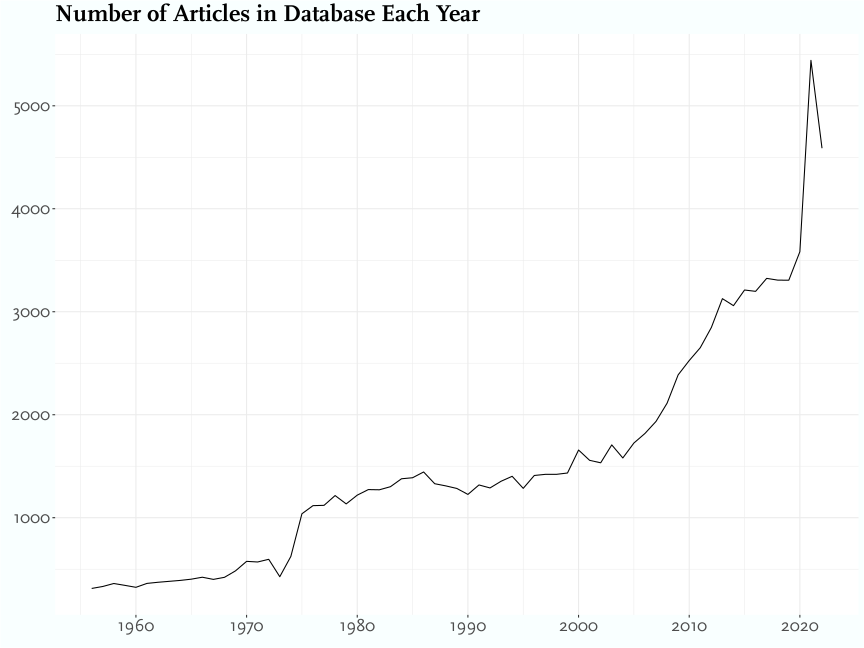
\includegraphics[keepaspectratio]{citations_files/figure-pdf/fig-number-of-articles-by-year-1.pdf}}

}

\caption{\label{fig-number-of-articles-by-year}Number of articles in the
study each year}

\end{figure}%

On top of that, citation practices have changed and people now cite much
more widely than they used to. So the number of citations recorded each
year (to articles since 1956 indexed in these 100 journals), has risen
rather dramatically, as shown in
Figure~\ref{fig-number-of-citations-by-year}.

\begin{figure}

\centering{

\pandocbounded{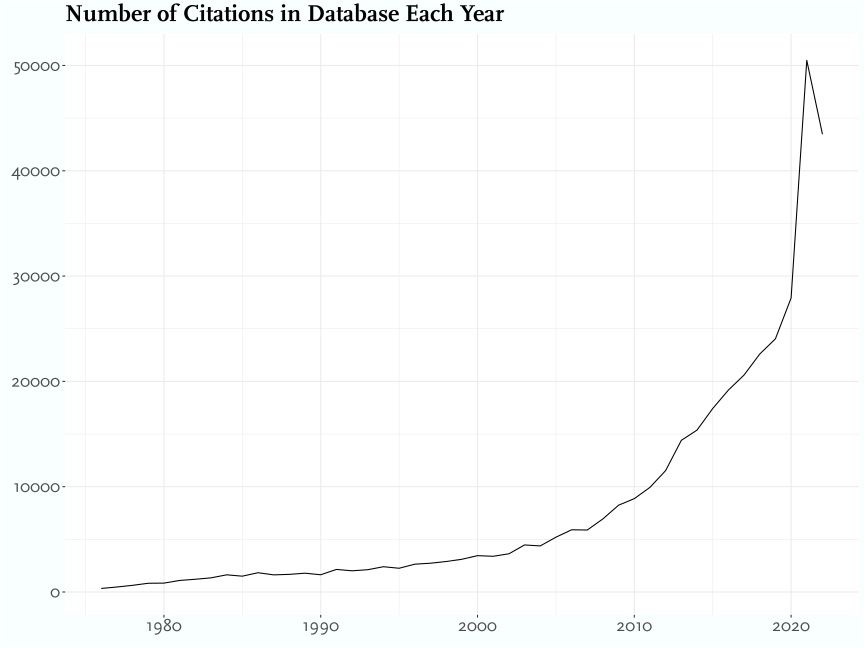
\includegraphics[keepaspectratio]{citations_files/figure-pdf/fig-number-of-citations-by-year-1.pdf}}

}

\caption{\label{fig-number-of-citations-by-year}Number of citations to
articles in the study each year}

\end{figure}%

On the other hand, since the overwhelming majority of citations are to
articles published earlier than the citing article, a larger number of
citations in total might be consistent with fewer citations per article
available to be cited. If we somewhat arbitrarily set the universe of
possible cited papers to be the set of papers with the same publication
date as the citing article or earlier,
Figure~\ref{fig-average-of-citations-by-year} shows how often the
average paper was cited each year (in these 100 journals).

\begin{figure}

\centering{

\pandocbounded{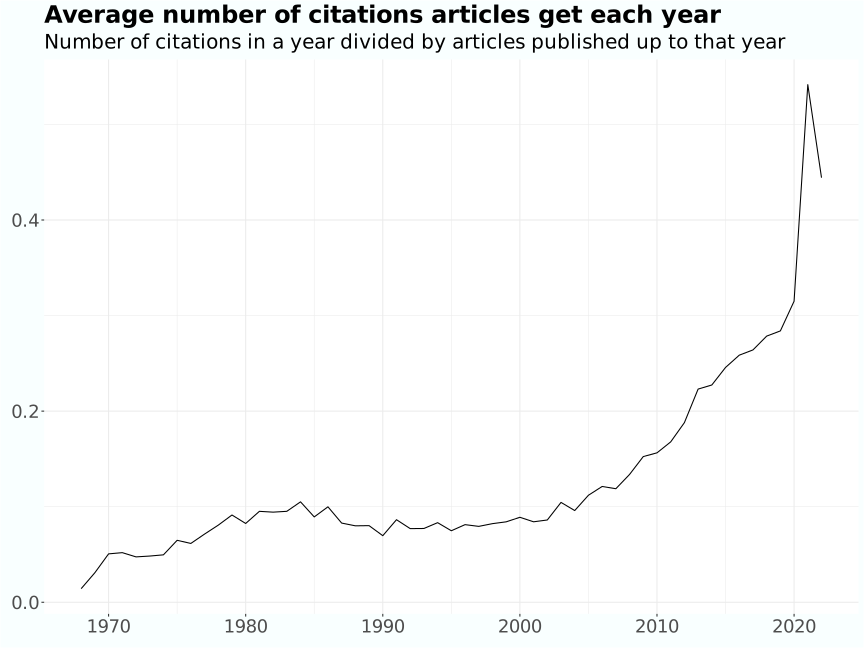
\includegraphics[keepaspectratio]{citations_files/figure-pdf/fig-average-of-citations-by-year-1.pdf}}

}

\caption{\label{fig-average-of-citations-by-year}Average number of
citations per available article in each each year}

\end{figure}%

Between about 1978 and 2004, the different forces are roughly balanced.
There are more papers, and each paper cites more often, but there are
more papers available to be cited, and the mean stays at about 0.1. (Of
course articles do get cited outside of journals indexed in Web of
Science, but it's still a bit humbling to realise that's the historical
average, even if one gets published in a journal as good as one of
these.) But then the forces pushing this number up take over. This is
important context for a lot of the graphs below, where the typical
article will have a graph of citations per year that looks a bit like
this.

\subsection{The Focus}\label{sec-focus}

For each year up to 2020, I made three lists. (After 2020 the citation
data is all too new to be particularly useful I think.) First, a list of
the articles published that year sorted by how many times they are
cited. Second, the same list sorted by how many times they are cited in
what I call \emph{early} years. That's either the first ten years after
publication, or half of the time between publication and 2022, whichever
is shorter. Third, the same list sorted by how many times they are cited
in what I call \emph{late} years, which is either the last ten years of
the study, or the years since publication that are not `early', again
whichever is shorter. Given how many of the citations come from the last
few years, the first and third lists overlap a lot. As we get closer to
the end of the study, the early cites tend to be very volatile, and
there is a bit of impact from how easy journals made it for their papers
to be cited prior to official publication through online early access.

After making those three lists, I found the largest \emph{n} such that
taking the top \emph{n} from those three lists gave me nine total
articles per year. (If forced to choose, I chose the articles with the
most total citations.) So we got a mix largely of highly cited articles,
and articles that were highly cited soon after publication. With nine
articles each year, and sixty-five years between 1956 and 2020, we
should end up with 585 articles.

Having built that list, I decided that articles with fewer than
thirty-four citations (in these 100 journals) were not cited often
enough that it made much sense to talk about trends in their citation
pattern. So I filtered the list down to only include articles with
thirty-four or more citations. The result is that we have 502 articles
in total.

The 502 articles are, for better and for worse, a pretty representative
sample of what was happening in those journals, and in particular what
was being widely talked about in those journals. They wouldn't match up
with my list of the best 502 articles from those forty years, or I
suspect anyone else's list of the best 502 articles. But I do think they
are an interesting model of the field as it was across those years.

It was not a surprise that the famously high prestige journals have the
bulk of these articles. But there was more variation within the list
than some may have expected, as we see in
Table~\ref{tbl-journals-in-main-bib}.

\begin{longtable}[]{@{}lr@{}}

\caption{\label{tbl-journals-in-main-bib}Which journals the 502 articles
appeared in.}

\tabularnewline

\toprule\noalign{}
Journal & Articles \\
\midrule\noalign{}
\endhead
\bottomrule\noalign{}
\endlastfoot
Journal Of Philosophy & 96 \\
Philosophical Review & 69 \\
Philosophical Studies & 40 \\
Noûs & 35 \\
Mind & 31 \\
Philosophy Of Science & 27 \\
Philosophy And Phenomenological Research & 25 \\
Ethics & 19 \\
American Philosophical Quarterly & 18 \\
Philosophy \& Public Affairs & 15 \\
Synthese & 13 \\
Journal Of Philosophical Logic & 11 \\
Philosophical Quarterly & 11 \\
Australasian Journal Of Philosophy & 10 \\
British Journal For The Philosophy Of Science & 9 \\
Analysis & 8 \\
Monist & 8 \\
Linguistics And Philosophy & 5 \\
Inquiry & 4 \\
Pacific Philosophical Quarterly & 4 \\
Philosophers Imprint & 4 \\
Journal Of Symbolic Logic & 3 \\
Mind \& Language & 3 \\
Philosophical Psychology & 3 \\
Philosophy & 3 \\
Biology \& Philosophy & 2 \\
Canadian Journal Of Philosophy & 2 \\
Erkenntnis & 2 \\
Hypatia & 2 \\
Metaphilosophy & 2 \\
Philosophical Perspectives & 2 \\
Ratio & 2 \\
Review Of Metaphysics & 2 \\
Studies In History And Philosophy Of Science & 2 \\
Economics And Philosophy & 1 \\
Episteme & 1 \\
Journal Of Consciousness Studies & 1 \\
Journal Of Medical Ethics & 1 \\
Journal Of Political Philosophy & 1 \\
Journal Of The American Philosophical Association & 1 \\
Philosophia & 1 \\
Philosophy Compass & 1 \\
Social Epistemology & 1 \\
Social Philosophy \& Policy & 1 \\

\end{longtable}

Around half the articles (256 out of 502) are in the journals widely
taken to be the big five: Journal of Philosophy, Philosophical Review,
Mind, Noûs, and Philosophy and Phenomenological Research.

Table~\ref{tbl-recent-journals-in-main-bib} shows what happens if we
restrict attention to just the last fifteen years, and look at which
articles from 2006 to 2020 are widely cited in this sense. The
percentage that are in these five journals falls slightly: it is now 52
out of 120. And the order at the top has changed a bit, as
Table~\ref{tbl-recent-journals-in-main-bib} shows.

\begin{longtable}[]{@{}lr@{}}

\caption{\label{tbl-recent-journals-in-main-bib}Which journals the most
recent 120 articles appeared in.}

\tabularnewline

\toprule\noalign{}
Journal & Articles \\
\midrule\noalign{}
\endhead
\bottomrule\noalign{}
\endlastfoot
Noûs & 19 \\
Philosophical Studies & 18 \\
Philosophy And Phenomenological Research & 10 \\
Mind & 8 \\
Philosophical Review & 8 \\
Journal Of Philosophy & 7 \\
Synthese & 6 \\
Inquiry & 4 \\
Philosophers Imprint & 4 \\
Philosophical Quarterly & 4 \\
Ethics & 3 \\
Australasian Journal Of Philosophy & 2 \\
Biology \& Philosophy & 2 \\
British Journal For The Philosophy Of Science & 2 \\
Erkenntnis & 2 \\
Hypatia & 2 \\
Journal Of Philosophical Logic & 2 \\
Pacific Philosophical Quarterly & 2 \\
Philosophical Perspectives & 2 \\
Philosophy Of Science & 2 \\
Episteme & 1 \\
Journal Of Consciousness Studies & 1 \\
Journal Of Medical Ethics & 1 \\
Journal Of Political Philosophy & 1 \\
Journal Of The American Philosophical Association & 1 \\
Metaphilosophy & 1 \\
Mind \& Language & 1 \\
Monist & 1 \\
Philosophical Psychology & 1 \\
Philosophy Compass & 1 \\
Social Epistemology & 1 \\

\end{longtable}

One thing we see from Table~\ref{tbl-journals-in-main-bib} and
Table~\ref{tbl-recent-journals-in-main-bib} is that \emph{Philosophical
Studies} is a very important journal; it publishes more widely cited
articles than some of the traditionally more prestigious journals. Now
partially that is because it publishes more articles full stop. But
other journals (e.g., \emph{Synthese} and \emph{Erkenntnis}) also
publish a lot of articles without appearing near the top of these
tables.

\subsection{Short Observations}\label{short-observations}

In longer work I plan to make a lot of notes about the data that's
presented here. But for now I'll just note a few things about changes in
the citation patterns over the last forty years.

There are a few reasons that articles might be widely cited immediately
after they come out, and then not so widely cited after a few years.

\begin{itemize}
\tightlist
\item
  The article might get turned into a book, and people simply cite the
  book. You can see that happening in the data below with articles by
  Ted Sider, by John MacFarlane, and by Timothy Williamson, for example.
  It's not part of this study, but not that many people cite Lewis's
  1973 paper on counterfactuals, because they mostly cite his 1973 book
  on counterfactuals. But books don't always soak up the citations that
  papers would otherwise have received. People didn't take the
  discussion of natural properties in \emph{Plurality} to mean they
  should stop citing ``New Work''. Jason Stanley and Timothy
  Williamson's paper on knowing how gets more citations after Stanley's
  book on know how comes out. Still, it is one relatively mundane reason
  that a paper doesn't get much attention.
\item
  The article might simply get superseded. This can happen with
  technical papers in particular. If a paper has some useful technical
  developments, but they are incorporated into later and better work,
  perhaps people just stop citing the earlier work.
\item
  If the article is a negative article, it might simply convince people
  not to pay attention to a particular debate. I suspect this happens a
  bit, but it's hard to find clear cases of it. People didn't stop
  citing \emph{Sense and Sensibilia} when they decided sense-data theory
  had been a mistake, and I suspect that's the more usual situation.
\end{itemize}

Sometimes articles stop getting cited because the philosophical fashion
moves on, and they seem like a relic of an earlier age. You really see
this in the data below with articles about \textbf{supervenience}. Now
I'm enough of an old fashioned intensionalist to think that getting
clear on the different kinds of supervenience is in fact a worthwhile
project. But the discipline as a whole doesn't really agree. Nobody is
citing the work, especially the early work, on different concepts of
supervenience.

What would have been even more shocking to me thirty years ago is how
little attention is paid in the journals now to debates about content
externalism. That felt like the most important debate in philosophy for
so long, and now it simply isn't.

From the other direction, what has picked up the attention? There are
two important things to look at here: new topics, and topics that get
more attention now than they used to. The first one is easy: the big new
topics at the end of the data set are \textbf{conceptual engineering}
and \textbf{grounding}. The second is, to my mind, more interesting.

There are two categories of articles that stand out immediately among
the papers that are more widely cited now than when they first came out.

The biggest of these is \textbf{social philosophy}. In this I'm
including Rae Langton's 1993 article on silencing, Sally Haslanger's
2000 \emph{Noûs} article on race and gender, and Kristie Dotson's 2011
article on epistemic violence. But I'm also including things like
Michael Bratman's 1992 and 1993 articles on collective action. It's a
bit of a stretch, but one might also see the various articles on trust
that show up below (by Annette Baier, Richard Holton, and Karen Jones),
as being of the move towards more social philosophy. Philosophy in the
twentieth century was very focussed on individuals; there is much more
attention now to groups and societies.

The other category is papers on \textbf{probability}. Some papers from
the 1990s, such as Richard Foley's 1992 paper that set out the Lockean
theory of belief, and Jim Joyce's 1998 paper setting up the
accuracy-dominance approoach, are much more widely discussed now than
they were immediately after they came out.

One of my aims with this is to use the co-citation relations between
these 360 papers to find more categories, and especially categories that
are linked by more than my gut feeling that they fit together. But
that's a project for a much longer piece.

\subsection{Future Goals}\label{sec-future-goals}

I'm very interested to hear ideas other people have for what might be
done with this data, and surrounding data. Here are some of the ideas I
have for future research.

The biggest project I've started involves cluster-detection. I've
created a table of how many times each pair of these 360 articles was
co-cited with every other one (among the hundred journals I'm studying).
I've tried running that through various cluster-detecting algorithms to
see if there are naturally occurring clusters of articles. The results
are a bit messy right now, but maybe with some tidying they could be
usefully used to see what trends there are in topics, or in classifying
journals by which kinds of articles they publish.

Otherwise I've got the following tentative ideas.

\begin{itemize}
\tightlist
\item
  Graphing the gender balance among authors over time among these 360
  articles.
\item
  Comparing how widely cited David Lewis's 1980s AJP articles are to how
  widely cited all other articles from the AJP in those years were.
\item
  Looking at how ``Epiphenomenal Qualia'' came to be cited so much more
  than ``What Mary Didn't Know''.
\item
  Separating out age, cohort, and period effects among the various
  trends shown here.
\item
  In particular, looking at the 1986-1990 cohort, and seeing whether the
  relatively low citation numbers shown here are because citations to
  that cohort tended to be more spread out (and so just looking at the
  peaks, like I'm doing here, will miss a lot), or because in general
  later philosophers paid less attention to articles from the late 1980s
  than other eras. And if it's the latter, is that something broader
  about the era, or about the relative importance of journals to other
  publications in that time?
\item
  Looking at the transitions from supervenience, to truthmaking, to
  grounding, in metaphysics over the time of the study, with special
  attention to the connection between that story and the debates about
  physicalism.
\item
  Making a bibtex file for these 460 articles.
\item
  Seeing what connections there are between paper length and number of
  citations.
\item
  Looking at how central papers on equality and egalitarianism are to
  political philosophy over the years.
\item
  Looking at the way the literature on trust developed.
\end{itemize}

But there are lots of other stories here to be investigated, and I'd
love to hear what other ideas people have for what could be done with
it.

\section{The Articles}\label{the-articles}

\begin{longtable}[]{@{}
  >{\raggedright\arraybackslash}p{(\linewidth - 0\tabcolsep) * \real{1.0000}}@{}}
\toprule\noalign{}
\begin{minipage}[b]{\linewidth}\raggedright
Articles
\end{minipage} \\
\midrule\noalign{}
\endhead
\bottomrule\noalign{}
\endlastfoot
Willard van Orman Quine (\citeproc{ref-WOSA1956CEQ2500001}{1956})
``Quantifiers and Propositional Attitudes'' \\
Gottlob Frege (\citeproc{ref-WOSA1956CHJ4400001}{1956}) ``The Thought: A
Logical Inquiry'' \\
H. P. Grice and P. F. Strawson (\citeproc{ref-WOSA1956CGZ5700001}{1956})
``In Defense of a Dogma'' \\
John G. Kemeny and Paul Oppenheim
(\citeproc{ref-WOSA1956CFA0700002}{1956}) ``On Reduction'' \\
H. P. Grice (\citeproc{ref-WOSA1957CGZ6000005}{1957}) ``Meaning'' \\
Zeno Vendler (\citeproc{ref-WOSA1957CCQ4200001}{1957}) ``Verbs and
Times'' \\
G. E. M. Anscombe (\citeproc{ref-WOSA1958CDL1000001}{1958}) ``Modern
Moral Philosophy'' \\
John R. Searle (\citeproc{ref-WOSA1958CCP4400002}{1958}) ``Proper
Names'' \\
John Rawls (\citeproc{ref-WOSA1958CGZ6200002}{1958}) ``Justice as
Fairness'' \\
Stuart Hampshire and H. L. A. Hart
(\citeproc{ref-WOSA1958CGZ9600001}{1958}) ``Decision, Intention and
Certainty'' \\
J. J. C. Smart (\citeproc{ref-WOSA1959CGZ6600001}{1959}) ``Sensations
and Brain Processes'' \\
Frank Sibley (\citeproc{ref-WOSA1959CGZ6800001}{1959}) ``Aesthetic
Concepts'' \\
A. N. Prior (\citeproc{ref-WOSA1959CDK2600002}{1959}) ``Thank Goodness
That''s Over'' \\
Karl R. Popper (\citeproc{ref-WOSA1959CGZ2000003}{1959}) ``The
Propensity Interpretation of Probability'' \\
Michael Dummett (\citeproc{ref-WOSA1959CGZ6700003}{1959})
``Wittgenstein's Philosophy of Mathematics'' \\
Peter T. Geach (\citeproc{ref-WOSA1960CCQ4500006}{1960})
``Ascriptivism'' \\
Norman Malcolm (\citeproc{ref-WOSA1960CCQ4400003}{1960}) ``Anselm's
Ontological Arguments'' \\
J. J. C. Smart (\citeproc{ref-WOSA1961CCP4900001}{1961}) ``Free-Will,
Praise and Blame'' \\
J. R. Lucas (\citeproc{ref-WOSA1961CDK3300002}{1961}) ``Minds, Machines
and Gödel'' \\
I. J. Good (\citeproc{ref-WOSA1961CFT2300005}{1961}) ``A Causal Calculus
(I)'' \\
Hilary Putnam (\citeproc{ref-WOSA1962CET8000004}{1962}) ``It Ain't
Necessarily So'' \\
E. J. Lemmon (\citeproc{ref-WOSA1962CGX0600001}{1962}) ``Moral
Dilemmas'' \\
John R. Searle (\citeproc{ref-WOSA1962CGX0800001}{1962}) ``Meaning and
Speech Acts'' \\
Jaako Hintikka (\citeproc{ref-WOSA1962CGX0500001}{1962}) ``Cogito, Ergo
Sum: Inference or Performance?'' \\
Arthur Danto (\citeproc{ref-WOSA1964CEU2900005}{1964}) ``The
Artworld'' \\
P. F. Strawson (\citeproc{ref-WOSA1964CGZ7200001}{1964}) ``Intention and
Convention in Speech Acts'' \\
John R. Searle (\citeproc{ref-WOSA1964CGZ6900003}{1964}) ``How To Derive
Ought From Is'' \\
Michael Dummett (\citeproc{ref-WOSA1964CGZ7100003}{1964}) ``Bringing
About the Past'' \\
George Dickie (\citeproc{ref-WOSA1964CKG3400005}{1964}) ``The Myth of
the Aesthetic Attitude'' \\
Paul Benacerraf (\citeproc{ref-WOSA1965CGZ7300005}{1965}) ``What Numbers
Could Not Be'' \\
Gilbert Harman (\citeproc{ref-WOSA1965CGZ7300007}{1965}) ``The Inference
To the Best Explanation'' \\
Peter T. Geach (\citeproc{ref-WOSA1965CGZ7600002}{1965})
``Assertion'' \\
J. L. Mackie (\citeproc{ref-WOSA1965CKS0700001}{1965}) ``Causes and
Conditions'' \\
Richard Rorty (\citeproc{ref-WOSA1965CJV5800002}{1965}) ``Mind-Body
Identity, Privacy, and Categories'' \\
David L. Hull (\citeproc{ref-WOSA1965CFT3500004}{1965}) ``The Effect of
Essentialism on Taxonomy: 2000 Years of Stasis (I)'' \\
Frank Sibley (\citeproc{ref-WOSA1965CGZ7400001}{1965}) ``Aesthetic and
Non-Aesthetic'' \\
Joel Feinberg (\citeproc{ref-WOSA1965CJR9200004}{1965}) ``The Expressive
Function of Punishment'' \\
Keith S. Donnellan (\citeproc{ref-WOSA1966ZC83800001}{1966}) ``Reference
and Definite Descriptions'' \\
David Lewis (\citeproc{ref-WOSA1966ZC30400002}{1966}) ``An Argument for
the Identity Theory'' \\
C. B. Martin and Max Deutscher (\citeproc{ref-WOSA1966ZC83700002}{1966})
``Remembering'' \\
Bas C. van Fraassen (\citeproc{ref-WOSA1966ZC32000001}{1966}) ``Singular
Terms, Truth-Value Gaps, and Free Logic'' \\
Jaegwon Kim (\citeproc{ref-WOSA1966ZJ00300003}{1966}) ``On the
Psycho-Physical Identity Theory'' \\
Roderick M. Chisholm and Ernest Sosa
(\citeproc{ref-WOSA1966ZJ00300005}{1966}) ``Logic of Intrinsically
Better'' \\
Donald Davidson (\citeproc{ref-WOSA1967ZP14500007}{1967b}) ``Truth and
Meaning'' \\
Alvin I. Goldman (\citeproc{ref-WOSA1967ZC33900001}{1967}) ``A Causal
Theory of Knowing'' \\
Donald Davidson (\citeproc{ref-WOSA1967ZC34800001}{1967a}) ``Causal
Relations'' \\
Hector-Neri Castañeda (\citeproc{ref-WOSA1967ZH25100001}{1967})
``Indicators and Quasi-Indicators'' \\
Kenneth F. Schaffner (\citeproc{ref-WOSA1967ZC89200003}{1967})
``Approaches To Reduction'' \\
Hilary Putnam (\citeproc{ref-WOSA1967ZC33500002}{1967}) ``Time and
Physical Geometry'' \\
Ian Hacking (\citeproc{ref-WOSA1967ZC89400002}{1967b}) ``Slightly More
Realistic Personal Probability'' \\
Ian Hacking (\citeproc{ref-WOSA1967ZC84100001}{1967a})
``Possibility'' \\
David Lewis (\citeproc{ref-WOSA1968ZE29500001}{1968}) ``Counterpart
Theory and Quantified Modal Logic'' \\
Sydney Shoemaker (\citeproc{ref-WOSA1968ZE30900001}{1968})
``Self-Reference and Self-Awareness'' \\
Barry Stroud (\citeproc{ref-WOSA1968ZE29900001}{1968}) ``Transcendental
Arguments'' \\
Peter Unger (\citeproc{ref-WOSA1968ZE29600001}{1968}) ``An Analysis of
Factual Knowledge'' \\
Herbert Morris (\citeproc{ref-WOSA1968ZL99200001}{1968}) ``Persons and
Punishment'' \\
Willard van Orman Quine (\citeproc{ref-WOSA1968ZE29700001}{1968})
``Ontological Relativity'' \\
Bas C. van Fraassen (\citeproc{ref-WOSA1968ZE29500003}{1968})
``Presupposition, Implication, and Self-Reference'' \\
Gilbert Harman (\citeproc{ref-WOSA1968ZB45300003}{1968}) ``Knowledge,
Inference, and Explanation'' \\
Harry G. Frankfurt (\citeproc{ref-WOSA1969Y444700002}{1969}) ``Alternate
Possibilities and Moral Responsibility'' \\
H. P. Grice (\citeproc{ref-WOSA1969Y406100001}{1969}) ``Utterer's
Meaning and Intentions'' \\
Keith Lehrer and Thomas Paxson Jr.
(\citeproc{ref-WOSA1969Y443200001}{1969}) ``Knowledge: Undefeated
Justified True Belief'' \\
Bas C. van Fraassen (\citeproc{ref-WOSA1969Y443900001}{1969}) ``Facts
and Tautological Entailments'' \\
J. A. Goguen (\citeproc{ref-WOSA1969ZP70500001}{1969}) ``The Logic of
Inexact Concepts'' \\
Fred Dretske (\citeproc{ref-WOSA1970ZE33800001}{1970}) ``Epistemic
Operators'' \\
David Lewis (\citeproc{ref-WOSA1970ZE32700001}{1970}) ``How To Define
Theoretical Terms'' \\
Kendall L. Walton (\citeproc{ref-WOSA1970Y384700002}{1970}) ``Categories
of Art'' \\
Robert Stalnaker (\citeproc{ref-WOSA1970G279500005}{1970}) ``Probability
and Conditionals'' \\
Sydney Shoemaker (\citeproc{ref-WOSA1970Y183500001}{1970}) ``Persons and
Their Pasts'' \\
Willard van Orman Quine (\citeproc{ref-WOSA1970ZE32000003}{1970}) ``On
the Reasons for Indeterminacy of Translation'' \\
Bas C. van Fraassen (\citeproc{ref-WOSA1970H499300001}{1970}) ``On
Extension of Beths Semantics of Physical Theories'' \\
Richard Rorty (\citeproc{ref-WOSA1970ZE32600001}{1970})
``Incorrigibility as Mark of Mental'' \\
Harry G. Frankfurt (\citeproc{ref-10.2307_2024717}{1971}) ``Freedom of
the Will and the Concept of a Person'' \\
Judith Jarvis Thomson (\citeproc{ref-WOSA1971Y116900003}{1971}) ``A
Defense of Abortion'' \\
Derek Parfit (\citeproc{ref-WOSA1971Y036400001}{1971}) ``Personal
Identity'' \\
D. C. Dennett (\citeproc{ref-10.2307_2025382}{1971}) ``Intentional
Systems'' \\
David Lewis (\citeproc{ref-10.2307_2024902}{1971}) ``Counterparts of
Persons and Their Bodies'' \\
George Boolos (\citeproc{ref-10.2307_2025204}{1971}) ``The Iterative
Conception of Set'' \\
William P. Alston (\citeproc{ref-WOSA1971Y185900002}{1971}) ``Varieties
of Privileged Access'' \\
R. Eugene Bales (\citeproc{ref-WOSA1971Y185900004}{1971})
``Act-Utilitarianism: Account of Right-Making Characteristics or
Decision-Making Procedure'' \\
Alvin I. Goldman (\citeproc{ref-10.2307_2024949}{1971}) ``The
Individuation of Action'' \\
Peter Singer (\citeproc{ref-WOSA1972Z066400001}{1972}) ``Famine,
Affluence, and Morality'' \\
Hartry Field (\citeproc{ref-10.2307_2024879}{1972}) ``Tarski's Theory of
Truth'' \\
Philippa Foot (\citeproc{ref-WOSA1972N845400002}{1972}) ``Morality as a
System of Hypothetical Imperatives'' \\
Ned Block and Jerry A. Fodor (\citeproc{ref-WOSA1972YY85800002}{1972})
``What Psychological States Are Not'' \\
Fred Dretske (\citeproc{ref-WOSA1972N864600001}{1972}) ``Contrastive
Statements'' \\
Richard Rorty (\citeproc{ref-10.2307_2025059}{1972}) ``The World Well
Lost'' \\
Gerald Dworkin (\citeproc{ref-WOSA1972N175300004}{1972})
``Paternalism'' \\
Richard Routley and Robert K. Meyer
(\citeproc{ref-WOSA1972Z110200006}{1972}) ``The Semantics of Entailment
--- II'' \\
David Lewis (\citeproc{ref-10.2307_2025310}{1973}) ``Causation'' \\
Paul Benacerraf (\citeproc{ref-10.2307_2025075}{1973}) ``Mathematical
Truth'' \\
Larry Wright (\citeproc{ref-WOSA1973P242100001}{1973}) ``Functions'' \\
Hilary Putnam (\citeproc{ref-10.2307_2025079}{1973}) ``Meaning and
Reference'' \\
Hartry Field (\citeproc{ref-10.2307_2025110}{1973}) ``Theory Change and
the Indeterminacy of Reference'' \\
Jaegwon Kim (\citeproc{ref-10.2307_2025096}{1973}) ``Causation, Nomic
Subsumption, and the Concept of Event'' \\
Tyler Burge (\citeproc{ref-10.2307_2025107}{1973}) ``Reference and
Proper Names'' \\
Michael Walzer (\citeproc{ref-WOSA1973R219800003}{1973}) ``Political
Action: The Problem of Dirty Hands'' \\
Elie Zahar (\citeproc{ref-WOSA1973Q107900001}{1973}) ``Why Did Einsteins
Programme Supersede Lorentzs (I)'' \\
Thomas Nagel (\citeproc{ref-WOSA1974U469700001}{1974}) ``What is It Like
To Be a Bat'' \\
Michael Friedman (\citeproc{ref-10.2307_2024924}{1974}) ``Explanation
and Scientific Understanding'' \\
Isaac Levi (\citeproc{ref-10.2307_2025161}{1974}) ``On Indeterminate
Probabilities'' \\
Keith S. Donnellan (\citeproc{ref-WOSA1974R925600001}{1974}) ``Speaking
of Nothing'' \\
Charles Parsons (\citeproc{ref-WOSA1974U793100003}{1974}) ``The Liar
Paradox'' \\
Peter Singer (\citeproc{ref-WOSA1974U371600008}{1974}) ``Sidgwick and
Reflective Equilibrium'' \\
Michael Devitt (\citeproc{ref-10.2307_2025347}{1974}) ``Singular
Terms'' \\
Saul Kripke (\citeproc{ref-WOSA1975BF60000005}{1975}) ``Outline of a
Theory of Truth'' \\
Robert Cummins (\citeproc{ref-WOSA1975BF60100001}{1975}) ``Functional
Analysis'' \\
Gary Watson (\citeproc{ref-WOSA1975W282300001}{1975}) ``Free Agency'' \\
Allan Gibbard (\citeproc{ref-WOSA1975AU08300005}{1975}) ``Contingent
Identity'' \\
Robert C. Stalnaker (\citeproc{ref-WOSA1975LD17700007}{1975})
``Indicative Conditionals'' \\
Gilbert Harman (\citeproc{ref-WOSA1975V416000001}{1975}) ``Moral
Relativism Defended'' \\
Dorothy L. Grover, Joseph L. Camp Jr., and Nuel D. Belnap Jr.
(\citeproc{ref-WOSA1975BC66900001}{1975}) ``A Pro-Sentential Theory of
Truth'' \\
Geoffrey Paul Hellman and Frank Wilson Thompson
(\citeproc{ref-WOSA1975AT43400003}{1975}) ``Physicalism: Ontology,
Determination, and Reduction'' \\
David Kaplan (\citeproc{ref-WOSA1975BF60000006}{1975}) ``Sets, Concepts
and Extensions: How To Russell a Frege-Church'' \\
Alvin I. Goldman (\citeproc{ref-WOSA1976CP00100001}{1976})
``Discrimination and Perceptual Knowledge'' \\
David Lewis (\citeproc{ref-WOSA1976BZ95100001}{1976b}) ``Probabilities
of Conditionals and Conditional Probabilities'' \\
David Lewis (\citeproc{ref-WOSA1976BF01500006}{1976a}) ``Paradoxes of
Time Travel'' \\
Michael Stocker (\citeproc{ref-WOSA1976CB49000002}{1976}) ``The
Schizophrenia of Modern Ethical Theories'' \\
Gilbert Harman (\citeproc{ref-WOSA1976BK58800002}{1976}) ``Practical
Reasoning'' \\
Robert C. Stalnaker (\citeproc{ref-WOSA1976GM48400006}{1976}) ``Possible
Worlds'' \\
J. Michael Dunn (\citeproc{ref-WOSA1976EK38200001}{1976}) ``Intuitive
Semantics for First-Degree Entailments and Coupled Trees'' \\
Robert Merrihew Adams (\citeproc{ref-WOSA1976CB49000003}{1976}) ``Motive
Utilitarianism'' \\
Brian Loar (\citeproc{ref-WOSA1976EK39100001}{1976}) ``The Semantics of
Singular Terms'' \\
John Perry (\citeproc{ref-WOSA1977EA01800002}{1977}) ``Frege on
Demonstratives'' \\
Stephen L. Darwall (\citeproc{ref-WOSA1977EA35800003}{1977}) ``Two Kinds
of Respect'' \\
Fred Dretske (\citeproc{ref-WOSA1977DN52600007}{1977}) ``Laws of
Nature'' \\
Michael Tooley (\citeproc{ref-WOSA1977EQ83600001}{1977}) ``Nature of
Laws'' \\
John M. Taurek (\citeproc{ref-WOSA1977DX39800001}{1977}) ``Should the
Numbers Count?'' \\
Tyler Burge (\citeproc{ref-WOSA1977DH28800002}{1977}) ``Belief De
Re'' \\
Christopher Boorse (\citeproc{ref-WOSA1977ES93500003}{1977}) ``Health as
a Theoretical Concept'' \\
Hartry Field (\citeproc{ref-WOSA1977DN99500001}{1977}) ``Logic, Meaning,
and Conceptual Role'' \\
Hector-Neri Castañeda (\citeproc{ref-WOSA1977DV15800002}{1977})
``Perception, Belief, and Structure of Physical Objects and
Consciousness'' \\
David Lewis (\citeproc{ref-WOSA1978ER30500004}{1978}) ``Truth in
Fiction'' \\
David L. Hull (\citeproc{ref-WOSA1978FR68900001}{1978}) ``A Matter of
Individuality'' \\
Kendall L. Walton (\citeproc{ref-WOSA1978EK23200001}{1978}) ``Fearing
Fictions'' \\
Stephen P. Stich (\citeproc{ref-WOSA1978GH93900001}{1978}) ``Beliefs and
Subdoxastic States'' \\
Harry G. Frankfurt (\citeproc{ref-WOSA1978EL93700010}{1978}) ``The
Problem of Action'' \\
Paul R. Thagard (\citeproc{ref-WOSA1978EP78600002}{1978}) ``The Best
Explanation: Criteria for Theory Choice'' \\
Jaegwon Kim (\citeproc{ref-WOSA1978EL93700009}{1978}) ``Supervenience
and Nomological Incommensurables'' \\
L BonJour (\citeproc{ref-WOSA1978ER30500001}{1978}) ``Can Empirical
Knowledge Have a Foundation?'' \\
Gregory S. Kavka (\citeproc{ref-WOSA1978FB55500001}{1978}) ``Some
Paradoxes of Deterrence'' \\
John Perry (\citeproc{ref-WOSA1979HE39600001}{1979}) ``The Problem of
the Essential Indexical'' \\
David Lewis (\citeproc{ref-WOSA1979JC64200001}{1979a}) ``Attitudes De
Dicto and De Se'' \\
David Lewis (\citeproc{ref-WOSA1979HJ57600007}{1979c}) ``Scorekeeping in
a Language Game'' \\
David Lewis (\citeproc{ref-WOSA1979JB14500003}{1979b}) ``Counterfactual
Dependence and Time's Arrow'' \\
John McDowell (\citeproc{ref-WOSA1979JT33600005}{1979}) ``Virtue and
Reason'' \\
Graham Priest (\citeproc{ref-WOSA1979GW33200004}{1979}) ``The Logic of
Paradox'' \\
Norman Daniels (\citeproc{ref-WOSA1979GW47300003}{1979}) ``Wide
Reflective Equilibrium and Theory Acceptance in Ethics'' \\
Nancy Cartwright (\citeproc{ref-WOSA1979JB14500001}{1979}) ``Causal Laws
and Effective Strategies'' \\
Daniel Lascar and Bruno Poizat (\citeproc{ref-WOSA1979HL22300006}{1979})
``Introduction To Forking'' \\
John Rawls (\citeproc{ref-WOSA1980KH88100001}{1980}) ``Kantian
Constructivism in Moral Theory'' \\
Martin Davies and Lloyd Humberstone
(\citeproc{ref-WOSA1980KA40400001}{1980}) ``Two Notions of
Necessity'' \\
Hilary Putnam (\citeproc{ref-WOSA1980KJ75900004}{1980}) ``Models and
Reality'' \\
Jerrold Levinson (\citeproc{ref-WOSA1980JC98000001}{1980}) ``What a
Musical Work Is'' \\
Elliot Sober (\citeproc{ref-WOSA1980LE33500002}{1980}) ``Evolution,
Population Thinking, and Essentialism'' \\
Ruth Barcan Marcus (\citeproc{ref-WOSA1980JJ63300001}{1980}) ``Moral
Dilemmas and Consistency'' \\
David Lewis (\citeproc{ref-WOSA1980KX78600003}{1980}) ``Veridical
Hallucination and Prosthetic Vision'' \\
Norman Daniels (\citeproc{ref-WOSA1980JZ97600005}{1980}) ``Reflective
Equilibrium and Archimedean Points'' \\
Paul M. Churchland (\citeproc{ref-WOSA1981LD54600001}{1981})
``Eliminative Materialism and the Propositional Attitudes'' \\
Larry Laudan (\citeproc{ref-WOSA1981LY92900002}{1981}) ``A Confutation
of Convergent Realism'' \\
Philip Kitcher (\citeproc{ref-WOSA1981NA08400001}{1981}) ``Explanatory
Unification'' \\
Jon Barwise and Robin Cooper (\citeproc{ref-WOSA1981LH67300001}{1981})
``Generalized Quantifiers and Natural-Language'' \\
Ronald Dworkin (\citeproc{ref-WOSA1981MH21100001}{1981b}) ``What is
Equality? Part 2: Equality of Resources'' \\
David Lewis (\citeproc{ref-WOSA1981LW58400001}{1981}) ``Causal Decision
Theory'' \\
Peter van Inwagen (\citeproc{ref-WOSA1981LV91400003}{1981}) ``The
Doctrine of Arbitrary Undetached Parts'' \\
Ronald Dworkin (\citeproc{ref-WOSA1981LU74200001}{1981a}) ``What is
Equality (I) Equality of Welfare'' \\
John Dupré (\citeproc{ref-WOSA1981KZ94600003}{1981}) ``Natural Kinds and
Biological Taxa'' \\
Frank Jackson (\citeproc{ref-WOSA1982NH65300003}{1982}) ``Epiphenomenal
Qualia'' \\
Susan Wolf (\citeproc{ref-WOSA1982PB73200001}{1982}) ``Moral Saints'' \\
Elizabeth W. Prior, Robert Pargetter, and Frank Jackson
(\citeproc{ref-WOSA1982NS00700005}{1982}) ``Three Theses About
Dispositions'' \\
Chris Swoyer (\citeproc{ref-WOSA1982PM91600001}{1982}) ``The Nature of
Natural Laws'' \\
Anil Gupta (\citeproc{ref-WOSA1982NW89300001}{1982}) ``Truth and
Paradox'' \\
David Lewis (\citeproc{ref-WOSA1982PN18900005}{1982}) ``Logic for
Equivocators'' \\
Jaegwon Kim (\citeproc{ref-WOSA1982NC90700004}{1982}) ``Psychophysical
Supervenience'' \\
Harry G. Frankfurt (\citeproc{ref-WOSA1982PX46500008}{1982}) ``The
Importance of What We Care About'' \\
Dudley Shapere (\citeproc{ref-WOSA1982PW68500001}{1982}) ``The Concept
of Observation in Science and Philosophy'' \\
David Lewis (\citeproc{ref-WOSA1983RR51600001}{1983}) ``New Work for a
Theory of Universals'' \\
Joseph Levine (\citeproc{ref-WOSA1983SU49200007}{1983}) ``Materialism
and Qualia: The Explanatory Gap'' \\
Gregory S. Kavka (\citeproc{ref-WOSA1983PX89100011}{1983}) ``The Toxin
Puzzle'' \\
Christine M. Korsgaard (\citeproc{ref-WOSA1983QN98800001}{1983}) ``Two
Distinctions in Goodness'' \\
Robert Brandom (\citeproc{ref-WOSA1983RV45200006}{1983})
``Asserting'' \\
Judith Jarvis Thomson (\citeproc{ref-WOSA1983QK97500001}{1983})
``Parthood and Identity Across Time'' \\
Hilary Kornblith (\citeproc{ref-WOSA1983PZ01000002}{1983}) ``Justified
Belief and Epistemically Responsible Action'' \\
Alvin Plantinga (\citeproc{ref-WOSA1983QU18900001}{1983}) ``On
Existentialism'' \\
Ellery Eells and Elliot Sober (\citeproc{ref-WOSA1983QJ85300002}{1983})
``Probabilistic Causality and the Question of Transitivity'' \\
David Lewis (\citeproc{ref-WOSA1984TQ70900001}{1984}) ``Putnam's
Paradox'' \\
Bas C. van Fraassen (\citeproc{ref-WOSA1984SS95000001}{1984}) ``Belief
and the Will'' \\
Peter Railton (\citeproc{ref-WOSA1984SH40600002}{1984}) ``Alienation,
Consequentialism, and the Demands of Morality'' \\
George Boolos (\citeproc{ref-WOSA1984TE24500002}{1984}) ``To Be is To Be
a Value of a Variable (Or To Be Some Values of Some Variables)'' \\
Jaegwon Kim (\citeproc{ref-WOSA1984TV24600001}{1984}) ``Concepts of
Supervenience'' \\
Stewart Cohen (\citeproc{ref-WOSA1984TN86300001}{1984}) ``Justification
and Truth'' \\
Philip Kitcher (\citeproc{ref-WOSA1984SZ73700006}{1984}) ``Species'' \\
Kevin Mulligan, Peter Simons, and Barry Smith
(\citeproc{ref-WOSA1984SE25700001}{1984}) ``Truth-Makers'' \\
Jerry Fodor (\citeproc{ref-WOSA1984SL56000004}{1984}) ``Observation
Reconsidered'' \\
Carlos E. Alchourrón, Peter Gärdenfors, and David Makinson
(\citeproc{ref-WOSA1985AKA2200025}{1985}) ``On the Logic of Theory
Change: Partial Meet Contraction and Revision Functions'' \\
Richard Feldman and Earl Conee (\citeproc{ref-WOSA1985ANT6600002}{1985})
``Evidentialism'' \\
John Hardwig (\citeproc{ref-WOSA1985ALK4200001}{1985}) ``Epistemic
Dependence'' \\
Ernan McMullin (\citeproc{ref-WOSA1985ARQ5600003}{1985}) ``Galilean
Idealization'' \\
Vann McGee (\citeproc{ref-WOSA1985AQZ7400002}{1985}) ``A Counterexample
To Modus Ponens'' \\
John Rawls (\citeproc{ref-WOSA1985APA8500001}{1985}) ``Justice as
Fairness: Political Not Metaphysical'' \\
William P. Alston (\citeproc{ref-WOSA1985AML6300004}{1985}) ``Concepts
of Epistemic Justification'' \\
Richard Feldman (\citeproc{ref-WOSA1985APJ3700001}{1985}) ``Reliability
and Justification'' \\
Paul M. Churchland (\citeproc{ref-WOSA1985AAC6100002}{1985})
``Reduction, Qualia, and the Direct Introspection of Brain States'' \\
Peter Railton (\citeproc{ref-WOSA1986C044900001}{1986}) ``Moral
Realism'' \\
Tyler Burge (\citeproc{ref-WOSA1986AYX3200001}{1986a}) ``Individualism
and Psychology'' \\
Annette Baier (\citeproc{ref-WOSA1986AYY3900001}{1986}) ``Trust and
Antitrust'' \\
Christine M. Korsgaard (\citeproc{ref-WOSA1986AYQ1300001}{1986})
``Skepticism About Practical Reason'' \\
David M. Rosenthal (\citeproc{ref-WOSA1986C316000003}{1986}) ``Two
Concepts of Consciousness'' \\
Frank Jackson and Robert Pargetter
(\citeproc{ref-WOSA1986C044900003}{1986}) ``Oughts, Options, and
Actualism'' \\
Tyler Burge (\citeproc{ref-WOSA1986F231300001}{1986b}) ``Intellectual
Norms and Foundations of Mind'' \\
Ruth Garrett Millikan (\citeproc{ref-WOSA1986AYX3200002}{1986})
``Thoughts Without Laws, Cognitive Science With Content'' \\
M Smith (\citeproc{ref-WOSA1987F993300003}{1987}) ``The Humean Theory of
Motivation'' \\
Harry G. Frankfurt (\citeproc{ref-WOSA1987M543000002}{1987}) ``Equality
as a Moral Ideal'' \\
John Bigelow and Robert Pargetter
(\citeproc{ref-WOSA1987G947600001}{1987}) ``Functions'' \\
John Earman and John Norton (\citeproc{ref-WOSA1987M488500005}{1987})
``What Price Spacetime Substantivalism: The Hole Story'' \\
DW Stampe (\citeproc{ref-WOSA1987J665800001}{1987}) ``The Authority of
Desire'' \\
LS Temkin (\citeproc{ref-WOSA1987H340500002}{1987}) ``Intransitivity and
the Mere Addition Paradox'' \\
Thomas Nagel (\citeproc{ref-WOSA1987J379200001}{1987}) ``Moral Conflict
and Political Legitimacy'' \\
M Gilbert (\citeproc{ref-WOSA1987K730800008}{1987}) ``Modeling
Collective Belief'' \\
Larry Laudan (\citeproc{ref-WOSA1987F902200002}{1987}) ``Progress or
Rationality: The Prospects for Normative Naturalism'' \\
Tyler Burge (\citeproc{ref-WOSA1988R020000007}{1988}) ``Individualism
and Self-Knowledge'' \\
James Bogen and James Woodward (\citeproc{ref-WOSA1988N938600001}{1988})
``Saving the Phenomena'' \\
A Grove (\citeproc{ref-WOSA1988M958800004}{1988}) ``Two Modelings for
Theory Change'' \\
K Sterelny and Philip Kitcher (\citeproc{ref-WOSA1988P217100001}{1988})
``The Return of the Gene'' \\
S Kagan (\citeproc{ref-WOSA1988Q913800001}{1988}) ``The Additive
Fallacy'' \\
William P. Alston (\citeproc{ref-WOSA1988M863300002}{1988}) ``An
Internalist Externalism'' \\
David Lewis (\citeproc{ref-WOSA1988P549200001}{1988}) ``Desire as
Belief'' \\
Frank Jackson and Philip Pettit
(\citeproc{ref-WOSA1988P549200004}{1988}) ``Functionalism and Broad
Content'' \\
John Rawls (\citeproc{ref-WOSA1988Q394000001}{1988}) ``The Priority of
Right and Ideas of the Good'' \\
G. A. Cohen (\citeproc{ref-WOSA1989AE70300010}{1989}) ``On the Currency
of Egalitarian Justice'' \\
Ruth Garrett Millikan (\citeproc{ref-WOSA1989AA09400006}{1989b}) ``In
Defense of Proper Functions'' \\
Ruth Garrett Millikan (\citeproc{ref-WOSA1989U850300001}{1989a})
``Biosemantics'' \\
Paul A. Boghossian and J. David Velleman
(\citeproc{ref-WOSA1989T231400005}{1989}) ``Color as a Secondary
Quality'' \\
RJ Arneson (\citeproc{ref-WOSA1989U808000004}{1989}) ``Equality and
Equal Opportunity for Welfare'' \\
Paul A. Boghossian (\citeproc{ref-WOSA1989CA94000002}{1989}) ``The
Rule-Following Considerations'' \\
M Crimmins and John Perry (\citeproc{ref-WOSA1989CF70700001}{1989})
``The Prince and the Phone Booth: Reporting Puzzling Beliefs'' \\
D Marquis (\citeproc{ref-WOSA1989U039600002}{1989}) ``Why Abortion is
Immoral'' \\
WS Quinn (\citeproc{ref-WOSA1989AV72300002}{1989}) ``Actions,
Intentions, and Consequences: The Doctrine of Double Effect'' \\
Philip Kitcher (\citeproc{ref-WOSA1990CH71200001}{1990}) ``The Division
of Cognitive Labor'' \\
Frank Jackson and Philip Pettit
(\citeproc{ref-WOSA1990CR32400008}{1990}) ``Program Explanation: A
General Perspective'' \\
Donald Davidson (\citeproc{ref-WOSA1990EQ84600001}{1990}) ``The
Structure and Content of Truth'' \\
Gideon Rosen (\citeproc{ref-WOSA1990DR99100001}{1990}) ``Modal
Fictionalism'' \\
Tim Crane and D. H. Mellor (\citeproc{ref-WOSA1990DA14600002}{1990})
``There is No Question of Physicalism'' \\
J Dreier (\citeproc{ref-WOSA1990EK23400001}{1990}) ``Internalism and
Speaker Relativism'' \\
J Vogel (\citeproc{ref-WOSA1990EF94500012}{1990}) ``Cartesian Skepticism
and Inference To the Best Explanation'' \\
Jaegwon Kim (\citeproc{ref-WOSA1990FU75100001}{1990}) ``Supervenience as
a Philosophical Concept'' \\
Graeme Forbes (\citeproc{ref-WOSA1990EB39300002}{1990}) ``The
Indispensability of Sinn'' \\
Daniel C. Dennett (\citeproc{ref-WOSA1991EN62900002}{1991}) ``Real
Patterns'' \\
Karen Neander (\citeproc{ref-WOSA1991FQ15000002}{1991}) ``Functions as
Selected Effects: The Conceptual Analyst's Defense'' \\
Richard Boyd (\citeproc{ref-WOSA1991FC38500010}{1991}) ``Realism,
Anti-foundationalism and the Enthusiasm for Natural Kinds'' \\
Frank Jackson (\citeproc{ref-WOSA1991FK52800001}{1991})
``Decision-theoretic Consequentialism and the Nearest and Dearest
Objection'' \\
Judith Jarvis Thomson (\citeproc{ref-WOSA1991GR79400001}{1991})
``Self-Defense'' \\
J Groenendijk and M Stokhof (\citeproc{ref-WOSA1991EV09800002}{1991})
``Dynamic Predicate Logic'' \\
John Hardwig (\citeproc{ref-WOSA1991GR87800001}{1991}) ``The Role of
Trust in Knowledge'' \\
Stephen Schiffer (\citeproc{ref-WOSA1991EW92800001}{1991}) ``Ceteris
Paribus Laws'' \\
Jerry A. Fodor (\citeproc{ref-WOSA1991EN62900001}{1991}) ``A Modal
Argument for Narrow Content'' \\
Stephen Yablo (\citeproc{ref-WOSA1992JA62400001}{1992}) ``Mental
Causation'' \\
Mark Johnston (\citeproc{ref-WOSA1992KC39800002}{1992}) ``How To Speak
of the Colors'' \\
Keith DeRose (\citeproc{ref-WOSA1992KB29500008}{1992}) ``Contextualism
and Knowledge Attributions'' \\
Jaegwon Kim (\citeproc{ref-WOSA1992HF90400001}{1992}) ``Multiple
Realization and the Metaphysics of Reduction'' \\
ME Bratman (\citeproc{ref-WOSA1992JA62400003}{1992}) ``Shared
Cooperative Activity'' \\
Philip Kitcher (\citeproc{ref-WOSA1992HF90300002}{1992}) ``The
Naturalists Return'' \\
R Foley (\citeproc{ref-WOSA1992JR30700002}{1992}) ``The Epistemology of
Belief and the Epistemology of Degrees of Belief'' \\
Stephen Schiffer (\citeproc{ref-WOSA1992JQ78400001}{1992}) ``Belief
Ascription'' \\
Michael B. Burke (\citeproc{ref-WOSA1992HC13100003}{1992}) ``Copper
Statues and Pieces of Copper: A Challenge To the Standard Account'' \\
Tyler Burge (\citeproc{ref-WOSA1993ML38000001}{1993}) ``Content
Preservation'' \\
Stephen Yablo (\citeproc{ref-WOSA1993KQ63200001}{1993a}) ``Is
Conceivability a Guide To Possibility'' \\
Rae Langton (\citeproc{ref-WOSA1993MJ74900002}{1993}) ``Speech Acts and
Unspeakable Acts'' \\
Stephen Yablo (\citeproc{ref-WOSA1993MG45400010}{1993b}) ``Paradox
Without Self-Reference'' \\
ME Bratman (\citeproc{ref-WOSA1993ME08500006}{1993}) ``Shared
Intention'' \\
T Horgan (\citeproc{ref-WOSA1993ME23100001}{1993}) ``From Supervenience
To Superdupervenience: Meeting the Demands of a Material World'' \\
D Braun (\citeproc{ref-WOSA1993NN82400002}{1993}) ``Empty Names'' \\
P. E. Griffiths (\citeproc{ref-WOSA1993MM47700002}{1993}) ``Functional
Analysis and Proper Functions'' \\
F Dretske (\citeproc{ref-WOSA1993LB00700004}{1993}) ``Conscious
Experience'' \\
David Lewis (\citeproc{ref-WOSA1994PM10400005}{1994}) ``Humean
Supervenience Debugged'' \\
C. B. Martin (\citeproc{ref-WOSA1994MT56900001}{1994}) ``Dispositions
and Conditionals'' \\
Malcom Forster and Elliot Sober
(\citeproc{ref-WOSA1994NQ78600001}{1994}) ``How To Tell When Simpler,
More Unified, or Less \emph{Ad Hoc} Theories Will Provide More Accurate
Predictions'' \\
Hartry Field (\citeproc{ref-WOSA1994NY27600001}{1994}) ``Deflationist
Views of Meaning and Content'' \\
P Godfrey-Smith (\citeproc{ref-WOSA1994PG81700003}{1994}) ``A Modern
History Theory of Functions'' \\
R Holton (\citeproc{ref-WOSA1994NA94600005}{1994}) ``Deciding To Trust,
Coming To Believe'' \\
R Audi (\citeproc{ref-WOSA1994PW69700001}{1994}) ``Dispositional Beliefs
and Dispositions To Believe'' \\
G Strawson (\citeproc{ref-WOSA1994PB07700001}{1994}) ``The Impossibility
of Moral Responsibility'' \\
P. E. Griffiths and R. D. Gray (\citeproc{ref-WOSA1994NP54800001}{1994})
``Developmental Systems and Evolutionary Explanation'' \\
Keith DeRose (\citeproc{ref-WOSA1995RC31600001}{1995}) ``Solving the
Skeptical Problem'' \\
Dorothy Edgington (\citeproc{ref-WOSA1995QX94800001}{1995}) ``On
Conditionals'' \\
T van Gelder (\citeproc{ref-WOSA1995RG53900001}{1995}) ``What Might
Cognition Be, If Not Computation'' \\
D Widerker (\citeproc{ref-WOSA1995TB96300003}{1995}) ``Libertarianism
and Frankfurt's Attack on the Principle of Alternative
Possibilities'' \\
Dean W. Zimmerman (\citeproc{ref-WOSA1995RC31600002}{1995}) ``Theories
of Masses and Problems of Constitution'' \\
N Chomsky (\citeproc{ref-WOSA1995QH55500001}{1995}) ``Language and
Nature'' \\
Karen Neander (\citeproc{ref-WOSA1995RP14800001}{1995})
``Misrepresenting and Malfunctioning'' \\
John McDowell (\citeproc{ref-WOSA1995TH53900008}{1995}) ``Knowledge and
the Internal'' \\
Kit Fine (\citeproc{ref-WOSA1995RD61000003}{1995}) ``The Logic of
Essence'' \\
David Lewis (\citeproc{ref-WOSA1996VY21200001}{1996}) ``Elusive
Knowledge'' \\
Timothy Williamson (\citeproc{ref-WOSA1996XR76100003}{1996}) ``Knowing
and Asserting'' \\
F Veltman (\citeproc{ref-WOSA1996UV93000001}{1996}) ``Defaults in Update
Semantics'' \\
Karen Jones (\citeproc{ref-WOSA1996VL52500002}{1996}) ``Trust as An
Affective Attitude'' \\
Ronald Dworkin (\citeproc{ref-WOSA1996UT36600001}{1996}) ``Objectivity
and Truth: You'd Better Believe It'' \\
Paul A. Boghossian (\citeproc{ref-WOSA1996VJ65500005}{1996})
``Analyticity Reconsidered'' \\
Theodore Sider (\citeproc{ref-WOSA1996VE56300003}{1996}) ``All the
World's a Stage'' \\
A Oliver (\citeproc{ref-WOSA1996TT05300001}{1996}) ``The Metaphysics of
Properties'' \\
Donald Davidson (\citeproc{ref-WOSA1996UM62300001}{1996}) ``The Folly of
Trying To Define Truth'' \\
David Lewis (\citeproc{ref-WOSA1997WP33800001}{1997}) ``Finkish
Dispositions'' \\
Derek Parfit (\citeproc{ref-WOS000070778500002}{1997}) ``Equality and
Priority'' \\
LR Baker (\citeproc{ref-WOS000070661300001}{1997}) ``Why Constitution is
Not Identity'' \\
R Audi (\citeproc{ref-WOS000070790100002}{1997}) ``The Place of
Testimony in the Fabric of Knowledge and Justification'' \\
CS Hill (\citeproc{ref-WOSA1997XH01200003}{1997}) ``Imaginability,
Conceivability, Possibility and the Mind-Body Problem'' \\
Tyler Burge (\citeproc{ref-WOSA1997WT06900002}{1997}) ``Interlocution,
Perception, and Memory'' \\
RM Sainsbury (\citeproc{ref-WOS000071087200008}{1997}) ``Easy
Possibilities'' \\
Susan Wolf (\citeproc{ref-WOSA1997WF56900009}{1997}) ``Happiness and
Meaning: Two Aspects of the Good Life'' \\
MJ Zimmerman (\citeproc{ref-WOSA1997WR70900002}{1997}) ``Moral
Responsibility and Ignorance'' \\
Andy Clark and David J. Chalmers
(\citeproc{ref-WOS000073222300002}{1998}) ``The Extended Mind'' \\
James M. Joyce (\citeproc{ref-WOS000077956100002}{1998}) ``A
Nonpragmatic Vindication of Probabilism'' \\
J Ladyman (\citeproc{ref-WOS000076086400005}{1998}) ``What is Structural
Realism?'' \\
Nathan Salmon (\citeproc{ref-WOS000075762200001}{1998})
``Nonexistence'' \\
Alexander Bird (\citeproc{ref-WOS000072823100011}{1998}) ``Dispositions
and Antidotes'' \\
Rae Langton and David Lewis (\citeproc{ref-WOS000073836400005}{1998})
``Defining `Intrinsic'\,'' \\
Earl Conee and Richard Feldman (\citeproc{ref-WOS000072502200001}{1998})
``The Generality Problem for Reliabilism'' \\
Judith Jarvis Thomson (\citeproc{ref-WOS000073884600001}{1998}) ``The
Statue and the Clay'' \\
John McDowell (\citeproc{ref-WOS000075622500001}{1998}) ``Having the
World in View: Sellars, Kant, and Intentionality: Lecture I: Sellars on
Perceptual Experience'' \\
Elizabeth S. Anderson (\citeproc{ref-WOS000078432400003}{1999}) ``What
is the Point of Equality?'' \\
John Broome (\citeproc{ref-WOS000084073700005}{1999}) ``Normative
Requirements'' \\
Ned Block and Robert Stalnaker (\citeproc{ref-WOS000084347100001}{1999})
``Conceptual Analysis, Dualism, and the Explanatory Gap'' \\
Jaegwon Kim (\citeproc{ref-WOS000082592000002}{1999}) ``Making Sense of
Emergence'' \\
W Bechtel and J Mundale (\citeproc{ref-WOS000080550400001}{1999})
``Multiple Realizability Revisited: Linking Cognitive and Neural
States'' \\
J. David Velleman (\citeproc{ref-WOS000078432400004}{1999}) ``Love as a
Moral Emotion'' \\
Brandon Fitelson (\citeproc{ref-WOS000083295800029}{1999}) ``The
Plurality of Bayesian Measures of Confirmation and the Problem of
Measure Sensitivity'' \\
Tomoji Shogenji (\citeproc{ref-WOS000085486100019}{1999}) ``Is Coherence
Truth Conducive?'' \\
J Hyman (\citeproc{ref-WOS000082596900001}{1999}) ``How Knowledge
Works'' \\
Peter Machamer, Lindley Darden, and Carl F. Craver
(\citeproc{ref-WOS000087305900001}{2000}) ``Thinking About
Mechanisms'' \\
James Pryor (\citeproc{ref-WOS000165361800002}{2000}) ``The Skeptic and
the Dogmatist'' \\
Sally Haslanger (\citeproc{ref-WOS000085841900002}{2000}) ``Gender and
Race: (What) Are They? (What) Do We Want Them To Be?'' \\
David Lewis (\citeproc{ref-WOS000089124200002}{2000}) ``Causation as
Influence'' \\
Justin D'Arms and Dan Jacobson (\citeproc{ref-WOS000087998300003}{2000})
``The Moralistic Fallacy: On the `Appropriateness' of Emotions'' \\
Jason Stanley and Zoltán Gendler Szabó
(\citeproc{ref-WOS000088616400001}{2000}) ``On Quantifier Domain
Restriction'' \\
Heather Douglas (\citeproc{ref-WOS000166575500001}{2000}) ``Inductive
Risk and Values in Science'' \\
Jason Stanley (\citeproc{ref-WOS000088534100002}{2000}) ``Context and
Logical Form'' \\
Adam Elga (\citeproc{ref-WOS000086383700001}{2000}) ``Self-Locating
Belief and the `Sleeping Beauty' Problem'' \\
Jason Stanley and Timothy Williamson
(\citeproc{ref-WOS000170277300002}{2001}) ``Knowing How'' \\
Alex Byrne (\citeproc{ref-WOS000171488600002}{2001}) ``Intentionalism
Defended'' \\
David J. Chalmers and Frank Jackson
(\citeproc{ref-WOS000174798400001}{2001}) ``Conceptual Analysis and
Reductive Explanation'' \\
Alvin I. Goldman (\citeproc{ref-WOS000170434600004}{2001}) ``Experts:
Which Ones Should You Trust?'' \\
C Hitchcock (\citeproc{ref-WOS000169156400001}{2001}) ``The
Intransitivity of Causation Revealed in Equations and Graphs'' \\
Patrick Rysiew (\citeproc{ref-WOS000172282100001}{2001}) ``The
Context-Sensitivity of Knowledge Attributions'' \\
F Adams and K Aizawa (\citeproc{ref-WOS000167688000003}{2001}) ``The
Bounds of Cognition'' \\
Christopher Peacocke (\citeproc{ref-WOS000168307800002}{2001}) ``Does
Perception Have a Nonconceptual Content?'' \\
Carl F. Craver (\citeproc{ref-WOS000167722000004}{2001}) ``Role
Functions, Mechanisms, and Hierarchy'' \\
Michael G. F. Martin (\citeproc{ref-WOS000177781700002}{2002}) ``The
Transparency of Experience'' \\
Jeremy Fantl and Matthew McGrath
(\citeproc{ref-WOS000181094500003}{2002}) ``Evidence, Pragmatics, and
Justification'' \\
Robert C. Stalnaker (\citeproc{ref-WOS000179607800011}{2002}) ``Common
Ground (Speaker Presupposition)'' \\
Stuart Glennan (\citeproc{ref-WOS000178763700030}{2002}) ``Rethinking
Mechanistic Explanation'' \\
Stewart Cohen (\citeproc{ref-WOS000178597300004}{2002}) ``Basic
Knowledge and the Problem of Easy Knowledge'' \\
Ruth Chang (\citeproc{ref-WOS000177540500001}{2002}) ``The Possibility
of Parity'' \\
C Wright (\citeproc{ref-WOS000178597300005}{2002}) ``(Anti-)Sceptics
Simple and Subtle: G.E. Moore and John McDowell'' \\
Mohan Matthen and André Ariew (\citeproc{ref-WOS000173660000001}{2002})
``Two Ways of Thinking About Fitness and Natural Selection'' \\
C List and Philip Pettit (\citeproc{ref-WOS000175194800009}{2002})
``Aggregating Sets of Judgments: An Impossibility Result'' \\
Keith DeRose (\citeproc{ref-WOS000184740400001}{2003}) ``Assertion,
Knowledge, and Context'' \\
Nishi Shah (\citeproc{ref-WOS000224335200001}{2003}) ``How Truth Governs
Belief'' \\
Joshua Knobe (\citeproc{ref-WOS000183806600005}{2003}) ``Intentional
Action and Side Effects in Ordinary Language'' \\
A Hájek (\citeproc{ref-WOS000186731300001}{2003}) ``What Conditional
Probability Could Not Be'' \\
Tyler Burge (\citeproc{ref-WOS000188410400001}{2003}) ``Perceptual
Entitlement'' \\
Thomas Kelly (\citeproc{ref-WOS000183034300004}{2003}) ``Epistemic
Rationality as Instrumental Rationality: A Critique'' \\
Jonathan Schaffer (\citeproc{ref-WOS000184542900005}{2003}) ``Is There a
Fundamental Level?'' \\
John MacFarlane (\citeproc{ref-WOS000183846000001}{2003}) ``Future
Contingents and Relative Truth'' \\
Kit Fine (\citeproc{ref-WOS000182357000001}{2003}) ``The Non-Identity of
a Material Thing and Its Matter'' \\
Wlodek Rabinowicz and Toni Rønnow‐Rasmussen
(\citeproc{ref-WOS000222134800001}{2004}) ``The Strike of the Demon: On
Fitting Pro-Attitudes and Value'' \\
Charles Travis (\citeproc{ref-WOS000188660700003}{2004}) ``The Silence
of the Senses'' \\
Michael G. F. Martin (\citeproc{ref-WOS000223334900003}{2004}) ``The
Limits of Self-Awareness'' \\
David Pitt (\citeproc{ref-WOS000223274200001}{2004}) ``The Phenomenology
of Cognition, Or, What is It Like To Think That P?'' \\
RD Rupert (\citeproc{ref-WOS000223963700001}{2004}) ``Challenges To the
Hypothesis of Extended Cognition'' \\
Mark Johnston (\citeproc{ref-WOS000223334900005}{2004}) ``The Obscure
Object of Hallucination'' \\
RN Giere (\citeproc{ref-WOS000228600800009}{2004}) ``How Models Are Used
To Represent Reality'' \\
David J. Chalmers (\citeproc{ref-WOS000220800700007}{2004}) ``Epistemic
Two-Dimensional Semantics'' \\
J Mcmahan (\citeproc{ref-WOS000224317900003}{2004}) ``The Ethics of
Killing in War'' \\
Niko Kolodny (\citeproc{ref-WOS000231037900002}{2005}) ``Why Be
Rational?'' \\
Nishi Shah and J. David Velleman
(\citeproc{ref-WOS000240571800003}{2005}) ``Doxastic Deliberation'' \\
Angela M. Smith (\citeproc{ref-WOS000227058600002}{2005})
``Responsibility for Attitudes: Activity and Passivity in Mental
Life'' \\
P Lasersohn (\citeproc{ref-WOS000236414800001}{2005}) ``Context
Dependence, Disagreement, and Predicates of Personal Taste'' \\
Pamela Hieronymi (\citeproc{ref-WOS000234618400001}{2005}) ``The Wrong
Kind of Reason'' \\
Matthew Weiner (\citeproc{ref-WOS000240474600003}{2005}) ``Must We Know
What We Say?'' \\
Alan Baker (\citeproc{ref-WOS000228926500001}{2005}) ``Are There Genuine
Mathematical Explanations of Physical Phenomena?'' \\
Timothy Williamson (\citeproc{ref-WOS000228214500004}{2005})
``Contextualism, Subject-Sensitive Invariantism and Knowledge of
Knowledge'' \\
E Nahmias, S Morris, T Nadelhoffer, and J Turner
(\citeproc{ref-WOS000232807900002}{2005}) ``Surveying Freedom: Folk
Intuitions About Free Will and Moral Responsibility'' \\
Sharon Street (\citeproc{ref-WOS000234431300006}{2006}) ``A Darwinian
Dilemma for Realist Theories of Value'' \\
Hilary Greaves and David Wallace
(\citeproc{ref-WOS000239761400003}{2006}) ``Justifying
Conditionalization: Conditionalization Maximizes Expected Epistemic
Utility'' \\
Igor Douven (\citeproc{ref-WOS000207419100002}{2006}) ``Assertion,
Knowledge, and Rational Credibility'' \\
Carl F. Craver (\citeproc{ref-WOS000242288200003}{2006}) ``When
Mechanistic Models Explain'' \\
Peter Godfrey-Smith (\citeproc{ref-WOS000244292800007}{2006}) ``The
Strategy of Model-Based Science'' \\
Roger White (\citeproc{ref-WOS000243445600002}{2006}) ``Problems for
Dogmatism'' \\
David Enoch (\citeproc{ref-WOS000207418900002}{2006}) ``Agency,
Shmagency: Why Normativity Won't Come From What is Constitutive of
Action'' \\
Nishi Shah (\citeproc{ref-WOS000240552100001}{2006}) ``A New Argument
for Evidentialism'' \\
Joshua Knobe (\citeproc{ref-WOS000240410600002}{2006}) ``The Concept of
Intentional Action: A Case Study in the Uses of Folk Psychology'' \\
Adam Elga (\citeproc{ref-WOS000249103800005}{2007}) ``Reflection and
Disagreement'' \\
David Christensen (\citeproc{ref-WOS000207419300002}{2007})
``Epistemology of Disagreement: The Good News'' \\
Seth Yalcin (\citeproc{ref-WOS000251545300007}{2007}) ``Epistemic
Modals'' \\
Jennifer Lackey (\citeproc{ref-WOS000250773100002}{2007}) ``Norms of
Assertion'' \\
Michael Huemer (\citeproc{ref-WOS000246866000002}{2007}) ``Compassionate
Phenomenal Conservatism'' \\
Michael Weisberg (\citeproc{ref-WOS000255137700002}{2007}) ``Three Kinds
of Idealization'' \\
Andy Egan (\citeproc{ref-WOS000245280800001}{2007}) ``Epistemic Modals,
Relativism and Assertion'' \\
John MacFarlane (\citeproc{ref-WOS000244463400002}{2007}) ``Relativism
and Disagreement'' \\
Shaun Nichols and Joshua Knobe (\citeproc{ref-WOS000250773100004}{2007})
``Moral Responsibility and Determinism: The Cognitive Science of Folk
Intuitions'' \\
John Hawthorne and Jason Stanley
(\citeproc{ref-WOS000262624000001}{2008}) ``Knowledge and Action'' \\
Tamar Szabò Gendler (\citeproc{ref-WOS000262624000004}{2008}) ``Alief
and Belief'' \\
Eric Schwitzgebel (\citeproc{ref-WOS000272164200003}{2008}) ``The
Unreliability of Naive Introspection'' \\
Stacey Swain, Joshua Alexander, and Jonathan M. Weinberg
(\citeproc{ref-WOS000252590700006}{2008}) ``The Instability of
Philosophical Intuitions: Running Hot and Cold on Truetemp'' \\
Scott Sturgeon (\citeproc{ref-WOS000253187500006}{2008}) ``Reason and
the Grain of Belief'' \\
Jessica Brown (\citeproc{ref-WOS000255868500001}{2008})
``Subject-Sensitive Invariantism and the Knowledge Norm for Practical
Reasoning'' \\
Michael Fara (\citeproc{ref-WOS000262858900004}{2008}) ``Masked
Abilities and Compatibilism'' \\
Pamela Hieronymi (\citeproc{ref-WOS000252978200003}{2008})
``Responsibility for Believing'' \\
David Manley and Ryan Wasserman
(\citeproc{ref-WOS000253674800003}{2008}) ``On Linking Dispositions and
Conditionals'' \\
Alison Hills (\citeproc{ref-WOS000273182700004}{2009}) ``Moral Testimony
and Moral Epistemology'' \\
John MacFarlane (\citeproc{ref-WOS000262577100002}{2009}) ``Nonindexical
Contextualism'' \\
Alan Baker (\citeproc{ref-WOS000269013700008}{2009}) ``Mathematical
Explanation in Science'' \\
Alex Byrne (\citeproc{ref-WOS000268238100003}{2009}) ``Experience and
Content'' \\
Jonathan Schaffer (\citeproc{ref-WOS000266504600006}{2009}) ``Spacetime
the One Substance'' \\
Jonathan Cohen and Craig Callender
(\citeproc{ref-WOS000266504600001}{2009}) ``A Better Best System Account
of Lawhood'' \\
Mark Schroeder (\citeproc{ref-WOS000263525300005}{2009}) ``Means-End
Coherence, Stringency, and Subjective Reasons'' \\
Tim Bayne (\citeproc{ref-WOS000268238100001}{2009}) ``Perception and the
Reach of Phenomenal Content'' \\
Jonathan Quong (\citeproc{ref-WOS000266722100004}{2009}) ``Killing in
Self-Defense'' \\
Jonathan Schaffer (\citeproc{ref-WOS000272855000002}{2010a}) ``Monism:
The Priority of the Whole'' \\
David Christensen (\citeproc{ref-WOS000279407600010}{2010})
``Higher-Order Evidence'' \\
Niko Kolodny and John MacFarlane
(\citeproc{ref-WOS000280778100001}{2010}) ``Ifs and Oughts'' \\
James Woodward (\citeproc{ref-WOS000278111100001}{2010}) ``Causation in
Biology: Stability, Specificity, and the Choice of Levels of
Explanation'' \\
Eric Schwitzgebel (\citeproc{ref-WOS000284854700005}{2010}) ``Acting
Contrary To Our Professed Beliefs or the Gulf Between Occurrent Judgment
and Dispositional Belief'' \\
Kevin J. S. Zollman (\citeproc{ref-WOS000272374500002}{2010}) ``The
Epistemic Benefit of Transient Diversity'' \\
Julia Markovits (\citeproc{ref-WOS000276319000003}{2010}) ``Acting for
the Right Reasons'' \\
Jonathan Schaffer (\citeproc{ref-WOS000275147000005}{2010b}) ``The Least
Discerning and Most Promiscuous Truthmaker'' \\
Jonathan M. Weinberg, Chad Gonnerman, Cameron Buckner, and Joshua
Alexander (\citeproc{ref-WOS000279171200004}{2010}) ``Are Philosophers
Expert Intuiters?'' \\
Kristie Dotson (\citeproc{ref-WOS000289948200002}{2011}) ``Tracking
Epistemic Violence, Tracking Practices of Silencing'' \\
David J. Chalmers (\citeproc{ref-WOS000295159700002}{2011}) ``Verbal
Disputes'' \\
Karen Bennett (\citeproc{ref-WOS000298592300002}{2011}) ``By Our
Bootstraps'' \\
David Michael Kaplan and Carl F. Craver
(\citeproc{ref-WOS000295735100004}{2011}) ``The Explanatory Force of
Dynamical and Mathematical Models in Neuroscience: A Mechanistic
Perspective'' \\
C. S. Jenkins (\citeproc{ref-WOS000209153800006}{2011}) ``Is
Metaphysical Dependence Irreflexive?'' \\
David Christensen (\citeproc{ref-WOS000208774400001}{2011})
``Disagreement, Question-Begging and Epistemic Self-Criticism'' \\
Gualtiero Piccinini and Carl Craver
(\citeproc{ref-WOS000298031500001}{2011}) ``Integrating Psychology and
Neuroscience: Functional Analyses as Mechanism Sketches'' \\
Timothy Sundell (\citeproc{ref-WOS000294571800007}{2011})
``Disagreements About Taste'' \\
Timothy Williamson (\citeproc{ref-WOS000289158400004}{2011})
``Philosophical Expertise and the Burden of Proof'' \\
Duncan Pritchard (\citeproc{ref-WOS000311002900002}{2012}) ``Anti-Luck
Virtue Epistemology'' \\
Paul Audi (\citeproc{ref-WOS000318890500001}{2012}) ``Grounding: Toward
a Theory of the In-Virtue-Of Relation'' \\
Gaile Pohlhaus Jr. (\citeproc{ref-WOS000309450000003}{2012})
``Relational Knowing and Epistemic Injustice: Toward a Theory of Willful
Hermeneutical Ignorance'' \\
Fiona Macpherson (\citeproc{ref-WOS000298593200002}{2012}) ``Cognitive
Penetration of Colour Experience: Rethinking the Issue in Light of An
Indirect Mechanism'' \\
Pablo Cobreros, Paul Egre, David Ripley, and Robert Van Rooij
(\citeproc{ref-WOS000303510200003}{2012}) ``Tolerant, Classical,
Strict'' \\
Eric Schwitzgebel and Fiery Cushman
(\citeproc{ref-WOS000302010200002}{2012}) ``Expertise in Moral
Reasoning? Order Effects on Moral Judgment in Professional Philosophers
and Non-Philosophers'' \\
Barry Loewer (\citeproc{ref-WOS000307407600006}{2012}) ``Two Accounts of
Laws and Time'' \\
Susanna Siegel (\citeproc{ref-WOS000304136000001}{2012}) ``Cognitive
Penetrability and Perceptual Justification'' \\
Elizabeth Anderson (\citeproc{ref-WOS000209097600003}{2012}) ``Epistemic
Justice as a Virtue of Social Institutions'' \\
David Plunkett and Tim Sundell (\citeproc{ref-WOS000332023600001}{2013})
``Disagreement and the Semantics of Normative and Evaluative Terms'' \\
Jane Friedman (\citeproc{ref-WOS000312934500003}{2013}) ``Suspended
Judgment'' \\
Louis deRosset (\citeproc{ref-WOS000324866000001}{2013}) ``Grounding
Explanations'' \\
Kelly Trogdon (\citeproc{ref-WOS000326701100003}{2013}) ``Grounding:
Necessary or Contingent?'' \\
David Ripley (\citeproc{ref-WOS000315655800008}{2013}) ``Paradoxes and
Failures of Cut'' \\
Marc Lange (\citeproc{ref-WOS000322956100002}{2013}) ``What Makes a
Scientific Explanation Distinctively Mathematical?'' \\
Selim Berker (\citeproc{ref-WOS000322803000001}{2013}) ``Epistemic
Teleology and the Separateness of Propositions'' \\
Pablo Cobreros, Paul Egre, David Ripley, and Robert Van Rooij
(\citeproc{ref-WOS000336209400001}{2013}) ``Reaching Transparent
Truth'' \\
Alberto Giubilini and Francesca Minerva
(\citeproc{ref-WOS000318480800009}{2013}) ``After-Birth Abortion: Why
Should the Baby Live?'' \\
Jessica M. Wilson (\citeproc{ref-WOS000344393500001}{2014}) ``No Work
for a Theory of Grounding'' \\
Miriam Schoenfield (\citeproc{ref-WOS000334424500001}{2014})
``Permission To Believe: Why Permissivism is True and What It Tells Us
About Irrelevant Influences on Belief'' \\
Shamik Dasgupta (\citeproc{ref-WOS000354150500006}{2014}) ``The
Possibility of Physicalism'' \\
Jacob Ross and Mark Schroeder (\citeproc{ref-WOS000333404400001}{2014})
``Belief, Credence, and Pragmatic Encroachment'' \\
Paul Boghossian (\citeproc{ref-WOS000335566200001}{2014}) ``What is
Inference?'' \\
Sophie Horowitz (\citeproc{ref-WOS000344362900006}{2014}) ``Epistemic
Akrasia'' \\
Lara Buchak (\citeproc{ref-WOS000336029900007}{2014}) ``Belief,
Credence, and Norms'' \\
Robert W. Batterman and Collin C. Rice
(\citeproc{ref-WOS000337746400004}{2014}) ``Minimal Model
Explanations'' \\
Stephan Leuenberger (\citeproc{ref-WOS000330705300001}{2014})
``Grounding and Necessity'' \\
Alexander Skiles (\citeproc{ref-WOS000360509700002}{2015}) ``Against
Grounding Necessitarianism'' \\
Michael J. Raven (\citeproc{ref-WOS000359831800003}{2015}) ``Ground'' \\
Collin Rice (\citeproc{ref-WOS000358438300009}{2015}) ``Moving Beyond
Causes: Optimality Models and Scientific Explanation'' \\
David Plunkett (\citeproc{ref-WOS000366669500008}{2015}) ``Which
Concepts Should We Use?: Metalinguistic Negotiations and the Methodology
of Philosophy'' \\
James Woodward (\citeproc{ref-WOS000360840400003}{2015})
``Interventionism and Causal Exclusion'' \\
Kit Fine (\citeproc{ref-WOS000211496500002}{2015}) ``Unified Foundations
for Essence and Ground'' \\
John Bengson (\citeproc{ref-WOS000363483500001}{2015}) ``The
Intellectual Given'' \\
Jonathan Schaffer (\citeproc{ref-WOS000363328400002}{2015}) ``What Not
To Multiply Without Necessity'' \\
Neil Levy (\citeproc{ref-WOS000363695100009}{2015}) ``Neither Fish Nor
Fowl: Implicit Attitudes as Patchy Endorsements'' \\
Jonathan Schaffer (\citeproc{ref-WOS000368189400004}{2016}) ``Grounding
in the Image of Causation'' \\
Cian Dorr (\citeproc{ref-WOS000397575900003}{2016}) ``To Be F is To Be
G'' \\
Alison Hills (\citeproc{ref-WOS000387458900001}{2016}) ``Understanding
Why'' \\
Eric Mandelbaum (\citeproc{ref-WOS000380694400009}{2016}) ``Attitude,
Inference, Association: On the Propositional Structure of Implicit
Bias'' \\
Shamik Dasgupta (\citeproc{ref-WOS000374968600007}{2016}) ``Metaphysical
Rationalism'' \\
Conor McHugh and Jonathan Way (\citeproc{ref-WOS000373095100002}{2016})
``Fittingness First'' \\
Miranda Fricker (\citeproc{ref-WOS000368807300008}{2016}) ``What's the
Point of Blame? a Paradigm Based Explanation'' \\
John Hawthorne, Daniel Rothschild, and Levi Spectre
(\citeproc{ref-WOS000373229500014}{2016}) ``Belief is Weak'' \\
Jakob Hohwy (\citeproc{ref-WOS000374968600002}{2016}) ``The
Self-Evidencing Brain'' \\
Jane Friedman (\citeproc{ref-WOS000400022600006}{2017}) ``Why Suspend
Judging?'' \\
Jonathan Schaffer (\citeproc{ref-WOS000404667500001}{2017}) ``The Ground
Between the Gaps'' \\
Susanna Rinard (\citeproc{ref-WOS000394452900005}{2017}) ``No Exception
for Belief'' \\
Dennis Whitcomb, Heather Battaly, Jason Baehr, and Daniel Howard-Snyder
(\citeproc{ref-WOS000404459700001}{2017}) ``Intellectual Humility:
Owning Our Limitations'' \\
Ole Thomassen Hjortland (\citeproc{ref-WOS000396059900005}{2017})
``Anti-Exceptionalism About Logic'' \\
Kit Fine (\citeproc{ref-WOS000416231700003}{2017}) ``A Theory of
Truthmaker Content I: Conjunction, Disjunction and Negation'' \\
Jason Stanley and Timothy Williamson
(\citeproc{ref-WOS000414712900003}{2017}) ``Skill'' \\
David J. Chalmers (\citeproc{ref-WOS000445442600001}{2018}) ``The
Meta-Problem of Consciousness'' \\
Alastair Wilson (\citeproc{ref-WOS000449886300001}{2018}) ``Metaphysical
Causation'' \\
Alex Worsnip (\citeproc{ref-WOS000419946900001}{2018}) ``The Conflict of
Evidence and Coherence'' \\
Amia Srinivasan (\citeproc{ref-WOS000431658000001}{2018}) ``The Aptness
of Anger'' \\
Michael Prinzing (\citeproc{ref-WOS000443877200002}{2018}) ``The
Revisionist's Rubric: Conceptual Engineering and the Discontinuity
Objection'' \\
Selim Berker (\citeproc{ref-WOS000441806400004}{2018}) ``The Unity of
Grounding'' \\
Jelle Bruineberg, Julian Kiverstein, and Erik Rietveld
(\citeproc{ref-WOS000433358500004}{2018}) ``The Anticipating Brain is
Not a Scientist: The Free-Energy Principle From An Ecological-Enactive
Perspective'' \\
Jane Friedman (\citeproc{ref-WOS000465095900003}{2019}) ``Inquiry and
Belief'' \\
Rima Basu (\citeproc{ref-WOS000477039200013}{2019b}) ``The Wrongs of
Racist Beliefs'' \\
Fabrice Correia and Alexander Skiles
(\citeproc{ref-WOS000470911200007}{2019}) ``Grounding, Essence, and
Identity'' \\
Rima Basu (\citeproc{ref-WOS000460037300004}{2019a}) ``What We
Epistemically Owe To Each Other'' \\
Kevin Dorst (\citeproc{ref-WOS000460632200006}{2019}) ``Lockeans
Maximize Expected Accuracy'' \\
C. Thi Nguyen (\citeproc{ref-WOS000539283800001}{2020}) ``Echo Chambers
and Epistemic Bubbles'' \\
Renee Jorgensen Bolinger (\citeproc{ref-WOS000540033200009}{2020}) ``The
Rational Impermissibility of Accepting (Some) Racial
Generalizations'' \\
\end{longtable}

\section{Yearly Data}\label{yearly-data}

\subsection{1956}\label{sec-s1956}

\subsubsection*{Widely Cited Articles}\label{widely-cited-articles}
\addcontentsline{toc}{subsubsection}{Widely Cited Articles}

\begin{enumerate}
\def\labelenumi{\arabic{enumi}.}
\tightlist
\item
  Willard van Orman Quine (\citeproc{ref-WOSA1956CEQ2500001}{1956})
  ``Quantifiers and Propositional Attitudes''
\item
  Gottlob Frege (\citeproc{ref-WOSA1956CHJ4400001}{1956}) ``The Thought:
  A Logical Inquiry''
\item
  H. P. Grice and P. F. Strawson
  (\citeproc{ref-WOSA1956CGZ5700001}{1956}) ``In Defense of a Dogma''
\item
  John G. Kemeny and Paul Oppenheim
  (\citeproc{ref-WOSA1956CFA0700002}{1956}) ``On Reduction''
\end{enumerate}

\subsubsection*{Citation Count}\label{sec-count-1956}
\addcontentsline{toc}{subsubsection}{Citation Count}


\begin{longtable}[]{@{}lrrr@{}}

\caption{\label{tbl-citation-count-1956}Citation count for widely cited
articles from 1956.}

\tabularnewline

\toprule\noalign{}
Article & All & Early & Late \\
\midrule\noalign{}
\endhead
\bottomrule\noalign{}
\endlastfoot
Orman Quine (\citeproc{ref-WOSA1956CEQ2500001}{1956})
& 148 & 1 & 79 \\
Frege (\citeproc{ref-WOSA1956CHJ4400001}{1956})
& 144 & 1 & 92 \\
Grice and Strawson (\citeproc{ref-WOSA1956CGZ5700001}{1956})
& 66 & 1 & 19 \\
Kemeny and Oppenheim (\citeproc{ref-WOSA1956CFA0700002}{1956})
& 39 & 0 & 11 \\

\end{longtable}

\subsubsection*{Citation Rank}\label{sec-rank-1956}
\addcontentsline{toc}{subsubsection}{Citation Rank}


\begin{longtable}[]{@{}lrrr@{}}

\caption{\label{tbl-citation-rank-1956}Citation rank for widely cited
articles from 1956.}

\tabularnewline

\toprule\noalign{}
Article & Overall & Early & Late \\
\midrule\noalign{}
\endhead
\bottomrule\noalign{}
\endlastfoot
Orman Quine (\citeproc{ref-WOSA1956CEQ2500001}{1956})
& 1 & 13 & 2 \\
Frege (\citeproc{ref-WOSA1956CHJ4400001}{1956})
& 2 & 13 & 1 \\
Grice and Strawson (\citeproc{ref-WOSA1956CGZ5700001}{1956})
& 3 & 13 & 3 \\
Kemeny and Oppenheim (\citeproc{ref-WOSA1956CFA0700002}{1956})
& 4 & 54 & 4 \\

\end{longtable}

\subsubsection*{Citation Trends}\label{sec-trends-1956}
\addcontentsline{toc}{subsubsection}{Citation Trends}

\begin{figure}

\centering{

\pandocbounded{\includegraphics[keepaspectratio]{citations_files/figure-pdf/fig-citation-spaghetti-1956-1.pdf}}

}

\caption{\label{fig-citation-spaghetti-1956}Rolling five year average of
citation frequency for widely cited articles from 1956.}

\end{figure}%

\begin{figure}

\centering{

\pandocbounded{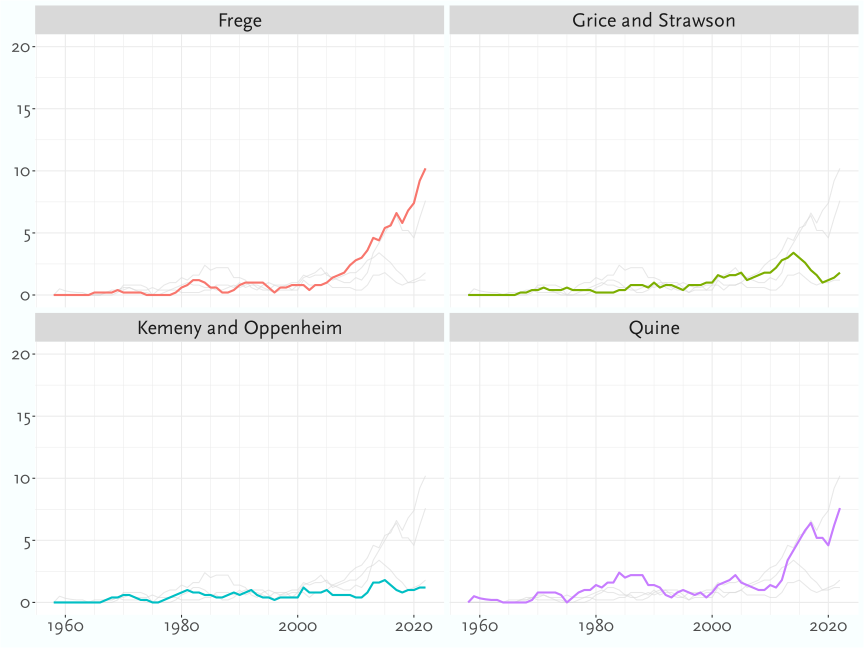
\includegraphics[keepaspectratio]{citations_files/figure-pdf/fig-citation-facet-1956-1.pdf}}

}

\caption{\label{fig-citation-facet-1956}Faceted version of
Figure~\ref{fig-citation-spaghetti-1956}.}

\end{figure}%

\newpage

\subsection{1957}\label{sec-s1957}

\subsubsection*{Widely Cited Articles}\label{widely-cited-articles-1}
\addcontentsline{toc}{subsubsection}{Widely Cited Articles}

\begin{enumerate}
\def\labelenumi{\arabic{enumi}.}
\tightlist
\item
  H. P. Grice (\citeproc{ref-WOSA1957CGZ6000005}{1957}) ``Meaning''
\item
  Zeno Vendler (\citeproc{ref-WOSA1957CCQ4200001}{1957}) ``Verbs and
  Times''
\end{enumerate}

\subsubsection*{Citation Count}\label{sec-count-1957}
\addcontentsline{toc}{subsubsection}{Citation Count}


\begin{longtable}[]{@{}lrrr@{}}

\caption{\label{tbl-citation-count-1957}Citation count for widely cited
articles from 1957.}

\tabularnewline

\toprule\noalign{}
Article & All & Early & Late \\
\midrule\noalign{}
\endhead
\bottomrule\noalign{}
\endlastfoot
Grice (\citeproc{ref-WOSA1957CGZ6000005}{1957})
& 346 & 0 & 176 \\
Vendler (\citeproc{ref-WOSA1957CCQ4200001}{1957})
& 66 & 0 & 49 \\

\end{longtable}

\subsubsection*{Citation Rank}\label{sec-rank-1957}
\addcontentsline{toc}{subsubsection}{Citation Rank}


\begin{longtable}[]{@{}lrrr@{}}

\caption{\label{tbl-citation-rank-1957}Citation rank for widely cited
articles from 1957.}

\tabularnewline

\toprule\noalign{}
Article & Overall & Early & Late \\
\midrule\noalign{}
\endhead
\bottomrule\noalign{}
\endlastfoot
Grice (\citeproc{ref-WOSA1957CGZ6000005}{1957})
& 1 & 70 & 1 \\
Vendler (\citeproc{ref-WOSA1957CCQ4200001}{1957})
& 2 & 70 & 2 \\

\end{longtable}

\subsubsection*{Citation Trends}\label{sec-trends-1957}
\addcontentsline{toc}{subsubsection}{Citation Trends}

\begin{figure}

\centering{

\pandocbounded{\includegraphics[keepaspectratio]{citations_files/figure-pdf/fig-citation-spaghetti-1957-1.pdf}}

}

\caption{\label{fig-citation-spaghetti-1957}Rolling five year average of
citation frequency for widely cited articles from 1957.}

\end{figure}%

\begin{figure}

\centering{

\pandocbounded{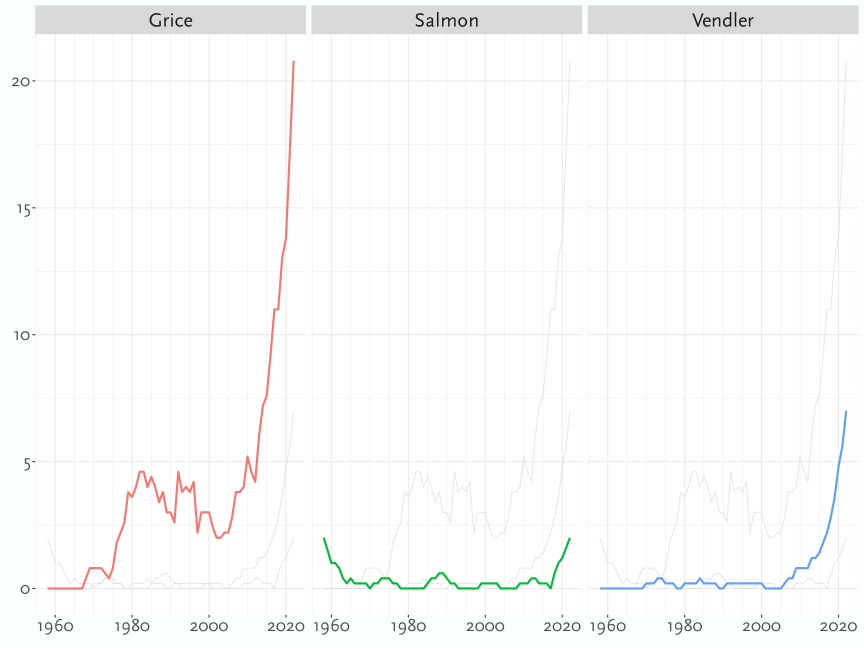
\includegraphics[keepaspectratio]{citations_files/figure-pdf/fig-citation-facet-1957-1.pdf}}

}

\caption{\label{fig-citation-facet-1957}Faceted version of
Figure~\ref{fig-citation-spaghetti-1957}.}

\end{figure}%

\newpage

\subsection{1958}\label{sec-s1958}

\subsubsection*{Widely Cited Articles}\label{widely-cited-articles-2}
\addcontentsline{toc}{subsubsection}{Widely Cited Articles}

\begin{enumerate}
\def\labelenumi{\arabic{enumi}.}
\tightlist
\item
  G. E. M. Anscombe (\citeproc{ref-WOSA1958CDL1000001}{1958}) ``Modern
  Moral Philosophy''
\item
  John R. Searle (\citeproc{ref-WOSA1958CCP4400002}{1958}) ``Proper
  Names''
\item
  John Rawls (\citeproc{ref-WOSA1958CGZ6200002}{1958}) ``Justice as
  Fairness''
\item
  Stuart Hampshire and H. L. A. Hart
  (\citeproc{ref-WOSA1958CGZ9600001}{1958}) ``Decision, Intention and
  Certainty''
\end{enumerate}

\subsubsection*{Citation Count}\label{sec-count-1958}
\addcontentsline{toc}{subsubsection}{Citation Count}


\begin{longtable}[]{@{}lrrr@{}}

\caption{\label{tbl-citation-count-1958}Citation count for widely cited
articles from 1958.}

\tabularnewline

\toprule\noalign{}
Article & All & Early & Late \\
\midrule\noalign{}
\endhead
\bottomrule\noalign{}
\endlastfoot
Anscombe (\citeproc{ref-WOSA1958CDL1000001}{1958})
& 206 & 3 & 116 \\
Searle (\citeproc{ref-WOSA1958CCP4400002}{1958})
& 88 & 2 & 27 \\
Rawls (\citeproc{ref-WOSA1958CGZ6200002}{1958})
& 56 & 7 & 14 \\
Hampshire and Hart (\citeproc{ref-WOSA1958CGZ9600001}{1958})
& 34 & 3 & 15 \\

\end{longtable}

\subsubsection*{Citation Rank}\label{sec-rank-1958}
\addcontentsline{toc}{subsubsection}{Citation Rank}


\begin{longtable}[]{@{}lrrr@{}}

\caption{\label{tbl-citation-rank-1958}Citation rank for widely cited
articles from 1958.}

\tabularnewline

\toprule\noalign{}
Article & Overall & Early & Late \\
\midrule\noalign{}
\endhead
\bottomrule\noalign{}
\endlastfoot
Anscombe (\citeproc{ref-WOSA1958CDL1000001}{1958})
& 1 & 5 & 1 \\
Searle (\citeproc{ref-WOSA1958CCP4400002}{1958})
& 2 & 13 & 2 \\
Rawls (\citeproc{ref-WOSA1958CGZ6200002}{1958})
& 3 & 2 & 5 \\
Hampshire and Hart (\citeproc{ref-WOSA1958CGZ9600001}{1958})
& 4 & 5 & 4 \\

\end{longtable}

\subsubsection*{Citation Trends}\label{sec-trends-1958}
\addcontentsline{toc}{subsubsection}{Citation Trends}

\begin{figure}

\centering{

\pandocbounded{\includegraphics[keepaspectratio]{citations_files/figure-pdf/fig-citation-spaghetti-1958-1.pdf}}

}

\caption{\label{fig-citation-spaghetti-1958}Rolling five year average of
citation frequency for widely cited articles from 1958.}

\end{figure}%

\begin{figure}

\centering{

\pandocbounded{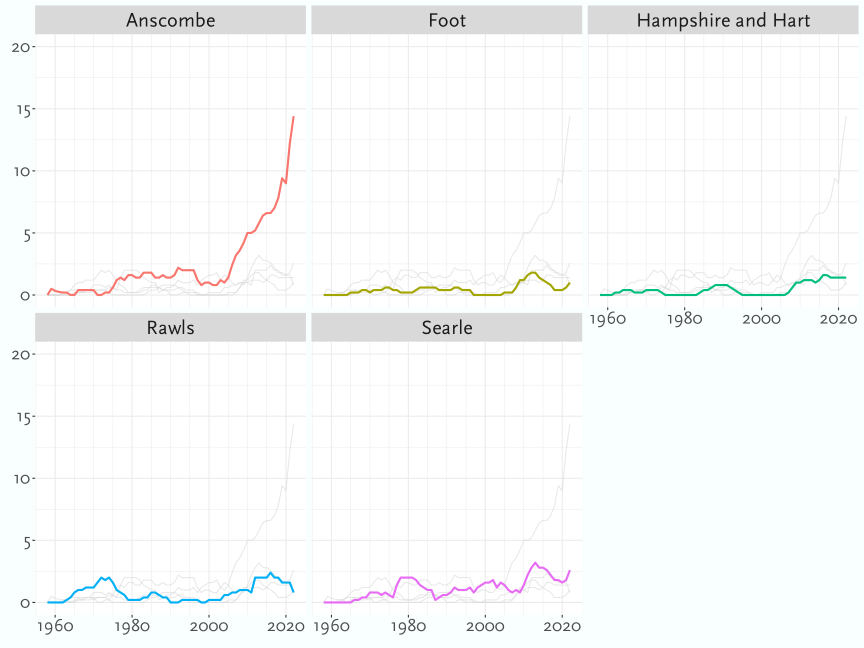
\includegraphics[keepaspectratio]{citations_files/figure-pdf/fig-citation-facet-1958-1.pdf}}

}

\caption{\label{fig-citation-facet-1958}Faceted version of
Figure~\ref{fig-citation-spaghetti-1958}.}

\end{figure}%

\newpage

\subsection{1959}\label{sec-s1959}

\subsubsection*{Widely Cited Articles}\label{widely-cited-articles-3}
\addcontentsline{toc}{subsubsection}{Widely Cited Articles}

\begin{enumerate}
\def\labelenumi{\arabic{enumi}.}
\tightlist
\item
  J. J. C. Smart (\citeproc{ref-WOSA1959CGZ6600001}{1959}) ``Sensations
  and Brain Processes''
\item
  Frank Sibley (\citeproc{ref-WOSA1959CGZ6800001}{1959}) ``Aesthetic
  Concepts''
\item
  A. N. Prior (\citeproc{ref-WOSA1959CDK2600002}{1959}) ``Thank Goodness
  That''s Over''
\item
  Karl R. Popper (\citeproc{ref-WOSA1959CGZ2000003}{1959}) ``The
  Propensity Interpretation of Probability''
\item
  Michael Dummett (\citeproc{ref-WOSA1959CGZ6700003}{1959})
  ``Wittgenstein's Philosophy of Mathematics''
\end{enumerate}

\subsubsection*{Citation Count}\label{sec-count-1959}
\addcontentsline{toc}{subsubsection}{Citation Count}


\begin{longtable}[]{@{}lrrr@{}}

\caption{\label{tbl-citation-count-1959}Citation count for widely cited
articles from 1959.}

\tabularnewline

\toprule\noalign{}
Article & All & Early & Late \\
\midrule\noalign{}
\endhead
\bottomrule\noalign{}
\endlastfoot
Smart (\citeproc{ref-WOSA1959CGZ6600001}{1959})
& 188 & 9 & 87 \\
Sibley (\citeproc{ref-WOSA1959CGZ6800001}{1959})
& 93 & 2 & 56 \\
A. N. Prior (\citeproc{ref-WOSA1959CDK2600002}{1959})
& 90 & 0 & 63 \\
Popper (\citeproc{ref-WOSA1959CGZ2000003}{1959})
& 66 & 2 & 18 \\
Dummett (\citeproc{ref-WOSA1959CGZ6700003}{1959})
& 41 & 4 & 20 \\

\end{longtable}

\subsubsection*{Citation Rank}\label{sec-rank-1959}
\addcontentsline{toc}{subsubsection}{Citation Rank}


\begin{longtable}[]{@{}lrrr@{}}

\caption{\label{tbl-citation-rank-1959}Citation rank for widely cited
articles from 1959.}

\tabularnewline

\toprule\noalign{}
Article & Overall & Early & Late \\
\midrule\noalign{}
\endhead
\bottomrule\noalign{}
\endlastfoot
Smart (\citeproc{ref-WOSA1959CGZ6600001}{1959})
& 1 & 1 & 1 \\
Sibley (\citeproc{ref-WOSA1959CGZ6800001}{1959})
& 2 & 11 & 3 \\
A. N. Prior (\citeproc{ref-WOSA1959CDK2600002}{1959})
& 3 & 76 & 2 \\
Popper (\citeproc{ref-WOSA1959CGZ2000003}{1959})
& 4 & 11 & 5 \\
Dummett (\citeproc{ref-WOSA1959CGZ6700003}{1959})
& 5 & 4 & 4 \\

\end{longtable}

\subsubsection*{Citation Trends}\label{sec-trends-1959}
\addcontentsline{toc}{subsubsection}{Citation Trends}

\begin{figure}

\centering{

\pandocbounded{\includegraphics[keepaspectratio]{citations_files/figure-pdf/fig-citation-spaghetti-1959-1.pdf}}

}

\caption{\label{fig-citation-spaghetti-1959}Rolling five year average of
citation frequency for widely cited articles from 1959.}

\end{figure}%

\begin{figure}

\centering{

\pandocbounded{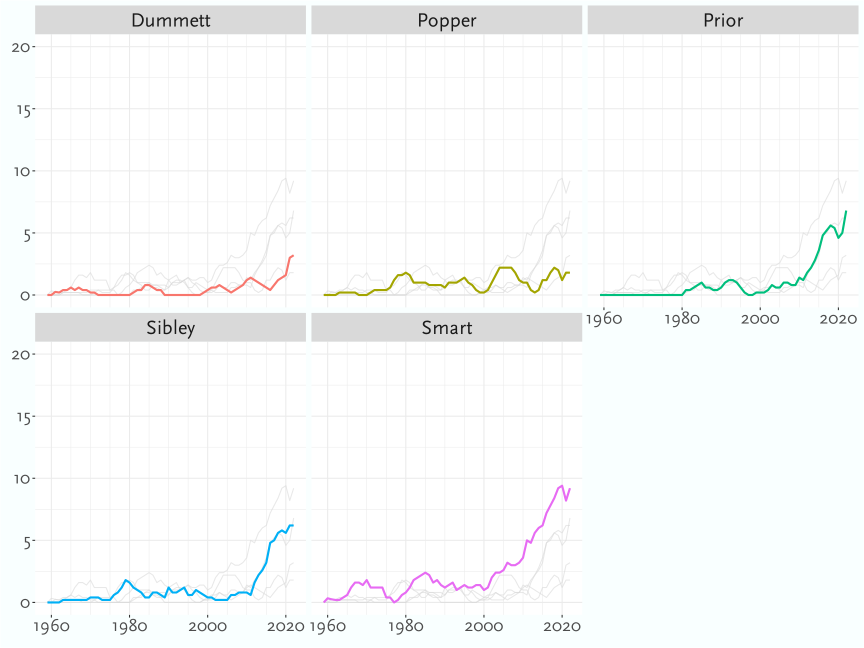
\includegraphics[keepaspectratio]{citations_files/figure-pdf/fig-citation-facet-1959-1.pdf}}

}

\caption{\label{fig-citation-facet-1959}Faceted version of
Figure~\ref{fig-citation-spaghetti-1959}.}

\end{figure}%

\newpage

\subsection{1960}\label{sec-s1960}

\subsubsection*{Widely Cited Articles}\label{widely-cited-articles-4}
\addcontentsline{toc}{subsubsection}{Widely Cited Articles}

\begin{enumerate}
\def\labelenumi{\arabic{enumi}.}
\tightlist
\item
  Peter T. Geach (\citeproc{ref-WOSA1960CCQ4500006}{1960})
  ``Ascriptivism''
\item
  Norman Malcolm (\citeproc{ref-WOSA1960CCQ4400003}{1960}) ``Anselm's
  Ontological Arguments''
\end{enumerate}

\subsubsection*{Citation Count}\label{sec-count-1960}
\addcontentsline{toc}{subsubsection}{Citation Count}


\begin{longtable}[]{@{}lrrr@{}}

\caption{\label{tbl-citation-count-1960}Citation count for widely cited
articles from 1960.}

\tabularnewline

\toprule\noalign{}
Article & All & Early & Late \\
\midrule\noalign{}
\endhead
\bottomrule\noalign{}
\endlastfoot
Geach (\citeproc{ref-WOSA1960CCQ4500006}{1960})
& 70 & 3 & 29 \\
Malcolm (\citeproc{ref-WOSA1960CCQ4400003}{1960})
& 65 & 14 & 18 \\

\end{longtable}

\subsubsection*{Citation Rank}\label{sec-rank-1960}
\addcontentsline{toc}{subsubsection}{Citation Rank}


\begin{longtable}[]{@{}lrrr@{}}

\caption{\label{tbl-citation-rank-1960}Citation rank for widely cited
articles from 1960.}

\tabularnewline

\toprule\noalign{}
Article & Overall & Early & Late \\
\midrule\noalign{}
\endhead
\bottomrule\noalign{}
\endlastfoot
Geach (\citeproc{ref-WOSA1960CCQ4500006}{1960})
& 1 & 5 & 1 \\
Malcolm (\citeproc{ref-WOSA1960CCQ4400003}{1960})
& 2 & 1 & 3 \\

\end{longtable}

\subsubsection*{Citation Trends}\label{sec-trends-1960}
\addcontentsline{toc}{subsubsection}{Citation Trends}

\begin{figure}

\centering{

\pandocbounded{\includegraphics[keepaspectratio]{citations_files/figure-pdf/fig-citation-spaghetti-1960-1.pdf}}

}

\caption{\label{fig-citation-spaghetti-1960}Rolling five year average of
citation frequency for widely cited articles from 1960.}

\end{figure}%

\begin{figure}

\centering{

\pandocbounded{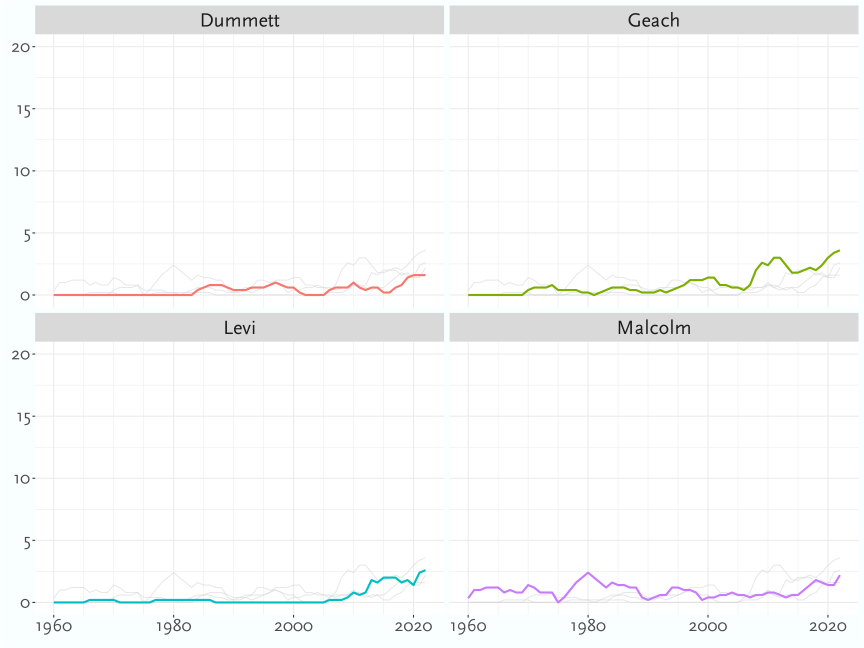
\includegraphics[keepaspectratio]{citations_files/figure-pdf/fig-citation-facet-1960-1.pdf}}

}

\caption{\label{fig-citation-facet-1960}Faceted version of
Figure~\ref{fig-citation-spaghetti-1960}.}

\end{figure}%

\newpage

\subsection{1961}\label{sec-s1961}

\subsubsection*{Widely Cited Articles}\label{widely-cited-articles-5}
\addcontentsline{toc}{subsubsection}{Widely Cited Articles}

\begin{enumerate}
\def\labelenumi{\arabic{enumi}.}
\tightlist
\item
  J. J. C. Smart (\citeproc{ref-WOSA1961CCP4900001}{1961}) ``Free-Will,
  Praise and Blame''
\item
  J. R. Lucas (\citeproc{ref-WOSA1961CDK3300002}{1961}) ``Minds,
  Machines and Gödel''
\item
  I. J. Good (\citeproc{ref-WOSA1961CFT2300005}{1961}) ``A Causal
  Calculus (I)''
\end{enumerate}

\subsubsection*{Citation Count}\label{sec-count-1961}
\addcontentsline{toc}{subsubsection}{Citation Count}


\begin{longtable}[]{@{}lrrr@{}}

\caption{\label{tbl-citation-count-1961}Citation count for widely cited
articles from 1961.}

\tabularnewline

\toprule\noalign{}
Article & All & Early & Late \\
\midrule\noalign{}
\endhead
\bottomrule\noalign{}
\endlastfoot
Smart (\citeproc{ref-WOSA1961CCP4900001}{1961})
& 70 & 3 & 40 \\
Lucas (\citeproc{ref-WOSA1961CDK3300002}{1961})
& 64 & 9 & 17 \\
Good (\citeproc{ref-WOSA1961CFT2300005}{1961})
& 46 & 0 & 16 \\

\end{longtable}

\subsubsection*{Citation Rank}\label{sec-rank-1961}
\addcontentsline{toc}{subsubsection}{Citation Rank}


\begin{longtable}[]{@{}lrrr@{}}

\caption{\label{tbl-citation-rank-1961}Citation rank for widely cited
articles from 1961.}

\tabularnewline

\toprule\noalign{}
Article & Overall & Early & Late \\
\midrule\noalign{}
\endhead
\bottomrule\noalign{}
\endlastfoot
Smart (\citeproc{ref-WOSA1961CCP4900001}{1961})
& 1 & 6 & 1 \\
Lucas (\citeproc{ref-WOSA1961CDK3300002}{1961})
& 2 & 1 & 2 \\
Good (\citeproc{ref-WOSA1961CFT2300005}{1961})
& 3 & 96 & 4 \\

\end{longtable}

\subsubsection*{Citation Trends}\label{sec-trends-1961}
\addcontentsline{toc}{subsubsection}{Citation Trends}

\begin{figure}

\centering{

\pandocbounded{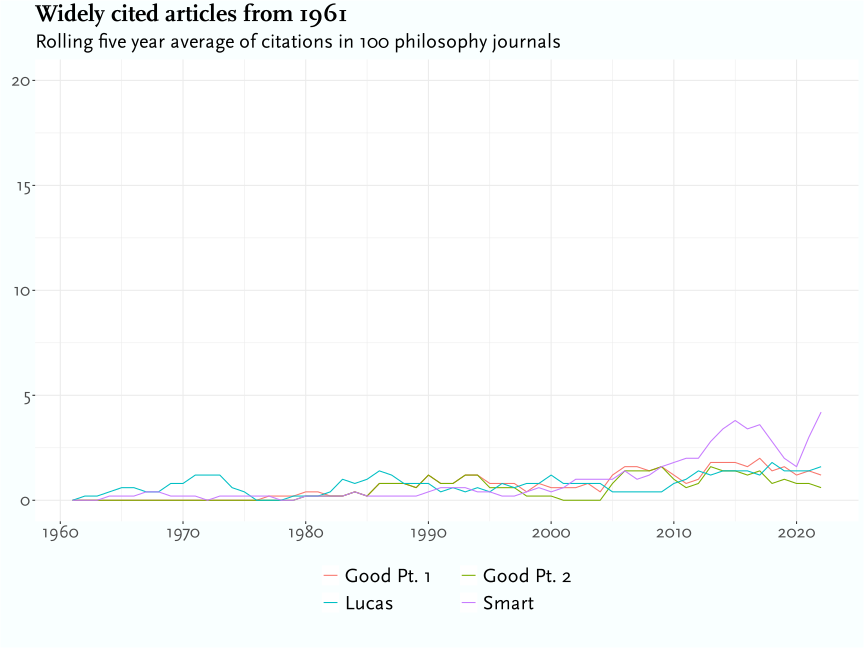
\includegraphics[keepaspectratio]{citations_files/figure-pdf/fig-citation-spaghetti-1961-1.pdf}}

}

\caption{\label{fig-citation-spaghetti-1961}Rolling five year average of
citation frequency for widely cited articles from 1961.}

\end{figure}%

\begin{figure}

\centering{

\pandocbounded{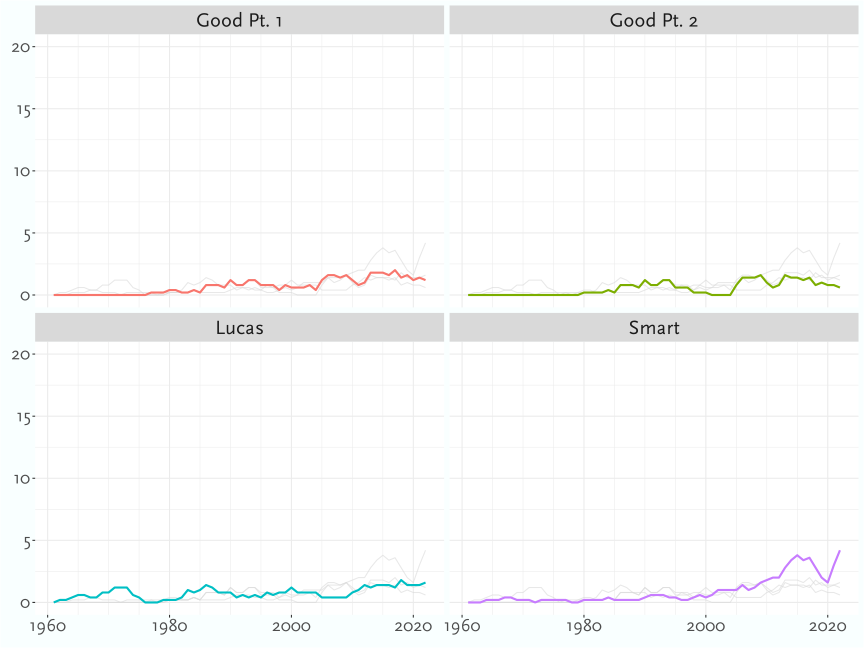
\includegraphics[keepaspectratio]{citations_files/figure-pdf/fig-citation-facet-1961-1.pdf}}

}

\caption{\label{fig-citation-facet-1961}Faceted version of
Figure~\ref{fig-citation-spaghetti-1961}.}

\end{figure}%

\newpage

\subsection{1962}\label{sec-s1962}

\subsubsection*{Widely Cited Articles}\label{widely-cited-articles-6}
\addcontentsline{toc}{subsubsection}{Widely Cited Articles}

\begin{enumerate}
\def\labelenumi{\arabic{enumi}.}
\tightlist
\item
  Hilary Putnam (\citeproc{ref-WOSA1962CET8000004}{1962}) ``It Ain't
  Necessarily So''
\item
  E. J. Lemmon (\citeproc{ref-WOSA1962CGX0600001}{1962}) ``Moral
  Dilemmas''
\item
  John R. Searle (\citeproc{ref-WOSA1962CGX0800001}{1962}) ``Meaning and
  Speech Acts''
\item
  Jaako Hintikka (\citeproc{ref-WOSA1962CGX0500001}{1962}) ``Cogito,
  Ergo Sum: Inference or Performance?''
\end{enumerate}

\subsubsection*{Citation Count}\label{sec-count-1962}
\addcontentsline{toc}{subsubsection}{Citation Count}


\begin{longtable}[]{@{}lrrr@{}}

\caption{\label{tbl-citation-count-1962}Citation count for widely cited
articles from 1962.}

\tabularnewline

\toprule\noalign{}
Article & All & Early & Late \\
\midrule\noalign{}
\endhead
\bottomrule\noalign{}
\endlastfoot
Putnam (\citeproc{ref-WOSA1962CET8000004}{1962})
& 42 & 5 & 22 \\
Lemmon (\citeproc{ref-WOSA1962CGX0600001}{1962})
& 41 & 1 & 13 \\
Searle (\citeproc{ref-WOSA1962CGX0800001}{1962})
& 38 & 2 & 13 \\
Hintikka (\citeproc{ref-WOSA1962CGX0500001}{1962})
& 36 & 3 & 11 \\

\end{longtable}

\subsubsection*{Citation Rank}\label{sec-rank-1962}
\addcontentsline{toc}{subsubsection}{Citation Rank}


\begin{longtable}[]{@{}lrrr@{}}

\caption{\label{tbl-citation-rank-1962}Citation rank for widely cited
articles from 1962.}

\tabularnewline

\toprule\noalign{}
Article & Overall & Early & Late \\
\midrule\noalign{}
\endhead
\bottomrule\noalign{}
\endlastfoot
Putnam (\citeproc{ref-WOSA1962CET8000004}{1962})
& 1 & 4 & 1 \\
Lemmon (\citeproc{ref-WOSA1962CGX0600001}{1962})
& 2 & 28 & 2 \\
Searle (\citeproc{ref-WOSA1962CGX0800001}{1962})
& 3 & 14 & 2 \\
Hintikka (\citeproc{ref-WOSA1962CGX0500001}{1962})
& 4 & 6 & 6 \\

\end{longtable}

\subsubsection*{Citation Trends}\label{sec-trends-1962}
\addcontentsline{toc}{subsubsection}{Citation Trends}

\begin{figure}

\centering{

\pandocbounded{\includegraphics[keepaspectratio]{citations_files/figure-pdf/fig-citation-spaghetti-1962-1.pdf}}

}

\caption{\label{fig-citation-spaghetti-1962}Rolling five year average of
citation frequency for widely cited articles from 1962.}

\end{figure}%

\begin{figure}

\centering{

\pandocbounded{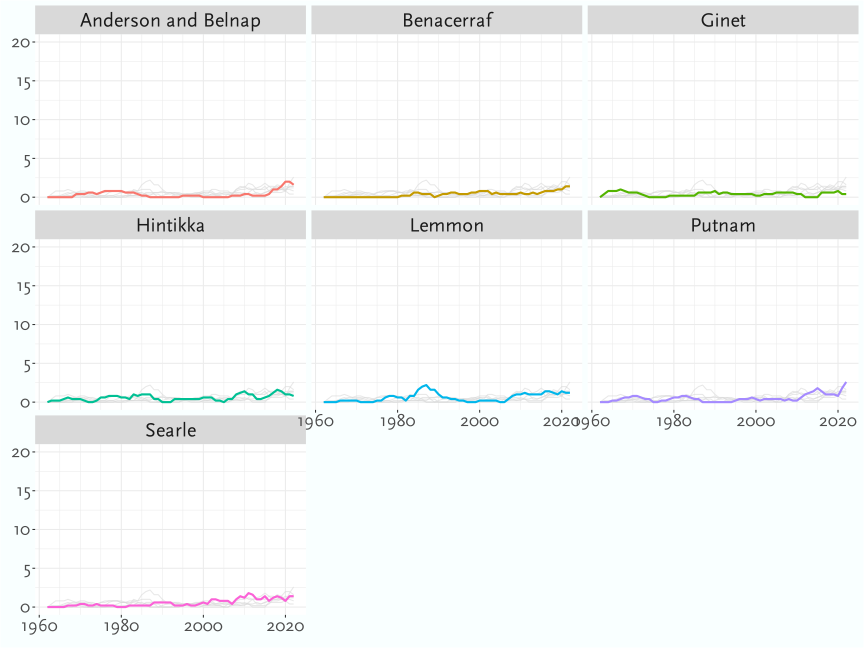
\includegraphics[keepaspectratio]{citations_files/figure-pdf/fig-citation-facet-1962-1.pdf}}

}

\caption{\label{fig-citation-facet-1962}Faceted version of
Figure~\ref{fig-citation-spaghetti-1962}.}

\end{figure}%

\newpage

\subsection{1964}\label{sec-s1964}

\subsubsection*{Widely Cited Articles}\label{widely-cited-articles-7}
\addcontentsline{toc}{subsubsection}{Widely Cited Articles}

\begin{enumerate}
\def\labelenumi{\arabic{enumi}.}
\tightlist
\item
  Arthur Danto (\citeproc{ref-WOSA1964CEU2900005}{1964}) ``The
  Artworld''
\item
  P. F. Strawson (\citeproc{ref-WOSA1964CGZ7200001}{1964}) ``Intention
  and Convention in Speech Acts''
\item
  John R. Searle (\citeproc{ref-WOSA1964CGZ6900003}{1964}) ``How To
  Derive Ought From Is''
\item
  Michael Dummett (\citeproc{ref-WOSA1964CGZ7100003}{1964}) ``Bringing
  About the Past''
\item
  George Dickie (\citeproc{ref-WOSA1964CKG3400005}{1964}) ``The Myth of
  the Aesthetic Attitude''
\end{enumerate}

\subsubsection*{Citation Count}\label{sec-count-1964}
\addcontentsline{toc}{subsubsection}{Citation Count}


\begin{longtable}[]{@{}lrrr@{}}

\caption{\label{tbl-citation-count-1964}Citation count for widely cited
articles from 1964.}

\tabularnewline

\toprule\noalign{}
Article & All & Early & Late \\
\midrule\noalign{}
\endhead
\bottomrule\noalign{}
\endlastfoot
Danto (\citeproc{ref-WOSA1964CEU2900005}{1964})
& 90 & 2 & 35 \\
P. F. Strawson (\citeproc{ref-WOSA1964CGZ7200001}{1964})
& 89 & 3 & 49 \\
Searle (\citeproc{ref-WOSA1964CGZ6900003}{1964})
& 71 & 10 & 28 \\
Dummett (\citeproc{ref-WOSA1964CGZ7100003}{1964})
& 49 & 1 & 20 \\
Dickie (\citeproc{ref-WOSA1964CKG3400005}{1964})
& 48 & 2 & 21 \\

\end{longtable}

\subsubsection*{Citation Rank}\label{sec-rank-1964}
\addcontentsline{toc}{subsubsection}{Citation Rank}


\begin{longtable}[]{@{}lrrr@{}}

\caption{\label{tbl-citation-rank-1964}Citation rank for widely cited
articles from 1964.}

\tabularnewline

\toprule\noalign{}
Article & Overall & Early & Late \\
\midrule\noalign{}
\endhead
\bottomrule\noalign{}
\endlastfoot
Danto (\citeproc{ref-WOSA1964CEU2900005}{1964})
& 1 & 24 & 2 \\
P. F. Strawson (\citeproc{ref-WOSA1964CGZ7200001}{1964})
& 2 & 12 & 1 \\
Searle (\citeproc{ref-WOSA1964CGZ6900003}{1964})
& 3 & 1 & 3 \\
Dummett (\citeproc{ref-WOSA1964CGZ7100003}{1964})
& 4 & 45 & 5 \\
Dickie (\citeproc{ref-WOSA1964CKG3400005}{1964})
& 5 & 24 & 4 \\

\end{longtable}

\subsubsection*{Citation Trends}\label{sec-trends-1964}
\addcontentsline{toc}{subsubsection}{Citation Trends}

\begin{figure}

\centering{

\pandocbounded{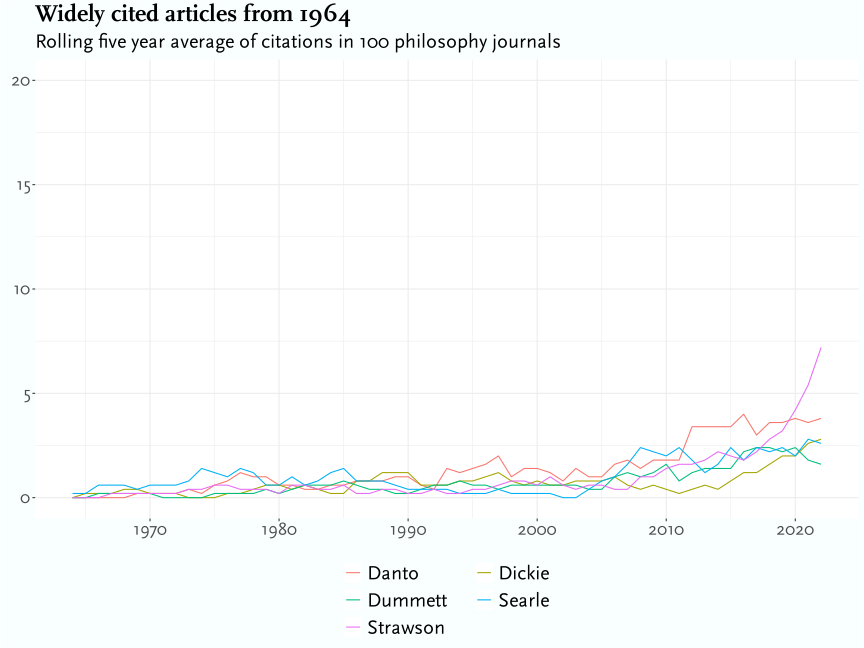
\includegraphics[keepaspectratio]{citations_files/figure-pdf/fig-citation-spaghetti-1964-1.pdf}}

}

\caption{\label{fig-citation-spaghetti-1964}Rolling five year average of
citation frequency for widely cited articles from 1964.}

\end{figure}%

\begin{figure}

\centering{

\pandocbounded{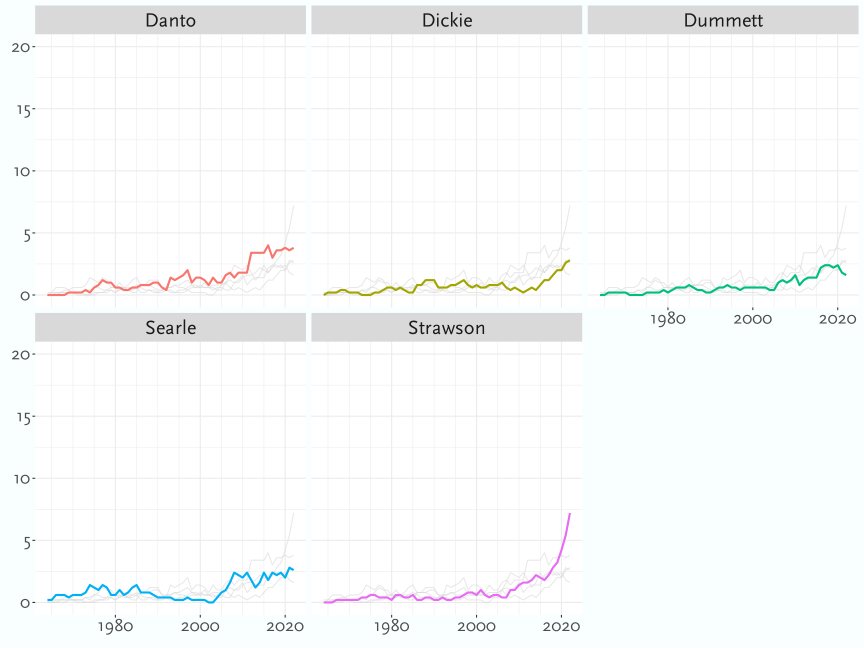
\includegraphics[keepaspectratio]{citations_files/figure-pdf/fig-citation-facet-1964-1.pdf}}

}

\caption{\label{fig-citation-facet-1964}Faceted version of
Figure~\ref{fig-citation-spaghetti-1964}.}

\end{figure}%

\newpage

\subsection{1965}\label{sec-s1965}

\subsubsection*{Widely Cited Articles}\label{widely-cited-articles-8}
\addcontentsline{toc}{subsubsection}{Widely Cited Articles}

\begin{enumerate}
\def\labelenumi{\arabic{enumi}.}
\tightlist
\item
  Paul Benacerraf (\citeproc{ref-WOSA1965CGZ7300005}{1965}) ``What
  Numbers Could Not Be''
\item
  Gilbert Harman (\citeproc{ref-WOSA1965CGZ7300007}{1965}) ``The
  Inference To the Best Explanation''
\item
  Peter T. Geach (\citeproc{ref-WOSA1965CGZ7600002}{1965}) ``Assertion''
\item
  J. L. Mackie (\citeproc{ref-WOSA1965CKS0700001}{1965}) ``Causes and
  Conditions''
\item
  Richard Rorty (\citeproc{ref-WOSA1965CJV5800002}{1965}) ``Mind-Body
  Identity, Privacy, and Categories''
\item
  David L. Hull (\citeproc{ref-WOSA1965CFT3500004}{1965}) ``The Effect
  of Essentialism on Taxonomy: 2000 Years of Stasis (I)''
\item
  Frank Sibley (\citeproc{ref-WOSA1965CGZ7400001}{1965}) ``Aesthetic and
  Non-Aesthetic''
\item
  Joel Feinberg (\citeproc{ref-WOSA1965CJR9200004}{1965}) ``The
  Expressive Function of Punishment''
\end{enumerate}

\subsubsection*{Citation Count}\label{sec-count-1965}
\addcontentsline{toc}{subsubsection}{Citation Count}


\begin{longtable}[]{@{}lrrr@{}}

\caption{\label{tbl-citation-count-1965}Citation count for widely cited
articles from 1965.}

\tabularnewline

\toprule\noalign{}
Article & All & Early & Late \\
\midrule\noalign{}
\endhead
\bottomrule\noalign{}
\endlastfoot
Benacerraf (\citeproc{ref-WOSA1965CGZ7300005}{1965})
& 239 & 5 & 118 \\
Harman (\citeproc{ref-WOSA1965CGZ7300007}{1965})
& 199 & 10 & 87 \\
Geach (\citeproc{ref-WOSA1965CGZ7600002}{1965})
& 167 & 2 & 75 \\
Mackie (\citeproc{ref-WOSA1965CKS0700001}{1965})
& 119 & 9 & 56 \\
Rorty (\citeproc{ref-WOSA1965CJV5800002}{1965})
& 65 & 21 & 13 \\
Hull (\citeproc{ref-WOSA1965CFT3500004}{1965})
& 57 & 0 & 19 \\
Sibley (\citeproc{ref-WOSA1965CGZ7400001}{1965})
& 48 & 1 & 31 \\
Feinberg (\citeproc{ref-WOSA1965CJR9200004}{1965})
& 47 & 2 & 36 \\

\end{longtable}

\subsubsection*{Citation Rank}\label{sec-rank-1965}
\addcontentsline{toc}{subsubsection}{Citation Rank}


\begin{longtable}[]{@{}lrrr@{}}

\caption{\label{tbl-citation-rank-1965}Citation rank for widely cited
articles from 1965.}

\tabularnewline

\toprule\noalign{}
Article & Overall & Early & Late \\
\midrule\noalign{}
\endhead
\bottomrule\noalign{}
\endlastfoot
Benacerraf (\citeproc{ref-WOSA1965CGZ7300005}{1965})
& 1 & 7 & 1 \\
Harman (\citeproc{ref-WOSA1965CGZ7300007}{1965})
& 2 & 2 & 2 \\
Geach (\citeproc{ref-WOSA1965CGZ7600002}{1965})
& 3 & 28 & 3 \\
Mackie (\citeproc{ref-WOSA1965CKS0700001}{1965})
& 4 & 3 & 4 \\
Rorty (\citeproc{ref-WOSA1965CJV5800002}{1965})
& 5 & 1 & 11 \\
Hull (\citeproc{ref-WOSA1965CFT3500004}{1965})
& 6 & 140 & 9 \\
Sibley (\citeproc{ref-WOSA1965CGZ7400001}{1965})
& 8 & 54 & 6 \\
Feinberg (\citeproc{ref-WOSA1965CJR9200004}{1965})
& 10 & 28 & 5 \\

\end{longtable}

\subsubsection*{Citation Trends}\label{sec-trends-1965}
\addcontentsline{toc}{subsubsection}{Citation Trends}

\begin{figure}

\centering{

\pandocbounded{\includegraphics[keepaspectratio]{citations_files/figure-pdf/fig-citation-spaghetti-1965-1.pdf}}

}

\caption{\label{fig-citation-spaghetti-1965}Rolling five year average of
citation frequency for widely cited articles from 1965.}

\end{figure}%

\begin{figure}

\centering{

\pandocbounded{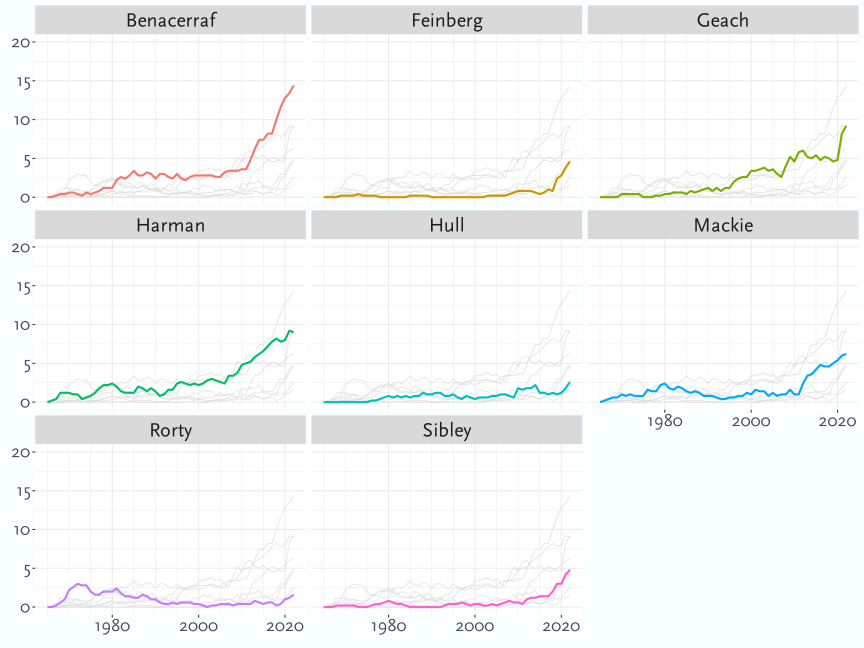
\includegraphics[keepaspectratio]{citations_files/figure-pdf/fig-citation-facet-1965-1.pdf}}

}

\caption{\label{fig-citation-facet-1965}Faceted version of
Figure~\ref{fig-citation-spaghetti-1965}.}

\end{figure}%

\newpage

\subsection{1966}\label{sec-s1966}

\subsubsection*{Widely Cited Articles}\label{widely-cited-articles-9}
\addcontentsline{toc}{subsubsection}{Widely Cited Articles}

\begin{enumerate}
\def\labelenumi{\arabic{enumi}.}
\tightlist
\item
  Keith S. Donnellan (\citeproc{ref-WOSA1966ZC83800001}{1966})
  ``Reference and Definite Descriptions''
\item
  David Lewis (\citeproc{ref-WOSA1966ZC30400002}{1966}) ``An Argument
  for the Identity Theory''
\item
  C. B. Martin and Max Deutscher
  (\citeproc{ref-WOSA1966ZC83700002}{1966}) ``Remembering''
\item
  Bas C. van Fraassen (\citeproc{ref-WOSA1966ZC32000001}{1966})
  ``Singular Terms, Truth-Value Gaps, and Free Logic''
\item
  Jaegwon Kim (\citeproc{ref-WOSA1966ZJ00300003}{1966}) ``On the
  Psycho-Physical Identity Theory''
\item
  Roderick M. Chisholm and Ernest Sosa
  (\citeproc{ref-WOSA1966ZJ00300005}{1966}) ``Logic of Intrinsically
  Better''
\end{enumerate}

\subsubsection*{Citation Count}\label{sec-count-1966}
\addcontentsline{toc}{subsubsection}{Citation Count}


\begin{longtable}[]{@{}lrrr@{}}

\caption{\label{tbl-citation-count-1966}Citation count for widely cited
articles from 1966.}

\tabularnewline

\toprule\noalign{}
Article & All & Early & Late \\
\midrule\noalign{}
\endhead
\bottomrule\noalign{}
\endlastfoot
Donnellan (\citeproc{ref-WOSA1966ZC83800001}{1966})
& 367 & 21 & 121 \\
Lewis (\citeproc{ref-WOSA1966ZC30400002}{1966})
& 146 & 2 & 64 \\
C. B. Martin and Deutscher (\citeproc{ref-WOSA1966ZC83700002}{1966})
& 88 & 3 & 55 \\
Fraassen (\citeproc{ref-WOSA1966ZC32000001}{1966})
& 76 & 8 & 29 \\
Kim (\citeproc{ref-WOSA1966ZJ00300003}{1966})
& 43 & 6 & 9 \\
Chisholm and Sosa (\citeproc{ref-WOSA1966ZJ00300005}{1966})
& 34 & 9 & 13 \\

\end{longtable}

\subsubsection*{Citation Rank}\label{sec-rank-1966}
\addcontentsline{toc}{subsubsection}{Citation Rank}


\begin{longtable}[]{@{}lrrr@{}}

\caption{\label{tbl-citation-rank-1966}Citation rank for widely cited
articles from 1966.}

\tabularnewline

\toprule\noalign{}
Article & Overall & Early & Late \\
\midrule\noalign{}
\endhead
\bottomrule\noalign{}
\endlastfoot
Donnellan (\citeproc{ref-WOSA1966ZC83800001}{1966})
& 1 & 1 & 1 \\
Lewis (\citeproc{ref-WOSA1966ZC30400002}{1966})
& 2 & 32 & 2 \\
C. B. Martin and Deutscher (\citeproc{ref-WOSA1966ZC83700002}{1966})
& 3 & 15 & 3 \\
Fraassen (\citeproc{ref-WOSA1966ZC32000001}{1966})
& 4 & 3 & 4 \\
Kim (\citeproc{ref-WOSA1966ZJ00300003}{1966})
& 5 & 4 & 9 \\
Chisholm and Sosa (\citeproc{ref-WOSA1966ZJ00300005}{1966})
& 6 & 2 & 7 \\

\end{longtable}

\subsubsection*{Citation Trends}\label{sec-trends-1966}
\addcontentsline{toc}{subsubsection}{Citation Trends}

\begin{figure}

\centering{

\pandocbounded{\includegraphics[keepaspectratio]{citations_files/figure-pdf/fig-citation-spaghetti-1966-1.pdf}}

}

\caption{\label{fig-citation-spaghetti-1966}Rolling five year average of
citation frequency for widely cited articles from 1966.}

\end{figure}%

\begin{figure}

\centering{

\pandocbounded{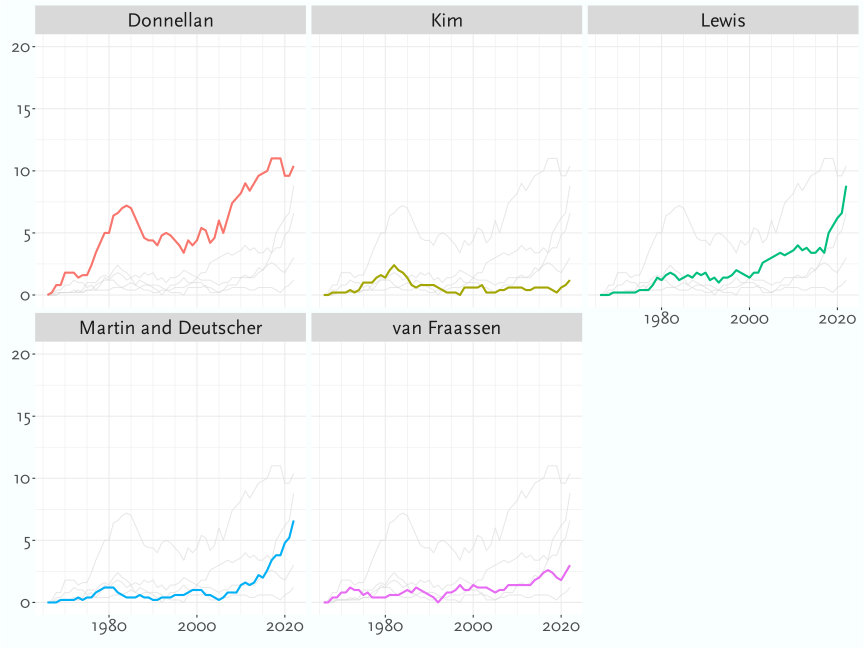
\includegraphics[keepaspectratio]{citations_files/figure-pdf/fig-citation-facet-1966-1.pdf}}

}

\caption{\label{fig-citation-facet-1966}Faceted version of
Figure~\ref{fig-citation-spaghetti-1966}.}

\end{figure}%

\newpage

\subsection{1967}\label{sec-s1967}

\subsubsection*{Widely Cited Articles}\label{widely-cited-articles-10}
\addcontentsline{toc}{subsubsection}{Widely Cited Articles}

\begin{enumerate}
\def\labelenumi{\arabic{enumi}.}
\tightlist
\item
  Donald Davidson (\citeproc{ref-WOSA1967ZP14500007}{1967b}) ``Truth and
  Meaning''
\item
  Alvin I. Goldman (\citeproc{ref-WOSA1967ZC33900001}{1967}) ``A Causal
  Theory of Knowing''
\item
  Donald Davidson (\citeproc{ref-WOSA1967ZC34800001}{1967a}) ``Causal
  Relations''
\item
  Hector-Neri Castañeda (\citeproc{ref-WOSA1967ZH25100001}{1967})
  ``Indicators and Quasi-Indicators''
\item
  Kenneth F. Schaffner (\citeproc{ref-WOSA1967ZC89200003}{1967})
  ``Approaches To Reduction''
\item
  Hilary Putnam (\citeproc{ref-WOSA1967ZC33500002}{1967}) ``Time and
  Physical Geometry''
\item
  Ian Hacking (\citeproc{ref-WOSA1967ZC89400002}{1967b}) ``Slightly More
  Realistic Personal Probability''
\item
  Ian Hacking (\citeproc{ref-WOSA1967ZC84100001}{1967a}) ``Possibility''
\end{enumerate}

\subsubsection*{Citation Count}\label{sec-count-1967}
\addcontentsline{toc}{subsubsection}{Citation Count}


\begin{longtable}[]{@{}lrrr@{}}

\caption{\label{tbl-citation-count-1967}Citation count for widely cited
articles from 1967.}

\tabularnewline

\toprule\noalign{}
Article & All & Early & Late \\
\midrule\noalign{}
\endhead
\bottomrule\noalign{}
\endlastfoot
Davidson (\citeproc{ref-WOSA1967ZP14500007}{1967b})
& 166 & 16 & 54 \\
Goldman (\citeproc{ref-WOSA1967ZC33900001}{1967})
& 164 & 16 & 80 \\
Davidson (\citeproc{ref-WOSA1967ZC34800001}{1967a})
& 134 & 17 & 45 \\
Castañeda (\citeproc{ref-WOSA1967ZH25100001}{1967})
& 104 & 12 & 20 \\
Schaffner (\citeproc{ref-WOSA1967ZC89200003}{1967})
& 103 & 6 & 22 \\
Putnam (\citeproc{ref-WOSA1967ZC33500002}{1967})
& 91 & 4 & 47 \\
Hacking (\citeproc{ref-WOSA1967ZC89400002}{1967b})
& 69 & 4 & 29 \\
Hacking (\citeproc{ref-WOSA1967ZC84100001}{1967a})
& 63 & 3 & 36 \\

\end{longtable}

\subsubsection*{Citation Rank}\label{sec-rank-1967}
\addcontentsline{toc}{subsubsection}{Citation Rank}


\begin{longtable}[]{@{}lrrr@{}}

\caption{\label{tbl-citation-rank-1967}Citation rank for widely cited
articles from 1967.}

\tabularnewline

\toprule\noalign{}
Article & Overall & Early & Late \\
\midrule\noalign{}
\endhead
\bottomrule\noalign{}
\endlastfoot
Davidson (\citeproc{ref-WOSA1967ZP14500007}{1967b})
& 1 & 2 & 2 \\
Goldman (\citeproc{ref-WOSA1967ZC33900001}{1967})
& 2 & 2 & 1 \\
Davidson (\citeproc{ref-WOSA1967ZC34800001}{1967a})
& 3 & 1 & 4 \\
Castañeda (\citeproc{ref-WOSA1967ZH25100001}{1967})
& 4 & 4 & 12 \\
Schaffner (\citeproc{ref-WOSA1967ZC89200003}{1967})
& 5 & 9 & 10 \\
Putnam (\citeproc{ref-WOSA1967ZC33500002}{1967})
& 6 & 16 & 3 \\
Hacking (\citeproc{ref-WOSA1967ZC89400002}{1967b})
& 7 & 16 & 6 \\
Hacking (\citeproc{ref-WOSA1967ZC84100001}{1967a})
& 8 & 28 & 5 \\

\end{longtable}

\subsubsection*{Citation Trends}\label{sec-trends-1967}
\addcontentsline{toc}{subsubsection}{Citation Trends}

\begin{figure}

\centering{

\pandocbounded{\includegraphics[keepaspectratio]{citations_files/figure-pdf/fig-citation-spaghetti-1967-1.pdf}}

}

\caption{\label{fig-citation-spaghetti-1967}Rolling five year average of
citation frequency for widely cited articles from 1967.}

\end{figure}%

\begin{figure}

\centering{

\pandocbounded{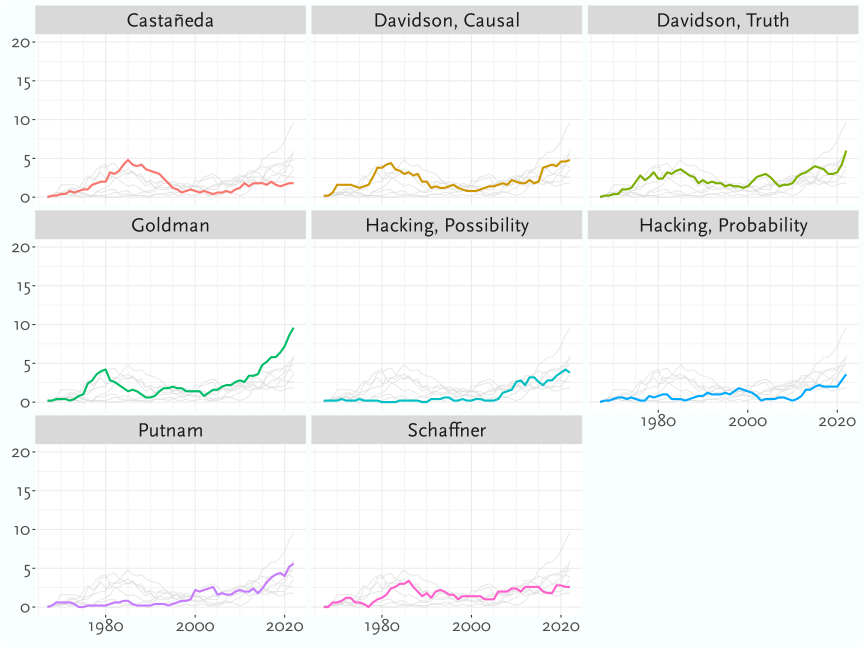
\includegraphics[keepaspectratio]{citations_files/figure-pdf/fig-citation-facet-1967-1.pdf}}

}

\caption{\label{fig-citation-facet-1967}Faceted version of
Figure~\ref{fig-citation-spaghetti-1967}.}

\end{figure}%

\newpage

\subsection{1968}\label{sec-s1968}

\subsubsection*{Widely Cited Articles}\label{widely-cited-articles-11}
\addcontentsline{toc}{subsubsection}{Widely Cited Articles}

\begin{enumerate}
\def\labelenumi{\arabic{enumi}.}
\tightlist
\item
  David Lewis (\citeproc{ref-WOSA1968ZE29500001}{1968}) ``Counterpart
  Theory and Quantified Modal Logic''
\item
  Sydney Shoemaker (\citeproc{ref-WOSA1968ZE30900001}{1968})
  ``Self-Reference and Self-Awareness''
\item
  Barry Stroud (\citeproc{ref-WOSA1968ZE29900001}{1968})
  ``Transcendental Arguments''
\item
  Peter Unger (\citeproc{ref-WOSA1968ZE29600001}{1968}) ``An Analysis of
  Factual Knowledge''
\item
  Herbert Morris (\citeproc{ref-WOSA1968ZL99200001}{1968}) ``Persons and
  Punishment''
\item
  Willard van Orman Quine (\citeproc{ref-WOSA1968ZE29700001}{1968})
  ``Ontological Relativity''
\item
  Bas C. van Fraassen (\citeproc{ref-WOSA1968ZE29500003}{1968})
  ``Presupposition, Implication, and Self-Reference''
\item
  Gilbert Harman (\citeproc{ref-WOSA1968ZB45300003}{1968}) ``Knowledge,
  Inference, and Explanation''
\end{enumerate}

\subsubsection*{Citation Count}\label{sec-count-1968}
\addcontentsline{toc}{subsubsection}{Citation Count}


\begin{longtable}[]{@{}lrrr@{}}

\caption{\label{tbl-citation-count-1968}Citation count for widely cited
articles from 1968.}

\tabularnewline

\toprule\noalign{}
Article & All & Early & Late \\
\midrule\noalign{}
\endhead
\bottomrule\noalign{}
\endlastfoot
Lewis (\citeproc{ref-WOSA1968ZE29500001}{1968})
& 224 & 8 & 99 \\
Shoemaker (\citeproc{ref-WOSA1968ZE30900001}{1968})
& 118 & 1 & 76 \\
Stroud (\citeproc{ref-WOSA1968ZE29900001}{1968})
& 102 & 9 & 40 \\
Unger (\citeproc{ref-WOSA1968ZE29600001}{1968})
& 90 & 10 & 49 \\
Morris (\citeproc{ref-WOSA1968ZL99200001}{1968})
& 85 & 3 & 26 \\
Orman Quine (\citeproc{ref-WOSA1968ZE29700001}{1968})
& 56 & 4 & 33 \\
Fraassen (\citeproc{ref-WOSA1968ZE29500003}{1968})
& 53 & 16 & 10 \\
Harman (\citeproc{ref-WOSA1968ZB45300003}{1968})
& 45 & 12 & 14 \\

\end{longtable}

\subsubsection*{Citation Rank}\label{sec-rank-1968}
\addcontentsline{toc}{subsubsection}{Citation Rank}


\begin{longtable}[]{@{}lrrr@{}}

\caption{\label{tbl-citation-rank-1968}Citation rank for widely cited
articles from 1968.}

\tabularnewline

\toprule\noalign{}
Article & Overall & Early & Late \\
\midrule\noalign{}
\endhead
\bottomrule\noalign{}
\endlastfoot
Lewis (\citeproc{ref-WOSA1968ZE29500001}{1968})
& 1 & 6 & 1 \\
Shoemaker (\citeproc{ref-WOSA1968ZE30900001}{1968})
& 2 & 63 & 2 \\
Stroud (\citeproc{ref-WOSA1968ZE29900001}{1968})
& 3 & 4 & 4 \\
Unger (\citeproc{ref-WOSA1968ZE29600001}{1968})
& 4 & 3 & 3 \\
Morris (\citeproc{ref-WOSA1968ZL99200001}{1968})
& 5 & 22 & 7 \\
Orman Quine (\citeproc{ref-WOSA1968ZE29700001}{1968})
& 7 & 15 & 5 \\
Fraassen (\citeproc{ref-WOSA1968ZE29500003}{1968})
& 8 & 1 & 15 \\
Harman (\citeproc{ref-WOSA1968ZB45300003}{1968})
& 10 & 2 & 13 \\

\end{longtable}

\subsubsection*{Citation Trends}\label{sec-trends-1968}
\addcontentsline{toc}{subsubsection}{Citation Trends}

\begin{figure}

\centering{

\pandocbounded{\includegraphics[keepaspectratio]{citations_files/figure-pdf/fig-citation-spaghetti-1968-1.pdf}}

}

\caption{\label{fig-citation-spaghetti-1968}Rolling five year average of
citation frequency for widely cited articles from 1968.}

\end{figure}%

\begin{figure}

\centering{

\pandocbounded{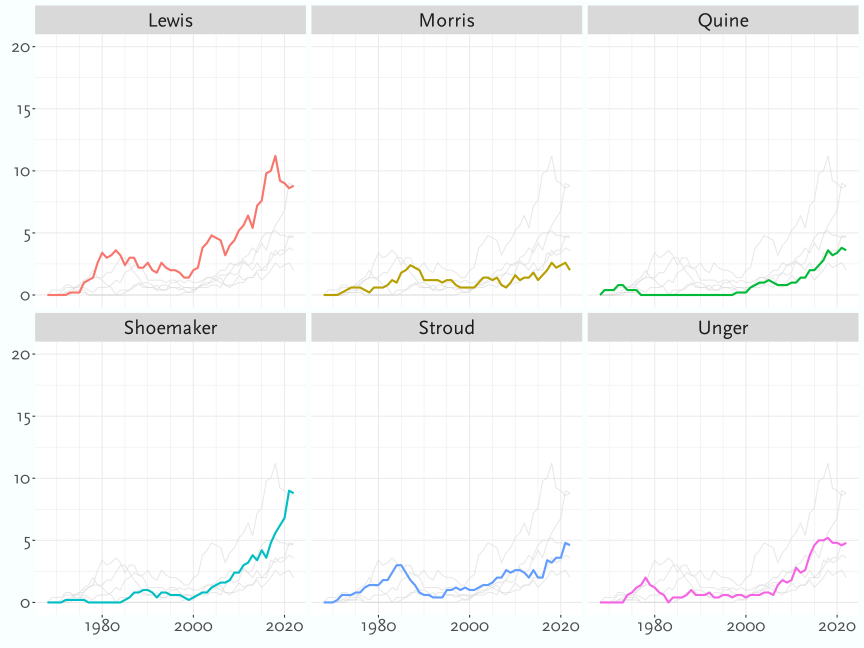
\includegraphics[keepaspectratio]{citations_files/figure-pdf/fig-citation-facet-1968-1.pdf}}

}

\caption{\label{fig-citation-facet-1968}Faceted version of
Figure~\ref{fig-citation-spaghetti-1968}.}

\end{figure}%

\newpage

\subsection{1969}\label{sec-s1969}

\subsubsection*{Widely Cited Articles}\label{widely-cited-articles-12}
\addcontentsline{toc}{subsubsection}{Widely Cited Articles}

\begin{enumerate}
\def\labelenumi{\arabic{enumi}.}
\tightlist
\item
  Harry G. Frankfurt (\citeproc{ref-WOSA1969Y444700002}{1969})
  ``Alternate Possibilities and Moral Responsibility''
\item
  H. P. Grice (\citeproc{ref-WOSA1969Y406100001}{1969}) ``Utterer's
  Meaning and Intentions''
\item
  Keith Lehrer and Thomas Paxson Jr.
  (\citeproc{ref-WOSA1969Y443200001}{1969}) ``Knowledge: Undefeated
  Justified True Belief''
\item
  Bas C. van Fraassen (\citeproc{ref-WOSA1969Y443900001}{1969}) ``Facts
  and Tautological Entailments''
\item
  J. A. Goguen (\citeproc{ref-WOSA1969ZP70500001}{1969}) ``The Logic of
  Inexact Concepts''
\end{enumerate}

\subsubsection*{Citation Count}\label{sec-count-1969}
\addcontentsline{toc}{subsubsection}{Citation Count}


\begin{longtable}[]{@{}lrrr@{}}

\caption{\label{tbl-citation-count-1969}Citation count for widely cited
articles from 1969.}

\tabularnewline

\toprule\noalign{}
Article & All & Early & Late \\
\midrule\noalign{}
\endhead
\bottomrule\noalign{}
\endlastfoot
Frankfurt (\citeproc{ref-WOSA1969Y444700002}{1969})
& 513 & 4 & 279 \\
Grice (\citeproc{ref-WOSA1969Y406100001}{1969})
& 113 & 10 & 40 \\
Lehrer and Jr. (\citeproc{ref-WOSA1969Y443200001}{1969})
& 100 & 12 & 44 \\
Fraassen (\citeproc{ref-WOSA1969Y443900001}{1969})
& 54 & 4 & 32 \\
Goguen (\citeproc{ref-WOSA1969ZP70500001}{1969})
& 51 & 2 & 11 \\

\end{longtable}

\subsubsection*{Citation Rank}\label{sec-rank-1969}
\addcontentsline{toc}{subsubsection}{Citation Rank}


\begin{longtable}[]{@{}lrrr@{}}

\caption{\label{tbl-citation-rank-1969}Citation rank for widely cited
articles from 1969.}

\tabularnewline

\toprule\noalign{}
Article & Overall & Early & Late \\
\midrule\noalign{}
\endhead
\bottomrule\noalign{}
\endlastfoot
Frankfurt (\citeproc{ref-WOSA1969Y444700002}{1969})
& 1 & 14 & 1 \\
Grice (\citeproc{ref-WOSA1969Y406100001}{1969})
& 2 & 3 & 3 \\
Lehrer and Jr. (\citeproc{ref-WOSA1969Y443200001}{1969})
& 3 & 2 & 2 \\
Fraassen (\citeproc{ref-WOSA1969Y443900001}{1969})
& 4 & 14 & 4 \\
Goguen (\citeproc{ref-WOSA1969ZP70500001}{1969})
& 5 & 45 & 10 \\

\end{longtable}

\subsubsection*{Citation Trends}\label{sec-trends-1969}
\addcontentsline{toc}{subsubsection}{Citation Trends}

\begin{figure}

\centering{

\pandocbounded{\includegraphics[keepaspectratio]{citations_files/figure-pdf/fig-citation-spaghetti-1969-1.pdf}}

}

\caption{\label{fig-citation-spaghetti-1969}Rolling five year average of
citation frequency for widely cited articles from 1969.}

\end{figure}%

\begin{figure}

\centering{

\pandocbounded{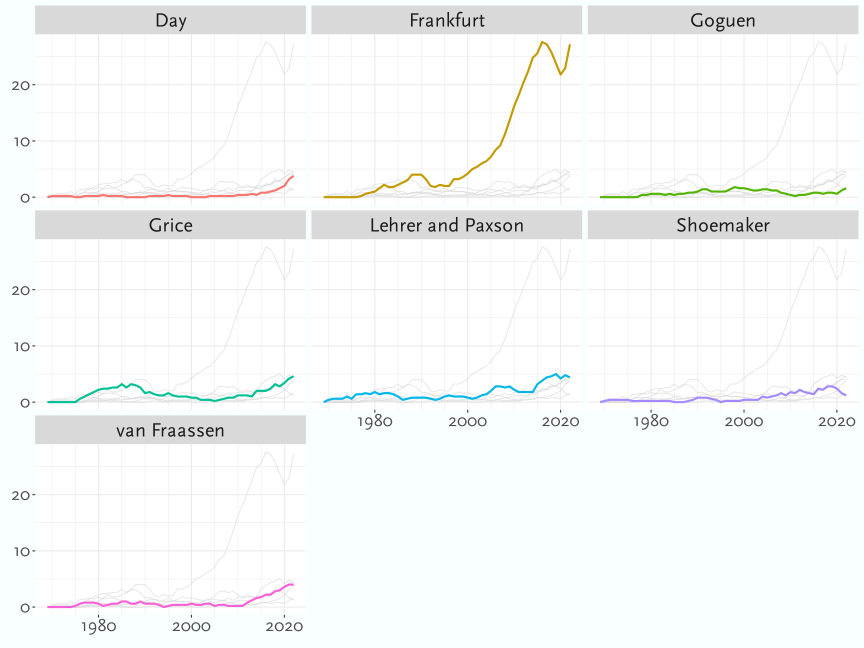
\includegraphics[keepaspectratio]{citations_files/figure-pdf/fig-citation-facet-1969-1.pdf}}

}

\caption{\label{fig-citation-facet-1969}Faceted version of
Figure~\ref{fig-citation-spaghetti-1969}.}

\end{figure}%

\newpage

\subsection{1970}\label{sec-s1970}

\subsubsection*{Widely Cited Articles}\label{widely-cited-articles-13}
\addcontentsline{toc}{subsubsection}{Widely Cited Articles}

\begin{enumerate}
\def\labelenumi{\arabic{enumi}.}
\tightlist
\item
  Fred Dretske (\citeproc{ref-WOSA1970ZE33800001}{1970}) ``Epistemic
  Operators''
\item
  David Lewis (\citeproc{ref-WOSA1970ZE32700001}{1970}) ``How To Define
  Theoretical Terms''
\item
  Kendall L. Walton (\citeproc{ref-WOSA1970Y384700002}{1970})
  ``Categories of Art''
\item
  Robert Stalnaker (\citeproc{ref-WOSA1970G279500005}{1970})
  ``Probability and Conditionals''
\item
  Sydney Shoemaker (\citeproc{ref-WOSA1970Y183500001}{1970}) ``Persons
  and Their Pasts''
\item
  Willard van Orman Quine (\citeproc{ref-WOSA1970ZE32000003}{1970}) ``On
  the Reasons for Indeterminacy of Translation''
\item
  Bas C. van Fraassen (\citeproc{ref-WOSA1970H499300001}{1970}) ``On
  Extension of Beths Semantics of Physical Theories''
\item
  Richard Rorty (\citeproc{ref-WOSA1970ZE32600001}{1970})
  ``Incorrigibility as Mark of Mental''
\end{enumerate}

\subsubsection*{Citation Count}\label{sec-count-1970}
\addcontentsline{toc}{subsubsection}{Citation Count}


\begin{longtable}[]{@{}lrrr@{}}

\caption{\label{tbl-citation-count-1970}Citation count for widely cited
articles from 1970.}

\tabularnewline

\toprule\noalign{}
Article & All & Early & Late \\
\midrule\noalign{}
\endhead
\bottomrule\noalign{}
\endlastfoot
Dretske (\citeproc{ref-WOSA1970ZE33800001}{1970})
& 337 & 3 & 162 \\
Lewis (\citeproc{ref-WOSA1970ZE32700001}{1970})
& 241 & 5 & 114 \\
Walton (\citeproc{ref-WOSA1970Y384700002}{1970})
& 174 & 4 & 97 \\
Stalnaker (\citeproc{ref-WOSA1970G279500005}{1970})
& 96 & 6 & 48 \\
Shoemaker (\citeproc{ref-WOSA1970Y183500001}{1970})
& 95 & 3 & 47 \\
Orman Quine (\citeproc{ref-WOSA1970ZE32000003}{1970})
& 68 & 16 & 13 \\
Fraassen (\citeproc{ref-WOSA1970H499300001}{1970})
& 52 & 8 & 17 \\
Rorty (\citeproc{ref-WOSA1970ZE32600001}{1970})
& 35 & 11 & 5 \\

\end{longtable}

\subsubsection*{Citation Rank}\label{sec-rank-1970}
\addcontentsline{toc}{subsubsection}{Citation Rank}


\begin{longtable}[]{@{}lrrr@{}}

\caption{\label{tbl-citation-rank-1970}Citation rank for widely cited
articles from 1970.}

\tabularnewline

\toprule\noalign{}
Article & Overall & Early & Late \\
\midrule\noalign{}
\endhead
\bottomrule\noalign{}
\endlastfoot
Dretske (\citeproc{ref-WOSA1970ZE33800001}{1970})
& 1 & 38 & 1 \\
Lewis (\citeproc{ref-WOSA1970ZE32700001}{1970})
& 2 & 17 & 2 \\
Walton (\citeproc{ref-WOSA1970Y384700002}{1970})
& 3 & 26 & 3 \\
Stalnaker (\citeproc{ref-WOSA1970G279500005}{1970})
& 4 & 11 & 4 \\
Shoemaker (\citeproc{ref-WOSA1970Y183500001}{1970})
& 5 & 38 & 5 \\
Orman Quine (\citeproc{ref-WOSA1970ZE32000003}{1970})
& 7 & 1 & 13 \\
Fraassen (\citeproc{ref-WOSA1970H499300001}{1970})
& 9 & 5 & 10 \\
Rorty (\citeproc{ref-WOSA1970ZE32600001}{1970})
& 14 & 2 & 25 \\

\end{longtable}

\subsubsection*{Citation Trends}\label{sec-trends-1970}
\addcontentsline{toc}{subsubsection}{Citation Trends}

\begin{figure}

\centering{

\pandocbounded{\includegraphics[keepaspectratio]{citations_files/figure-pdf/fig-citation-spaghetti-1970-1.pdf}}

}

\caption{\label{fig-citation-spaghetti-1970}Rolling five year average of
citation frequency for widely cited articles from 1970.}

\end{figure}%

\begin{figure}

\centering{

\pandocbounded{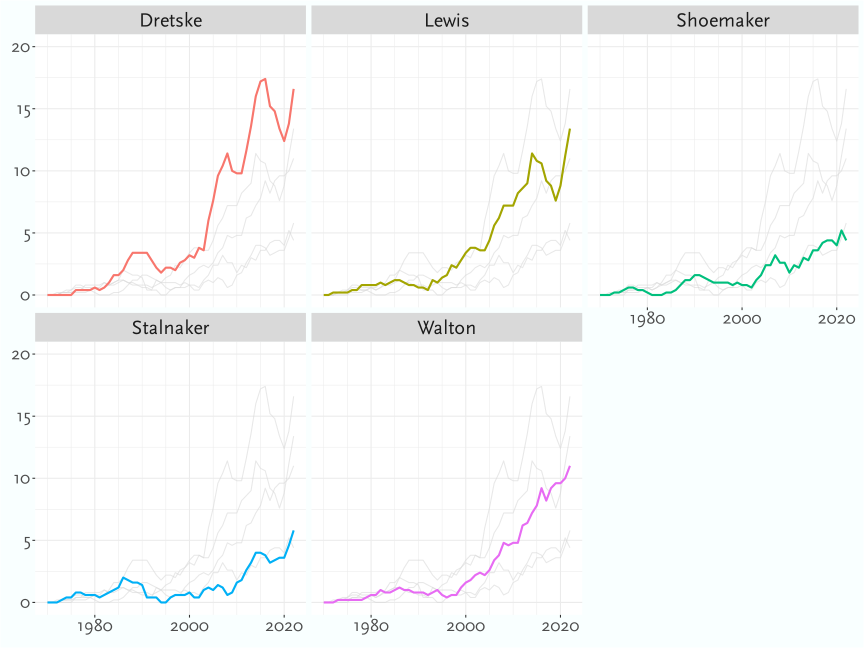
\includegraphics[keepaspectratio]{citations_files/figure-pdf/fig-citation-facet-1970-1.pdf}}

}

\caption{\label{fig-citation-facet-1970}Faceted version of
Figure~\ref{fig-citation-spaghetti-1970}.}

\end{figure}%

\newpage

\subsection{1971}\label{sec-s1971}

\subsubsection*{Widely Cited Articles}\label{widely-cited-articles-14}
\addcontentsline{toc}{subsubsection}{Widely Cited Articles}

\begin{enumerate}
\def\labelenumi{\arabic{enumi}.}
\tightlist
\item
  Harry G. Frankfurt (\citeproc{ref-10.2307_2024717}{1971}) ``Freedom of
  the Will and the Concept of a Person''
\item
  Judith Jarvis Thomson (\citeproc{ref-WOSA1971Y116900003}{1971}) ``A
  Defense of Abortion''
\item
  Derek Parfit (\citeproc{ref-WOSA1971Y036400001}{1971}) ``Personal
  Identity''
\item
  D. C. Dennett (\citeproc{ref-10.2307_2025382}{1971}) ``Intentional
  Systems''
\item
  David Lewis (\citeproc{ref-10.2307_2024902}{1971}) ``Counterparts of
  Persons and Their Bodies''
\item
  George Boolos (\citeproc{ref-10.2307_2025204}{1971}) ``The Iterative
  Conception of Set''
\item
  William P. Alston (\citeproc{ref-WOSA1971Y185900002}{1971})
  ``Varieties of Privileged Access''
\item
  R. Eugene Bales (\citeproc{ref-WOSA1971Y185900004}{1971})
  ``Act-Utilitarianism: Account of Right-Making Characteristics or
  Decision-Making Procedure''
\item
  Alvin I. Goldman (\citeproc{ref-10.2307_2024949}{1971}) ``The
  Individuation of Action''
\end{enumerate}

\subsubsection*{Citation Count}\label{sec-count-1971}
\addcontentsline{toc}{subsubsection}{Citation Count}


\begin{longtable}[]{@{}lrrr@{}}

\caption{\label{tbl-citation-count-1971}Citation count for widely cited
articles from 1971.}

\tabularnewline

\toprule\noalign{}
Article & All & Early & Late \\
\midrule\noalign{}
\endhead
\bottomrule\noalign{}
\endlastfoot
Frankfurt (\citeproc{ref-10.2307_2024717}{1971})
& 563 & 34 & 247 \\
Thomson (\citeproc{ref-WOSA1971Y116900003}{1971})
& 250 & 20 & 121 \\
Parfit (\citeproc{ref-WOSA1971Y036400001}{1971})
& 148 & 16 & 61 \\
D. C. Dennett (\citeproc{ref-10.2307_2025382}{1971})
& 126 & 18 & 41 \\
Lewis (\citeproc{ref-10.2307_2024902}{1971})
& 112 & 9 & 48 \\
Boolos (\citeproc{ref-10.2307_2025204}{1971})
& 91 & 4 & 48 \\
Alston (\citeproc{ref-WOSA1971Y185900002}{1971})
& 52 & 5 & 18 \\
Bales (\citeproc{ref-WOSA1971Y185900004}{1971})
& 52 & 1 & 29 \\
Goldman (\citeproc{ref-10.2307_2024949}{1971})
& 44 & 17 & 9 \\

\end{longtable}

\subsubsection*{Citation Rank}\label{sec-rank-1971}
\addcontentsline{toc}{subsubsection}{Citation Rank}


\begin{longtable}[]{@{}lrrr@{}}

\caption{\label{tbl-citation-rank-1971}Citation rank for widely cited
articles from 1971.}

\tabularnewline

\toprule\noalign{}
Article & Overall & Early & Late \\
\midrule\noalign{}
\endhead
\bottomrule\noalign{}
\endlastfoot
Frankfurt (\citeproc{ref-10.2307_2024717}{1971})
& 1 & 1 & 1 \\
Thomson (\citeproc{ref-WOSA1971Y116900003}{1971})
& 2 & 2 & 2 \\
Parfit (\citeproc{ref-WOSA1971Y036400001}{1971})
& 3 & 5 & 3 \\
D. C. Dennett (\citeproc{ref-10.2307_2025382}{1971})
& 4 & 3 & 6 \\
Lewis (\citeproc{ref-10.2307_2024902}{1971})
& 5 & 9 & 4 \\
Boolos (\citeproc{ref-10.2307_2025204}{1971})
& 6 & 32 & 4 \\
Alston (\citeproc{ref-WOSA1971Y185900002}{1971})
& 7 & 19 & 11 \\
Bales (\citeproc{ref-WOSA1971Y185900004}{1971})
& 7 & 112 & 8 \\
Goldman (\citeproc{ref-10.2307_2024949}{1971})
& 10 & 4 & 16 \\

\end{longtable}

\subsubsection*{Citation Trends}\label{sec-trends-1971}
\addcontentsline{toc}{subsubsection}{Citation Trends}

\begin{figure}

\centering{

\pandocbounded{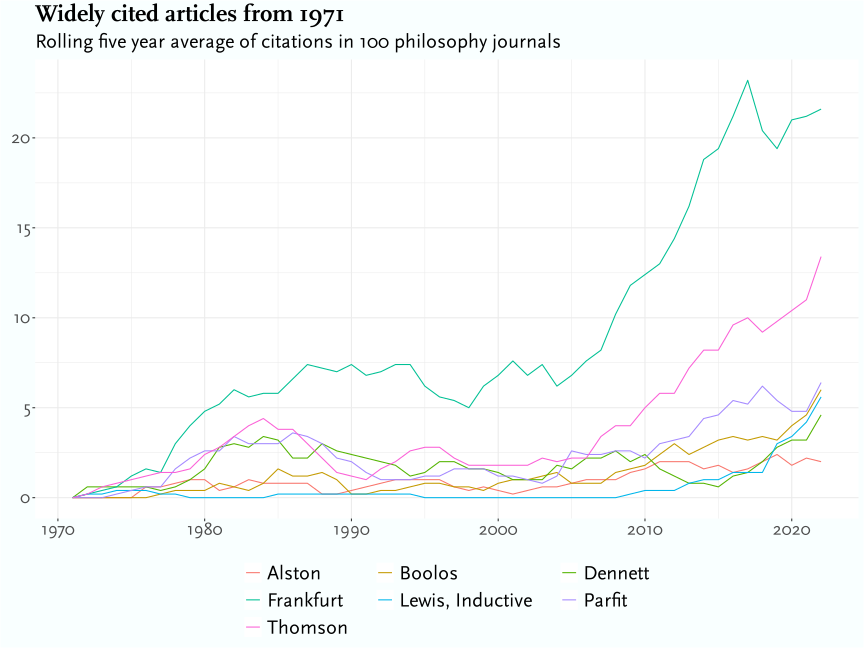
\includegraphics[keepaspectratio]{citations_files/figure-pdf/fig-citation-spaghetti-1971-1.pdf}}

}

\caption{\label{fig-citation-spaghetti-1971}Rolling five year average of
citation frequency for widely cited articles from 1971.}

\end{figure}%

\begin{figure}

\centering{

\pandocbounded{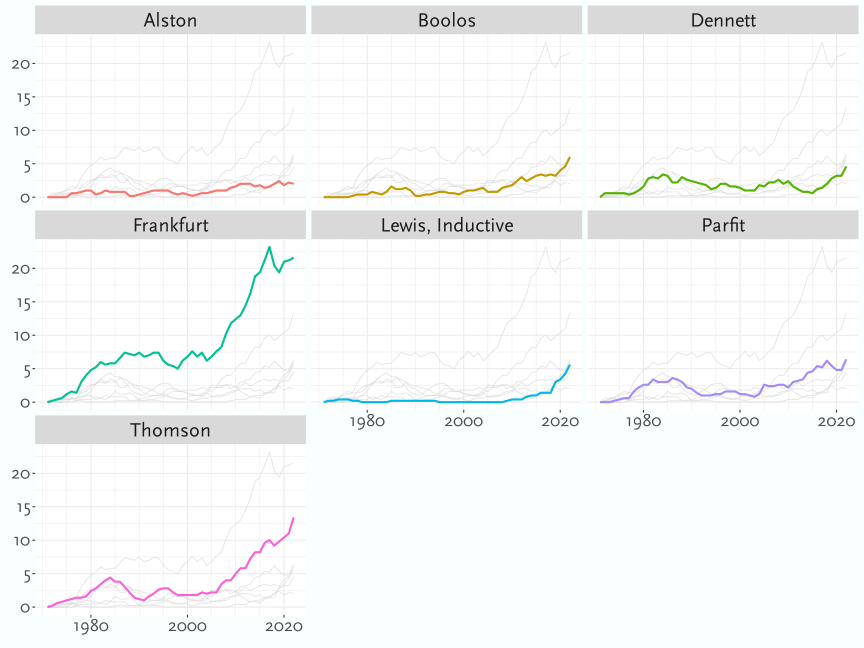
\includegraphics[keepaspectratio]{citations_files/figure-pdf/fig-citation-facet-1971-1.pdf}}

}

\caption{\label{fig-citation-facet-1971}Faceted version of
Figure~\ref{fig-citation-spaghetti-1971}.}

\end{figure}%

\newpage

\subsection{1972}\label{sec-s1972}

\subsubsection*{Widely Cited Articles}\label{widely-cited-articles-15}
\addcontentsline{toc}{subsubsection}{Widely Cited Articles}

\begin{enumerate}
\def\labelenumi{\arabic{enumi}.}
\tightlist
\item
  Peter Singer (\citeproc{ref-WOSA1972Z066400001}{1972}) ``Famine,
  Affluence, and Morality''
\item
  Hartry Field (\citeproc{ref-10.2307_2024879}{1972}) ``Tarski's Theory
  of Truth''
\item
  Philippa Foot (\citeproc{ref-WOSA1972N845400002}{1972}) ``Morality as
  a System of Hypothetical Imperatives''
\item
  Ned Block and Jerry A. Fodor (\citeproc{ref-WOSA1972YY85800002}{1972})
  ``What Psychological States Are Not''
\item
  Fred Dretske (\citeproc{ref-WOSA1972N864600001}{1972}) ``Contrastive
  Statements''
\item
  Richard Rorty (\citeproc{ref-10.2307_2025059}{1972}) ``The World Well
  Lost''
\item
  Gerald Dworkin (\citeproc{ref-WOSA1972N175300004}{1972})
  ``Paternalism''
\item
  Richard Routley and Robert K. Meyer
  (\citeproc{ref-WOSA1972Z110200006}{1972}) ``The Semantics of
  Entailment --- II''
\end{enumerate}

\subsubsection*{Citation Count}\label{sec-count-1972}
\addcontentsline{toc}{subsubsection}{Citation Count}


\begin{longtable}[]{@{}lrrr@{}}

\caption{\label{tbl-citation-count-1972}Citation count for widely cited
articles from 1972.}

\tabularnewline

\toprule\noalign{}
Article & All & Early & Late \\
\midrule\noalign{}
\endhead
\bottomrule\noalign{}
\endlastfoot
Singer (\citeproc{ref-WOSA1972Z066400001}{1972})
& 394 & 5 & 277 \\
Field (\citeproc{ref-10.2307_2024879}{1972})
& 136 & 29 & 22 \\
Foot (\citeproc{ref-WOSA1972N845400002}{1972})
& 131 & 15 & 77 \\
Block and Fodor (\citeproc{ref-WOSA1972YY85800002}{1972})
& 85 & 13 & 23 \\
Dretske (\citeproc{ref-WOSA1972N864600001}{1972})
& 65 & 11 & 18 \\
Rorty (\citeproc{ref-10.2307_2025059}{1972})
& 51 & 22 & 2 \\
G. Dworkin (\citeproc{ref-WOSA1972N175300004}{1972})
& 48 & 4 & 31 \\
Routley and Meyer (\citeproc{ref-WOSA1972Z110200006}{1972})
& 41 & 3 & 24 \\

\end{longtable}

\subsubsection*{Citation Rank}\label{sec-rank-1972}
\addcontentsline{toc}{subsubsection}{Citation Rank}


\begin{longtable}[]{@{}lrrr@{}}

\caption{\label{tbl-citation-rank-1972}Citation rank for widely cited
articles from 1972.}

\tabularnewline

\toprule\noalign{}
Article & Overall & Early & Late \\
\midrule\noalign{}
\endhead
\bottomrule\noalign{}
\endlastfoot
Singer (\citeproc{ref-WOSA1972Z066400001}{1972})
& 1 & 26 & 1 \\
Field (\citeproc{ref-10.2307_2024879}{1972})
& 2 & 1 & 6 \\
Foot (\citeproc{ref-WOSA1972N845400002}{1972})
& 3 & 4 & 2 \\
Block and Fodor (\citeproc{ref-WOSA1972YY85800002}{1972})
& 4 & 5 & 5 \\
Dretske (\citeproc{ref-WOSA1972N864600001}{1972})
& 5 & 8 & 10 \\
Rorty (\citeproc{ref-10.2307_2025059}{1972})
& 7 & 2 & 59 \\
G. Dworkin (\citeproc{ref-WOSA1972N175300004}{1972})
& 9 & 37 & 3 \\
Routley and Meyer (\citeproc{ref-WOSA1972Z110200006}{1972})
& 12 & 50 & 4 \\

\end{longtable}

\subsubsection*{Citation Trends}\label{sec-trends-1972}
\addcontentsline{toc}{subsubsection}{Citation Trends}

\begin{figure}

\centering{

\pandocbounded{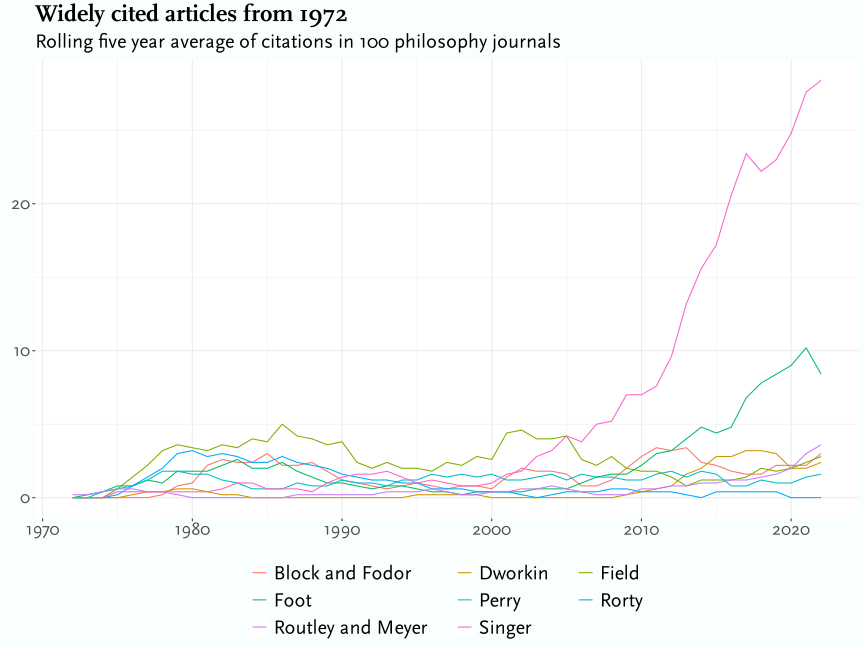
\includegraphics[keepaspectratio]{citations_files/figure-pdf/fig-citation-spaghetti-1972-1.pdf}}

}

\caption{\label{fig-citation-spaghetti-1972}Rolling five year average of
citation frequency for widely cited articles from 1972.}

\end{figure}%

\begin{figure}

\centering{

\pandocbounded{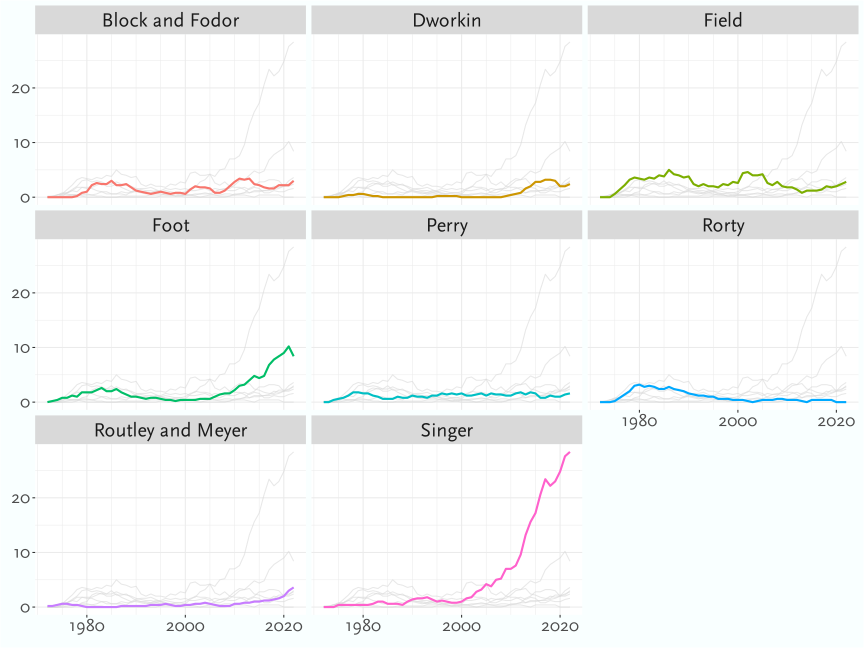
\includegraphics[keepaspectratio]{citations_files/figure-pdf/fig-citation-facet-1972-1.pdf}}

}

\caption{\label{fig-citation-facet-1972}Faceted version of
Figure~\ref{fig-citation-spaghetti-1972}.}

\end{figure}%

\newpage

\subsection{1973}\label{sec-s1973}

\subsubsection*{Widely Cited Articles}\label{widely-cited-articles-16}
\addcontentsline{toc}{subsubsection}{Widely Cited Articles}

\begin{enumerate}
\def\labelenumi{\arabic{enumi}.}
\tightlist
\item
  David Lewis (\citeproc{ref-10.2307_2025310}{1973}) ``Causation''
\item
  Paul Benacerraf (\citeproc{ref-10.2307_2025075}{1973}) ``Mathematical
  Truth''
\item
  Larry Wright (\citeproc{ref-WOSA1973P242100001}{1973}) ``Functions''
\item
  Hilary Putnam (\citeproc{ref-10.2307_2025079}{1973}) ``Meaning and
  Reference''
\item
  Hartry Field (\citeproc{ref-10.2307_2025110}{1973}) ``Theory Change
  and the Indeterminacy of Reference''
\item
  Jaegwon Kim (\citeproc{ref-10.2307_2025096}{1973}) ``Causation, Nomic
  Subsumption, and the Concept of Event''
\item
  Tyler Burge (\citeproc{ref-10.2307_2025107}{1973}) ``Reference and
  Proper Names''
\item
  Michael Walzer (\citeproc{ref-WOSA1973R219800003}{1973}) ``Political
  Action: The Problem of Dirty Hands''
\item
  Elie Zahar (\citeproc{ref-WOSA1973Q107900001}{1973}) ``Why Did
  Einsteins Programme Supersede Lorentzs (I)''
\end{enumerate}

\subsubsection*{Citation Count}\label{sec-count-1973}
\addcontentsline{toc}{subsubsection}{Citation Count}


\begin{longtable}[]{@{}lrrr@{}}

\caption{\label{tbl-citation-count-1973}Citation count for widely cited
articles from 1973.}

\tabularnewline

\toprule\noalign{}
Article & All & Early & Late \\
\midrule\noalign{}
\endhead
\bottomrule\noalign{}
\endlastfoot
Lewis (\citeproc{ref-10.2307_2025310}{1973})
& 461 & 44 & 234 \\
Benacerraf (\citeproc{ref-10.2307_2025075}{1973})
& 284 & 28 & 143 \\
L. Wright (\citeproc{ref-WOSA1973P242100001}{1973})
& 199 & 11 & 84 \\
Putnam (\citeproc{ref-10.2307_2025079}{1973})
& 177 & 39 & 86 \\
Field (\citeproc{ref-10.2307_2025110}{1973})
& 141 & 21 & 36 \\
Kim (\citeproc{ref-10.2307_2025096}{1973})
& 107 & 32 & 22 \\
Burge (\citeproc{ref-10.2307_2025107}{1973})
& 104 & 16 & 57 \\
Walzer (\citeproc{ref-WOSA1973R219800003}{1973})
& 64 & 5 & 39 \\
Zahar (\citeproc{ref-WOSA1973Q107900001}{1973})
& 54 & 19 & 12 \\

\end{longtable}

\subsubsection*{Citation Rank}\label{sec-rank-1973}
\addcontentsline{toc}{subsubsection}{Citation Rank}


\begin{longtable}[]{@{}lrrr@{}}

\caption{\label{tbl-citation-rank-1973}Citation rank for widely cited
articles from 1973.}

\tabularnewline

\toprule\noalign{}
Article & Overall & Early & Late \\
\midrule\noalign{}
\endhead
\bottomrule\noalign{}
\endlastfoot
Lewis (\citeproc{ref-10.2307_2025310}{1973})
& 1 & 1 & 1 \\
Benacerraf (\citeproc{ref-10.2307_2025075}{1973})
& 2 & 4 & 2 \\
L. Wright (\citeproc{ref-WOSA1973P242100001}{1973})
& 3 & 11 & 4 \\
Putnam (\citeproc{ref-10.2307_2025079}{1973})
& 4 & 2 & 3 \\
Field (\citeproc{ref-10.2307_2025110}{1973})
& 5 & 5 & 7 \\
Kim (\citeproc{ref-10.2307_2025096}{1973})
& 6 & 3 & 12 \\
Burge (\citeproc{ref-10.2307_2025107}{1973})
& 7 & 7 & 5 \\
Walzer (\citeproc{ref-WOSA1973R219800003}{1973})
& 10 & 32 & 6 \\
Zahar (\citeproc{ref-WOSA1973Q107900001}{1973})
& 14 & 6 & 19 \\

\end{longtable}

\subsubsection*{Citation Trends}\label{sec-trends-1973}
\addcontentsline{toc}{subsubsection}{Citation Trends}

\begin{figure}

\centering{

\pandocbounded{\includegraphics[keepaspectratio]{citations_files/figure-pdf/fig-citation-spaghetti-1973-1.pdf}}

}

\caption{\label{fig-citation-spaghetti-1973}Rolling five year average of
citation frequency for widely cited articles from 1973.}

\end{figure}%

\begin{figure}

\centering{

\pandocbounded{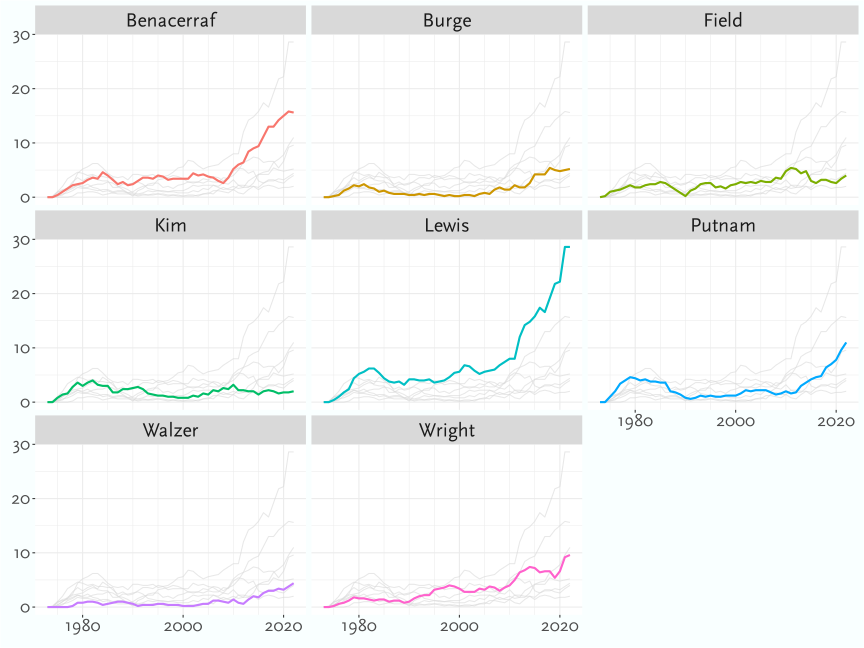
\includegraphics[keepaspectratio]{citations_files/figure-pdf/fig-citation-facet-1973-1.pdf}}

}

\caption{\label{fig-citation-facet-1973}Faceted version of
Figure~\ref{fig-citation-spaghetti-1973}.}

\end{figure}%

\newpage

\subsection{1974}\label{sec-s1974}

\subsubsection*{Widely Cited Articles}\label{widely-cited-articles-17}
\addcontentsline{toc}{subsubsection}{Widely Cited Articles}

\begin{enumerate}
\def\labelenumi{\arabic{enumi}.}
\tightlist
\item
  Thomas Nagel (\citeproc{ref-WOSA1974U469700001}{1974}) ``What is It
  Like To Be a Bat''
\item
  Michael Friedman (\citeproc{ref-10.2307_2024924}{1974}) ``Explanation
  and Scientific Understanding''
\item
  Isaac Levi (\citeproc{ref-10.2307_2025161}{1974}) ``On Indeterminate
  Probabilities''
\item
  Keith S. Donnellan (\citeproc{ref-WOSA1974R925600001}{1974})
  ``Speaking of Nothing''
\item
  Charles Parsons (\citeproc{ref-WOSA1974U793100003}{1974}) ``The Liar
  Paradox''
\item
  Peter Singer (\citeproc{ref-WOSA1974U371600008}{1974}) ``Sidgwick and
  Reflective Equilibrium''
\item
  Michael Devitt (\citeproc{ref-10.2307_2025347}{1974}) ``Singular
  Terms''
\end{enumerate}

\subsubsection*{Citation Count}\label{sec-count-1974}
\addcontentsline{toc}{subsubsection}{Citation Count}


\begin{longtable}[]{@{}lrrr@{}}

\caption{\label{tbl-citation-count-1974}Citation count for widely cited
articles from 1974.}

\tabularnewline

\toprule\noalign{}
Article & All & Early & Late \\
\midrule\noalign{}
\endhead
\bottomrule\noalign{}
\endlastfoot
Nagel (\citeproc{ref-WOSA1974U469700001}{1974})
& 644 & 16 & 312 \\
M. Friedman (\citeproc{ref-10.2307_2024924}{1974})
& 245 & 12 & 119 \\
Levi (\citeproc{ref-10.2307_2025161}{1974})
& 138 & 15 & 69 \\
Donnellan (\citeproc{ref-WOSA1974R925600001}{1974})
& 87 & 19 & 30 \\
Parsons (\citeproc{ref-WOSA1974U793100003}{1974})
& 73 & 10 & 33 \\
Singer (\citeproc{ref-WOSA1974U371600008}{1974})
& 66 & 9 & 30 \\
Devitt (\citeproc{ref-10.2307_2025347}{1974})
& 50 & 25 & 13 \\

\end{longtable}

\subsubsection*{Citation Rank}\label{sec-rank-1974}
\addcontentsline{toc}{subsubsection}{Citation Rank}


\begin{longtable}[]{@{}lrrr@{}}

\caption{\label{tbl-citation-rank-1974}Citation rank for widely cited
articles from 1974.}

\tabularnewline

\toprule\noalign{}
Article & Overall & Early & Late \\
\midrule\noalign{}
\endhead
\bottomrule\noalign{}
\endlastfoot
Nagel (\citeproc{ref-WOSA1974U469700001}{1974})
& 1 & 4 & 1 \\
M. Friedman (\citeproc{ref-10.2307_2024924}{1974})
& 2 & 8 & 2 \\
Levi (\citeproc{ref-10.2307_2025161}{1974})
& 3 & 5 & 3 \\
Donnellan (\citeproc{ref-WOSA1974R925600001}{1974})
& 4 & 2 & 5 \\
Parsons (\citeproc{ref-WOSA1974U793100003}{1974})
& 5 & 12 & 4 \\
Singer (\citeproc{ref-WOSA1974U371600008}{1974})
& 6 & 17 & 5 \\
Devitt (\citeproc{ref-10.2307_2025347}{1974})
& 8 & 1 & 13 \\

\end{longtable}

\subsubsection*{Citation Trends}\label{sec-trends-1974}
\addcontentsline{toc}{subsubsection}{Citation Trends}

\begin{figure}

\centering{

\pandocbounded{\includegraphics[keepaspectratio]{citations_files/figure-pdf/fig-citation-spaghetti-1974-1.pdf}}

}

\caption{\label{fig-citation-spaghetti-1974}Rolling five year average of
citation frequency for widely cited articles from 1974.}

\end{figure}%

\begin{figure}

\centering{

\pandocbounded{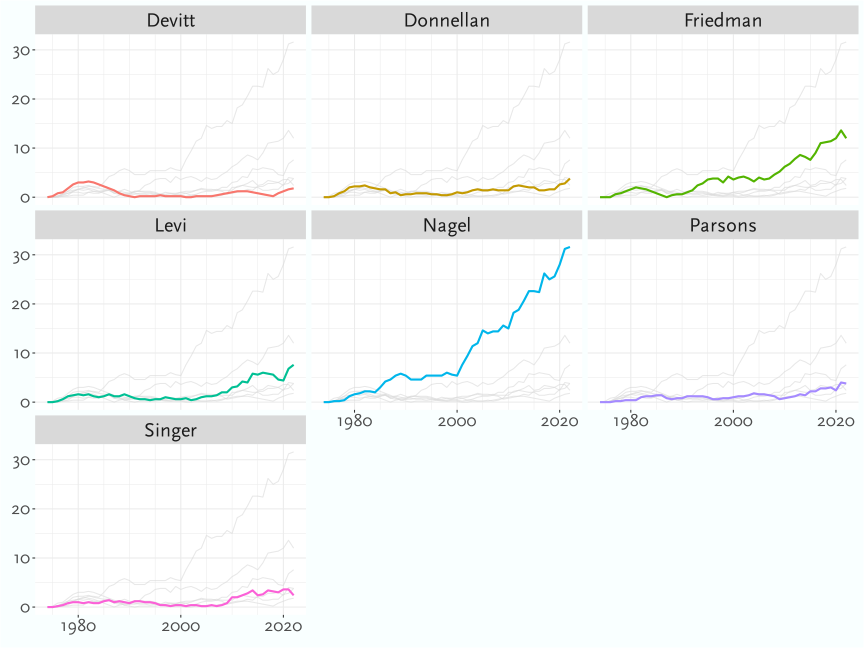
\includegraphics[keepaspectratio]{citations_files/figure-pdf/fig-citation-facet-1974-1.pdf}}

}

\caption{\label{fig-citation-facet-1974}Faceted version of
Figure~\ref{fig-citation-spaghetti-1974}.}

\end{figure}%

\newpage

\subsection{1975}\label{sec-s1975}

\subsubsection*{Widely Cited Articles}\label{widely-cited-articles-18}
\addcontentsline{toc}{subsubsection}{Widely Cited Articles}

\begin{enumerate}
\def\labelenumi{\arabic{enumi}.}
\tightlist
\item
  Saul Kripke (\citeproc{ref-WOSA1975BF60000005}{1975}) ``Outline of a
  Theory of Truth''
\item
  Robert Cummins (\citeproc{ref-WOSA1975BF60100001}{1975}) ``Functional
  Analysis''
\item
  Gary Watson (\citeproc{ref-WOSA1975W282300001}{1975}) ``Free Agency''
\item
  Allan Gibbard (\citeproc{ref-WOSA1975AU08300005}{1975}) ``Contingent
  Identity''
\item
  Robert C. Stalnaker (\citeproc{ref-WOSA1975LD17700007}{1975})
  ``Indicative Conditionals''
\item
  Gilbert Harman (\citeproc{ref-WOSA1975V416000001}{1975}) ``Moral
  Relativism Defended''
\item
  Dorothy L. Grover, Joseph L. Camp Jr., and Nuel D. Belnap Jr.
  (\citeproc{ref-WOSA1975BC66900001}{1975}) ``A Pro-Sentential Theory of
  Truth''
\item
  Geoffrey Paul Hellman and Frank Wilson Thompson
  (\citeproc{ref-WOSA1975AT43400003}{1975}) ``Physicalism: Ontology,
  Determination, and Reduction''
\item
  David Kaplan (\citeproc{ref-WOSA1975BF60000006}{1975}) ``Sets,
  Concepts and Extensions: How To Russell a Frege-Church''
\end{enumerate}

\subsubsection*{Citation Count}\label{sec-count-1975}
\addcontentsline{toc}{subsubsection}{Citation Count}


\begin{longtable}[]{@{}lrrr@{}}

\caption{\label{tbl-citation-count-1975}Citation count for widely cited
articles from 1975.}

\tabularnewline

\toprule\noalign{}
Article & All & Early & Late \\
\midrule\noalign{}
\endhead
\bottomrule\noalign{}
\endlastfoot
Kripke (\citeproc{ref-WOSA1975BF60000005}{1975})
& 455 & 48 & 220 \\
Cummins (\citeproc{ref-WOSA1975BF60100001}{1975})
& 347 & 17 & 152 \\
Watson (\citeproc{ref-WOSA1975W282300001}{1975})
& 230 & 20 & 111 \\
Gibbard (\citeproc{ref-WOSA1975AU08300005}{1975})
& 142 & 5 & 62 \\
Stalnaker (\citeproc{ref-WOSA1975LD17700007}{1975})
& 135 & 3 & 98 \\
Harman (\citeproc{ref-WOSA1975V416000001}{1975})
& 109 & 14 & 47 \\
Grover, Jr., and Jr. (\citeproc{ref-WOSA1975BC66900001}{1975})
& 86 & 14 & 22 \\
Hellman and Thompson (\citeproc{ref-WOSA1975AT43400003}{1975})
& 73 & 19 & 6 \\
D. Kaplan (\citeproc{ref-WOSA1975BF60000006}{1975})
& 66 & 15 & 18 \\

\end{longtable}

\subsubsection*{Citation Rank}\label{sec-rank-1975}
\addcontentsline{toc}{subsubsection}{Citation Rank}


\begin{longtable}[]{@{}lrrr@{}}

\caption{\label{tbl-citation-rank-1975}Citation rank for widely cited
articles from 1975.}

\tabularnewline

\toprule\noalign{}
Article & Overall & Early & Late \\
\midrule\noalign{}
\endhead
\bottomrule\noalign{}
\endlastfoot
Kripke (\citeproc{ref-WOSA1975BF60000005}{1975})
& 1 & 1 & 1 \\
Cummins (\citeproc{ref-WOSA1975BF60100001}{1975})
& 2 & 4 & 2 \\
Watson (\citeproc{ref-WOSA1975W282300001}{1975})
& 3 & 2 & 3 \\
Gibbard (\citeproc{ref-WOSA1975AU08300005}{1975})
& 4 & 43 & 5 \\
Stalnaker (\citeproc{ref-WOSA1975LD17700007}{1975})
& 5 & 79 & 4 \\
Harman (\citeproc{ref-WOSA1975V416000001}{1975})
& 6 & 6 & 6 \\
Grover, Jr., and Jr. (\citeproc{ref-WOSA1975BC66900001}{1975})
& 7 & 6 & 13 \\
Hellman and Thompson (\citeproc{ref-WOSA1975AT43400003}{1975})
& 8 & 3 & 37 \\
D. Kaplan (\citeproc{ref-WOSA1975BF60000006}{1975})
& 9 & 5 & 17 \\

\end{longtable}

\subsubsection*{Citation Trends}\label{sec-trends-1975}
\addcontentsline{toc}{subsubsection}{Citation Trends}

\begin{figure}

\centering{

\pandocbounded{\includegraphics[keepaspectratio]{citations_files/figure-pdf/fig-citation-spaghetti-1975-1.pdf}}

}

\caption{\label{fig-citation-spaghetti-1975}Rolling five year average of
citation frequency for widely cited articles from 1975.}

\end{figure}%

\begin{figure}

\centering{

\pandocbounded{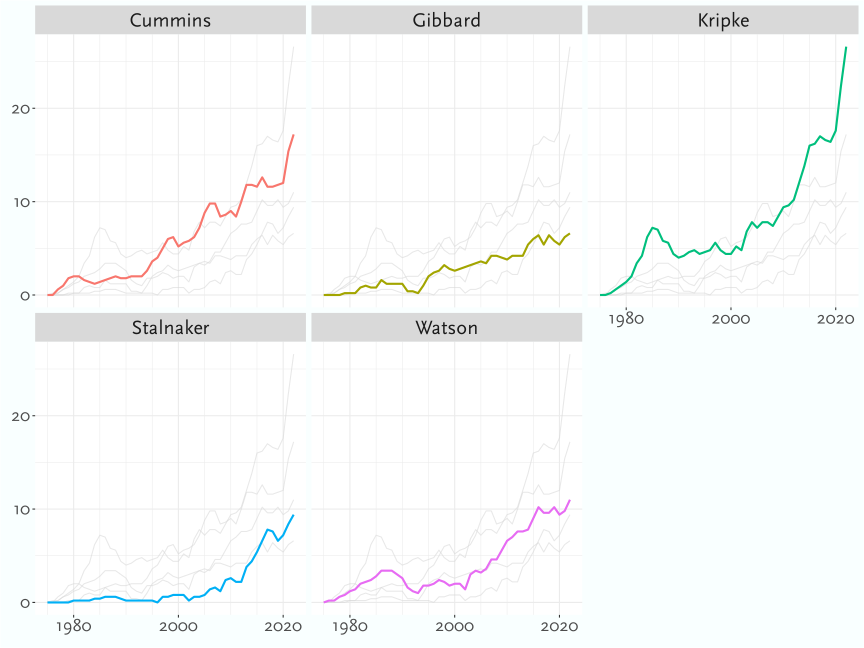
\includegraphics[keepaspectratio]{citations_files/figure-pdf/fig-citation-facet-1975-1.pdf}}

}

\caption{\label{fig-citation-facet-1975}Faceted version of
Figure~\ref{fig-citation-spaghetti-1975}.}

\end{figure}%

\newpage

\subsection{1976}\label{sec-s1976}

\subsubsection*{Widely Cited Articles}\label{widely-cited-articles-19}
\addcontentsline{toc}{subsubsection}{Widely Cited Articles}

\begin{enumerate}
\def\labelenumi{\arabic{enumi}.}
\tightlist
\item
  Alvin I. Goldman (\citeproc{ref-WOSA1976CP00100001}{1976})
  ``Discrimination and Perceptual Knowledge''
\item
  David Lewis (\citeproc{ref-WOSA1976BZ95100001}{1976b}) ``Probabilities
  of Conditionals and Conditional Probabilities''
\item
  David Lewis (\citeproc{ref-WOSA1976BF01500006}{1976a}) ``Paradoxes of
  Time Travel''
\item
  Michael Stocker (\citeproc{ref-WOSA1976CB49000002}{1976}) ``The
  Schizophrenia of Modern Ethical Theories''
\item
  Gilbert Harman (\citeproc{ref-WOSA1976BK58800002}{1976}) ``Practical
  Reasoning''
\item
  Robert C. Stalnaker (\citeproc{ref-WOSA1976GM48400006}{1976})
  ``Possible Worlds''
\item
  J. Michael Dunn (\citeproc{ref-WOSA1976EK38200001}{1976}) ``Intuitive
  Semantics for First-Degree Entailments and Coupled Trees''
\item
  Robert Merrihew Adams (\citeproc{ref-WOSA1976CB49000003}{1976})
  ``Motive Utilitarianism''
\item
  Brian Loar (\citeproc{ref-WOSA1976EK39100001}{1976}) ``The Semantics
  of Singular Terms''
\end{enumerate}

\subsubsection*{Citation Count}\label{sec-count-1976}
\addcontentsline{toc}{subsubsection}{Citation Count}


\begin{longtable}[]{@{}lrrr@{}}

\caption{\label{tbl-citation-count-1976}Citation count for widely cited
articles from 1976.}

\tabularnewline

\toprule\noalign{}
Article & All & Early & Late \\
\midrule\noalign{}
\endhead
\bottomrule\noalign{}
\endlastfoot
Goldman (\citeproc{ref-WOSA1976CP00100001}{1976})
& 406 & 48 & 199 \\
Lewis (\citeproc{ref-WOSA1976BZ95100001}{1976b})
& 260 & 29 & 125 \\
Lewis (\citeproc{ref-WOSA1976BF01500006}{1976a})
& 173 & 12 & 110 \\
Stocker (\citeproc{ref-WOSA1976CB49000002}{1976})
& 150 & 10 & 64 \\
Harman (\citeproc{ref-WOSA1976BK58800002}{1976})
& 137 & 14 & 70 \\
Stalnaker (\citeproc{ref-WOSA1976GM48400006}{1976})
& 99 & 10 & 57 \\
Dunn (\citeproc{ref-WOSA1976EK38200001}{1976})
& 91 & 7 & 62 \\
R. M. Adams (\citeproc{ref-WOSA1976CB49000003}{1976})
& 55 & 11 & 18 \\
Loar (\citeproc{ref-WOSA1976EK39100001}{1976})
& 47 & 11 & 20 \\

\end{longtable}

\subsubsection*{Citation Rank}\label{sec-rank-1976}
\addcontentsline{toc}{subsubsection}{Citation Rank}


\begin{longtable}[]{@{}lrrr@{}}

\caption{\label{tbl-citation-rank-1976}Citation rank for widely cited
articles from 1976.}

\tabularnewline

\toprule\noalign{}
Article & Overall & Early & Late \\
\midrule\noalign{}
\endhead
\bottomrule\noalign{}
\endlastfoot
Goldman (\citeproc{ref-WOSA1976CP00100001}{1976})
& 1 & 1 & 1 \\
Lewis (\citeproc{ref-WOSA1976BZ95100001}{1976b})
& 2 & 2 & 2 \\
Lewis (\citeproc{ref-WOSA1976BF01500006}{1976a})
& 3 & 5 & 3 \\
Stocker (\citeproc{ref-WOSA1976CB49000002}{1976})
& 4 & 10 & 5 \\
Harman (\citeproc{ref-WOSA1976BK58800002}{1976})
& 5 & 4 & 4 \\
Stalnaker (\citeproc{ref-WOSA1976GM48400006}{1976})
& 6 & 10 & 7 \\
Dunn (\citeproc{ref-WOSA1976EK38200001}{1976})
& 8 & 22 & 6 \\
R. M. Adams (\citeproc{ref-WOSA1976CB49000003}{1976})
& 10 & 6 & 15 \\
Loar (\citeproc{ref-WOSA1976EK39100001}{1976})
& 11 & 6 & 11 \\

\end{longtable}

\subsubsection*{Citation Trends}\label{sec-trends-1976}
\addcontentsline{toc}{subsubsection}{Citation Trends}

\begin{figure}

\centering{

\pandocbounded{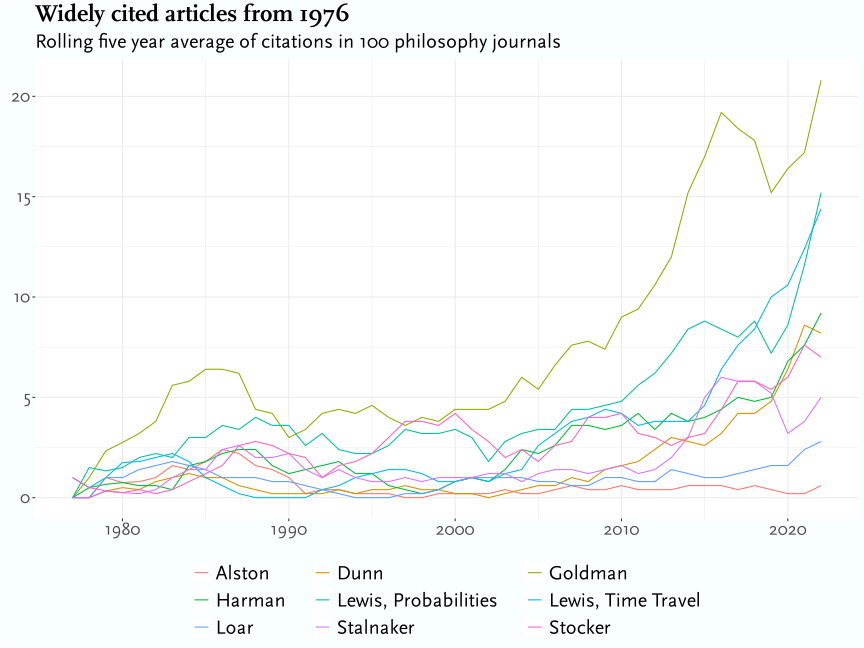
\includegraphics[keepaspectratio]{citations_files/figure-pdf/fig-citation-spaghetti-1976-1.pdf}}

}

\caption{\label{fig-citation-spaghetti-1976}Rolling five year average of
citation frequency for widely cited articles from 1976.}

\end{figure}%

\begin{figure}

\centering{

\pandocbounded{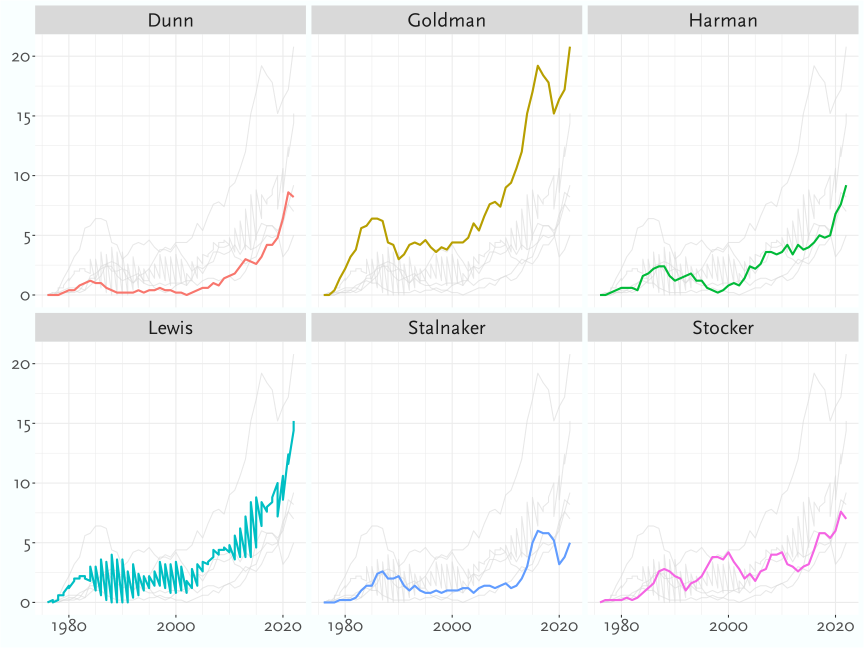
\includegraphics[keepaspectratio]{citations_files/figure-pdf/fig-citation-facet-1976-1.pdf}}

}

\caption{\label{fig-citation-facet-1976}Faceted version of
Figure~\ref{fig-citation-spaghetti-1976}.}

\end{figure}%

\newpage

\subsection{1977}\label{sec-s1977}

\subsubsection*{Widely Cited Articles}\label{widely-cited-articles-20}
\addcontentsline{toc}{subsubsection}{Widely Cited Articles}

\begin{enumerate}
\def\labelenumi{\arabic{enumi}.}
\tightlist
\item
  John Perry (\citeproc{ref-WOSA1977EA01800002}{1977}) ``Frege on
  Demonstratives''
\item
  Stephen L. Darwall (\citeproc{ref-WOSA1977EA35800003}{1977}) ``Two
  Kinds of Respect''
\item
  Fred Dretske (\citeproc{ref-WOSA1977DN52600007}{1977}) ``Laws of
  Nature''
\item
  Michael Tooley (\citeproc{ref-WOSA1977EQ83600001}{1977}) ``Nature of
  Laws''
\item
  John M. Taurek (\citeproc{ref-WOSA1977DX39800001}{1977}) ``Should the
  Numbers Count?''
\item
  Tyler Burge (\citeproc{ref-WOSA1977DH28800002}{1977}) ``Belief De Re''
\item
  Christopher Boorse (\citeproc{ref-WOSA1977ES93500003}{1977}) ``Health
  as a Theoretical Concept''
\item
  Hartry Field (\citeproc{ref-WOSA1977DN99500001}{1977}) ``Logic,
  Meaning, and Conceptual Role''
\item
  Hector-Neri Castañeda (\citeproc{ref-WOSA1977DV15800002}{1977})
  ``Perception, Belief, and Structure of Physical Objects and
  Consciousness''
\end{enumerate}

\subsubsection*{Citation Count}\label{sec-count-1977}
\addcontentsline{toc}{subsubsection}{Citation Count}


\begin{longtable}[]{@{}lrrr@{}}

\caption{\label{tbl-citation-count-1977}Citation count for widely cited
articles from 1977.}

\tabularnewline

\toprule\noalign{}
Article & All & Early & Late \\
\midrule\noalign{}
\endhead
\bottomrule\noalign{}
\endlastfoot
Perry (\citeproc{ref-WOSA1977EA01800002}{1977})
& 204 & 32 & 83 \\
Darwall (\citeproc{ref-WOSA1977EA35800003}{1977})
& 203 & 3 & 145 \\
Dretske (\citeproc{ref-WOSA1977DN52600007}{1977})
& 196 & 18 & 87 \\
Tooley (\citeproc{ref-WOSA1977EQ83600001}{1977})
& 182 & 15 & 86 \\
Taurek (\citeproc{ref-WOSA1977DX39800001}{1977})
& 152 & 12 & 82 \\
Burge (\citeproc{ref-WOSA1977DH28800002}{1977})
& 115 & 33 & 30 \\
Boorse (\citeproc{ref-WOSA1977ES93500003}{1977})
& 114 & 3 & 77 \\
Field (\citeproc{ref-WOSA1977DN99500001}{1977})
& 84 & 21 & 22 \\
Castañeda (\citeproc{ref-WOSA1977DV15800002}{1977})
& 37 & 27 & 1 \\

\end{longtable}

\subsubsection*{Citation Rank}\label{sec-rank-1977}
\addcontentsline{toc}{subsubsection}{Citation Rank}


\begin{longtable}[]{@{}lrrr@{}}

\caption{\label{tbl-citation-rank-1977}Citation rank for widely cited
articles from 1977.}

\tabularnewline

\toprule\noalign{}
Article & Overall & Early & Late \\
\midrule\noalign{}
\endhead
\bottomrule\noalign{}
\endlastfoot
Perry (\citeproc{ref-WOSA1977EA01800002}{1977})
& 1 & 2 & 4 \\
Darwall (\citeproc{ref-WOSA1977EA35800003}{1977})
& 2 & 87 & 1 \\
Dretske (\citeproc{ref-WOSA1977DN52600007}{1977})
& 3 & 5 & 2 \\
Tooley (\citeproc{ref-WOSA1977EQ83600001}{1977})
& 4 & 6 & 3 \\
Taurek (\citeproc{ref-WOSA1977DX39800001}{1977})
& 5 & 10 & 5 \\
Burge (\citeproc{ref-WOSA1977DH28800002}{1977})
& 6 & 1 & 10 \\
Boorse (\citeproc{ref-WOSA1977ES93500003}{1977})
& 7 & 87 & 6 \\
Field (\citeproc{ref-WOSA1977DN99500001}{1977})
& 9 & 4 & 15 \\
Castañeda (\citeproc{ref-WOSA1977DV15800002}{1977})
& 19 & 3 & 164 \\

\end{longtable}

\subsubsection*{Citation Trends}\label{sec-trends-1977}
\addcontentsline{toc}{subsubsection}{Citation Trends}

\begin{figure}

\centering{

\pandocbounded{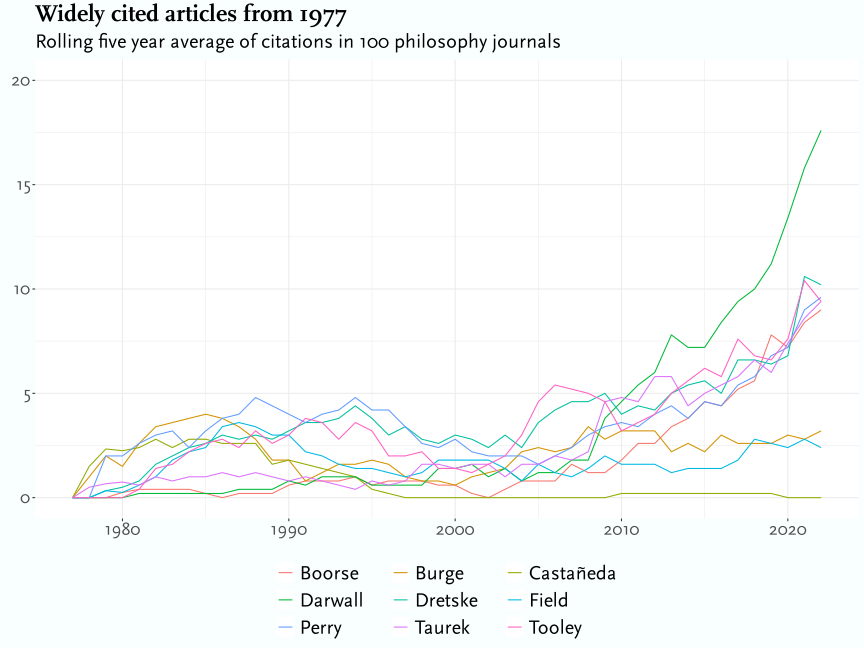
\includegraphics[keepaspectratio]{citations_files/figure-pdf/fig-citation-spaghetti-1977-1.pdf}}

}

\caption{\label{fig-citation-spaghetti-1977}Rolling five year average of
citation frequency for widely cited articles from 1977.}

\end{figure}%

\begin{figure}

\centering{

\pandocbounded{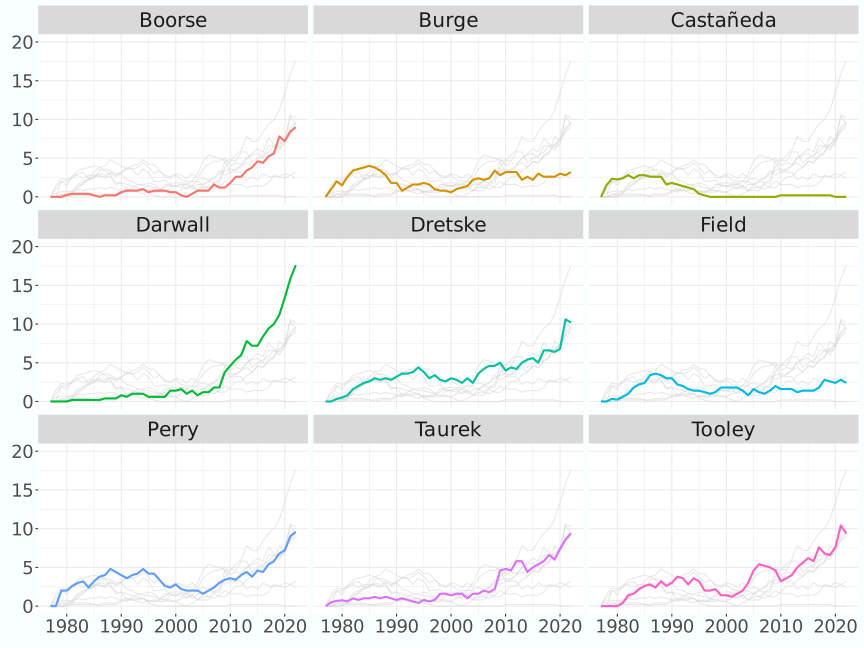
\includegraphics[keepaspectratio]{citations_files/figure-pdf/fig-citation-facet-1977-1.pdf}}

}

\caption{\label{fig-citation-facet-1977}Faceted version of
Figure~\ref{fig-citation-spaghetti-1977}.}

\end{figure}%

\newpage

\subsection{1978}\label{sec-s1978}

\subsubsection*{Widely Cited Articles}\label{widely-cited-articles-21}
\addcontentsline{toc}{subsubsection}{Widely Cited Articles}

\begin{enumerate}
\def\labelenumi{\arabic{enumi}.}
\tightlist
\item
  David Lewis (\citeproc{ref-WOSA1978ER30500004}{1978}) ``Truth in
  Fiction''
\item
  David L. Hull (\citeproc{ref-WOSA1978FR68900001}{1978}) ``A Matter of
  Individuality''
\item
  Kendall L. Walton (\citeproc{ref-WOSA1978EK23200001}{1978}) ``Fearing
  Fictions''
\item
  Stephen P. Stich (\citeproc{ref-WOSA1978GH93900001}{1978}) ``Beliefs
  and Subdoxastic States''
\item
  Harry G. Frankfurt (\citeproc{ref-WOSA1978EL93700010}{1978}) ``The
  Problem of Action''
\item
  Paul R. Thagard (\citeproc{ref-WOSA1978EP78600002}{1978}) ``The Best
  Explanation: Criteria for Theory Choice''
\item
  Jaegwon Kim (\citeproc{ref-WOSA1978EL93700009}{1978}) ``Supervenience
  and Nomological Incommensurables''
\item
  L BonJour (\citeproc{ref-WOSA1978ER30500001}{1978}) ``Can Empirical
  Knowledge Have a Foundation?''
\item
  Gregory S. Kavka (\citeproc{ref-WOSA1978FB55500001}{1978}) ``Some
  Paradoxes of Deterrence''
\end{enumerate}

\subsubsection*{Citation Count}\label{sec-count-1978}
\addcontentsline{toc}{subsubsection}{Citation Count}


\begin{longtable}[]{@{}lrrr@{}}

\caption{\label{tbl-citation-count-1978}Citation count for widely cited
articles from 1978.}

\tabularnewline

\toprule\noalign{}
Article & All & Early & Late \\
\midrule\noalign{}
\endhead
\bottomrule\noalign{}
\endlastfoot
Lewis (\citeproc{ref-WOSA1978ER30500004}{1978})
& 177 & 18 & 110 \\
Hull (\citeproc{ref-WOSA1978FR68900001}{1978})
& 146 & 16 & 52 \\
Walton (\citeproc{ref-WOSA1978EK23200001}{1978})
& 99 & 22 & 45 \\
Stich (\citeproc{ref-WOSA1978GH93900001}{1978})
& 94 & 5 & 41 \\
Frankfurt (\citeproc{ref-WOSA1978EL93700010}{1978})
& 86 & 7 & 62 \\
Thagard (\citeproc{ref-WOSA1978EP78600002}{1978})
& 86 & 9 & 50 \\
Kim (\citeproc{ref-WOSA1978EL93700009}{1978})
& 76 & 33 & 2 \\
BonJour (\citeproc{ref-WOSA1978ER30500001}{1978})
& 55 & 18 & 16 \\
Kavka (\citeproc{ref-WOSA1978FB55500001}{1978})
& 45 & 19 & 4 \\

\end{longtable}

\subsubsection*{Citation Rank}\label{sec-rank-1978}
\addcontentsline{toc}{subsubsection}{Citation Rank}


\begin{longtable}[]{@{}lrrr@{}}

\caption{\label{tbl-citation-rank-1978}Citation rank for widely cited
articles from 1978.}

\tabularnewline

\toprule\noalign{}
Article & Overall & Early & Late \\
\midrule\noalign{}
\endhead
\bottomrule\noalign{}
\endlastfoot
Lewis (\citeproc{ref-WOSA1978ER30500004}{1978})
& 1 & 4 & 1 \\
Hull (\citeproc{ref-WOSA1978FR68900001}{1978})
& 2 & 7 & 3 \\
Walton (\citeproc{ref-WOSA1978EK23200001}{1978})
& 3 & 2 & 6 \\
Stich (\citeproc{ref-WOSA1978GH93900001}{1978})
& 4 & 48 & 7 \\
Frankfurt (\citeproc{ref-WOSA1978EL93700010}{1978})
& 5 & 28 & 2 \\
Thagard (\citeproc{ref-WOSA1978EP78600002}{1978})
& 5 & 21 & 4 \\
Kim (\citeproc{ref-WOSA1978EL93700009}{1978})
& 7 & 1 & 95 \\
BonJour (\citeproc{ref-WOSA1978ER30500001}{1978})
& 12 & 4 & 15 \\
Kavka (\citeproc{ref-WOSA1978FB55500001}{1978})
& 18 & 3 & 59 \\

\end{longtable}

\subsubsection*{Citation Trends}\label{sec-trends-1978}
\addcontentsline{toc}{subsubsection}{Citation Trends}

\begin{figure}

\centering{

\pandocbounded{\includegraphics[keepaspectratio]{citations_files/figure-pdf/fig-citation-spaghetti-1978-1.pdf}}

}

\caption{\label{fig-citation-spaghetti-1978}Rolling five year average of
citation frequency for widely cited articles from 1978.}

\end{figure}%

\begin{figure}

\centering{

\pandocbounded{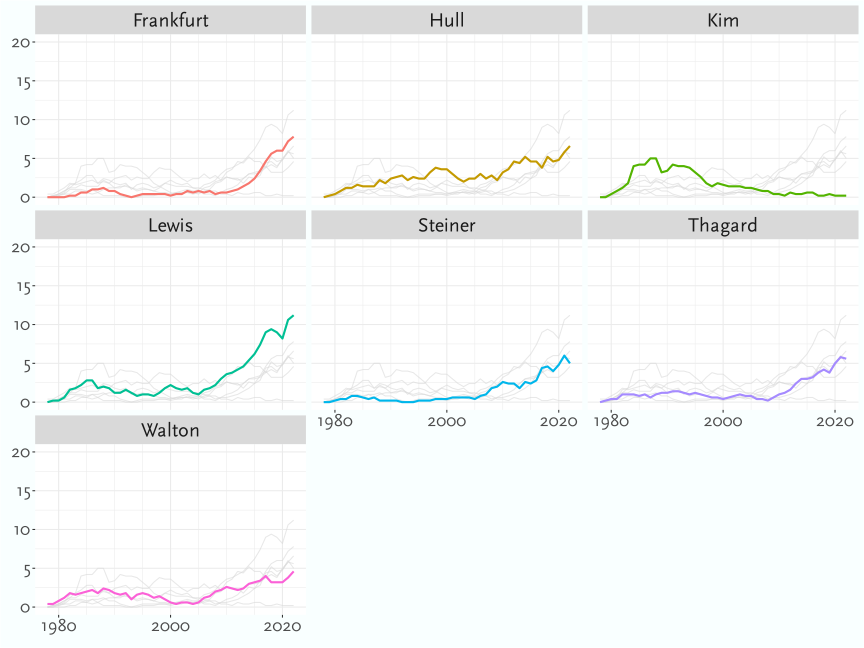
\includegraphics[keepaspectratio]{citations_files/figure-pdf/fig-citation-facet-1978-1.pdf}}

}

\caption{\label{fig-citation-facet-1978}Faceted version of
Figure~\ref{fig-citation-spaghetti-1978}.}

\end{figure}%

\newpage

\subsection{1979}\label{sec-s1979}

\subsubsection*{Widely Cited Articles}\label{widely-cited-articles-22}
\addcontentsline{toc}{subsubsection}{Widely Cited Articles}

\begin{enumerate}
\def\labelenumi{\arabic{enumi}.}
\tightlist
\item
  John Perry (\citeproc{ref-WOSA1979HE39600001}{1979}) ``The Problem of
  the Essential Indexical''
\item
  David Lewis (\citeproc{ref-WOSA1979JC64200001}{1979a}) ``Attitudes De
  Dicto and De Se''
\item
  David Lewis (\citeproc{ref-WOSA1979HJ57600007}{1979c}) ``Scorekeeping
  in a Language Game''
\item
  David Lewis (\citeproc{ref-WOSA1979JB14500003}{1979b})
  ``Counterfactual Dependence and Time's Arrow''
\item
  John McDowell (\citeproc{ref-WOSA1979JT33600005}{1979}) ``Virtue and
  Reason''
\item
  Graham Priest (\citeproc{ref-WOSA1979GW33200004}{1979}) ``The Logic of
  Paradox''
\item
  Norman Daniels (\citeproc{ref-WOSA1979GW47300003}{1979}) ``Wide
  Reflective Equilibrium and Theory Acceptance in Ethics''
\item
  Nancy Cartwright (\citeproc{ref-WOSA1979JB14500001}{1979}) ``Causal
  Laws and Effective Strategies''
\item
  Daniel Lascar and Bruno Poizat
  (\citeproc{ref-WOSA1979HL22300006}{1979}) ``Introduction To Forking''
\end{enumerate}

\subsubsection*{Citation Count}\label{sec-count-1979}
\addcontentsline{toc}{subsubsection}{Citation Count}


\begin{longtable}[]{@{}lrrr@{}}

\caption{\label{tbl-citation-count-1979}Citation count for widely cited
articles from 1979.}

\tabularnewline

\toprule\noalign{}
Article & All & Early & Late \\
\midrule\noalign{}
\endhead
\bottomrule\noalign{}
\endlastfoot
Perry (\citeproc{ref-WOSA1979HE39600001}{1979})
& 420 & 61 & 188 \\
Lewis (\citeproc{ref-WOSA1979JC64200001}{1979a})
& 411 & 33 & 247 \\
Lewis (\citeproc{ref-WOSA1979HJ57600007}{1979c})
& 402 & 17 & 232 \\
Lewis (\citeproc{ref-WOSA1979JB14500003}{1979b})
& 381 & 38 & 200 \\
McDowell (\citeproc{ref-WOSA1979JT33600005}{1979})
& 229 & 13 & 95 \\
Priest (\citeproc{ref-WOSA1979GW33200004}{1979})
& 213 & 16 & 146 \\
Daniels (\citeproc{ref-WOSA1979GW47300003}{1979})
& 149 & 41 & 54 \\
Cartwright (\citeproc{ref-WOSA1979JB14500001}{1979})
& 130 & 29 & 50 \\
Lascar and Poizat (\citeproc{ref-WOSA1979HL22300006}{1979})
& 34 & 23 & 1 \\

\end{longtable}

\subsubsection*{Citation Rank}\label{sec-rank-1979}
\addcontentsline{toc}{subsubsection}{Citation Rank}


\begin{longtable}[]{@{}lrrr@{}}

\caption{\label{tbl-citation-rank-1979}Citation rank for widely cited
articles from 1979.}

\tabularnewline

\toprule\noalign{}
Article & Overall & Early & Late \\
\midrule\noalign{}
\endhead
\bottomrule\noalign{}
\endlastfoot
Perry (\citeproc{ref-WOSA1979HE39600001}{1979})
& 1 & 1 & 4 \\
Lewis (\citeproc{ref-WOSA1979JC64200001}{1979a})
& 2 & 4 & 1 \\
Lewis (\citeproc{ref-WOSA1979HJ57600007}{1979c})
& 3 & 11 & 2 \\
Lewis (\citeproc{ref-WOSA1979JB14500003}{1979b})
& 4 & 3 & 3 \\
McDowell (\citeproc{ref-WOSA1979JT33600005}{1979})
& 5 & 15 & 6 \\
Priest (\citeproc{ref-WOSA1979GW33200004}{1979})
& 6 & 12 & 5 \\
Daniels (\citeproc{ref-WOSA1979GW47300003}{1979})
& 7 & 2 & 9 \\
Cartwright (\citeproc{ref-WOSA1979JB14500001}{1979})
& 8 & 5 & 10 \\
Lascar and Poizat (\citeproc{ref-WOSA1979HL22300006}{1979})
& 32 & 6 & 197 \\

\end{longtable}

\subsubsection*{Citation Trends}\label{sec-trends-1979}
\addcontentsline{toc}{subsubsection}{Citation Trends}

\begin{figure}

\centering{

\pandocbounded{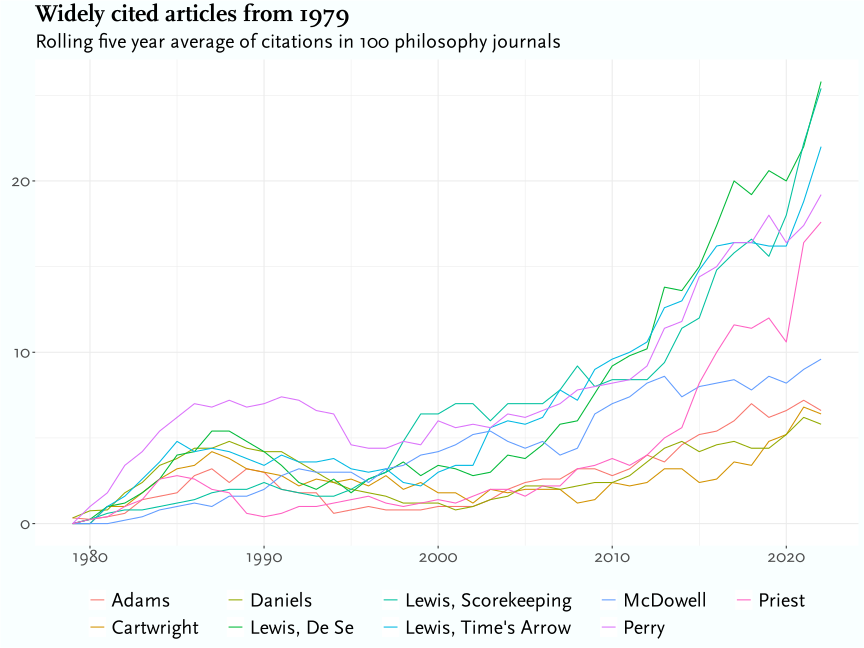
\includegraphics[keepaspectratio]{citations_files/figure-pdf/fig-citation-spaghetti-1979-1.pdf}}

}

\caption{\label{fig-citation-spaghetti-1979}Rolling five year average of
citation frequency for widely cited articles from 1979.}

\end{figure}%

\begin{figure}

\centering{

\pandocbounded{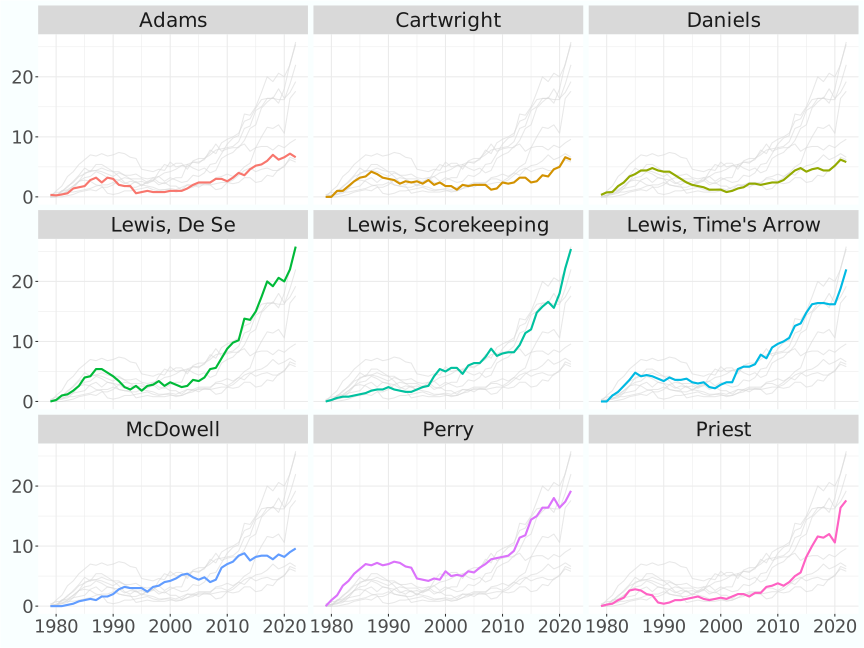
\includegraphics[keepaspectratio]{citations_files/figure-pdf/fig-citation-facet-1979-1.pdf}}

}

\caption{\label{fig-citation-facet-1979}Faceted version of
Figure~\ref{fig-citation-spaghetti-1979}.}

\end{figure}%

\newpage

\subsection{1980}\label{sec-s1980}

\subsubsection*{Widely Cited Articles}\label{widely-cited-articles-23}
\addcontentsline{toc}{subsubsection}{Widely Cited Articles}

\begin{enumerate}
\def\labelenumi{\arabic{enumi}.}
\tightlist
\item
  John Rawls (\citeproc{ref-WOSA1980KH88100001}{1980}) ``Kantian
  Constructivism in Moral Theory''
\item
  Martin Davies and Lloyd Humberstone
  (\citeproc{ref-WOSA1980KA40400001}{1980}) ``Two Notions of Necessity''
\item
  Hilary Putnam (\citeproc{ref-WOSA1980KJ75900004}{1980}) ``Models and
  Reality''
\item
  Jerrold Levinson (\citeproc{ref-WOSA1980JC98000001}{1980}) ``What a
  Musical Work Is''
\item
  Elliot Sober (\citeproc{ref-WOSA1980LE33500002}{1980}) ``Evolution,
  Population Thinking, and Essentialism''
\item
  Ruth Barcan Marcus (\citeproc{ref-WOSA1980JJ63300001}{1980}) ``Moral
  Dilemmas and Consistency''
\item
  David Lewis (\citeproc{ref-WOSA1980KX78600003}{1980}) ``Veridical
  Hallucination and Prosthetic Vision''
\item
  Norman Daniels (\citeproc{ref-WOSA1980JZ97600005}{1980}) ``Reflective
  Equilibrium and Archimedean Points''
\end{enumerate}

\subsubsection*{Citation Count}\label{sec-count-1980}
\addcontentsline{toc}{subsubsection}{Citation Count}


\begin{longtable}[]{@{}lrrr@{}}

\caption{\label{tbl-citation-count-1980}Citation count for widely cited
articles from 1980.}

\tabularnewline

\toprule\noalign{}
Article & All & Early & Late \\
\midrule\noalign{}
\endhead
\bottomrule\noalign{}
\endlastfoot
Rawls (\citeproc{ref-WOSA1980KH88100001}{1980})
& 202 & 56 & 61 \\
Davies and Humberstone (\citeproc{ref-WOSA1980KA40400001}{1980})
& 124 & 3 & 63 \\
Putnam (\citeproc{ref-WOSA1980KJ75900004}{1980})
& 115 & 21 & 55 \\
Levinson (\citeproc{ref-WOSA1980JC98000001}{1980})
& 103 & 10 & 58 \\
Sober (\citeproc{ref-WOSA1980LE33500002}{1980})
& 90 & 8 & 40 \\
Marcus (\citeproc{ref-WOSA1980JJ63300001}{1980})
& 88 & 24 & 36 \\
Lewis (\citeproc{ref-WOSA1980KX78600003}{1980})
& 82 & 9 & 45 \\
Daniels (\citeproc{ref-WOSA1980JZ97600005}{1980})
& 42 & 22 & 9 \\

\end{longtable}

\subsubsection*{Citation Rank}\label{sec-rank-1980}
\addcontentsline{toc}{subsubsection}{Citation Rank}


\begin{longtable}[]{@{}lrrr@{}}

\caption{\label{tbl-citation-rank-1980}Citation rank for widely cited
articles from 1980.}

\tabularnewline

\toprule\noalign{}
Article & Overall & Early & Late \\
\midrule\noalign{}
\endhead
\bottomrule\noalign{}
\endlastfoot
Rawls (\citeproc{ref-WOSA1980KH88100001}{1980})
& 1 & 1 & 2 \\
Davies and Humberstone (\citeproc{ref-WOSA1980KA40400001}{1980})
& 2 & 112 & 1 \\
Putnam (\citeproc{ref-WOSA1980KJ75900004}{1980})
& 3 & 4 & 4 \\
Levinson (\citeproc{ref-WOSA1980JC98000001}{1980})
& 4 & 11 & 3 \\
Sober (\citeproc{ref-WOSA1980LE33500002}{1980})
& 5 & 20 & 6 \\
Marcus (\citeproc{ref-WOSA1980JJ63300001}{1980})
& 6 & 2 & 7 \\
Lewis (\citeproc{ref-WOSA1980KX78600003}{1980})
& 7 & 13 & 5 \\
Daniels (\citeproc{ref-WOSA1980JZ97600005}{1980})
& 11 & 3 & 32 \\

\end{longtable}

\subsubsection*{Citation Trends}\label{sec-trends-1980}
\addcontentsline{toc}{subsubsection}{Citation Trends}

\begin{figure}

\centering{

\pandocbounded{\includegraphics[keepaspectratio]{citations_files/figure-pdf/fig-citation-spaghetti-1980-1.pdf}}

}

\caption{\label{fig-citation-spaghetti-1980}Rolling five year average of
citation frequency for widely cited articles from 1980.}

\end{figure}%

\begin{figure}

\centering{

\pandocbounded{\includegraphics[keepaspectratio]{citations_files/figure-pdf/fig-citation-facet-1980-1.pdf}}

}

\caption{\label{fig-citation-facet-1980}Faceted version of
Figure~\ref{fig-citation-spaghetti-1980}.}

\end{figure}%

\newpage

\subsection{1981}\label{sec-s1981}

\subsubsection*{Widely Cited Articles}\label{widely-cited-articles-24}
\addcontentsline{toc}{subsubsection}{Widely Cited Articles}

\begin{enumerate}
\def\labelenumi{\arabic{enumi}.}
\tightlist
\item
  Paul M. Churchland (\citeproc{ref-WOSA1981LD54600001}{1981})
  ``Eliminative Materialism and the Propositional Attitudes''
\item
  Larry Laudan (\citeproc{ref-WOSA1981LY92900002}{1981}) ``A Confutation
  of Convergent Realism''
\item
  Philip Kitcher (\citeproc{ref-WOSA1981NA08400001}{1981}) ``Explanatory
  Unification''
\item
  Jon Barwise and Robin Cooper (\citeproc{ref-WOSA1981LH67300001}{1981})
  ``Generalized Quantifiers and Natural-Language''
\item
  Ronald Dworkin (\citeproc{ref-WOSA1981MH21100001}{1981b}) ``What is
  Equality? Part 2: Equality of Resources''
\item
  David Lewis (\citeproc{ref-WOSA1981LW58400001}{1981}) ``Causal
  Decision Theory''
\item
  Peter van Inwagen (\citeproc{ref-WOSA1981LV91400003}{1981}) ``The
  Doctrine of Arbitrary Undetached Parts''
\item
  Ronald Dworkin (\citeproc{ref-WOSA1981LU74200001}{1981a}) ``What is
  Equality (I) Equality of Welfare''
\item
  John Dupré (\citeproc{ref-WOSA1981KZ94600003}{1981}) ``Natural Kinds
  and Biological Taxa''
\end{enumerate}

\subsubsection*{Citation Count}\label{sec-count-1981}
\addcontentsline{toc}{subsubsection}{Citation Count}


\begin{longtable}[]{@{}lrrr@{}}

\caption{\label{tbl-citation-count-1981}Citation count for widely cited
articles from 1981.}

\tabularnewline

\toprule\noalign{}
Article & All & Early & Late \\
\midrule\noalign{}
\endhead
\bottomrule\noalign{}
\endlastfoot
Churchland (\citeproc{ref-WOSA1981LD54600001}{1981})
& 281 & 59 & 113 \\
Laudan (\citeproc{ref-WOSA1981LY92900002}{1981})
& 275 & 28 & 142 \\
Kitcher (\citeproc{ref-WOSA1981NA08400001}{1981})
& 247 & 10 & 135 \\
Barwise and Cooper (\citeproc{ref-WOSA1981LH67300001}{1981})
& 222 & 39 & 87 \\
R. Dworkin (\citeproc{ref-WOSA1981MH21100001}{1981b})
& 208 & 25 & 79 \\
Lewis (\citeproc{ref-WOSA1981LW58400001}{1981})
& 173 & 35 & 99 \\
Inwagen (\citeproc{ref-WOSA1981LV91400003}{1981})
& 105 & 4 & 36 \\
R. Dworkin (\citeproc{ref-WOSA1981LU74200001}{1981a})
& 97 & 19 & 28 \\
Dupré (\citeproc{ref-WOSA1981KZ94600003}{1981})
& 93 & 16 & 26 \\

\end{longtable}

\subsubsection*{Citation Rank}\label{sec-rank-1981}
\addcontentsline{toc}{subsubsection}{Citation Rank}


\begin{longtable}[]{@{}lrrr@{}}

\caption{\label{tbl-citation-rank-1981}Citation rank for widely cited
articles from 1981.}

\tabularnewline

\toprule\noalign{}
Article & Overall & Early & Late \\
\midrule\noalign{}
\endhead
\bottomrule\noalign{}
\endlastfoot
Churchland (\citeproc{ref-WOSA1981LD54600001}{1981})
& 1 & 1 & 3 \\
Laudan (\citeproc{ref-WOSA1981LY92900002}{1981})
& 2 & 4 & 1 \\
Kitcher (\citeproc{ref-WOSA1981NA08400001}{1981})
& 3 & 17 & 2 \\
Barwise and Cooper (\citeproc{ref-WOSA1981LH67300001}{1981})
& 4 & 2 & 5 \\
R. Dworkin (\citeproc{ref-WOSA1981MH21100001}{1981b})
& 5 & 5 & 6 \\
Lewis (\citeproc{ref-WOSA1981LW58400001}{1981})
& 6 & 3 & 4 \\
Inwagen (\citeproc{ref-WOSA1981LV91400003}{1981})
& 7 & 86 & 11 \\
R. Dworkin (\citeproc{ref-WOSA1981LU74200001}{1981a})
& 8 & 6 & 14 \\
Dupré (\citeproc{ref-WOSA1981KZ94600003}{1981})
& 10 & 7 & 17 \\

\end{longtable}

\subsubsection*{Citation Trends}\label{sec-trends-1981}
\addcontentsline{toc}{subsubsection}{Citation Trends}

\begin{figure}

\centering{

\pandocbounded{\includegraphics[keepaspectratio]{citations_files/figure-pdf/fig-citation-spaghetti-1981-1.pdf}}

}

\caption{\label{fig-citation-spaghetti-1981}Rolling five year average of
citation frequency for widely cited articles from 1981.}

\end{figure}%

\begin{figure}

\centering{

\pandocbounded{\includegraphics[keepaspectratio]{citations_files/figure-pdf/fig-citation-facet-1981-1.pdf}}

}

\caption{\label{fig-citation-facet-1981}Faceted version of
Figure~\ref{fig-citation-spaghetti-1981}.}

\end{figure}%

\newpage

\subsection{1982}\label{sec-s1982}

\subsubsection*{Widely Cited Articles}\label{widely-cited-articles-25}
\addcontentsline{toc}{subsubsection}{Widely Cited Articles}

\begin{enumerate}
\def\labelenumi{\arabic{enumi}.}
\tightlist
\item
  Frank Jackson (\citeproc{ref-WOSA1982NH65300003}{1982})
  ``Epiphenomenal Qualia''
\item
  Susan Wolf (\citeproc{ref-WOSA1982PB73200001}{1982}) ``Moral Saints''
\item
  Elizabeth W. Prior, Robert Pargetter, and Frank Jackson
  (\citeproc{ref-WOSA1982NS00700005}{1982}) ``Three Theses About
  Dispositions''
\item
  Chris Swoyer (\citeproc{ref-WOSA1982PM91600001}{1982}) ``The Nature of
  Natural Laws''
\item
  Anil Gupta (\citeproc{ref-WOSA1982NW89300001}{1982}) ``Truth and
  Paradox''
\item
  David Lewis (\citeproc{ref-WOSA1982PN18900005}{1982}) ``Logic for
  Equivocators''
\item
  Jaegwon Kim (\citeproc{ref-WOSA1982NC90700004}{1982}) ``Psychophysical
  Supervenience''
\item
  Harry G. Frankfurt (\citeproc{ref-WOSA1982PX46500008}{1982}) ``The
  Importance of What We Care About''
\item
  Dudley Shapere (\citeproc{ref-WOSA1982PW68500001}{1982}) ``The Concept
  of Observation in Science and Philosophy''
\end{enumerate}

\subsubsection*{Citation Count}\label{sec-count-1982}
\addcontentsline{toc}{subsubsection}{Citation Count}


\begin{longtable}[]{@{}lrrr@{}}

\caption{\label{tbl-citation-count-1982}Citation count for widely cited
articles from 1982.}

\tabularnewline

\toprule\noalign{}
Article & All & Early & Late \\
\midrule\noalign{}
\endhead
\bottomrule\noalign{}
\endlastfoot
Jackson (\citeproc{ref-WOSA1982NH65300003}{1982})
& 473 & 25 & 238 \\
Wolf (\citeproc{ref-WOSA1982PB73200001}{1982})
& 161 & 18 & 74 \\
E. W. Prior, Pargetter, and Jackson(\citeproc{ref-WOSA1982NS00700005}{1982})
& 132 & 10 & 64 \\
Swoyer (\citeproc{ref-WOSA1982PM91600001}{1982})
& 107 & 7 & 46 \\
Gupta (\citeproc{ref-WOSA1982NW89300001}{1982})
& 91 & 25 & 39 \\
Lewis (\citeproc{ref-WOSA1982PN18900005}{1982})
& 89 & 4 & 74 \\
Kim (\citeproc{ref-WOSA1982NC90700004}{1982})
& 80 & 20 & 17 \\
Frankfurt (\citeproc{ref-WOSA1982PX46500008}{1982})
& 57 & 5 & 46 \\
Shapere (\citeproc{ref-WOSA1982PW68500001}{1982})
& 50 & 22 & 11 \\

\end{longtable}

\subsubsection*{Citation Rank}\label{sec-rank-1982}
\addcontentsline{toc}{subsubsection}{Citation Rank}


\begin{longtable}[]{@{}lrrr@{}}

\caption{\label{tbl-citation-rank-1982}Citation rank for widely cited
articles from 1982.}

\tabularnewline

\toprule\noalign{}
Article & Overall & Early & Late \\
\midrule\noalign{}
\endhead
\bottomrule\noalign{}
\endlastfoot
Jackson (\citeproc{ref-WOSA1982NH65300003}{1982})
& 1 & 2 & 1 \\
Wolf (\citeproc{ref-WOSA1982PB73200001}{1982})
& 2 & 7 & 2 \\
E. W. Prior, Pargetter, and Jackson(\citeproc{ref-WOSA1982NS00700005}{1982})
& 3 & 18 & 4 \\
Swoyer (\citeproc{ref-WOSA1982PM91600001}{1982})
& 4 & 42 & 5 \\
Gupta (\citeproc{ref-WOSA1982NW89300001}{1982})
& 5 & 2 & 7 \\
Lewis (\citeproc{ref-WOSA1982PN18900005}{1982})
& 6 & 93 & 2 \\
Kim (\citeproc{ref-WOSA1982NC90700004}{1982})
& 8 & 5 & 21 \\
Frankfurt (\citeproc{ref-WOSA1982PX46500008}{1982})
& 12 & 65 & 5 \\
Shapere (\citeproc{ref-WOSA1982PW68500001}{1982})
& 16 & 4 & 41 \\

\end{longtable}

\subsubsection*{Citation Trends}\label{sec-trends-1982}
\addcontentsline{toc}{subsubsection}{Citation Trends}

\begin{figure}

\centering{

\pandocbounded{\includegraphics[keepaspectratio]{citations_files/figure-pdf/fig-citation-spaghetti-1982-1.pdf}}

}

\caption{\label{fig-citation-spaghetti-1982}Rolling five year average of
citation frequency for widely cited articles from 1982.}

\end{figure}%

\begin{figure}

\centering{

\pandocbounded{\includegraphics[keepaspectratio]{citations_files/figure-pdf/fig-citation-facet-1982-1.pdf}}

}

\caption{\label{fig-citation-facet-1982}Faceted version of
Figure~\ref{fig-citation-spaghetti-1982}.}

\end{figure}%

\newpage

\subsection{1983}\label{sec-s1983}

\subsubsection*{Widely Cited Articles}\label{widely-cited-articles-26}
\addcontentsline{toc}{subsubsection}{Widely Cited Articles}

\begin{enumerate}
\def\labelenumi{\arabic{enumi}.}
\tightlist
\item
  David Lewis (\citeproc{ref-WOSA1983RR51600001}{1983}) ``New Work for a
  Theory of Universals''
\item
  Joseph Levine (\citeproc{ref-WOSA1983SU49200007}{1983}) ``Materialism
  and Qualia: The Explanatory Gap''
\item
  Gregory S. Kavka (\citeproc{ref-WOSA1983PX89100011}{1983}) ``The Toxin
  Puzzle''
\item
  Christine M. Korsgaard (\citeproc{ref-WOSA1983QN98800001}{1983}) ``Two
  Distinctions in Goodness''
\item
  Robert Brandom (\citeproc{ref-WOSA1983RV45200006}{1983}) ``Asserting''
\item
  Judith Jarvis Thomson (\citeproc{ref-WOSA1983QK97500001}{1983})
  ``Parthood and Identity Across Time''
\item
  Hilary Kornblith (\citeproc{ref-WOSA1983PZ01000002}{1983}) ``Justified
  Belief and Epistemically Responsible Action''
\item
  Alvin Plantinga (\citeproc{ref-WOSA1983QU18900001}{1983}) ``On
  Existentialism''
\item
  Ellery Eells and Elliot Sober
  (\citeproc{ref-WOSA1983QJ85300002}{1983}) ``Probabilistic Causality
  and the Question of Transitivity''
\end{enumerate}

\subsubsection*{Citation Count}\label{sec-count-1983}
\addcontentsline{toc}{subsubsection}{Citation Count}


\begin{longtable}[]{@{}lrrr@{}}

\caption{\label{tbl-citation-count-1983}Citation count for widely cited
articles from 1983.}

\tabularnewline

\toprule\noalign{}
Article & All & Early & Late \\
\midrule\noalign{}
\endhead
\bottomrule\noalign{}
\endlastfoot
Lewis (\citeproc{ref-WOSA1983RR51600001}{1983})
& 768 & 45 & 524 \\
Levine (\citeproc{ref-WOSA1983SU49200007}{1983})
& 214 & 3 & 107 \\
Kavka (\citeproc{ref-WOSA1983PX89100011}{1983})
& 167 & 15 & 87 \\
Korsgaard (\citeproc{ref-WOSA1983QN98800001}{1983})
& 140 & 6 & 91 \\
Brandom (\citeproc{ref-WOSA1983RV45200006}{1983})
& 106 & 6 & 65 \\
Thomson (\citeproc{ref-WOSA1983QK97500001}{1983})
& 97 & 7 & 34 \\
Kornblith (\citeproc{ref-WOSA1983PZ01000002}{1983})
& 84 & 21 & 41 \\
Plantinga (\citeproc{ref-WOSA1983QU18900001}{1983})
& 83 & 8 & 50 \\
Eells and Sober (\citeproc{ref-WOSA1983QJ85300002}{1983})
& 41 & 21 & 5 \\

\end{longtable}

\subsubsection*{Citation Rank}\label{sec-rank-1983}
\addcontentsline{toc}{subsubsection}{Citation Rank}


\begin{longtable}[]{@{}lrrr@{}}

\caption{\label{tbl-citation-rank-1983}Citation rank for widely cited
articles from 1983.}

\tabularnewline

\toprule\noalign{}
Article & Overall & Early & Late \\
\midrule\noalign{}
\endhead
\bottomrule\noalign{}
\endlastfoot
Lewis (\citeproc{ref-WOSA1983RR51600001}{1983})
& 1 & 1 & 1 \\
Levine (\citeproc{ref-WOSA1983SU49200007}{1983})
& 2 & 126 & 2 \\
Kavka (\citeproc{ref-WOSA1983PX89100011}{1983})
& 3 & 4 & 4 \\
Korsgaard (\citeproc{ref-WOSA1983QN98800001}{1983})
& 4 & 40 & 3 \\
Brandom (\citeproc{ref-WOSA1983RV45200006}{1983})
& 5 & 40 & 5 \\
Thomson (\citeproc{ref-WOSA1983QK97500001}{1983})
& 6 & 31 & 12 \\
Kornblith (\citeproc{ref-WOSA1983PZ01000002}{1983})
& 8 & 2 & 9 \\
Plantinga (\citeproc{ref-WOSA1983QU18900001}{1983})
& 9 & 22 & 6 \\
Eells and Sober (\citeproc{ref-WOSA1983QJ85300002}{1983})
& 16 & 2 & 72 \\

\end{longtable}

\subsubsection*{Citation Trends}\label{sec-trends-1983}
\addcontentsline{toc}{subsubsection}{Citation Trends}

\begin{figure}

\centering{

\pandocbounded{\includegraphics[keepaspectratio]{citations_files/figure-pdf/fig-citation-spaghetti-1983-1.pdf}}

}

\caption{\label{fig-citation-spaghetti-1983}Rolling five year average of
citation frequency for widely cited articles from 1983.}

\end{figure}%

\begin{figure}

\centering{

\pandocbounded{\includegraphics[keepaspectratio]{citations_files/figure-pdf/fig-citation-facet-1983-1.pdf}}

}

\caption{\label{fig-citation-facet-1983}Faceted version of
Figure~\ref{fig-citation-spaghetti-1983}.}

\end{figure}%

\newpage

\subsection{1984}\label{sec-s1984}

\subsubsection*{Widely Cited Articles}\label{widely-cited-articles-27}
\addcontentsline{toc}{subsubsection}{Widely Cited Articles}

\begin{enumerate}
\def\labelenumi{\arabic{enumi}.}
\tightlist
\item
  David Lewis (\citeproc{ref-WOSA1984TQ70900001}{1984}) ``Putnam's
  Paradox''
\item
  Bas C. van Fraassen (\citeproc{ref-WOSA1984SS95000001}{1984}) ``Belief
  and the Will''
\item
  Peter Railton (\citeproc{ref-WOSA1984SH40600002}{1984}) ``Alienation,
  Consequentialism, and the Demands of Morality''
\item
  George Boolos (\citeproc{ref-WOSA1984TE24500002}{1984}) ``To Be is To
  Be a Value of a Variable (Or To Be Some Values of Some Variables)''
\item
  Jaegwon Kim (\citeproc{ref-WOSA1984TV24600001}{1984}) ``Concepts of
  Supervenience''
\item
  Stewart Cohen (\citeproc{ref-WOSA1984TN86300001}{1984})
  ``Justification and Truth''
\item
  Philip Kitcher (\citeproc{ref-WOSA1984SZ73700006}{1984}) ``Species''
\item
  Kevin Mulligan, Peter Simons, and Barry Smith
  (\citeproc{ref-WOSA1984SE25700001}{1984}) ``Truth-Makers''
\item
  Jerry Fodor (\citeproc{ref-WOSA1984SL56000004}{1984}) ``Observation
  Reconsidered''
\end{enumerate}

\subsubsection*{Citation Count}\label{sec-count-1984}
\addcontentsline{toc}{subsubsection}{Citation Count}


\begin{longtable}[]{@{}lrrr@{}}

\caption{\label{tbl-citation-count-1984}Citation count for widely cited
articles from 1984.}

\tabularnewline

\toprule\noalign{}
Article & All & Early & Late \\
\midrule\noalign{}
\endhead
\bottomrule\noalign{}
\endlastfoot
Lewis (\citeproc{ref-WOSA1984TQ70900001}{1984})
& 229 & 18 & 130 \\
Fraassen (\citeproc{ref-WOSA1984SS95000001}{1984})
& 210 & 21 & 102 \\
Railton (\citeproc{ref-WOSA1984SH40600002}{1984})
& 201 & 19 & 114 \\
Boolos (\citeproc{ref-WOSA1984TE24500002}{1984})
& 198 & 14 & 108 \\
Kim (\citeproc{ref-WOSA1984TV24600001}{1984})
& 163 & 52 & 35 \\
S. Cohen (\citeproc{ref-WOSA1984TN86300001}{1984})
& 152 & 10 & 102 \\
Kitcher (\citeproc{ref-WOSA1984SZ73700006}{1984})
& 116 & 18 & 45 \\
Mulligan, Simons, and Smith (\citeproc{ref-WOSA1984SE25700001}{1984})
& 97 & 8 & 52 \\
Fodor (\citeproc{ref-WOSA1984SL56000004}{1984})
& 89 & 22 & 37 \\

\end{longtable}

\subsubsection*{Citation Rank}\label{sec-rank-1984}
\addcontentsline{toc}{subsubsection}{Citation Rank}


\begin{longtable}[]{@{}lrrr@{}}

\caption{\label{tbl-citation-rank-1984}Citation rank for widely cited
articles from 1984.}

\tabularnewline

\toprule\noalign{}
Article & Overall & Early & Late \\
\midrule\noalign{}
\endhead
\bottomrule\noalign{}
\endlastfoot
Lewis (\citeproc{ref-WOSA1984TQ70900001}{1984})
& 1 & 6 & 1 \\
Fraassen (\citeproc{ref-WOSA1984SS95000001}{1984})
& 2 & 3 & 4 \\
Railton (\citeproc{ref-WOSA1984SH40600002}{1984})
& 3 & 4 & 2 \\
Boolos (\citeproc{ref-WOSA1984TE24500002}{1984})
& 4 & 13 & 3 \\
Kim (\citeproc{ref-WOSA1984TV24600001}{1984})
& 5 & 1 & 13 \\
S. Cohen (\citeproc{ref-WOSA1984TN86300001}{1984})
& 6 & 21 & 4 \\
Kitcher (\citeproc{ref-WOSA1984SZ73700006}{1984})
& 7 & 6 & 9 \\
Mulligan, Simons, and Smith (\citeproc{ref-WOSA1984SE25700001}{1984})
& 9 & 30 & 6 \\
Fodor (\citeproc{ref-WOSA1984SL56000004}{1984})
& 10 & 2 & 11 \\

\end{longtable}

\subsubsection*{Citation Trends}\label{sec-trends-1984}
\addcontentsline{toc}{subsubsection}{Citation Trends}

\begin{figure}

\centering{

\pandocbounded{\includegraphics[keepaspectratio]{citations_files/figure-pdf/fig-citation-spaghetti-1984-1.pdf}}

}

\caption{\label{fig-citation-spaghetti-1984}Rolling five year average of
citation frequency for widely cited articles from 1984.}

\end{figure}%

\begin{figure}

\centering{

\pandocbounded{\includegraphics[keepaspectratio]{citations_files/figure-pdf/fig-citation-facet-1984-1.pdf}}

}

\caption{\label{fig-citation-facet-1984}Faceted version of
Figure~\ref{fig-citation-spaghetti-1984}.}

\end{figure}%

\newpage

\subsection{1985}\label{sec-s1985}

\subsubsection*{Widely Cited Articles}\label{widely-cited-articles-28}
\addcontentsline{toc}{subsubsection}{Widely Cited Articles}

\begin{enumerate}
\def\labelenumi{\arabic{enumi}.}
\tightlist
\item
  Carlos E. Alchourrón, Peter Gärdenfors, and David Makinson
  (\citeproc{ref-WOSA1985AKA2200025}{1985}) ``On the Logic of Theory
  Change: Partial Meet Contraction and Revision Functions''
\item
  Richard Feldman and Earl Conee
  (\citeproc{ref-WOSA1985ANT6600002}{1985}) ``Evidentialism''
\item
  John Hardwig (\citeproc{ref-WOSA1985ALK4200001}{1985}) ``Epistemic
  Dependence''
\item
  Ernan McMullin (\citeproc{ref-WOSA1985ARQ5600003}{1985}) ``Galilean
  Idealization''
\item
  Vann McGee (\citeproc{ref-WOSA1985AQZ7400002}{1985}) ``A
  Counterexample To Modus Ponens''
\item
  John Rawls (\citeproc{ref-WOSA1985APA8500001}{1985}) ``Justice as
  Fairness: Political Not Metaphysical''
\item
  William P. Alston (\citeproc{ref-WOSA1985AML6300004}{1985}) ``Concepts
  of Epistemic Justification''
\item
  Richard Feldman (\citeproc{ref-WOSA1985APJ3700001}{1985})
  ``Reliability and Justification''
\item
  Paul M. Churchland (\citeproc{ref-WOSA1985AAC6100002}{1985})
  ``Reduction, Qualia, and the Direct Introspection of Brain States''
\end{enumerate}

\subsubsection*{Citation Count}\label{sec-count-1985}
\addcontentsline{toc}{subsubsection}{Citation Count}


\begin{longtable}[]{@{}lrrr@{}}

\caption{\label{tbl-citation-count-1985}Citation count for widely cited
articles from 1985.}

\tabularnewline

\toprule\noalign{}
Article & All & Early & Late \\
\midrule\noalign{}
\endhead
\bottomrule\noalign{}
\endlastfoot
Alchourrón, Gärdenfors, and Makinson(\citeproc{ref-WOSA1985AKA2200025}{1985})
& 264 & 23 & 120 \\
Feldman and Conee (\citeproc{ref-WOSA1985ANT6600002}{1985})
& 174 & 6 & 119 \\
Hardwig (\citeproc{ref-WOSA1985ALK4200001}{1985})
& 155 & 10 & 100 \\
McMullin (\citeproc{ref-WOSA1985ARQ5600003}{1985})
& 142 & 4 & 89 \\
McGee (\citeproc{ref-WOSA1985AQZ7400002}{1985})
& 132 & 8 & 98 \\
Rawls (\citeproc{ref-WOSA1985APA8500001}{1985})
& 105 & 48 & 25 \\
Alston (\citeproc{ref-WOSA1985AML6300004}{1985})
& 92 & 18 & 44 \\
Feldman (\citeproc{ref-WOSA1985APJ3700001}{1985})
& 78 & 20 & 29 \\
Churchland (\citeproc{ref-WOSA1985AAC6100002}{1985})
& 74 & 22 & 16 \\

\end{longtable}

\subsubsection*{Citation Rank}\label{sec-rank-1985}
\addcontentsline{toc}{subsubsection}{Citation Rank}


\begin{longtable}[]{@{}lrrr@{}}

\caption{\label{tbl-citation-rank-1985}Citation rank for widely cited
articles from 1985.}

\tabularnewline

\toprule\noalign{}
Article & Overall & Early & Late \\
\midrule\noalign{}
\endhead
\bottomrule\noalign{}
\endlastfoot
Alchourrón, Gärdenfors, and Makinson(\citeproc{ref-WOSA1985AKA2200025}{1985})
& 1 & 2 & 1 \\
Feldman and Conee (\citeproc{ref-WOSA1985ANT6600002}{1985})
& 2 & 40 & 2 \\
Hardwig (\citeproc{ref-WOSA1985ALK4200001}{1985})
& 3 & 12 & 3 \\
McMullin (\citeproc{ref-WOSA1985ARQ5600003}{1985})
& 4 & 80 & 5 \\
McGee (\citeproc{ref-WOSA1985AQZ7400002}{1985})
& 5 & 19 & 4 \\
Rawls (\citeproc{ref-WOSA1985APA8500001}{1985})
& 7 & 1 & 12 \\
Alston (\citeproc{ref-WOSA1985AML6300004}{1985})
& 8 & 5 & 8 \\
Feldman (\citeproc{ref-WOSA1985APJ3700001}{1985})
& 10 & 4 & 10 \\
Churchland (\citeproc{ref-WOSA1985AAC6100002}{1985})
& 11 & 3 & 23 \\

\end{longtable}

\subsubsection*{Citation Trends}\label{sec-trends-1985}
\addcontentsline{toc}{subsubsection}{Citation Trends}

\begin{figure}

\centering{

\pandocbounded{\includegraphics[keepaspectratio]{citations_files/figure-pdf/fig-citation-spaghetti-1985-1.pdf}}

}

\caption{\label{fig-citation-spaghetti-1985}Rolling five year average of
citation frequency for widely cited articles from 1985.}

\end{figure}%

\begin{figure}

\centering{

\pandocbounded{\includegraphics[keepaspectratio]{citations_files/figure-pdf/fig-citation-facet-1985-1.pdf}}

}

\caption{\label{fig-citation-facet-1985}Faceted version of
Figure~\ref{fig-citation-spaghetti-1985}.}

\end{figure}%

\newpage

\subsection{1986}\label{sec-s1986}

\subsubsection*{Widely Cited Articles}\label{widely-cited-articles-29}
\addcontentsline{toc}{subsubsection}{Widely Cited Articles}

\begin{enumerate}
\def\labelenumi{\arabic{enumi}.}
\tightlist
\item
  Peter Railton (\citeproc{ref-WOSA1986C044900001}{1986}) ``Moral
  Realism''
\item
  Tyler Burge (\citeproc{ref-WOSA1986AYX3200001}{1986a}) ``Individualism
  and Psychology''
\item
  Annette Baier (\citeproc{ref-WOSA1986AYY3900001}{1986}) ``Trust and
  Antitrust''
\item
  Christine M. Korsgaard (\citeproc{ref-WOSA1986AYQ1300001}{1986})
  ``Skepticism About Practical Reason''
\item
  David M. Rosenthal (\citeproc{ref-WOSA1986C316000003}{1986}) ``Two
  Concepts of Consciousness''
\item
  Frank Jackson and Robert Pargetter
  (\citeproc{ref-WOSA1986C044900003}{1986}) ``Oughts, Options, and
  Actualism''
\item
  Tyler Burge (\citeproc{ref-WOSA1986F231300001}{1986b}) ``Intellectual
  Norms and Foundations of Mind''
\item
  Ruth Garrett Millikan (\citeproc{ref-WOSA1986AYX3200002}{1986})
  ``Thoughts Without Laws, Cognitive Science With Content''
\end{enumerate}

\subsubsection*{Citation Count}\label{sec-count-1986}
\addcontentsline{toc}{subsubsection}{Citation Count}


\begin{longtable}[]{@{}lrrr@{}}

\caption{\label{tbl-citation-count-1986}Citation count for widely cited
articles from 1986.}

\tabularnewline

\toprule\noalign{}
Article & All & Early & Late \\
\midrule\noalign{}
\endhead
\bottomrule\noalign{}
\endlastfoot
Railton (\citeproc{ref-WOSA1986C044900001}{1986})
& 240 & 38 & 116 \\
Burge (\citeproc{ref-WOSA1986AYX3200001}{1986a})
& 186 & 60 & 52 \\
Baier (\citeproc{ref-WOSA1986AYY3900001}{1986})
& 172 & 24 & 107 \\
Korsgaard (\citeproc{ref-WOSA1986AYQ1300001}{1986})
& 155 & 15 & 75 \\
Rosenthal (\citeproc{ref-WOSA1986C316000003}{1986})
& 125 & 16 & 47 \\
Jackson and Pargetter (\citeproc{ref-WOSA1986C044900003}{1986})
& 103 & 10 & 69 \\
Burge (\citeproc{ref-WOSA1986F231300001}{1986b})
& 103 & 17 & 39 \\
Millikan (\citeproc{ref-WOSA1986AYX3200002}{1986})
& 42 & 23 & 3 \\

\end{longtable}

\subsubsection*{Citation Rank}\label{sec-rank-1986}
\addcontentsline{toc}{subsubsection}{Citation Rank}


\begin{longtable}[]{@{}lrrr@{}}

\caption{\label{tbl-citation-rank-1986}Citation rank for widely cited
articles from 1986.}

\tabularnewline

\toprule\noalign{}
Article & Overall & Early & Late \\
\midrule\noalign{}
\endhead
\bottomrule\noalign{}
\endlastfoot
Railton (\citeproc{ref-WOSA1986C044900001}{1986})
& 1 & 2 & 1 \\
Burge (\citeproc{ref-WOSA1986AYX3200001}{1986a})
& 2 & 1 & 5 \\
Baier (\citeproc{ref-WOSA1986AYY3900001}{1986})
& 3 & 3 & 2 \\
Korsgaard (\citeproc{ref-WOSA1986AYQ1300001}{1986})
& 4 & 8 & 3 \\
Rosenthal (\citeproc{ref-WOSA1986C316000003}{1986})
& 5 & 7 & 6 \\
Jackson and Pargetter (\citeproc{ref-WOSA1986C044900003}{1986})
& 6 & 19 & 4 \\
Burge (\citeproc{ref-WOSA1986F231300001}{1986b})
& 6 & 5 & 9 \\
Millikan (\citeproc{ref-WOSA1986AYX3200002}{1986})
& 22 & 4 & 139 \\

\end{longtable}

\subsubsection*{Citation Trends}\label{sec-trends-1986}
\addcontentsline{toc}{subsubsection}{Citation Trends}

\begin{figure}

\centering{

\pandocbounded{\includegraphics[keepaspectratio]{citations_files/figure-pdf/fig-citation-spaghetti-1986-1.pdf}}

}

\caption{\label{fig-citation-spaghetti-1986}Rolling five year average of
citation frequency for widely cited articles from 1986.}

\end{figure}%

\begin{figure}

\centering{

\pandocbounded{\includegraphics[keepaspectratio]{citations_files/figure-pdf/fig-citation-facet-1986-1.pdf}}

}

\caption{\label{fig-citation-facet-1986}Faceted version of
Figure~\ref{fig-citation-spaghetti-1986}.}

\end{figure}%

\newpage

\subsection{1987}\label{sec-s1987}

\subsubsection*{Widely Cited Articles}\label{widely-cited-articles-30}
\addcontentsline{toc}{subsubsection}{Widely Cited Articles}

\begin{enumerate}
\def\labelenumi{\arabic{enumi}.}
\tightlist
\item
  M Smith (\citeproc{ref-WOSA1987F993300003}{1987}) ``The Humean Theory
  of Motivation''
\item
  Harry G. Frankfurt (\citeproc{ref-WOSA1987M543000002}{1987})
  ``Equality as a Moral Ideal''
\item
  John Bigelow and Robert Pargetter
  (\citeproc{ref-WOSA1987G947600001}{1987}) ``Functions''
\item
  John Earman and John Norton (\citeproc{ref-WOSA1987M488500005}{1987})
  ``What Price Spacetime Substantivalism: The Hole Story''
\item
  DW Stampe (\citeproc{ref-WOSA1987J665800001}{1987}) ``The Authority of
  Desire''
\item
  LS Temkin (\citeproc{ref-WOSA1987H340500002}{1987}) ``Intransitivity
  and the Mere Addition Paradox''
\item
  Thomas Nagel (\citeproc{ref-WOSA1987J379200001}{1987}) ``Moral
  Conflict and Political Legitimacy''
\item
  M Gilbert (\citeproc{ref-WOSA1987K730800008}{1987}) ``Modeling
  Collective Belief''
\item
  Larry Laudan (\citeproc{ref-WOSA1987F902200002}{1987}) ``Progress or
  Rationality: The Prospects for Normative Naturalism''
\end{enumerate}

\subsubsection*{Citation Count}\label{sec-count-1987}
\addcontentsline{toc}{subsubsection}{Citation Count}


\begin{longtable}[]{@{}lrrr@{}}

\caption{\label{tbl-citation-count-1987}Citation count for widely cited
articles from 1987.}

\tabularnewline

\toprule\noalign{}
Article & All & Early & Late \\
\midrule\noalign{}
\endhead
\bottomrule\noalign{}
\endlastfoot
M. Smith (\citeproc{ref-WOSA1987F993300003}{1987})
& 127 & 20 & 65 \\
Frankfurt (\citeproc{ref-WOSA1987M543000002}{1987})
& 94 & 1 & 62 \\
Bigelow and Pargetter (\citeproc{ref-WOSA1987G947600001}{1987})
& 92 & 23 & 33 \\
Earman and Norton (\citeproc{ref-WOSA1987M488500005}{1987})
& 83 & 21 & 36 \\
Stampe (\citeproc{ref-WOSA1987J665800001}{1987})
& 80 & 6 & 54 \\
Temkin (\citeproc{ref-WOSA1987H340500002}{1987})
& 76 & 4 & 43 \\
Nagel (\citeproc{ref-WOSA1987J379200001}{1987})
& 71 & 17 & 25 \\
Gilbert (\citeproc{ref-WOSA1987K730800008}{1987})
& 67 & 5 & 50 \\
Laudan (\citeproc{ref-WOSA1987F902200002}{1987})
& 54 & 28 & 10 \\

\end{longtable}

\subsubsection*{Citation Rank}\label{sec-rank-1987}
\addcontentsline{toc}{subsubsection}{Citation Rank}


\begin{longtable}[]{@{}lrrr@{}}

\caption{\label{tbl-citation-rank-1987}Citation rank for widely cited
articles from 1987.}

\tabularnewline

\toprule\noalign{}
Article & Overall & Early & Late \\
\midrule\noalign{}
\endhead
\bottomrule\noalign{}
\endlastfoot
M. Smith (\citeproc{ref-WOSA1987F993300003}{1987})
& 1 & 4 & 1 \\
Frankfurt (\citeproc{ref-WOSA1987M543000002}{1987})
& 2 & 304 & 2 \\
Bigelow and Pargetter (\citeproc{ref-WOSA1987G947600001}{1987})
& 3 & 2 & 7 \\
Earman and Norton (\citeproc{ref-WOSA1987M488500005}{1987})
& 4 & 3 & 6 \\
Stampe (\citeproc{ref-WOSA1987J665800001}{1987})
& 5 & 40 & 3 \\
Temkin (\citeproc{ref-WOSA1987H340500002}{1987})
& 6 & 74 & 5 \\
Nagel (\citeproc{ref-WOSA1987J379200001}{1987})
& 7 & 5 & 10 \\
Gilbert (\citeproc{ref-WOSA1987K730800008}{1987})
& 9 & 54 & 4 \\
Laudan (\citeproc{ref-WOSA1987F902200002}{1987})
& 13 & 1 & 37 \\

\end{longtable}

\subsubsection*{Citation Trends}\label{sec-trends-1987}
\addcontentsline{toc}{subsubsection}{Citation Trends}

\begin{figure}

\centering{

\pandocbounded{\includegraphics[keepaspectratio]{citations_files/figure-pdf/fig-citation-spaghetti-1987-1.pdf}}

}

\caption{\label{fig-citation-spaghetti-1987}Rolling five year average of
citation frequency for widely cited articles from 1987.}

\end{figure}%

\begin{figure}

\centering{

\pandocbounded{\includegraphics[keepaspectratio]{citations_files/figure-pdf/fig-citation-facet-1987-1.pdf}}

}

\caption{\label{fig-citation-facet-1987}Faceted version of
Figure~\ref{fig-citation-spaghetti-1987}.}

\end{figure}%

\newpage

\subsection{1988}\label{sec-s1988}

\subsubsection*{Widely Cited Articles}\label{widely-cited-articles-31}
\addcontentsline{toc}{subsubsection}{Widely Cited Articles}

\begin{enumerate}
\def\labelenumi{\arabic{enumi}.}
\tightlist
\item
  Tyler Burge (\citeproc{ref-WOSA1988R020000007}{1988}) ``Individualism
  and Self-Knowledge''
\item
  James Bogen and James Woodward
  (\citeproc{ref-WOSA1988N938600001}{1988}) ``Saving the Phenomena''
\item
  A Grove (\citeproc{ref-WOSA1988M958800004}{1988}) ``Two Modelings for
  Theory Change''
\item
  K Sterelny and Philip Kitcher
  (\citeproc{ref-WOSA1988P217100001}{1988}) ``The Return of the Gene''
\item
  S Kagan (\citeproc{ref-WOSA1988Q913800001}{1988}) ``The Additive
  Fallacy''
\item
  William P. Alston (\citeproc{ref-WOSA1988M863300002}{1988}) ``An
  Internalist Externalism''
\item
  David Lewis (\citeproc{ref-WOSA1988P549200001}{1988}) ``Desire as
  Belief''
\item
  Frank Jackson and Philip Pettit
  (\citeproc{ref-WOSA1988P549200004}{1988}) ``Functionalism and Broad
  Content''
\item
  John Rawls (\citeproc{ref-WOSA1988Q394000001}{1988}) ``The Priority of
  Right and Ideas of the Good''
\end{enumerate}

\subsubsection*{Citation Count}\label{sec-count-1988}
\addcontentsline{toc}{subsubsection}{Citation Count}


\begin{longtable}[]{@{}lrrr@{}}

\caption{\label{tbl-citation-count-1988}Citation count for widely cited
articles from 1988.}

\tabularnewline

\toprule\noalign{}
Article & All & Early & Late \\
\midrule\noalign{}
\endhead
\bottomrule\noalign{}
\endlastfoot
Burge (\citeproc{ref-WOSA1988R020000007}{1988})
& 174 & 27 & 53 \\
Bogen and Woodward (\citeproc{ref-WOSA1988N938600001}{1988})
& 158 & 20 & 83 \\
Grove (\citeproc{ref-WOSA1988M958800004}{1988})
& 109 & 6 & 55 \\
Sterelny and Kitcher (\citeproc{ref-WOSA1988P217100001}{1988})
& 83 & 21 & 19 \\
Kagan (\citeproc{ref-WOSA1988Q913800001}{1988})
& 76 & 11 & 39 \\
Alston (\citeproc{ref-WOSA1988M863300002}{1988})
& 70 & 7 & 44 \\
Lewis (\citeproc{ref-WOSA1988P549200001}{1988})
& 68 & 13 & 40 \\
Jackson and Pettit (\citeproc{ref-WOSA1988P549200004}{1988})
& 68 & 34 & 9 \\
Rawls (\citeproc{ref-WOSA1988Q394000001}{1988})
& 45 & 27 & 13 \\

\end{longtable}

\subsubsection*{Citation Rank}\label{sec-rank-1988}
\addcontentsline{toc}{subsubsection}{Citation Rank}


\begin{longtable}[]{@{}lrrr@{}}

\caption{\label{tbl-citation-rank-1988}Citation rank for widely cited
articles from 1988.}

\tabularnewline

\toprule\noalign{}
Article & Overall & Early & Late \\
\midrule\noalign{}
\endhead
\bottomrule\noalign{}
\endlastfoot
Burge (\citeproc{ref-WOSA1988R020000007}{1988})
& 1 & 2 & 3 \\
Bogen and Woodward (\citeproc{ref-WOSA1988N938600001}{1988})
& 2 & 5 & 1 \\
Grove (\citeproc{ref-WOSA1988M958800004}{1988})
& 3 & 49 & 2 \\
Sterelny and Kitcher (\citeproc{ref-WOSA1988P217100001}{1988})
& 4 & 4 & 17 \\
Kagan (\citeproc{ref-WOSA1988Q913800001}{1988})
& 5 & 18 & 6 \\
Alston (\citeproc{ref-WOSA1988M863300002}{1988})
& 6 & 37 & 4 \\
Lewis (\citeproc{ref-WOSA1988P549200001}{1988})
& 8 & 12 & 5 \\
Jackson and Pettit (\citeproc{ref-WOSA1988P549200004}{1988})
& 8 & 1 & 51 \\
Rawls (\citeproc{ref-WOSA1988Q394000001}{1988})
& 18 & 2 & 37 \\

\end{longtable}

\subsubsection*{Citation Trends}\label{sec-trends-1988}
\addcontentsline{toc}{subsubsection}{Citation Trends}

\begin{figure}

\centering{

\pandocbounded{\includegraphics[keepaspectratio]{citations_files/figure-pdf/fig-citation-spaghetti-1988-1.pdf}}

}

\caption{\label{fig-citation-spaghetti-1988}Rolling five year average of
citation frequency for widely cited articles from 1988.}

\end{figure}%

\begin{figure}

\centering{

\pandocbounded{\includegraphics[keepaspectratio]{citations_files/figure-pdf/fig-citation-facet-1988-1.pdf}}

}

\caption{\label{fig-citation-facet-1988}Faceted version of
Figure~\ref{fig-citation-spaghetti-1988}.}

\end{figure}%

\newpage

\subsection{1989}\label{sec-s1989}

\subsubsection*{Widely Cited Articles}\label{widely-cited-articles-32}
\addcontentsline{toc}{subsubsection}{Widely Cited Articles}

\begin{enumerate}
\def\labelenumi{\arabic{enumi}.}
\tightlist
\item
  G. A. Cohen (\citeproc{ref-WOSA1989AE70300010}{1989}) ``On the
  Currency of Egalitarian Justice''
\item
  Ruth Garrett Millikan (\citeproc{ref-WOSA1989AA09400006}{1989b}) ``In
  Defense of Proper Functions''
\item
  Ruth Garrett Millikan (\citeproc{ref-WOSA1989U850300001}{1989a})
  ``Biosemantics''
\item
  Paul A. Boghossian and J. David Velleman
  (\citeproc{ref-WOSA1989T231400005}{1989}) ``Color as a Secondary
  Quality''
\item
  RJ Arneson (\citeproc{ref-WOSA1989U808000004}{1989}) ``Equality and
  Equal Opportunity for Welfare''
\item
  Paul A. Boghossian (\citeproc{ref-WOSA1989CA94000002}{1989}) ``The
  Rule-Following Considerations''
\item
  M Crimmins and John Perry (\citeproc{ref-WOSA1989CF70700001}{1989})
  ``The Prince and the Phone Booth: Reporting Puzzling Beliefs''
\item
  D Marquis (\citeproc{ref-WOSA1989U039600002}{1989}) ``Why Abortion is
  Immoral''
\item
  WS Quinn (\citeproc{ref-WOSA1989AV72300002}{1989}) ``Actions,
  Intentions, and Consequences: The Doctrine of Double Effect''
\end{enumerate}

\subsubsection*{Citation Count}\label{sec-count-1989}
\addcontentsline{toc}{subsubsection}{Citation Count}


\begin{longtable}[]{@{}lrrr@{}}

\caption{\label{tbl-citation-count-1989}Citation count for widely cited
articles from 1989.}

\tabularnewline

\toprule\noalign{}
Article & All & Early & Late \\
\midrule\noalign{}
\endhead
\bottomrule\noalign{}
\endlastfoot
G. A. Cohen (\citeproc{ref-WOSA1989AE70300010}{1989})
& 271 & 32 & 117 \\
Millikan (\citeproc{ref-WOSA1989AA09400006}{1989b})
& 183 & 40 & 88 \\
Millikan (\citeproc{ref-WOSA1989U850300001}{1989a})
& 180 & 39 & 94 \\
P. A. Boghossian and Velleman (\citeproc{ref-WOSA1989T231400005}{1989})
& 152 & 25 & 67 \\
Arneson (\citeproc{ref-WOSA1989U808000004}{1989})
& 152 & 14 & 72 \\
P. A. Boghossian (\citeproc{ref-WOSA1989CA94000002}{1989})
& 114 & 19 & 44 \\
Crimmins and Perry (\citeproc{ref-WOSA1989CF70700001}{1989})
& 107 & 34 & 43 \\
Marquis (\citeproc{ref-WOSA1989U039600002}{1989})
& 95 & 7 & 50 \\
Quinn (\citeproc{ref-WOSA1989AV72300002}{1989})
& 84 & 16 & 50 \\

\end{longtable}

\subsubsection*{Citation Rank}\label{sec-rank-1989}
\addcontentsline{toc}{subsubsection}{Citation Rank}


\begin{longtable}[]{@{}lrrr@{}}

\caption{\label{tbl-citation-rank-1989}Citation rank for widely cited
articles from 1989.}

\tabularnewline

\toprule\noalign{}
Article & Overall & Early & Late \\
\midrule\noalign{}
\endhead
\bottomrule\noalign{}
\endlastfoot
G. A. Cohen (\citeproc{ref-WOSA1989AE70300010}{1989})
& 1 & 4 & 1 \\
Millikan (\citeproc{ref-WOSA1989AA09400006}{1989b})
& 2 & 1 & 3 \\
Millikan (\citeproc{ref-WOSA1989U850300001}{1989a})
& 3 & 2 & 2 \\
P. A. Boghossian and Velleman (\citeproc{ref-WOSA1989T231400005}{1989})
& 4 & 5 & 5 \\
Arneson (\citeproc{ref-WOSA1989U808000004}{1989})
& 4 & 11 & 4 \\
P. A. Boghossian (\citeproc{ref-WOSA1989CA94000002}{1989})
& 6 & 7 & 10 \\
Crimmins and Perry (\citeproc{ref-WOSA1989CF70700001}{1989})
& 7 & 3 & 11 \\
Marquis (\citeproc{ref-WOSA1989U039600002}{1989})
& 9 & 37 & 6 \\
Quinn (\citeproc{ref-WOSA1989AV72300002}{1989})
& 10 & 9 & 6 \\

\end{longtable}

\subsubsection*{Citation Trends}\label{sec-trends-1989}
\addcontentsline{toc}{subsubsection}{Citation Trends}

\begin{figure}

\centering{

\pandocbounded{\includegraphics[keepaspectratio]{citations_files/figure-pdf/fig-citation-spaghetti-1989-1.pdf}}

}

\caption{\label{fig-citation-spaghetti-1989}Rolling five year average of
citation frequency for widely cited articles from 1989.}

\end{figure}%

\begin{figure}

\centering{

\pandocbounded{\includegraphics[keepaspectratio]{citations_files/figure-pdf/fig-citation-facet-1989-1.pdf}}

}

\caption{\label{fig-citation-facet-1989}Faceted version of
Figure~\ref{fig-citation-spaghetti-1989}.}

\end{figure}%

\newpage

\subsection{1990}\label{sec-s1990}

\subsubsection*{Widely Cited Articles}\label{widely-cited-articles-33}
\addcontentsline{toc}{subsubsection}{Widely Cited Articles}

\begin{enumerate}
\def\labelenumi{\arabic{enumi}.}
\tightlist
\item
  Philip Kitcher (\citeproc{ref-WOSA1990CH71200001}{1990}) ``The
  Division of Cognitive Labor''
\item
  Frank Jackson and Philip Pettit
  (\citeproc{ref-WOSA1990CR32400008}{1990}) ``Program Explanation: A
  General Perspective''
\item
  Donald Davidson (\citeproc{ref-WOSA1990EQ84600001}{1990}) ``The
  Structure and Content of Truth''
\item
  Gideon Rosen (\citeproc{ref-WOSA1990DR99100001}{1990}) ``Modal
  Fictionalism''
\item
  Tim Crane and D. H. Mellor (\citeproc{ref-WOSA1990DA14600002}{1990})
  ``There is No Question of Physicalism''
\item
  J Dreier (\citeproc{ref-WOSA1990EK23400001}{1990}) ``Internalism and
  Speaker Relativism''
\item
  J Vogel (\citeproc{ref-WOSA1990EF94500012}{1990}) ``Cartesian
  Skepticism and Inference To the Best Explanation''
\item
  Jaegwon Kim (\citeproc{ref-WOSA1990FU75100001}{1990}) ``Supervenience
  as a Philosophical Concept''
\item
  Graeme Forbes (\citeproc{ref-WOSA1990EB39300002}{1990}) ``The
  Indispensability of Sinn''
\end{enumerate}

\subsubsection*{Citation Count}\label{sec-count-1990}
\addcontentsline{toc}{subsubsection}{Citation Count}


\begin{longtable}[]{@{}lrrr@{}}

\caption{\label{tbl-citation-count-1990}Citation count for widely cited
articles from 1990.}

\tabularnewline

\toprule\noalign{}
Article & All & Early & Late \\
\midrule\noalign{}
\endhead
\bottomrule\noalign{}
\endlastfoot
Kitcher (\citeproc{ref-WOSA1990CH71200001}{1990})
& 171 & 24 & 118 \\
Jackson and Pettit (\citeproc{ref-WOSA1990CR32400008}{1990})
& 126 & 19 & 60 \\
Davidson (\citeproc{ref-WOSA1990EQ84600001}{1990})
& 123 & 44 & 32 \\
Rosen (\citeproc{ref-WOSA1990DR99100001}{1990})
& 108 & 21 & 44 \\
Crane and Mellor (\citeproc{ref-WOSA1990DA14600002}{1990})
& 100 & 35 & 30 \\
Dreier (\citeproc{ref-WOSA1990EK23400001}{1990})
& 87 & 10 & 42 \\
Vogel (\citeproc{ref-WOSA1990EF94500012}{1990})
& 75 & 8 & 46 \\
Kim (\citeproc{ref-WOSA1990FU75100001}{1990})
& 61 & 25 & 22 \\
Forbes (\citeproc{ref-WOSA1990EB39300002}{1990})
& 42 & 23 & 8 \\

\end{longtable}

\subsubsection*{Citation Rank}\label{sec-rank-1990}
\addcontentsline{toc}{subsubsection}{Citation Rank}


\begin{longtable}[]{@{}lrrr@{}}

\caption{\label{tbl-citation-rank-1990}Citation rank for widely cited
articles from 1990.}

\tabularnewline

\toprule\noalign{}
Article & Overall & Early & Late \\
\midrule\noalign{}
\endhead
\bottomrule\noalign{}
\endlastfoot
Kitcher (\citeproc{ref-WOSA1990CH71200001}{1990})
& 1 & 4 & 1 \\
Jackson and Pettit (\citeproc{ref-WOSA1990CR32400008}{1990})
& 2 & 9 & 2 \\
Davidson (\citeproc{ref-WOSA1990EQ84600001}{1990})
& 3 & 1 & 7 \\
Rosen (\citeproc{ref-WOSA1990DR99100001}{1990})
& 4 & 7 & 4 \\
Crane and Mellor (\citeproc{ref-WOSA1990DA14600002}{1990})
& 5 & 2 & 9 \\
Dreier (\citeproc{ref-WOSA1990EK23400001}{1990})
& 6 & 19 & 5 \\
Vogel (\citeproc{ref-WOSA1990EF94500012}{1990})
& 8 & 29 & 3 \\
Kim (\citeproc{ref-WOSA1990FU75100001}{1990})
& 11 & 3 & 16 \\
Forbes (\citeproc{ref-WOSA1990EB39300002}{1990})
& 21 & 5 & 53 \\

\end{longtable}

\subsubsection*{Citation Trends}\label{sec-trends-1990}
\addcontentsline{toc}{subsubsection}{Citation Trends}

\begin{figure}

\centering{

\pandocbounded{\includegraphics[keepaspectratio]{citations_files/figure-pdf/fig-citation-spaghetti-1990-1.pdf}}

}

\caption{\label{fig-citation-spaghetti-1990}Rolling five year average of
citation frequency for widely cited articles from 1990.}

\end{figure}%

\begin{figure}

\centering{

\pandocbounded{\includegraphics[keepaspectratio]{citations_files/figure-pdf/fig-citation-facet-1990-1.pdf}}

}

\caption{\label{fig-citation-facet-1990}Faceted version of
Figure~\ref{fig-citation-spaghetti-1990}.}

\end{figure}%

\newpage

\subsection{1991}\label{sec-s1991}

\subsubsection*{Widely Cited Articles}\label{widely-cited-articles-34}
\addcontentsline{toc}{subsubsection}{Widely Cited Articles}

\begin{enumerate}
\def\labelenumi{\arabic{enumi}.}
\tightlist
\item
  Daniel C. Dennett (\citeproc{ref-WOSA1991EN62900002}{1991}) ``Real
  Patterns''
\item
  Karen Neander (\citeproc{ref-WOSA1991FQ15000002}{1991}) ``Functions as
  Selected Effects: The Conceptual Analyst's Defense''
\item
  Richard Boyd (\citeproc{ref-WOSA1991FC38500010}{1991}) ``Realism,
  Anti-foundationalism and the Enthusiasm for Natural Kinds''
\item
  Frank Jackson (\citeproc{ref-WOSA1991FK52800001}{1991})
  ``Decision-theoretic Consequentialism and the Nearest and Dearest
  Objection''
\item
  Judith Jarvis Thomson (\citeproc{ref-WOSA1991GR79400001}{1991})
  ``Self-Defense''
\item
  J Groenendijk and M Stokhof (\citeproc{ref-WOSA1991EV09800002}{1991})
  ``Dynamic Predicate Logic''
\item
  John Hardwig (\citeproc{ref-WOSA1991GR87800001}{1991}) ``The Role of
  Trust in Knowledge''
\item
  Stephen Schiffer (\citeproc{ref-WOSA1991EW92800001}{1991}) ``Ceteris
  Paribus Laws''
\item
  Jerry A. Fodor (\citeproc{ref-WOSA1991EN62900001}{1991}) ``A Modal
  Argument for Narrow Content''
\end{enumerate}

\subsubsection*{Citation Count}\label{sec-count-1991}
\addcontentsline{toc}{subsubsection}{Citation Count}


\begin{longtable}[]{@{}lrrr@{}}

\caption{\label{tbl-citation-count-1991}Citation count for widely cited
articles from 1991.}

\tabularnewline

\toprule\noalign{}
Article & All & Early & Late \\
\midrule\noalign{}
\endhead
\bottomrule\noalign{}
\endlastfoot
Daniel C. Dennett (\citeproc{ref-WOSA1991EN62900002}{1991})
& 202 & 30 & 126 \\
Neander (\citeproc{ref-WOSA1991FQ15000002}{1991})
& 191 & 44 & 91 \\
Boyd (\citeproc{ref-WOSA1991FC38500010}{1991})
& 165 & 9 & 107 \\
Jackson (\citeproc{ref-WOSA1991FK52800001}{1991})
& 150 & 10 & 108 \\
Thomson (\citeproc{ref-WOSA1991GR79400001}{1991})
& 128 & 8 & 63 \\
Groenendijk and Stokhof (\citeproc{ref-WOSA1991EV09800002}{1991})
& 122 & 26 & 64 \\
Hardwig (\citeproc{ref-WOSA1991GR87800001}{1991})
& 113 & 10 & 74 \\
Schiffer (\citeproc{ref-WOSA1991EW92800001}{1991})
& 60 & 25 & 14 \\
Fodor (\citeproc{ref-WOSA1991EN62900001}{1991})
& 41 & 25 & 9 \\

\end{longtable}

\subsubsection*{Citation Rank}\label{sec-rank-1991}
\addcontentsline{toc}{subsubsection}{Citation Rank}


\begin{longtable}[]{@{}lrrr@{}}

\caption{\label{tbl-citation-rank-1991}Citation rank for widely cited
articles from 1991.}

\tabularnewline

\toprule\noalign{}
Article & Overall & Early & Late \\
\midrule\noalign{}
\endhead
\bottomrule\noalign{}
\endlastfoot
Daniel C. Dennett (\citeproc{ref-WOSA1991EN62900002}{1991})
& 1 & 2 & 1 \\
Neander (\citeproc{ref-WOSA1991FQ15000002}{1991})
& 2 & 1 & 4 \\
Boyd (\citeproc{ref-WOSA1991FC38500010}{1991})
& 3 & 32 & 3 \\
Jackson (\citeproc{ref-WOSA1991FK52800001}{1991})
& 4 & 26 & 2 \\
Thomson (\citeproc{ref-WOSA1991GR79400001}{1991})
& 5 & 43 & 8 \\
Groenendijk and Stokhof (\citeproc{ref-WOSA1991EV09800002}{1991})
& 6 & 3 & 7 \\
Hardwig (\citeproc{ref-WOSA1991GR87800001}{1991})
& 8 & 26 & 5 \\
Schiffer (\citeproc{ref-WOSA1991EW92800001}{1991})
& 18 & 4 & 38 \\
Fodor (\citeproc{ref-WOSA1991EN62900001}{1991})
& 28 & 4 & 58 \\

\end{longtable}

\subsubsection*{Citation Trends}\label{sec-trends-1991}
\addcontentsline{toc}{subsubsection}{Citation Trends}

\begin{figure}

\centering{

\pandocbounded{\includegraphics[keepaspectratio]{citations_files/figure-pdf/fig-citation-spaghetti-1991-1.pdf}}

}

\caption{\label{fig-citation-spaghetti-1991}Rolling five year average of
citation frequency for widely cited articles from 1991.}

\end{figure}%

\begin{figure}

\centering{

\pandocbounded{\includegraphics[keepaspectratio]{citations_files/figure-pdf/fig-citation-facet-1991-1.pdf}}

}

\caption{\label{fig-citation-facet-1991}Faceted version of
Figure~\ref{fig-citation-spaghetti-1991}.}

\end{figure}%

\newpage

\subsection{1992}\label{sec-s1992}

\subsubsection*{Widely Cited Articles}\label{widely-cited-articles-35}
\addcontentsline{toc}{subsubsection}{Widely Cited Articles}

\begin{enumerate}
\def\labelenumi{\arabic{enumi}.}
\tightlist
\item
  Stephen Yablo (\citeproc{ref-WOSA1992JA62400001}{1992}) ``Mental
  Causation''
\item
  Mark Johnston (\citeproc{ref-WOSA1992KC39800002}{1992}) ``How To Speak
  of the Colors''
\item
  Keith DeRose (\citeproc{ref-WOSA1992KB29500008}{1992}) ``Contextualism
  and Knowledge Attributions''
\item
  Jaegwon Kim (\citeproc{ref-WOSA1992HF90400001}{1992}) ``Multiple
  Realization and the Metaphysics of Reduction''
\item
  ME Bratman (\citeproc{ref-WOSA1992JA62400003}{1992}) ``Shared
  Cooperative Activity''
\item
  Philip Kitcher (\citeproc{ref-WOSA1992HF90300002}{1992}) ``The
  Naturalists Return''
\item
  R Foley (\citeproc{ref-WOSA1992JR30700002}{1992}) ``The Epistemology
  of Belief and the Epistemology of Degrees of Belief''
\item
  Stephen Schiffer (\citeproc{ref-WOSA1992JQ78400001}{1992}) ``Belief
  Ascription''
\item
  Michael B. Burke (\citeproc{ref-WOSA1992HC13100003}{1992}) ``Copper
  Statues and Pieces of Copper: A Challenge To the Standard Account''
\end{enumerate}

\subsubsection*{Citation Count}\label{sec-count-1992}
\addcontentsline{toc}{subsubsection}{Citation Count}


\begin{longtable}[]{@{}lrrr@{}}

\caption{\label{tbl-citation-count-1992}Citation count for widely cited
articles from 1992.}

\tabularnewline

\toprule\noalign{}
Article & All & Early & Late \\
\midrule\noalign{}
\endhead
\bottomrule\noalign{}
\endlastfoot
Yablo (\citeproc{ref-WOSA1992JA62400001}{1992})
& 302 & 52 & 149 \\
Johnston (\citeproc{ref-WOSA1992KC39800002}{1992})
& 267 & 31 & 146 \\
DeRose (\citeproc{ref-WOSA1992KB29500008}{1992})
& 246 & 12 & 142 \\
Kim (\citeproc{ref-WOSA1992HF90400001}{1992})
& 133 & 27 & 55 \\
Bratman (\citeproc{ref-WOSA1992JA62400003}{1992})
& 99 & 5 & 63 \\
Kitcher (\citeproc{ref-WOSA1992HF90300002}{1992})
& 93 & 28 & 29 \\
Foley (\citeproc{ref-WOSA1992JR30700002}{1992})
& 80 & 5 & 60 \\
Schiffer (\citeproc{ref-WOSA1992JQ78400001}{1992})
& 75 & 25 & 32 \\
Burke (\citeproc{ref-WOSA1992HC13100003}{1992})
& 73 & 26 & 25 \\

\end{longtable}

\subsubsection*{Citation Rank}\label{sec-rank-1992}
\addcontentsline{toc}{subsubsection}{Citation Rank}


\begin{longtable}[]{@{}lrrr@{}}

\caption{\label{tbl-citation-rank-1992}Citation rank for widely cited
articles from 1992.}

\tabularnewline

\toprule\noalign{}
Article & Overall & Early & Late \\
\midrule\noalign{}
\endhead
\bottomrule\noalign{}
\endlastfoot
Yablo (\citeproc{ref-WOSA1992JA62400001}{1992})
& 1 & 1 & 1 \\
Johnston (\citeproc{ref-WOSA1992KC39800002}{1992})
& 2 & 2 & 2 \\
DeRose (\citeproc{ref-WOSA1992KB29500008}{1992})
& 3 & 18 & 3 \\
Kim (\citeproc{ref-WOSA1992HF90400001}{1992})
& 4 & 4 & 6 \\
Bratman (\citeproc{ref-WOSA1992JA62400003}{1992})
& 5 & 85 & 4 \\
Kitcher (\citeproc{ref-WOSA1992HF90300002}{1992})
& 6 & 3 & 20 \\
Foley (\citeproc{ref-WOSA1992JR30700002}{1992})
& 10 & 85 & 5 \\
Schiffer (\citeproc{ref-WOSA1992JQ78400001}{1992})
& 12 & 6 & 17 \\
Burke (\citeproc{ref-WOSA1992HC13100003}{1992})
& 13 & 5 & 24 \\

\end{longtable}

\subsubsection*{Citation Trends}\label{sec-trends-1992}
\addcontentsline{toc}{subsubsection}{Citation Trends}

\begin{figure}

\centering{

\pandocbounded{\includegraphics[keepaspectratio]{citations_files/figure-pdf/fig-citation-spaghetti-1992-1.pdf}}

}

\caption{\label{fig-citation-spaghetti-1992}Rolling five year average of
citation frequency for widely cited articles from 1992.}

\end{figure}%

\begin{figure}

\centering{

\pandocbounded{\includegraphics[keepaspectratio]{citations_files/figure-pdf/fig-citation-facet-1992-1.pdf}}

}

\caption{\label{fig-citation-facet-1992}Faceted version of
Figure~\ref{fig-citation-spaghetti-1992}.}

\end{figure}%

\newpage

\subsection{1993}\label{sec-s1993}

\subsubsection*{Widely Cited Articles}\label{widely-cited-articles-36}
\addcontentsline{toc}{subsubsection}{Widely Cited Articles}

\begin{enumerate}
\def\labelenumi{\arabic{enumi}.}
\tightlist
\item
  Tyler Burge (\citeproc{ref-WOSA1993ML38000001}{1993}) ``Content
  Preservation''
\item
  Stephen Yablo (\citeproc{ref-WOSA1993KQ63200001}{1993a}) ``Is
  Conceivability a Guide To Possibility''
\item
  Rae Langton (\citeproc{ref-WOSA1993MJ74900002}{1993}) ``Speech Acts
  and Unspeakable Acts''
\item
  Stephen Yablo (\citeproc{ref-WOSA1993MG45400010}{1993b}) ``Paradox
  Without Self-Reference''
\item
  ME Bratman (\citeproc{ref-WOSA1993ME08500006}{1993}) ``Shared
  Intention''
\item
  T Horgan (\citeproc{ref-WOSA1993ME23100001}{1993}) ``From
  Supervenience To Superdupervenience: Meeting the Demands of a Material
  World''
\item
  D Braun (\citeproc{ref-WOSA1993NN82400002}{1993}) ``Empty Names''
\item
  P. E. Griffiths (\citeproc{ref-WOSA1993MM47700002}{1993}) ``Functional
  Analysis and Proper Functions''
\item
  F Dretske (\citeproc{ref-WOSA1993LB00700004}{1993}) ``Conscious
  Experience''
\end{enumerate}

\subsubsection*{Citation Count}\label{sec-count-1993}
\addcontentsline{toc}{subsubsection}{Citation Count}


\begin{longtable}[]{@{}lrrr@{}}

\caption{\label{tbl-citation-count-1993}Citation count for widely cited
articles from 1993.}

\tabularnewline

\toprule\noalign{}
Article & All & Early & Late \\
\midrule\noalign{}
\endhead
\bottomrule\noalign{}
\endlastfoot
Burge (\citeproc{ref-WOSA1993ML38000001}{1993})
& 308 & 58 & 148 \\
Yablo (\citeproc{ref-WOSA1993KQ63200001}{1993a})
& 165 & 19 & 110 \\
Langton (\citeproc{ref-WOSA1993MJ74900002}{1993})
& 114 & 7 & 94 \\
Yablo (\citeproc{ref-WOSA1993MG45400010}{1993b})
& 98 & 19 & 50 \\
Bratman (\citeproc{ref-WOSA1993ME08500006}{1993})
& 86 & 5 & 54 \\
Horgan (\citeproc{ref-WOSA1993ME23100001}{1993})
& 74 & 4 & 45 \\
Braun (\citeproc{ref-WOSA1993NN82400002}{1993})
& 74 & 10 & 39 \\
Griffiths (\citeproc{ref-WOSA1993MM47700002}{1993})
& 73 & 17 & 35 \\
Dretske (\citeproc{ref-WOSA1993LB00700004}{1993})
& 72 & 26 & 22 \\

\end{longtable}

\subsubsection*{Citation Rank}\label{sec-rank-1993}
\addcontentsline{toc}{subsubsection}{Citation Rank}


\begin{longtable}[]{@{}lrrr@{}}

\caption{\label{tbl-citation-rank-1993}Citation rank for widely cited
articles from 1993.}

\tabularnewline

\toprule\noalign{}
Article & Overall & Early & Late \\
\midrule\noalign{}
\endhead
\bottomrule\noalign{}
\endlastfoot
Burge (\citeproc{ref-WOSA1993ML38000001}{1993})
& 1 & 1 & 1 \\
Yablo (\citeproc{ref-WOSA1993KQ63200001}{1993a})
& 2 & 4 & 2 \\
Langton (\citeproc{ref-WOSA1993MJ74900002}{1993})
& 3 & 50 & 3 \\
Yablo (\citeproc{ref-WOSA1993MG45400010}{1993b})
& 4 & 4 & 5 \\
Bratman (\citeproc{ref-WOSA1993ME08500006}{1993})
& 5 & 73 & 4 \\
Horgan (\citeproc{ref-WOSA1993ME23100001}{1993})
& 6 & 115 & 7 \\
Braun (\citeproc{ref-WOSA1993NN82400002}{1993})
& 6 & 18 & 8 \\
Griffiths (\citeproc{ref-WOSA1993MM47700002}{1993})
& 8 & 6 & 9 \\
Dretske (\citeproc{ref-WOSA1993LB00700004}{1993})
& 9 & 2 & 17 \\

\end{longtable}

\subsubsection*{Citation Trends}\label{sec-trends-1993}
\addcontentsline{toc}{subsubsection}{Citation Trends}

\begin{figure}

\centering{

\pandocbounded{\includegraphics[keepaspectratio]{citations_files/figure-pdf/fig-citation-spaghetti-1993-1.pdf}}

}

\caption{\label{fig-citation-spaghetti-1993}Rolling five year average of
citation frequency for widely cited articles from 1993.}

\end{figure}%

\begin{figure}

\centering{

\pandocbounded{\includegraphics[keepaspectratio]{citations_files/figure-pdf/fig-citation-facet-1993-1.pdf}}

}

\caption{\label{fig-citation-facet-1993}Faceted version of
Figure~\ref{fig-citation-spaghetti-1993}.}

\end{figure}%

\newpage

\subsection{1994}\label{sec-s1994}

\subsubsection*{Widely Cited Articles}\label{widely-cited-articles-37}
\addcontentsline{toc}{subsubsection}{Widely Cited Articles}

\begin{enumerate}
\def\labelenumi{\arabic{enumi}.}
\tightlist
\item
  David Lewis (\citeproc{ref-WOSA1994PM10400005}{1994}) ``Humean
  Supervenience Debugged''
\item
  C. B. Martin (\citeproc{ref-WOSA1994MT56900001}{1994}) ``Dispositions
  and Conditionals''
\item
  Malcom Forster and Elliot Sober
  (\citeproc{ref-WOSA1994NQ78600001}{1994}) ``How To Tell When Simpler,
  More Unified, or Less \emph{Ad Hoc} Theories Will Provide More
  Accurate Predictions''
\item
  Hartry Field (\citeproc{ref-WOSA1994NY27600001}{1994}) ``Deflationist
  Views of Meaning and Content''
\item
  P Godfrey-Smith (\citeproc{ref-WOSA1994PG81700003}{1994}) ``A Modern
  History Theory of Functions''
\item
  R Holton (\citeproc{ref-WOSA1994NA94600005}{1994}) ``Deciding To
  Trust, Coming To Believe''
\item
  R Audi (\citeproc{ref-WOSA1994PW69700001}{1994}) ``Dispositional
  Beliefs and Dispositions To Believe''
\item
  G Strawson (\citeproc{ref-WOSA1994PB07700001}{1994}) ``The
  Impossibility of Moral Responsibility''
\item
  P. E. Griffiths and R. D. Gray
  (\citeproc{ref-WOSA1994NP54800001}{1994}) ``Developmental Systems and
  Evolutionary Explanation''
\end{enumerate}

\subsubsection*{Citation Count}\label{sec-count-1994}
\addcontentsline{toc}{subsubsection}{Citation Count}


\begin{longtable}[]{@{}lrrr@{}}

\caption{\label{tbl-citation-count-1994}Citation count for widely cited
articles from 1994.}

\tabularnewline

\toprule\noalign{}
Article & All & Early & Late \\
\midrule\noalign{}
\endhead
\bottomrule\noalign{}
\endlastfoot
Lewis (\citeproc{ref-WOSA1994PM10400005}{1994})
& 300 & 41 & 194 \\
C. B. Martin (\citeproc{ref-WOSA1994MT56900001}{1994})
& 202 & 31 & 97 \\
Forster and Sober (\citeproc{ref-WOSA1994NQ78600001}{1994})
& 134 & 39 & 65 \\
Field (\citeproc{ref-WOSA1994NY27600001}{1994})
& 134 & 40 & 65 \\
Godfrey-Smith (\citeproc{ref-WOSA1994PG81700003}{1994})
& 107 & 24 & 54 \\
Holton (\citeproc{ref-WOSA1994NA94600005}{1994})
& 103 & 7 & 78 \\
R. Audi (\citeproc{ref-WOSA1994PW69700001}{1994})
& 102 & 7 & 70 \\
G. Strawson (\citeproc{ref-WOSA1994PB07700001}{1994})
& 101 & 12 & 75 \\
Griffiths and Gray (\citeproc{ref-WOSA1994NP54800001}{1994})
& 96 & 35 & 30 \\

\end{longtable}

\subsubsection*{Citation Rank}\label{sec-rank-1994}
\addcontentsline{toc}{subsubsection}{Citation Rank}


\begin{longtable}[]{@{}lrrr@{}}

\caption{\label{tbl-citation-rank-1994}Citation rank for widely cited
articles from 1994.}

\tabularnewline

\toprule\noalign{}
Article & Overall & Early & Late \\
\midrule\noalign{}
\endhead
\bottomrule\noalign{}
\endlastfoot
Lewis (\citeproc{ref-WOSA1994PM10400005}{1994})
& 1 & 1 & 1 \\
C. B. Martin (\citeproc{ref-WOSA1994MT56900001}{1994})
& 2 & 7 & 2 \\
Forster and Sober (\citeproc{ref-WOSA1994NQ78600001}{1994})
& 3 & 4 & 6 \\
Field (\citeproc{ref-WOSA1994NY27600001}{1994})
& 3 & 2 & 6 \\
Godfrey-Smith (\citeproc{ref-WOSA1994PG81700003}{1994})
& 5 & 12 & 9 \\
Holton (\citeproc{ref-WOSA1994NA94600005}{1994})
& 6 & 66 & 3 \\
R. Audi (\citeproc{ref-WOSA1994PW69700001}{1994})
& 7 & 66 & 5 \\
G. Strawson (\citeproc{ref-WOSA1994PB07700001}{1994})
& 8 & 29 & 4 \\
Griffiths and Gray (\citeproc{ref-WOSA1994NP54800001}{1994})
& 9 & 5 & 21 \\

\end{longtable}

\subsubsection*{Citation Trends}\label{sec-trends-1994}
\addcontentsline{toc}{subsubsection}{Citation Trends}

\begin{figure}

\centering{

\pandocbounded{\includegraphics[keepaspectratio]{citations_files/figure-pdf/fig-citation-spaghetti-1994-1.pdf}}

}

\caption{\label{fig-citation-spaghetti-1994}Rolling five year average of
citation frequency for widely cited articles from 1994.}

\end{figure}%

\begin{figure}

\centering{

\pandocbounded{\includegraphics[keepaspectratio]{citations_files/figure-pdf/fig-citation-facet-1994-1.pdf}}

}

\caption{\label{fig-citation-facet-1994}Faceted version of
Figure~\ref{fig-citation-spaghetti-1994}.}

\end{figure}%

\newpage

\subsection{1995}\label{sec-s1995}

\subsubsection*{Widely Cited Articles}\label{widely-cited-articles-38}
\addcontentsline{toc}{subsubsection}{Widely Cited Articles}

\begin{enumerate}
\def\labelenumi{\arabic{enumi}.}
\tightlist
\item
  Keith DeRose (\citeproc{ref-WOSA1995RC31600001}{1995}) ``Solving the
  Skeptical Problem''
\item
  Dorothy Edgington (\citeproc{ref-WOSA1995QX94800001}{1995}) ``On
  Conditionals''
\item
  T van Gelder (\citeproc{ref-WOSA1995RG53900001}{1995}) ``What Might
  Cognition Be, If Not Computation''
\item
  D Widerker (\citeproc{ref-WOSA1995TB96300003}{1995}) ``Libertarianism
  and Frankfurt's Attack on the Principle of Alternative Possibilities''
\item
  Dean W. Zimmerman (\citeproc{ref-WOSA1995RC31600002}{1995}) ``Theories
  of Masses and Problems of Constitution''
\item
  N Chomsky (\citeproc{ref-WOSA1995QH55500001}{1995}) ``Language and
  Nature''
\item
  Karen Neander (\citeproc{ref-WOSA1995RP14800001}{1995})
  ``Misrepresenting and Malfunctioning''
\item
  John McDowell (\citeproc{ref-WOSA1995TH53900008}{1995}) ``Knowledge
  and the Internal''
\item
  Kit Fine (\citeproc{ref-WOSA1995RD61000003}{1995}) ``The Logic of
  Essence''
\end{enumerate}

\subsubsection*{Citation Count}\label{sec-count-1995}
\addcontentsline{toc}{subsubsection}{Citation Count}


\begin{longtable}[]{@{}lrrr@{}}

\caption{\label{tbl-citation-count-1995}Citation count for widely cited
articles from 1995.}

\tabularnewline

\toprule\noalign{}
Article & All & Early & Late \\
\midrule\noalign{}
\endhead
\bottomrule\noalign{}
\endlastfoot
DeRose (\citeproc{ref-WOSA1995RC31600001}{1995})
& 305 & 72 & 128 \\
Edgington (\citeproc{ref-WOSA1995QX94800001}{1995})
& 205 & 29 & 121 \\
Gelder (\citeproc{ref-WOSA1995RG53900001}{1995})
& 106 & 20 & 67 \\
Widerker (\citeproc{ref-WOSA1995TB96300003}{1995})
& 92 & 23 & 34 \\
D. W. Zimmerman (\citeproc{ref-WOSA1995RC31600002}{1995})
& 88 & 34 & 29 \\
Chomsky (\citeproc{ref-WOSA1995QH55500001}{1995})
& 87 & 27 & 46 \\
Neander (\citeproc{ref-WOSA1995RP14800001}{1995})
& 84 & 27 & 42 \\
McDowell (\citeproc{ref-WOSA1995TH53900008}{1995})
& 76 & 8 & 49 \\
Fine (\citeproc{ref-WOSA1995RD61000003}{1995})
& 64 & 4 & 56 \\

\end{longtable}

\subsubsection*{Citation Rank}\label{sec-rank-1995}
\addcontentsline{toc}{subsubsection}{Citation Rank}


\begin{longtable}[]{@{}lrrr@{}}

\caption{\label{tbl-citation-rank-1995}Citation rank for widely cited
articles from 1995.}

\tabularnewline

\toprule\noalign{}
Article & Overall & Early & Late \\
\midrule\noalign{}
\endhead
\bottomrule\noalign{}
\endlastfoot
DeRose (\citeproc{ref-WOSA1995RC31600001}{1995})
& 1 & 1 & 1 \\
Edgington (\citeproc{ref-WOSA1995QX94800001}{1995})
& 2 & 3 & 2 \\
Gelder (\citeproc{ref-WOSA1995RG53900001}{1995})
& 3 & 10 & 3 \\
Widerker (\citeproc{ref-WOSA1995TB96300003}{1995})
& 4 & 7 & 11 \\
D. W. Zimmerman (\citeproc{ref-WOSA1995RC31600002}{1995})
& 5 & 2 & 15 \\
Chomsky (\citeproc{ref-WOSA1995QH55500001}{1995})
& 6 & 4 & 6 \\
Neander (\citeproc{ref-WOSA1995RP14800001}{1995})
& 7 & 4 & 7 \\
McDowell (\citeproc{ref-WOSA1995TH53900008}{1995})
& 9 & 45 & 5 \\
Fine (\citeproc{ref-WOSA1995RD61000003}{1995})
& 12 & 137 & 4 \\

\end{longtable}

\subsubsection*{Citation Trends}\label{sec-trends-1995}
\addcontentsline{toc}{subsubsection}{Citation Trends}

\begin{figure}

\centering{

\pandocbounded{\includegraphics[keepaspectratio]{citations_files/figure-pdf/fig-citation-spaghetti-1995-1.pdf}}

}

\caption{\label{fig-citation-spaghetti-1995}Rolling five year average of
citation frequency for widely cited articles from 1995.}

\end{figure}%

\begin{figure}

\centering{

\pandocbounded{\includegraphics[keepaspectratio]{citations_files/figure-pdf/fig-citation-facet-1995-1.pdf}}

}

\caption{\label{fig-citation-facet-1995}Faceted version of
Figure~\ref{fig-citation-spaghetti-1995}.}

\end{figure}%

\newpage

\subsection{1996}\label{sec-s1996}

\subsubsection*{Widely Cited Articles}\label{widely-cited-articles-39}
\addcontentsline{toc}{subsubsection}{Widely Cited Articles}

\begin{enumerate}
\def\labelenumi{\arabic{enumi}.}
\tightlist
\item
  David Lewis (\citeproc{ref-WOSA1996VY21200001}{1996}) ``Elusive
  Knowledge''
\item
  Timothy Williamson (\citeproc{ref-WOSA1996XR76100003}{1996}) ``Knowing
  and Asserting''
\item
  F Veltman (\citeproc{ref-WOSA1996UV93000001}{1996}) ``Defaults in
  Update Semantics''
\item
  Karen Jones (\citeproc{ref-WOSA1996VL52500002}{1996}) ``Trust as An
  Affective Attitude''
\item
  Ronald Dworkin (\citeproc{ref-WOSA1996UT36600001}{1996}) ``Objectivity
  and Truth: You'd Better Believe It''
\item
  Paul A. Boghossian (\citeproc{ref-WOSA1996VJ65500005}{1996})
  ``Analyticity Reconsidered''
\item
  Theodore Sider (\citeproc{ref-WOSA1996VE56300003}{1996}) ``All the
  World's a Stage''
\item
  A Oliver (\citeproc{ref-WOSA1996TT05300001}{1996}) ``The Metaphysics
  of Properties''
\item
  Donald Davidson (\citeproc{ref-WOSA1996UM62300001}{1996}) ``The Folly
  of Trying To Define Truth''
\end{enumerate}

\subsubsection*{Citation Count}\label{sec-count-1996}
\addcontentsline{toc}{subsubsection}{Citation Count}


\begin{longtable}[]{@{}lrrr@{}}

\caption{\label{tbl-citation-count-1996}Citation count for widely cited
articles from 1996.}

\tabularnewline

\toprule\noalign{}
Article & All & Early & Late \\
\midrule\noalign{}
\endhead
\bottomrule\noalign{}
\endlastfoot
Lewis (\citeproc{ref-WOSA1996VY21200001}{1996})
& 503 & 106 & 287 \\
Williamson (\citeproc{ref-WOSA1996XR76100003}{1996})
& 163 & 22 & 115 \\
Veltman (\citeproc{ref-WOSA1996UV93000001}{1996})
& 144 & 10 & 117 \\
Jones (\citeproc{ref-WOSA1996VL52500002}{1996})
& 122 & 6 & 92 \\
R. Dworkin (\citeproc{ref-WOSA1996UT36600001}{1996})
& 102 & 19 & 68 \\
P. A. Boghossian (\citeproc{ref-WOSA1996VJ65500005}{1996})
& 99 & 12 & 59 \\
Sider (\citeproc{ref-WOSA1996VE56300003}{1996})
& 88 & 19 & 49 \\
Oliver (\citeproc{ref-WOSA1996TT05300001}{1996})
& 63 & 19 & 34 \\
Davidson (\citeproc{ref-WOSA1996UM62300001}{1996})
& 62 & 29 & 21 \\

\end{longtable}

\subsubsection*{Citation Rank}\label{sec-rank-1996}
\addcontentsline{toc}{subsubsection}{Citation Rank}


\begin{longtable}[]{@{}lrrr@{}}

\caption{\label{tbl-citation-rank-1996}Citation rank for widely cited
articles from 1996.}

\tabularnewline

\toprule\noalign{}
Article & Overall & Early & Late \\
\midrule\noalign{}
\endhead
\bottomrule\noalign{}
\endlastfoot
Lewis (\citeproc{ref-WOSA1996VY21200001}{1996})
& 1 & 1 & 1 \\
Williamson (\citeproc{ref-WOSA1996XR76100003}{1996})
& 2 & 4 & 3 \\
Veltman (\citeproc{ref-WOSA1996UV93000001}{1996})
& 3 & 33 & 2 \\
Jones (\citeproc{ref-WOSA1996VL52500002}{1996})
& 4 & 86 & 4 \\
R. Dworkin (\citeproc{ref-WOSA1996UT36600001}{1996})
& 5 & 6 & 5 \\
P. A. Boghossian (\citeproc{ref-WOSA1996VJ65500005}{1996})
& 6 & 23 & 6 \\
Sider (\citeproc{ref-WOSA1996VE56300003}{1996})
& 7 & 6 & 8 \\
Oliver (\citeproc{ref-WOSA1996TT05300001}{1996})
& 11 & 6 & 10 \\
Davidson (\citeproc{ref-WOSA1996UM62300001}{1996})
& 14 & 2 & 33 \\

\end{longtable}

\subsubsection*{Citation Trends}\label{sec-trends-1996}
\addcontentsline{toc}{subsubsection}{Citation Trends}

\begin{figure}

\centering{

\pandocbounded{\includegraphics[keepaspectratio]{citations_files/figure-pdf/fig-citation-spaghetti-1996-1.pdf}}

}

\caption{\label{fig-citation-spaghetti-1996}Rolling five year average of
citation frequency for widely cited articles from 1996.}

\end{figure}%

\begin{figure}

\centering{

\pandocbounded{\includegraphics[keepaspectratio]{citations_files/figure-pdf/fig-citation-facet-1996-1.pdf}}

}

\caption{\label{fig-citation-facet-1996}Faceted version of
Figure~\ref{fig-citation-spaghetti-1996}.}

\end{figure}%

\newpage

\subsection{1997}\label{sec-s1997}

\subsubsection*{Widely Cited Articles}\label{widely-cited-articles-40}
\addcontentsline{toc}{subsubsection}{Widely Cited Articles}

\begin{enumerate}
\def\labelenumi{\arabic{enumi}.}
\tightlist
\item
  David Lewis (\citeproc{ref-WOSA1997WP33800001}{1997}) ``Finkish
  Dispositions''
\item
  Derek Parfit (\citeproc{ref-WOS000070778500002}{1997}) ``Equality and
  Priority''
\item
  LR Baker (\citeproc{ref-WOS000070661300001}{1997}) ``Why Constitution
  is Not Identity''
\item
  R Audi (\citeproc{ref-WOS000070790100002}{1997}) ``The Place of
  Testimony in the Fabric of Knowledge and Justification''
\item
  CS Hill (\citeproc{ref-WOSA1997XH01200003}{1997}) ``Imaginability,
  Conceivability, Possibility and the Mind-Body Problem''
\item
  Tyler Burge (\citeproc{ref-WOSA1997WT06900002}{1997}) ``Interlocution,
  Perception, and Memory''
\item
  RM Sainsbury (\citeproc{ref-WOS000071087200008}{1997}) ``Easy
  Possibilities''
\item
  Susan Wolf (\citeproc{ref-WOSA1997WF56900009}{1997}) ``Happiness and
  Meaning: Two Aspects of the Good Life''
\item
  MJ Zimmerman (\citeproc{ref-WOSA1997WR70900002}{1997}) ``Moral
  Responsibility and Ignorance''
\end{enumerate}

\subsubsection*{Citation Count}\label{sec-count-1997}
\addcontentsline{toc}{subsubsection}{Citation Count}


\begin{longtable}[]{@{}lrrr@{}}

\caption{\label{tbl-citation-count-1997}Citation count for widely cited
articles from 1997.}

\tabularnewline

\toprule\noalign{}
Article & All & Early & Late \\
\midrule\noalign{}
\endhead
\bottomrule\noalign{}
\endlastfoot
Lewis (\citeproc{ref-WOSA1997WP33800001}{1997})
& 216 & 39 & 123 \\
Parfit (\citeproc{ref-WOS000070778500002}{1997})
& 130 & 16 & 94 \\
L. R. Baker (\citeproc{ref-WOS000070661300001}{1997})
& 81 & 24 & 44 \\
R. Audi (\citeproc{ref-WOS000070790100002}{1997})
& 76 & 25 & 43 \\
Hill (\citeproc{ref-WOSA1997XH01200003}{1997})
& 69 & 20 & 28 \\
Burge (\citeproc{ref-WOSA1997WT06900002}{1997})
& 63 & 22 & 32 \\
Sainsbury (\citeproc{ref-WOS000071087200008}{1997})
& 61 & 9 & 43 \\
Wolf (\citeproc{ref-WOSA1997WF56900009}{1997})
& 59 & 4 & 43 \\
M. J. Zimmerman (\citeproc{ref-WOSA1997WR70900002}{1997})
& 59 & 4 & 50 \\

\end{longtable}

\subsubsection*{Citation Rank}\label{sec-rank-1997}
\addcontentsline{toc}{subsubsection}{Citation Rank}


\begin{longtable}[]{@{}lrrr@{}}

\caption{\label{tbl-citation-rank-1997}Citation rank for widely cited
articles from 1997.}

\tabularnewline

\toprule\noalign{}
Article & Overall & Early & Late \\
\midrule\noalign{}
\endhead
\bottomrule\noalign{}
\endlastfoot
Lewis (\citeproc{ref-WOSA1997WP33800001}{1997})
& 1 & 1 & 1 \\
Parfit (\citeproc{ref-WOS000070778500002}{1997})
& 2 & 13 & 2 \\
L. R. Baker (\citeproc{ref-WOS000070661300001}{1997})
& 3 & 3 & 4 \\
R. Audi (\citeproc{ref-WOS000070790100002}{1997})
& 4 & 2 & 5 \\
Hill (\citeproc{ref-WOSA1997XH01200003}{1997})
& 5 & 7 & 18 \\
Burge (\citeproc{ref-WOSA1997WT06900002}{1997})
& 6 & 5 & 15 \\
Sainsbury (\citeproc{ref-WOS000071087200008}{1997})
& 8 & 47 & 5 \\
Wolf (\citeproc{ref-WOSA1997WF56900009}{1997})
& 13 & 160 & 5 \\
M. J. Zimmerman (\citeproc{ref-WOSA1997WR70900002}{1997})
& 13 & 160 & 3 \\

\end{longtable}

\subsubsection*{Citation Trends}\label{sec-trends-1997}
\addcontentsline{toc}{subsubsection}{Citation Trends}

\begin{figure}

\centering{

\pandocbounded{\includegraphics[keepaspectratio]{citations_files/figure-pdf/fig-citation-spaghetti-1997-1.pdf}}

}

\caption{\label{fig-citation-spaghetti-1997}Rolling five year average of
citation frequency for widely cited articles from 1997.}

\end{figure}%

\begin{figure}

\centering{

\pandocbounded{\includegraphics[keepaspectratio]{citations_files/figure-pdf/fig-citation-facet-1997-1.pdf}}

}

\caption{\label{fig-citation-facet-1997}Faceted version of
Figure~\ref{fig-citation-spaghetti-1997}.}

\end{figure}%

\newpage

\subsection{1998}\label{sec-s1998}

\subsubsection*{Widely Cited Articles}\label{widely-cited-articles-41}
\addcontentsline{toc}{subsubsection}{Widely Cited Articles}

\begin{enumerate}
\def\labelenumi{\arabic{enumi}.}
\tightlist
\item
  Andy Clark and David J. Chalmers
  (\citeproc{ref-WOS000073222300002}{1998}) ``The Extended Mind''
\item
  James M. Joyce (\citeproc{ref-WOS000077956100002}{1998}) ``A
  Nonpragmatic Vindication of Probabilism''
\item
  J Ladyman (\citeproc{ref-WOS000076086400005}{1998}) ``What is
  Structural Realism?''
\item
  Nathan Salmon (\citeproc{ref-WOS000075762200001}{1998})
  ``Nonexistence''
\item
  Alexander Bird (\citeproc{ref-WOS000072823100011}{1998})
  ``Dispositions and Antidotes''
\item
  Rae Langton and David Lewis (\citeproc{ref-WOS000073836400005}{1998})
  ``Defining `Intrinsic'\,''
\item
  Earl Conee and Richard Feldman
  (\citeproc{ref-WOS000072502200001}{1998}) ``The Generality Problem for
  Reliabilism''
\item
  Judith Jarvis Thomson (\citeproc{ref-WOS000073884600001}{1998}) ``The
  Statue and the Clay''
\item
  John McDowell (\citeproc{ref-WOS000075622500001}{1998}) ``Having the
  World in View: Sellars, Kant, and Intentionality: Lecture I: Sellars
  on Perceptual Experience''
\end{enumerate}

\subsubsection*{Citation Count}\label{sec-count-1998}
\addcontentsline{toc}{subsubsection}{Citation Count}


\begin{longtable}[]{@{}lrrr@{}}

\caption{\label{tbl-citation-count-1998}Citation count for widely cited
articles from 1998.}

\tabularnewline

\toprule\noalign{}
Article & All & Early & Late \\
\midrule\noalign{}
\endhead
\bottomrule\noalign{}
\endlastfoot
Clark and Chalmers (\citeproc{ref-WOS000073222300002}{1998})
& 441 & 43 & 314 \\
Joyce (\citeproc{ref-WOS000077956100002}{1998})
& 241 & 10 & 214 \\
Ladyman (\citeproc{ref-WOS000076086400005}{1998})
& 143 & 28 & 86 \\
Salmon (\citeproc{ref-WOS000075762200001}{1998})
& 135 & 32 & 86 \\
Bird (\citeproc{ref-WOS000072823100011}{1998})
& 129 & 36 & 67 \\
Langton and Lewis (\citeproc{ref-WOS000073836400005}{1998})
& 128 & 42 & 66 \\
Conee and Feldman (\citeproc{ref-WOS000072502200001}{1998})
& 120 & 17 & 91 \\
Thomson (\citeproc{ref-WOS000073884600001}{1998})
& 95 & 38 & 48 \\
McDowell (\citeproc{ref-WOS000075622500001}{1998})
& 74 & 29 & 24 \\

\end{longtable}

\subsubsection*{Citation Rank}\label{sec-rank-1998}
\addcontentsline{toc}{subsubsection}{Citation Rank}


\begin{longtable}[]{@{}lrrr@{}}

\caption{\label{tbl-citation-rank-1998}Citation rank for widely cited
articles from 1998.}

\tabularnewline

\toprule\noalign{}
Article & Overall & Early & Late \\
\midrule\noalign{}
\endhead
\bottomrule\noalign{}
\endlastfoot
Clark and Chalmers (\citeproc{ref-WOS000073222300002}{1998})
& 1 & 1 & 1 \\
Joyce (\citeproc{ref-WOS000077956100002}{1998})
& 2 & 50 & 2 \\
Ladyman (\citeproc{ref-WOS000076086400005}{1998})
& 3 & 7 & 4 \\
Salmon (\citeproc{ref-WOS000075762200001}{1998})
& 4 & 5 & 4 \\
Bird (\citeproc{ref-WOS000072823100011}{1998})
& 5 & 4 & 6 \\
Langton and Lewis (\citeproc{ref-WOS000073836400005}{1998})
& 6 & 2 & 7 \\
Conee and Feldman (\citeproc{ref-WOS000072502200001}{1998})
& 7 & 20 & 3 \\
Thomson (\citeproc{ref-WOS000073884600001}{1998})
& 10 & 3 & 11 \\
McDowell (\citeproc{ref-WOS000075622500001}{1998})
& 13 & 6 & 24 \\

\end{longtable}

\subsubsection*{Citation Trends}\label{sec-trends-1998}
\addcontentsline{toc}{subsubsection}{Citation Trends}

\begin{figure}

\centering{

\pandocbounded{\includegraphics[keepaspectratio]{citations_files/figure-pdf/fig-citation-spaghetti-1998-1.pdf}}

}

\caption{\label{fig-citation-spaghetti-1998}Rolling five year average of
citation frequency for widely cited articles from 1998.}

\end{figure}%

\begin{figure}

\centering{

\pandocbounded{\includegraphics[keepaspectratio]{citations_files/figure-pdf/fig-citation-facet-1998-1.pdf}}

}

\caption{\label{fig-citation-facet-1998}Faceted version of
Figure~\ref{fig-citation-spaghetti-1998}.}

\end{figure}%

\newpage

\subsection{1999}\label{sec-s1999}

\subsubsection*{Widely Cited Articles}\label{widely-cited-articles-42}
\addcontentsline{toc}{subsubsection}{Widely Cited Articles}

\begin{enumerate}
\def\labelenumi{\arabic{enumi}.}
\tightlist
\item
  Elizabeth S. Anderson (\citeproc{ref-WOS000078432400003}{1999}) ``What
  is the Point of Equality?''
\item
  John Broome (\citeproc{ref-WOS000084073700005}{1999}) ``Normative
  Requirements''
\item
  Ned Block and Robert Stalnaker
  (\citeproc{ref-WOS000084347100001}{1999}) ``Conceptual Analysis,
  Dualism, and the Explanatory Gap''
\item
  Jaegwon Kim (\citeproc{ref-WOS000082592000002}{1999}) ``Making Sense
  of Emergence''
\item
  W Bechtel and J Mundale (\citeproc{ref-WOS000080550400001}{1999})
  ``Multiple Realizability Revisited: Linking Cognitive and Neural
  States''
\item
  J. David Velleman (\citeproc{ref-WOS000078432400004}{1999}) ``Love as
  a Moral Emotion''
\item
  Brandon Fitelson (\citeproc{ref-WOS000083295800029}{1999}) ``The
  Plurality of Bayesian Measures of Confirmation and the Problem of
  Measure Sensitivity''
\item
  Tomoji Shogenji (\citeproc{ref-WOS000085486100019}{1999}) ``Is
  Coherence Truth Conducive?''
\item
  J Hyman (\citeproc{ref-WOS000082596900001}{1999}) ``How Knowledge
  Works''
\end{enumerate}

\subsubsection*{Citation Count}\label{sec-count-1999}
\addcontentsline{toc}{subsubsection}{Citation Count}


\begin{longtable}[]{@{}lrrr@{}}

\caption{\label{tbl-citation-count-1999}Citation count for widely cited
articles from 1999.}

\tabularnewline

\toprule\noalign{}
Article & All & Early & Late \\
\midrule\noalign{}
\endhead
\bottomrule\noalign{}
\endlastfoot
E. S. Anderson (\citeproc{ref-WOS000078432400003}{1999})
& 362 & 78 & 251 \\
Broome (\citeproc{ref-WOS000084073700005}{1999})
& 184 & 35 & 126 \\
Block and Stalnaker (\citeproc{ref-WOS000084347100001}{1999})
& 151 & 59 & 70 \\
Kim (\citeproc{ref-WOS000082592000002}{1999})
& 130 & 48 & 55 \\
Bechtal and Mundale (\citeproc{ref-WOS000080550400001}{1999})
& 114 & 38 & 54 \\
Velleman (\citeproc{ref-WOS000078432400004}{1999})
& 109 & 18 & 84 \\
Fitelson (\citeproc{ref-WOS000083295800029}{1999})
& 103 & 26 & 65 \\
Shogenji (\citeproc{ref-WOS000085486100019}{1999})
& 93 & 36 & 45 \\
Hyman (\citeproc{ref-WOS000082596900001}{1999})
& 89 & 11 & 70 \\

\end{longtable}

\subsubsection*{Citation Rank}\label{sec-rank-1999}
\addcontentsline{toc}{subsubsection}{Citation Rank}


\begin{longtable}[]{@{}lrrr@{}}

\caption{\label{tbl-citation-rank-1999}Citation rank for widely cited
articles from 1999.}

\tabularnewline

\toprule\noalign{}
Article & Overall & Early & Late \\
\midrule\noalign{}
\endhead
\bottomrule\noalign{}
\endlastfoot
E. S. Anderson (\citeproc{ref-WOS000078432400003}{1999})
& 1 & 1 & 1 \\
Broome (\citeproc{ref-WOS000084073700005}{1999})
& 2 & 6 & 2 \\
Block and Stalnaker (\citeproc{ref-WOS000084347100001}{1999})
& 3 & 2 & 4 \\
Kim (\citeproc{ref-WOS000082592000002}{1999})
& 4 & 3 & 8 \\
Bechtal and Mundale (\citeproc{ref-WOS000080550400001}{1999})
& 5 & 4 & 10 \\
Velleman (\citeproc{ref-WOS000078432400004}{1999})
& 6 & 21 & 3 \\
Fitelson (\citeproc{ref-WOS000083295800029}{1999})
& 7 & 10 & 6 \\
Shogenji (\citeproc{ref-WOS000085486100019}{1999})
& 8 & 5 & 13 \\
Hyman (\citeproc{ref-WOS000082596900001}{1999})
& 9 & 46 & 4 \\

\end{longtable}

\subsubsection*{Citation Trends}\label{sec-trends-1999}
\addcontentsline{toc}{subsubsection}{Citation Trends}

\begin{figure}

\centering{

\pandocbounded{\includegraphics[keepaspectratio]{citations_files/figure-pdf/fig-citation-spaghetti-1999-1.pdf}}

}

\caption{\label{fig-citation-spaghetti-1999}Rolling five year average of
citation frequency for widely cited articles from 1999.}

\end{figure}%

\begin{figure}

\centering{

\pandocbounded{\includegraphics[keepaspectratio]{citations_files/figure-pdf/fig-citation-facet-1999-1.pdf}}

}

\caption{\label{fig-citation-facet-1999}Faceted version of
Figure~\ref{fig-citation-spaghetti-1999}.}

\end{figure}%

\newpage

\subsection{2000}\label{sec-s2000}

\subsubsection*{Widely Cited Articles}\label{widely-cited-articles-43}
\addcontentsline{toc}{subsubsection}{Widely Cited Articles}

\begin{enumerate}
\def\labelenumi{\arabic{enumi}.}
\tightlist
\item
  Peter Machamer, Lindley Darden, and Carl F. Craver
  (\citeproc{ref-WOS000087305900001}{2000}) ``Thinking About
  Mechanisms''
\item
  James Pryor (\citeproc{ref-WOS000165361800002}{2000}) ``The Skeptic
  and the Dogmatist''
\item
  Sally Haslanger (\citeproc{ref-WOS000085841900002}{2000}) ``Gender and
  Race: (What) Are They? (What) Do We Want Them To Be?''
\item
  David Lewis (\citeproc{ref-WOS000089124200002}{2000}) ``Causation as
  Influence''
\item
  Justin D'Arms and Dan Jacobson
  (\citeproc{ref-WOS000087998300003}{2000}) ``The Moralistic Fallacy: On
  the `Appropriateness' of Emotions''
\item
  Jason Stanley and Zoltán Gendler Szabó
  (\citeproc{ref-WOS000088616400001}{2000}) ``On Quantifier Domain
  Restriction''
\item
  Heather Douglas (\citeproc{ref-WOS000166575500001}{2000}) ``Inductive
  Risk and Values in Science''
\item
  Jason Stanley (\citeproc{ref-WOS000088534100002}{2000}) ``Context and
  Logical Form''
\item
  Adam Elga (\citeproc{ref-WOS000086383700001}{2000}) ``Self-Locating
  Belief and the `Sleeping Beauty' Problem''
\end{enumerate}

\subsubsection*{Citation Count}\label{sec-count-2000}
\addcontentsline{toc}{subsubsection}{Citation Count}


\begin{longtable}[]{@{}lrrr@{}}

\caption{\label{tbl-citation-count-2000}Citation count for widely cited
articles from 2000.}

\tabularnewline

\toprule\noalign{}
Article & All & Early & Late \\
\midrule\noalign{}
\endhead
\bottomrule\noalign{}
\endlastfoot
Machamer, Darden, and Craver (\citeproc{ref-WOS000087305900001}{2000})
& 501 & 107 & 345 \\
Pryor (\citeproc{ref-WOS000165361800002}{2000})
& 371 & 58 & 275 \\
Haslanger (\citeproc{ref-WOS000085841900002}{2000})
& 232 & 11 & 219 \\
Lewis (\citeproc{ref-WOS000089124200002}{2000})
& 214 & 63 & 136 \\
D'Arms and Jacobson (\citeproc{ref-WOS000087998300003}{2000})
& 200 & 25 & 160 \\
Stanley and Szabó (\citeproc{ref-WOS000088616400001}{2000})
& 182 & 75 & 93 \\
Douglas (\citeproc{ref-WOS000166575500001}{2000})
& 153 & 8 & 138 \\
Stanley (\citeproc{ref-WOS000088534100002}{2000})
& 140 & 62 & 60 \\
Elga (\citeproc{ref-WOS000086383700001}{2000})
& 125 & 43 & 66 \\

\end{longtable}

\subsubsection*{Citation Rank}\label{sec-rank-2000}
\addcontentsline{toc}{subsubsection}{Citation Rank}


\begin{longtable}[]{@{}lrrr@{}}

\caption{\label{tbl-citation-rank-2000}Citation rank for widely cited
articles from 2000.}

\tabularnewline

\toprule\noalign{}
Article & Overall & Early & Late \\
\midrule\noalign{}
\endhead
\bottomrule\noalign{}
\endlastfoot
Machamer, Darden, and Craver (\citeproc{ref-WOS000087305900001}{2000})
& 1 & 1 & 1 \\
Pryor (\citeproc{ref-WOS000165361800002}{2000})
& 2 & 5 & 2 \\
Haslanger (\citeproc{ref-WOS000085841900002}{2000})
& 3 & 57 & 3 \\
Lewis (\citeproc{ref-WOS000089124200002}{2000})
& 4 & 3 & 6 \\
D'Arms and Jacobson (\citeproc{ref-WOS000087998300003}{2000})
& 5 & 13 & 4 \\
Stanley and Szabó (\citeproc{ref-WOS000088616400001}{2000})
& 6 & 2 & 8 \\
Douglas (\citeproc{ref-WOS000166575500001}{2000})
& 7 & 98 & 5 \\
Stanley (\citeproc{ref-WOS000088534100002}{2000})
& 8 & 4 & 17 \\
Elga (\citeproc{ref-WOS000086383700001}{2000})
& 11 & 6 & 13 \\

\end{longtable}

\subsubsection*{Citation Trends}\label{sec-trends-2000}
\addcontentsline{toc}{subsubsection}{Citation Trends}

\begin{figure}

\centering{

\pandocbounded{\includegraphics[keepaspectratio]{citations_files/figure-pdf/fig-citation-spaghetti-2000-1.pdf}}

}

\caption{\label{fig-citation-spaghetti-2000}Rolling five year average of
citation frequency for widely cited articles from 2000.}

\end{figure}%

\begin{figure}

\centering{

\pandocbounded{\includegraphics[keepaspectratio]{citations_files/figure-pdf/fig-citation-facet-2000-1.pdf}}

}

\caption{\label{fig-citation-facet-2000}Faceted version of
Figure~\ref{fig-citation-spaghetti-2000}.}

\end{figure}%

\newpage

\subsection{2001}\label{sec-s2001}

\subsubsection*{Widely Cited Articles}\label{widely-cited-articles-44}
\addcontentsline{toc}{subsubsection}{Widely Cited Articles}

\begin{enumerate}
\def\labelenumi{\arabic{enumi}.}
\tightlist
\item
  Jason Stanley and Timothy Williamson
  (\citeproc{ref-WOS000170277300002}{2001}) ``Knowing How''
\item
  Alex Byrne (\citeproc{ref-WOS000171488600002}{2001}) ``Intentionalism
  Defended''
\item
  David J. Chalmers and Frank Jackson
  (\citeproc{ref-WOS000174798400001}{2001}) ``Conceptual Analysis and
  Reductive Explanation''
\item
  Alvin I. Goldman (\citeproc{ref-WOS000170434600004}{2001}) ``Experts:
  Which Ones Should You Trust?''
\item
  C Hitchcock (\citeproc{ref-WOS000169156400001}{2001}) ``The
  Intransitivity of Causation Revealed in Equations and Graphs''
\item
  Patrick Rysiew (\citeproc{ref-WOS000172282100001}{2001}) ``The
  Context-Sensitivity of Knowledge Attributions''
\item
  F Adams and K Aizawa (\citeproc{ref-WOS000167688000003}{2001}) ``The
  Bounds of Cognition''
\item
  Christopher Peacocke (\citeproc{ref-WOS000168307800002}{2001}) ``Does
  Perception Have a Nonconceptual Content?''
\item
  Carl F. Craver (\citeproc{ref-WOS000167722000004}{2001}) ``Role
  Functions, Mechanisms, and Hierarchy''
\end{enumerate}

\subsubsection*{Citation Count}\label{sec-count-2001}
\addcontentsline{toc}{subsubsection}{Citation Count}


\begin{longtable}[]{@{}lrrr@{}}

\caption{\label{tbl-citation-count-2001}Citation count for widely cited
articles from 2001.}

\tabularnewline

\toprule\noalign{}
Article & All & Early & Late \\
\midrule\noalign{}
\endhead
\bottomrule\noalign{}
\endlastfoot
Stanley and Williamson (\citeproc{ref-WOS000170277300002}{2001})
& 274 & 66 & 200 \\
Byrne (\citeproc{ref-WOS000171488600002}{2001})
& 175 & 64 & 104 \\
Chalmers and Jackson (\citeproc{ref-WOS000174798400001}{2001})
& 169 & 71 & 88 \\
Goldman (\citeproc{ref-WOS000170434600004}{2001})
& 162 & 16 & 143 \\
Hitchcock (\citeproc{ref-WOS000169156400001}{2001})
& 128 & 35 & 89 \\
Rysiew (\citeproc{ref-WOS000172282100001}{2001})
& 111 & 40 & 68 \\
F. Adams and Aizawa (\citeproc{ref-WOS000167688000003}{2001})
& 105 & 28 & 71 \\
Peacocke (\citeproc{ref-WOS000168307800002}{2001})
& 99 & 50 & 45 \\
Craver (\citeproc{ref-WOS000167722000004}{2001})
& 95 & 40 & 52 \\

\end{longtable}

\subsubsection*{Citation Rank}\label{sec-rank-2001}
\addcontentsline{toc}{subsubsection}{Citation Rank}


\begin{longtable}[]{@{}lrrr@{}}

\caption{\label{tbl-citation-rank-2001}Citation rank for widely cited
articles from 2001.}

\tabularnewline

\toprule\noalign{}
Article & Overall & Early & Late \\
\midrule\noalign{}
\endhead
\bottomrule\noalign{}
\endlastfoot
Stanley and Williamson (\citeproc{ref-WOS000170277300002}{2001})
& 1 & 2 & 1 \\
Byrne (\citeproc{ref-WOS000171488600002}{2001})
& 2 & 3 & 3 \\
Chalmers and Jackson (\citeproc{ref-WOS000174798400001}{2001})
& 3 & 1 & 5 \\
Goldman (\citeproc{ref-WOS000170434600004}{2001})
& 4 & 34 & 2 \\
Hitchcock (\citeproc{ref-WOS000169156400001}{2001})
& 5 & 7 & 4 \\
Rysiew (\citeproc{ref-WOS000172282100001}{2001})
& 6 & 5 & 7 \\
F. Adams and Aizawa (\citeproc{ref-WOS000167688000003}{2001})
& 7 & 11 & 6 \\
Peacocke (\citeproc{ref-WOS000168307800002}{2001})
& 9 & 4 & 17 \\
Craver (\citeproc{ref-WOS000167722000004}{2001})
& 10 & 5 & 12 \\

\end{longtable}

\subsubsection*{Citation Trends}\label{sec-trends-2001}
\addcontentsline{toc}{subsubsection}{Citation Trends}

\begin{figure}

\centering{

\pandocbounded{\includegraphics[keepaspectratio]{citations_files/figure-pdf/fig-citation-spaghetti-2001-1.pdf}}

}

\caption{\label{fig-citation-spaghetti-2001}Rolling five year average of
citation frequency for widely cited articles from 2001.}

\end{figure}%

\begin{figure}

\centering{

\pandocbounded{\includegraphics[keepaspectratio]{citations_files/figure-pdf/fig-citation-facet-2001-1.pdf}}

}

\caption{\label{fig-citation-facet-2001}Faceted version of
Figure~\ref{fig-citation-spaghetti-2001}.}

\end{figure}%

\newpage

\subsection{2002}\label{sec-s2002}

\subsubsection*{Widely Cited Articles}\label{widely-cited-articles-45}
\addcontentsline{toc}{subsubsection}{Widely Cited Articles}

\begin{enumerate}
\def\labelenumi{\arabic{enumi}.}
\tightlist
\item
  Michael G. F. Martin (\citeproc{ref-WOS000177781700002}{2002}) ``The
  Transparency of Experience''
\item
  Jeremy Fantl and Matthew McGrath
  (\citeproc{ref-WOS000181094500003}{2002}) ``Evidence, Pragmatics, and
  Justification''
\item
  Robert C. Stalnaker (\citeproc{ref-WOS000179607800011}{2002}) ``Common
  Ground (Speaker Presupposition)''
\item
  Stuart Glennan (\citeproc{ref-WOS000178763700030}{2002}) ``Rethinking
  Mechanistic Explanation''
\item
  Stewart Cohen (\citeproc{ref-WOS000178597300004}{2002}) ``Basic
  Knowledge and the Problem of Easy Knowledge''
\item
  Ruth Chang (\citeproc{ref-WOS000177540500001}{2002}) ``The Possibility
  of Parity''
\item
  C Wright (\citeproc{ref-WOS000178597300005}{2002}) ``(Anti-)Sceptics
  Simple and Subtle: G.E. Moore and John McDowell''
\item
  Mohan Matthen and André Ariew
  (\citeproc{ref-WOS000173660000001}{2002}) ``Two Ways of Thinking About
  Fitness and Natural Selection''
\item
  C List and Philip Pettit (\citeproc{ref-WOS000175194800009}{2002})
  ``Aggregating Sets of Judgments: An Impossibility Result''
\end{enumerate}

\subsubsection*{Citation Count}\label{sec-count-2002}
\addcontentsline{toc}{subsubsection}{Citation Count}


\begin{longtable}[]{@{}lrrr@{}}

\caption{\label{tbl-citation-count-2002}Citation count for widely cited
articles from 2002.}

\tabularnewline

\toprule\noalign{}
Article & All & Early & Late \\
\midrule\noalign{}
\endhead
\bottomrule\noalign{}
\endlastfoot
M. G. F. Martin (\citeproc{ref-WOS000177781700002}{2002})
& 223 & 53 & 170 \\
Fantl and McGrath (\citeproc{ref-WOS000181094500003}{2002})
& 206 & 44 & 162 \\
Stalnaker (\citeproc{ref-WOS000179607800011}{2002})
& 181 & 21 & 160 \\
Glennan (\citeproc{ref-WOS000178763700030}{2002})
& 153 & 61 & 92 \\
S. Cohen (\citeproc{ref-WOS000178597300004}{2002})
& 148 & 44 & 104 \\
Chang (\citeproc{ref-WOS000177540500001}{2002})
& 145 & 27 & 118 \\
C. Wright (\citeproc{ref-WOS000178597300005}{2002})
& 113 & 44 & 69 \\
Matthen and Ariew (\citeproc{ref-WOS000173660000001}{2002})
& 94 & 46 & 48 \\
List and Pettit (\citeproc{ref-WOS000175194800009}{2002})
& 93 & 45 & 48 \\

\end{longtable}

\subsubsection*{Citation Rank}\label{sec-rank-2002}
\addcontentsline{toc}{subsubsection}{Citation Rank}


\begin{longtable}[]{@{}lrrr@{}}

\caption{\label{tbl-citation-rank-2002}Citation rank for widely cited
articles from 2002.}

\tabularnewline

\toprule\noalign{}
Article & Overall & Early & Late \\
\midrule\noalign{}
\endhead
\bottomrule\noalign{}
\endlastfoot
M. G. F. Martin (\citeproc{ref-WOS000177781700002}{2002})
& 1 & 2 & 1 \\
Fantl and McGrath (\citeproc{ref-WOS000181094500003}{2002})
& 2 & 5 & 2 \\
Stalnaker (\citeproc{ref-WOS000179607800011}{2002})
& 3 & 24 & 3 \\
Glennan (\citeproc{ref-WOS000178763700030}{2002})
& 4 & 1 & 6 \\
S. Cohen (\citeproc{ref-WOS000178597300004}{2002})
& 5 & 5 & 5 \\
Chang (\citeproc{ref-WOS000177540500001}{2002})
& 6 & 13 & 4 \\
C. Wright (\citeproc{ref-WOS000178597300005}{2002})
& 7 & 5 & 10 \\
Matthen and Ariew (\citeproc{ref-WOS000173660000001}{2002})
& 10 & 3 & 14 \\
List and Pettit (\citeproc{ref-WOS000175194800009}{2002})
& 11 & 4 & 14 \\

\end{longtable}

\subsubsection*{Citation Trends}\label{sec-trends-2002}
\addcontentsline{toc}{subsubsection}{Citation Trends}

\begin{figure}

\centering{

\pandocbounded{\includegraphics[keepaspectratio]{citations_files/figure-pdf/fig-citation-spaghetti-2002-1.pdf}}

}

\caption{\label{fig-citation-spaghetti-2002}Rolling five year average of
citation frequency for widely cited articles from 2002.}

\end{figure}%

\begin{figure}

\centering{

\pandocbounded{\includegraphics[keepaspectratio]{citations_files/figure-pdf/fig-citation-facet-2002-1.pdf}}

}

\caption{\label{fig-citation-facet-2002}Faceted version of
Figure~\ref{fig-citation-spaghetti-2002}.}

\end{figure}%

\newpage

\subsection{2003}\label{sec-s2003}

\subsubsection*{Widely Cited Articles}\label{widely-cited-articles-46}
\addcontentsline{toc}{subsubsection}{Widely Cited Articles}

\begin{enumerate}
\def\labelenumi{\arabic{enumi}.}
\tightlist
\item
  Keith DeRose (\citeproc{ref-WOS000184740400001}{2003}) ``Assertion,
  Knowledge, and Context''
\item
  Nishi Shah (\citeproc{ref-WOS000224335200001}{2003}) ``How Truth
  Governs Belief''
\item
  Joshua Knobe (\citeproc{ref-WOS000183806600005}{2003}) ``Intentional
  Action and Side Effects in Ordinary Language''
\item
  A Hájek (\citeproc{ref-WOS000186731300001}{2003}) ``What Conditional
  Probability Could Not Be''
\item
  Tyler Burge (\citeproc{ref-WOS000188410400001}{2003}) ``Perceptual
  Entitlement''
\item
  Thomas Kelly (\citeproc{ref-WOS000183034300004}{2003}) ``Epistemic
  Rationality as Instrumental Rationality: A Critique''
\item
  Jonathan Schaffer (\citeproc{ref-WOS000184542900005}{2003}) ``Is There
  a Fundamental Level?''
\item
  John MacFarlane (\citeproc{ref-WOS000183846000001}{2003}) ``Future
  Contingents and Relative Truth''
\item
  Kit Fine (\citeproc{ref-WOS000182357000001}{2003}) ``The Non-Identity
  of a Material Thing and Its Matter''
\end{enumerate}

\subsubsection*{Citation Count}\label{sec-count-2003}
\addcontentsline{toc}{subsubsection}{Citation Count}


\begin{longtable}[]{@{}lrrr@{}}

\caption{\label{tbl-citation-count-2003}Citation count for widely cited
articles from 2003.}

\tabularnewline

\toprule\noalign{}
Article & All & Early & Late \\
\midrule\noalign{}
\endhead
\bottomrule\noalign{}
\endlastfoot
DeRose (\citeproc{ref-WOS000184740400001}{2003})
& 209 & 68 & 141 \\
Shah (\citeproc{ref-WOS000224335200001}{2003})
& 165 & 40 & 125 \\
Knobe (\citeproc{ref-WOS000183806600005}{2003})
& 160 & 61 & 99 \\
Hájek (\citeproc{ref-WOS000186731300001}{2003})
& 148 & 39 & 109 \\
Burge (\citeproc{ref-WOS000188410400001}{2003})
& 133 & 38 & 95 \\
Kelly (\citeproc{ref-WOS000183034300004}{2003})
& 132 & 22 & 110 \\
Schaffer (\citeproc{ref-WOS000184542900005}{2003})
& 115 & 40 & 75 \\
MacFarlane (\citeproc{ref-WOS000183846000001}{2003})
& 110 & 44 & 66 \\
Fine (\citeproc{ref-WOS000182357000001}{2003})
& 102 & 39 & 63 \\

\end{longtable}

\subsubsection*{Citation Rank}\label{sec-rank-2003}
\addcontentsline{toc}{subsubsection}{Citation Rank}


\begin{longtable}[]{@{}lrrr@{}}

\caption{\label{tbl-citation-rank-2003}Citation rank for widely cited
articles from 2003.}

\tabularnewline

\toprule\noalign{}
Article & Overall & Early & Late \\
\midrule\noalign{}
\endhead
\bottomrule\noalign{}
\endlastfoot
DeRose (\citeproc{ref-WOS000184740400001}{2003})
& 1 & 1 & 1 \\
Shah (\citeproc{ref-WOS000224335200001}{2003})
& 2 & 4 & 2 \\
Knobe (\citeproc{ref-WOS000183806600005}{2003})
& 3 & 2 & 5 \\
Hájek (\citeproc{ref-WOS000186731300001}{2003})
& 4 & 6 & 4 \\
Burge (\citeproc{ref-WOS000188410400001}{2003})
& 5 & 8 & 6 \\
Kelly (\citeproc{ref-WOS000183034300004}{2003})
& 6 & 23 & 3 \\
Schaffer (\citeproc{ref-WOS000184542900005}{2003})
& 7 & 4 & 9 \\
MacFarlane (\citeproc{ref-WOS000183846000001}{2003})
& 8 & 3 & 12 \\
Fine (\citeproc{ref-WOS000182357000001}{2003})
& 11 & 6 & 14 \\

\end{longtable}

\subsubsection*{Citation Trends}\label{sec-trends-2003}
\addcontentsline{toc}{subsubsection}{Citation Trends}

\begin{figure}

\centering{

\pandocbounded{\includegraphics[keepaspectratio]{citations_files/figure-pdf/fig-citation-spaghetti-2003-1.pdf}}

}

\caption{\label{fig-citation-spaghetti-2003}Rolling five year average of
citation frequency for widely cited articles from 2003.}

\end{figure}%

\begin{figure}

\centering{

\pandocbounded{\includegraphics[keepaspectratio]{citations_files/figure-pdf/fig-citation-facet-2003-1.pdf}}

}

\caption{\label{fig-citation-facet-2003}Faceted version of
Figure~\ref{fig-citation-spaghetti-2003}.}

\end{figure}%

\newpage

\subsection{2004}\label{sec-s2004}

\subsubsection*{Widely Cited Articles}\label{widely-cited-articles-47}
\addcontentsline{toc}{subsubsection}{Widely Cited Articles}

\begin{enumerate}
\def\labelenumi{\arabic{enumi}.}
\tightlist
\item
  Wlodek Rabinowicz and Toni Rønnow‐Rasmussen
  (\citeproc{ref-WOS000222134800001}{2004}) ``The Strike of the Demon:
  On Fitting Pro-Attitudes and Value''
\item
  Charles Travis (\citeproc{ref-WOS000188660700003}{2004}) ``The Silence
  of the Senses''
\item
  Michael G. F. Martin (\citeproc{ref-WOS000223334900003}{2004}) ``The
  Limits of Self-Awareness''
\item
  David Pitt (\citeproc{ref-WOS000223274200001}{2004}) ``The
  Phenomenology of Cognition, Or, What is It Like To Think That P?''
\item
  RD Rupert (\citeproc{ref-WOS000223963700001}{2004}) ``Challenges To
  the Hypothesis of Extended Cognition''
\item
  Mark Johnston (\citeproc{ref-WOS000223334900005}{2004}) ``The Obscure
  Object of Hallucination''
\item
  RN Giere (\citeproc{ref-WOS000228600800009}{2004}) ``How Models Are
  Used To Represent Reality''
\item
  David J. Chalmers (\citeproc{ref-WOS000220800700007}{2004})
  ``Epistemic Two-Dimensional Semantics''
\item
  J Mcmahan (\citeproc{ref-WOS000224317900003}{2004}) ``The Ethics of
  Killing in War''
\end{enumerate}

\subsubsection*{Citation Count}\label{sec-count-2004}
\addcontentsline{toc}{subsubsection}{Citation Count}


\begin{longtable}[]{@{}lrrr@{}}

\caption{\label{tbl-citation-count-2004}Citation count for widely cited
articles from 2004.}

\tabularnewline

\toprule\noalign{}
Article & All & Early & Late \\
\midrule\noalign{}
\endhead
\bottomrule\noalign{}
\endlastfoot
Rabinowicz and Rønnow‐Rasmussen(\citeproc{ref-WOS000222134800001}{2004})
& 174 & 71 & 103 \\
Travis (\citeproc{ref-WOS000188660700003}{2004})
& 167 & 57 & 110 \\
M. G. F. Martin (\citeproc{ref-WOS000223334900003}{2004})
& 163 & 39 & 124 \\
Pitt (\citeproc{ref-WOS000223274200001}{2004})
& 131 & 47 & 84 \\
Rupert (\citeproc{ref-WOS000223963700001}{2004})
& 112 & 35 & 77 \\
Johnston (\citeproc{ref-WOS000223334900005}{2004})
& 111 & 29 & 82 \\
Giere (\citeproc{ref-WOS000228600800009}{2004})
& 106 & 31 & 75 \\
Chalmers (\citeproc{ref-WOS000220800700007}{2004})
& 90 & 40 & 50 \\
McMahan (\citeproc{ref-WOS000224317900003}{2004})
& 60 & 35 & 25 \\

\end{longtable}

\subsubsection*{Citation Rank}\label{sec-rank-2004}
\addcontentsline{toc}{subsubsection}{Citation Rank}


\begin{longtable}[]{@{}lrrr@{}}

\caption{\label{tbl-citation-rank-2004}Citation rank for widely cited
articles from 2004.}

\tabularnewline

\toprule\noalign{}
Article & Overall & Early & Late \\
\midrule\noalign{}
\endhead
\bottomrule\noalign{}
\endlastfoot
Rabinowicz and Rønnow‐Rasmussen(\citeproc{ref-WOS000222134800001}{2004})
& 1 & 1 & 3 \\
Travis (\citeproc{ref-WOS000188660700003}{2004})
& 2 & 2 & 2 \\
M. G. F. Martin (\citeproc{ref-WOS000223334900003}{2004})
& 3 & 5 & 1 \\
Pitt (\citeproc{ref-WOS000223274200001}{2004})
& 4 & 3 & 4 \\
Rupert (\citeproc{ref-WOS000223963700001}{2004})
& 5 & 6 & 6 \\
Johnston (\citeproc{ref-WOS000223334900005}{2004})
& 6 & 14 & 5 \\
Giere (\citeproc{ref-WOS000228600800009}{2004})
& 7 & 11 & 7 \\
Chalmers (\citeproc{ref-WOS000220800700007}{2004})
& 8 & 4 & 10 \\
McMahan (\citeproc{ref-WOS000224317900003}{2004})
& 19 & 6 & 34 \\

\end{longtable}

\subsubsection*{Citation Trends}\label{sec-trends-2004}
\addcontentsline{toc}{subsubsection}{Citation Trends}

\begin{figure}

\centering{

\pandocbounded{\includegraphics[keepaspectratio]{citations_files/figure-pdf/fig-citation-spaghetti-2004-1.pdf}}

}

\caption{\label{fig-citation-spaghetti-2004}Rolling five year average of
citation frequency for widely cited articles from 2004.}

\end{figure}%

\begin{figure}

\centering{

\pandocbounded{\includegraphics[keepaspectratio]{citations_files/figure-pdf/fig-citation-facet-2004-1.pdf}}

}

\caption{\label{fig-citation-facet-2004}Faceted version of
Figure~\ref{fig-citation-spaghetti-2004}.}

\end{figure}%

\newpage

\subsection{2005}\label{sec-s2005}

\subsubsection*{Widely Cited Articles}\label{widely-cited-articles-48}
\addcontentsline{toc}{subsubsection}{Widely Cited Articles}

\begin{enumerate}
\def\labelenumi{\arabic{enumi}.}
\tightlist
\item
  Niko Kolodny (\citeproc{ref-WOS000231037900002}{2005}) ``Why Be
  Rational?''
\item
  Nishi Shah and J. David Velleman
  (\citeproc{ref-WOS000240571800003}{2005}) ``Doxastic Deliberation''
\item
  Angela M. Smith (\citeproc{ref-WOS000227058600002}{2005})
  ``Responsibility for Attitudes: Activity and Passivity in Mental
  Life''
\item
  P Lasersohn (\citeproc{ref-WOS000236414800001}{2005}) ``Context
  Dependence, Disagreement, and Predicates of Personal Taste''
\item
  Pamela Hieronymi (\citeproc{ref-WOS000234618400001}{2005}) ``The Wrong
  Kind of Reason''
\item
  Matthew Weiner (\citeproc{ref-WOS000240474600003}{2005}) ``Must We
  Know What We Say?''
\item
  Alan Baker (\citeproc{ref-WOS000228926500001}{2005}) ``Are There
  Genuine Mathematical Explanations of Physical Phenomena?''
\item
  Timothy Williamson (\citeproc{ref-WOS000228214500004}{2005})
  ``Contextualism, Subject-Sensitive Invariantism and Knowledge of
  Knowledge''
\item
  E Nahmias, S Morris, T Nadelhoffer, and J Turner
  (\citeproc{ref-WOS000232807900002}{2005}) ``Surveying Freedom: Folk
  Intuitions About Free Will and Moral Responsibility''
\end{enumerate}

\subsubsection*{Citation Count}\label{sec-count-2005}
\addcontentsline{toc}{subsubsection}{Citation Count}


\begin{longtable}[]{@{}lrrr@{}}

\caption{\label{tbl-citation-count-2005}Citation count for widely cited
articles from 2005.}

\tabularnewline

\toprule\noalign{}
Article & All & Early & Late \\
\midrule\noalign{}
\endhead
\bottomrule\noalign{}
\endlastfoot
Kolodny (\citeproc{ref-WOS000231037900002}{2005})
& 254 & 61 & 193 \\
Shah and Velleman (\citeproc{ref-WOS000240571800003}{2005})
& 219 & 43 & 176 \\
A. M. Smith (\citeproc{ref-WOS000227058600002}{2005})
& 172 & 23 & 149 \\
Lasersohn (\citeproc{ref-WOS000236414800001}{2005})
& 162 & 59 & 103 \\
Hieronymi (\citeproc{ref-WOS000234618400001}{2005})
& 154 & 33 & 121 \\
Weiner (\citeproc{ref-WOS000240474600003}{2005})
& 132 & 45 & 87 \\
A. Baker (\citeproc{ref-WOS000228926500001}{2005})
& 130 & 28 & 102 \\
Williamson (\citeproc{ref-WOS000228214500004}{2005})
& 111 & 35 & 76 \\
Nahmias et al. (\citeproc{ref-WOS000232807900002}{2005})
& 66 & 33 & 33 \\

\end{longtable}

\subsubsection*{Citation Rank}\label{sec-rank-2005}
\addcontentsline{toc}{subsubsection}{Citation Rank}


\begin{longtable}[]{@{}lrrr@{}}

\caption{\label{tbl-citation-rank-2005}Citation rank for widely cited
articles from 2005.}

\tabularnewline

\toprule\noalign{}
Article & Overall & Early & Late \\
\midrule\noalign{}
\endhead
\bottomrule\noalign{}
\endlastfoot
Kolodny (\citeproc{ref-WOS000231037900002}{2005})
& 1 & 1 & 1 \\
Shah and Velleman (\citeproc{ref-WOS000240571800003}{2005})
& 2 & 4 & 2 \\
A. M. Smith (\citeproc{ref-WOS000227058600002}{2005})
& 3 & 15 & 3 \\
Lasersohn (\citeproc{ref-WOS000236414800001}{2005})
& 4 & 2 & 5 \\
Hieronymi (\citeproc{ref-WOS000234618400001}{2005})
& 5 & 6 & 4 \\
Weiner (\citeproc{ref-WOS000240474600003}{2005})
& 6 & 3 & 7 \\
A. Baker (\citeproc{ref-WOS000228926500001}{2005})
& 7 & 13 & 6 \\
Williamson (\citeproc{ref-WOS000228214500004}{2005})
& 8 & 5 & 9 \\
Nahmias et al. (\citeproc{ref-WOS000232807900002}{2005})
& 17 & 6 & 29 \\

\end{longtable}

\subsubsection*{Citation Trends}\label{sec-trends-2005}
\addcontentsline{toc}{subsubsection}{Citation Trends}

\begin{figure}

\centering{

\pandocbounded{\includegraphics[keepaspectratio]{citations_files/figure-pdf/fig-citation-spaghetti-2005-1.pdf}}

}

\caption{\label{fig-citation-spaghetti-2005}Rolling five year average of
citation frequency for widely cited articles from 2005.}

\end{figure}%

\begin{figure}

\centering{

\pandocbounded{\includegraphics[keepaspectratio]{citations_files/figure-pdf/fig-citation-facet-2005-1.pdf}}

}

\caption{\label{fig-citation-facet-2005}Faceted version of
Figure~\ref{fig-citation-spaghetti-2005}.}

\end{figure}%

\newpage

\subsection{2006}\label{sec-s2006}

\subsubsection*{Widely Cited Articles}\label{widely-cited-articles-49}
\addcontentsline{toc}{subsubsection}{Widely Cited Articles}

\begin{enumerate}
\def\labelenumi{\arabic{enumi}.}
\tightlist
\item
  Sharon Street (\citeproc{ref-WOS000234431300006}{2006}) ``A Darwinian
  Dilemma for Realist Theories of Value''
\item
  Hilary Greaves and David Wallace
  (\citeproc{ref-WOS000239761400003}{2006}) ``Justifying
  Conditionalization: Conditionalization Maximizes Expected Epistemic
  Utility''
\item
  Igor Douven (\citeproc{ref-WOS000207419100002}{2006}) ``Assertion,
  Knowledge, and Rational Credibility''
\item
  Carl F. Craver (\citeproc{ref-WOS000242288200003}{2006}) ``When
  Mechanistic Models Explain''
\item
  Peter Godfrey-Smith (\citeproc{ref-WOS000244292800007}{2006}) ``The
  Strategy of Model-Based Science''
\item
  Roger White (\citeproc{ref-WOS000243445600002}{2006}) ``Problems for
  Dogmatism''
\item
  David Enoch (\citeproc{ref-WOS000207418900002}{2006}) ``Agency,
  Shmagency: Why Normativity Won't Come From What is Constitutive of
  Action''
\item
  Nishi Shah (\citeproc{ref-WOS000240552100001}{2006}) ``A New Argument
  for Evidentialism''
\item
  Joshua Knobe (\citeproc{ref-WOS000240410600002}{2006}) ``The Concept
  of Intentional Action: A Case Study in the Uses of Folk Psychology''
\end{enumerate}

\subsubsection*{Citation Count}\label{sec-count-2006}
\addcontentsline{toc}{subsubsection}{Citation Count}


\begin{longtable}[]{@{}lrrr@{}}

\caption{\label{tbl-citation-count-2006}Citation count for widely cited
articles from 2006.}

\tabularnewline

\toprule\noalign{}
Article & All & Early & Late \\
\midrule\noalign{}
\endhead
\bottomrule\noalign{}
\endlastfoot
Street (\citeproc{ref-WOS000234431300006}{2006})
& 277 & 50 & 227 \\
Greaves and Wallace (\citeproc{ref-WOS000239761400003}{2006})
& 137 & 18 & 119 \\
Douven (\citeproc{ref-WOS000207419100002}{2006})
& 124 & 43 & 81 \\
Craver (\citeproc{ref-WOS000242288200003}{2006})
& 120 & 32 & 88 \\
Godfrey-Smith (\citeproc{ref-WOS000244292800007}{2006})
& 119 & 40 & 79 \\
White (\citeproc{ref-WOS000243445600002}{2006})
& 116 & 46 & 70 \\
Enoch (\citeproc{ref-WOS000207418900002}{2006})
& 113 & 22 & 91 \\
Shah (\citeproc{ref-WOS000240552100001}{2006})
& 108 & 20 & 88 \\
Knobe (\citeproc{ref-WOS000240410600002}{2006})
& 57 & 39 & 18 \\

\end{longtable}

\subsubsection*{Citation Rank}\label{sec-rank-2006}
\addcontentsline{toc}{subsubsection}{Citation Rank}


\begin{longtable}[]{@{}lrrr@{}}

\caption{\label{tbl-citation-rank-2006}Citation rank for widely cited
articles from 2006.}

\tabularnewline

\toprule\noalign{}
Article & Overall & Early & Late \\
\midrule\noalign{}
\endhead
\bottomrule\noalign{}
\endlastfoot
Street (\citeproc{ref-WOS000234431300006}{2006})
& 1 & 1 & 1 \\
Greaves and Wallace (\citeproc{ref-WOS000239761400003}{2006})
& 2 & 24 & 2 \\
Douven (\citeproc{ref-WOS000207419100002}{2006})
& 3 & 3 & 6 \\
Craver (\citeproc{ref-WOS000242288200003}{2006})
& 4 & 9 & 4 \\
Godfrey-Smith (\citeproc{ref-WOS000244292800007}{2006})
& 5 & 4 & 9 \\
White (\citeproc{ref-WOS000243445600002}{2006})
& 6 & 2 & 12 \\
Enoch (\citeproc{ref-WOS000207418900002}{2006})
& 8 & 17 & 3 \\
Shah (\citeproc{ref-WOS000240552100001}{2006})
& 9 & 21 & 4 \\
Knobe (\citeproc{ref-WOS000240410600002}{2006})
& 22 & 5 & 75 \\

\end{longtable}

\subsubsection*{Citation Trends}\label{sec-trends-2006}
\addcontentsline{toc}{subsubsection}{Citation Trends}

\begin{figure}

\centering{

\pandocbounded{\includegraphics[keepaspectratio]{citations_files/figure-pdf/fig-citation-spaghetti-2006-1.pdf}}

}

\caption{\label{fig-citation-spaghetti-2006}Rolling five year average of
citation frequency for widely cited articles from 2006.}

\end{figure}%

\begin{figure}

\centering{

\pandocbounded{\includegraphics[keepaspectratio]{citations_files/figure-pdf/fig-citation-facet-2006-1.pdf}}

}

\caption{\label{fig-citation-facet-2006}Faceted version of
Figure~\ref{fig-citation-spaghetti-2006}.}

\end{figure}%

\newpage

\subsection{2007}\label{sec-s2007}

\subsubsection*{Widely Cited Articles}\label{widely-cited-articles-50}
\addcontentsline{toc}{subsubsection}{Widely Cited Articles}

\begin{enumerate}
\def\labelenumi{\arabic{enumi}.}
\tightlist
\item
  Adam Elga (\citeproc{ref-WOS000249103800005}{2007}) ``Reflection and
  Disagreement''
\item
  David Christensen (\citeproc{ref-WOS000207419300002}{2007})
  ``Epistemology of Disagreement: The Good News''
\item
  Seth Yalcin (\citeproc{ref-WOS000251545300007}{2007}) ``Epistemic
  Modals''
\item
  Jennifer Lackey (\citeproc{ref-WOS000250773100002}{2007}) ``Norms of
  Assertion''
\item
  Michael Huemer (\citeproc{ref-WOS000246866000002}{2007})
  ``Compassionate Phenomenal Conservatism''
\item
  Michael Weisberg (\citeproc{ref-WOS000255137700002}{2007}) ``Three
  Kinds of Idealization''
\item
  Andy Egan (\citeproc{ref-WOS000245280800001}{2007}) ``Epistemic
  Modals, Relativism and Assertion''
\item
  John MacFarlane (\citeproc{ref-WOS000244463400002}{2007}) ``Relativism
  and Disagreement''
\item
  Shaun Nichols and Joshua Knobe
  (\citeproc{ref-WOS000250773100004}{2007}) ``Moral Responsibility and
  Determinism: The Cognitive Science of Folk Intuitions''
\end{enumerate}

\subsubsection*{Citation Count}\label{sec-count-2007}
\addcontentsline{toc}{subsubsection}{Citation Count}


\begin{longtable}[]{@{}lrrr@{}}

\caption{\label{tbl-citation-count-2007}Citation count for widely cited
articles from 2007.}

\tabularnewline

\toprule\noalign{}
Article & All & Early & Late \\
\midrule\noalign{}
\endhead
\bottomrule\noalign{}
\endlastfoot
Elga (\citeproc{ref-WOS000249103800005}{2007})
& 292 & 86 & 206 \\
Christensen (\citeproc{ref-WOS000207419300002}{2007})
& 282 & 84 & 198 \\
Yalcin (\citeproc{ref-WOS000251545300007}{2007})
& 185 & 36 & 149 \\
Lackey (\citeproc{ref-WOS000250773100002}{2007})
& 176 & 51 & 125 \\
Huemer (\citeproc{ref-WOS000246866000002}{2007})
& 147 & 47 & 100 \\
Weisberg (\citeproc{ref-WOS000255137700002}{2007})
& 137 & 34 & 103 \\
Egan (\citeproc{ref-WOS000245280800001}{2007})
& 123 & 56 & 67 \\
MacFarlane (\citeproc{ref-WOS000244463400002}{2007})
& 114 & 56 & 58 \\
Nichols and Knobe (\citeproc{ref-WOS000250773100004}{2007})
& 106 & 51 & 55 \\

\end{longtable}

\subsubsection*{Citation Rank}\label{sec-rank-2007}
\addcontentsline{toc}{subsubsection}{Citation Rank}


\begin{longtable}[]{@{}lrrr@{}}

\caption{\label{tbl-citation-rank-2007}Citation rank for widely cited
articles from 2007.}

\tabularnewline

\toprule\noalign{}
Article & Overall & Early & Late \\
\midrule\noalign{}
\endhead
\bottomrule\noalign{}
\endlastfoot
Elga (\citeproc{ref-WOS000249103800005}{2007})
& 1 & 1 & 1 \\
Christensen (\citeproc{ref-WOS000207419300002}{2007})
& 2 & 2 & 2 \\
Yalcin (\citeproc{ref-WOS000251545300007}{2007})
& 3 & 13 & 3 \\
Lackey (\citeproc{ref-WOS000250773100002}{2007})
& 4 & 5 & 4 \\
Huemer (\citeproc{ref-WOS000246866000002}{2007})
& 5 & 7 & 6 \\
Weisberg (\citeproc{ref-WOS000255137700002}{2007})
& 6 & 16 & 5 \\
Egan (\citeproc{ref-WOS000245280800001}{2007})
& 9 & 3 & 11 \\
MacFarlane (\citeproc{ref-WOS000244463400002}{2007})
& 11 & 3 & 16 \\
Nichols and Knobe (\citeproc{ref-WOS000250773100004}{2007})
& 12 & 5 & 21 \\

\end{longtable}

\subsubsection*{Citation Trends}\label{sec-trends-2007}
\addcontentsline{toc}{subsubsection}{Citation Trends}

\begin{figure}

\centering{

\pandocbounded{\includegraphics[keepaspectratio]{citations_files/figure-pdf/fig-citation-spaghetti-2007-1.pdf}}

}

\caption{\label{fig-citation-spaghetti-2007}Rolling five year average of
citation frequency for widely cited articles from 2007.}

\end{figure}%

\begin{figure}

\centering{

\pandocbounded{\includegraphics[keepaspectratio]{citations_files/figure-pdf/fig-citation-facet-2007-1.pdf}}

}

\caption{\label{fig-citation-facet-2007}Faceted version of
Figure~\ref{fig-citation-spaghetti-2007}.}

\end{figure}%

\newpage

\subsection{2008}\label{sec-s2008}

\subsubsection*{Widely Cited Articles}\label{widely-cited-articles-51}
\addcontentsline{toc}{subsubsection}{Widely Cited Articles}

\begin{enumerate}
\def\labelenumi{\arabic{enumi}.}
\tightlist
\item
  John Hawthorne and Jason Stanley
  (\citeproc{ref-WOS000262624000001}{2008}) ``Knowledge and Action''
\item
  Tamar Szabò Gendler (\citeproc{ref-WOS000262624000004}{2008}) ``Alief
  and Belief''
\item
  Eric Schwitzgebel (\citeproc{ref-WOS000272164200003}{2008}) ``The
  Unreliability of Naive Introspection''
\item
  Stacey Swain, Joshua Alexander, and Jonathan M. Weinberg
  (\citeproc{ref-WOS000252590700006}{2008}) ``The Instability of
  Philosophical Intuitions: Running Hot and Cold on Truetemp''
\item
  Scott Sturgeon (\citeproc{ref-WOS000253187500006}{2008}) ``Reason and
  the Grain of Belief''
\item
  Jessica Brown (\citeproc{ref-WOS000255868500001}{2008})
  ``Subject-Sensitive Invariantism and the Knowledge Norm for Practical
  Reasoning''
\item
  Michael Fara (\citeproc{ref-WOS000262858900004}{2008}) ``Masked
  Abilities and Compatibilism''
\item
  Pamela Hieronymi (\citeproc{ref-WOS000252978200003}{2008})
  ``Responsibility for Believing''
\item
  David Manley and Ryan Wasserman
  (\citeproc{ref-WOS000253674800003}{2008}) ``On Linking Dispositions
  and Conditionals''
\end{enumerate}

\subsubsection*{Citation Count}\label{sec-count-2008}
\addcontentsline{toc}{subsubsection}{Citation Count}


\begin{longtable}[]{@{}lrrr@{}}

\caption{\label{tbl-citation-count-2008}Citation count for widely cited
articles from 2008.}

\tabularnewline

\toprule\noalign{}
Article & All & Early & Late \\
\midrule\noalign{}
\endhead
\bottomrule\noalign{}
\endlastfoot
Hawthorne and Stanley (\citeproc{ref-WOS000262624000001}{2008})
& 257 & 88 & 169 \\
Gendler (\citeproc{ref-WOS000262624000004}{2008})
& 191 & 53 & 138 \\
Schwitzgebel (\citeproc{ref-WOS000272164200003}{2008})
& 112 & 39 & 73 \\
Swain, Alexander, and Weinberg (\citeproc{ref-WOS000252590700006}{2008})
& 101 & 54 & 47 \\
Sturgeon (\citeproc{ref-WOS000253187500006}{2008})
& 100 & 22 & 78 \\
Brown (\citeproc{ref-WOS000255868500001}{2008})
& 99 & 28 & 71 \\
Fara (\citeproc{ref-WOS000262858900004}{2008})
& 94 & 38 & 56 \\
Hieronymi (\citeproc{ref-WOS000252978200003}{2008})
& 91 & 25 & 66 \\
Manley and Wasserman (\citeproc{ref-WOS000253674800003}{2008})
& 86 & 34 & 52 \\

\end{longtable}

\subsubsection*{Citation Rank}\label{sec-rank-2008}
\addcontentsline{toc}{subsubsection}{Citation Rank}


\begin{longtable}[]{@{}lrrr@{}}

\caption{\label{tbl-citation-rank-2008}Citation rank for widely cited
articles from 2008.}

\tabularnewline

\toprule\noalign{}
Article & Overall & Early & Late \\
\midrule\noalign{}
\endhead
\bottomrule\noalign{}
\endlastfoot
Hawthorne and Stanley (\citeproc{ref-WOS000262624000001}{2008})
& 1 & 1 & 1 \\
Gendler (\citeproc{ref-WOS000262624000004}{2008})
& 2 & 3 & 2 \\
Schwitzgebel (\citeproc{ref-WOS000272164200003}{2008})
& 3 & 4 & 4 \\
Swain, Alexander, and Weinberg (\citeproc{ref-WOS000252590700006}{2008})
& 4 & 2 & 17 \\
Sturgeon (\citeproc{ref-WOS000253187500006}{2008})
& 5 & 23 & 3 \\
Brown (\citeproc{ref-WOS000255868500001}{2008})
& 6 & 10 & 5 \\
Fara (\citeproc{ref-WOS000262858900004}{2008})
& 7 & 5 & 8 \\
Hieronymi (\citeproc{ref-WOS000252978200003}{2008})
& 8 & 15 & 6 \\
Manley and Wasserman (\citeproc{ref-WOS000253674800003}{2008})
& 9 & 6 & 13 \\

\end{longtable}

\subsubsection*{Citation Trends}\label{sec-trends-2008}
\addcontentsline{toc}{subsubsection}{Citation Trends}

\begin{figure}

\centering{

\pandocbounded{\includegraphics[keepaspectratio]{citations_files/figure-pdf/fig-citation-spaghetti-2008-1.pdf}}

}

\caption{\label{fig-citation-spaghetti-2008}Rolling five year average of
citation frequency for widely cited articles from 2008.}

\end{figure}%

\begin{figure}

\centering{

\pandocbounded{\includegraphics[keepaspectratio]{citations_files/figure-pdf/fig-citation-facet-2008-1.pdf}}

}

\caption{\label{fig-citation-facet-2008}Faceted version of
Figure~\ref{fig-citation-spaghetti-2008}.}

\end{figure}%

\newpage

\subsection{2009}\label{sec-s2009}

\subsubsection*{Widely Cited Articles}\label{widely-cited-articles-52}
\addcontentsline{toc}{subsubsection}{Widely Cited Articles}

\begin{enumerate}
\def\labelenumi{\arabic{enumi}.}
\tightlist
\item
  Alison Hills (\citeproc{ref-WOS000273182700004}{2009}) ``Moral
  Testimony and Moral Epistemology''
\item
  John MacFarlane (\citeproc{ref-WOS000262577100002}{2009})
  ``Nonindexical Contextualism''
\item
  Alan Baker (\citeproc{ref-WOS000269013700008}{2009}) ``Mathematical
  Explanation in Science''
\item
  Alex Byrne (\citeproc{ref-WOS000268238100003}{2009}) ``Experience and
  Content''
\item
  Jonathan Schaffer (\citeproc{ref-WOS000266504600006}{2009})
  ``Spacetime the One Substance''
\item
  Jonathan Cohen and Craig Callender
  (\citeproc{ref-WOS000266504600001}{2009}) ``A Better Best System
  Account of Lawhood''
\item
  Mark Schroeder (\citeproc{ref-WOS000263525300005}{2009}) ``Means-End
  Coherence, Stringency, and Subjective Reasons''
\item
  Tim Bayne (\citeproc{ref-WOS000268238100001}{2009}) ``Perception and
  the Reach of Phenomenal Content''
\item
  Jonathan Quong (\citeproc{ref-WOS000266722100004}{2009}) ``Killing in
  Self-Defense''
\end{enumerate}

\subsubsection*{Citation Count}\label{sec-count-2009}
\addcontentsline{toc}{subsubsection}{Citation Count}


\begin{longtable}[]{@{}lrrr@{}}

\caption{\label{tbl-citation-count-2009}Citation count for widely cited
articles from 2009.}

\tabularnewline

\toprule\noalign{}
Article & All & Early & Late \\
\midrule\noalign{}
\endhead
\bottomrule\noalign{}
\endlastfoot
Hills (\citeproc{ref-WOS000273182700004}{2009})
& 130 & 24 & 106 \\
MacFarlane (\citeproc{ref-WOS000262577100002}{2009})
& 90 & 51 & 39 \\
A. Baker (\citeproc{ref-WOS000269013700008}{2009})
& 89 & 22 & 67 \\
Byrne (\citeproc{ref-WOS000268238100003}{2009})
& 83 & 33 & 50 \\
Schaffer (\citeproc{ref-WOS000266504600006}{2009})
& 80 & 23 & 57 \\
J. Cohen and Callender (\citeproc{ref-WOS000266504600001}{2009})
& 78 & 14 & 64 \\
Schroeder (\citeproc{ref-WOS000263525300005}{2009})
& 77 & 29 & 48 \\
Bayne (\citeproc{ref-WOS000268238100001}{2009})
& 76 & 19 & 57 \\
Quong (\citeproc{ref-WOS000266722100004}{2009})
& 57 & 25 & 32 \\

\end{longtable}

\subsubsection*{Citation Rank}\label{sec-rank-2009}
\addcontentsline{toc}{subsubsection}{Citation Rank}


\begin{longtable}[]{@{}lrrr@{}}

\caption{\label{tbl-citation-rank-2009}Citation rank for widely cited
articles from 2009.}

\tabularnewline

\toprule\noalign{}
Article & Overall & Early & Late \\
\midrule\noalign{}
\endhead
\bottomrule\noalign{}
\endlastfoot
Hills (\citeproc{ref-WOS000273182700004}{2009})
& 1 & 6 & 1 \\
MacFarlane (\citeproc{ref-WOS000262577100002}{2009})
& 2 & 1 & 19 \\
A. Baker (\citeproc{ref-WOS000269013700008}{2009})
& 3 & 9 & 2 \\
Byrne (\citeproc{ref-WOS000268238100003}{2009})
& 4 & 2 & 8 \\
Schaffer (\citeproc{ref-WOS000266504600006}{2009})
& 5 & 7 & 4 \\
J. Cohen and Callender (\citeproc{ref-WOS000266504600001}{2009})
& 6 & 49 & 3 \\
Schroeder (\citeproc{ref-WOS000263525300005}{2009})
& 8 & 3 & 11 \\
Bayne (\citeproc{ref-WOS000268238100001}{2009})
& 9 & 19 & 4 \\
Quong (\citeproc{ref-WOS000266722100004}{2009})
& 18 & 4 & 33 \\

\end{longtable}

\subsubsection*{Citation Trends}\label{sec-trends-2009}
\addcontentsline{toc}{subsubsection}{Citation Trends}

\begin{figure}

\centering{

\pandocbounded{\includegraphics[keepaspectratio]{citations_files/figure-pdf/fig-citation-spaghetti-2009-1.pdf}}

}

\caption{\label{fig-citation-spaghetti-2009}Rolling five year average of
citation frequency for widely cited articles from 2009.}

\end{figure}%

\begin{figure}

\centering{

\pandocbounded{\includegraphics[keepaspectratio]{citations_files/figure-pdf/fig-citation-facet-2009-1.pdf}}

}

\caption{\label{fig-citation-facet-2009}Faceted version of
Figure~\ref{fig-citation-spaghetti-2009}.}

\end{figure}%

\newpage

\subsection{2010}\label{sec-s2010}

\subsubsection*{Widely Cited Articles}\label{widely-cited-articles-53}
\addcontentsline{toc}{subsubsection}{Widely Cited Articles}

\begin{enumerate}
\def\labelenumi{\arabic{enumi}.}
\tightlist
\item
  Jonathan Schaffer (\citeproc{ref-WOS000272855000002}{2010a}) ``Monism:
  The Priority of the Whole''
\item
  David Christensen (\citeproc{ref-WOS000279407600010}{2010})
  ``Higher-Order Evidence''
\item
  Niko Kolodny and John MacFarlane
  (\citeproc{ref-WOS000280778100001}{2010}) ``Ifs and Oughts''
\item
  James Woodward (\citeproc{ref-WOS000278111100001}{2010}) ``Causation
  in Biology: Stability, Specificity, and the Choice of Levels of
  Explanation''
\item
  Eric Schwitzgebel (\citeproc{ref-WOS000284854700005}{2010}) ``Acting
  Contrary To Our Professed Beliefs or the Gulf Between Occurrent
  Judgment and Dispositional Belief''
\item
  Kevin J. S. Zollman (\citeproc{ref-WOS000272374500002}{2010}) ``The
  Epistemic Benefit of Transient Diversity''
\item
  Julia Markovits (\citeproc{ref-WOS000276319000003}{2010}) ``Acting for
  the Right Reasons''
\item
  Jonathan Schaffer (\citeproc{ref-WOS000275147000005}{2010b}) ``The
  Least Discerning and Most Promiscuous Truthmaker''
\item
  Jonathan M. Weinberg, Chad Gonnerman, Cameron Buckner, and Joshua
  Alexander (\citeproc{ref-WOS000279171200004}{2010}) ``Are Philosophers
  Expert Intuiters?''
\end{enumerate}

\subsubsection*{Citation Count}\label{sec-count-2010}
\addcontentsline{toc}{subsubsection}{Citation Count}


\begin{longtable}[]{@{}lrrr@{}}

\caption{\label{tbl-citation-count-2010}Citation count for widely cited
articles from 2010.}

\tabularnewline

\toprule\noalign{}
Article & All & Early & Late \\
\midrule\noalign{}
\endhead
\bottomrule\noalign{}
\endlastfoot
Schaffer (\citeproc{ref-WOS000272855000002}{2010a})
& 311 & 111 & 200 \\
Christensen (\citeproc{ref-WOS000279407600010}{2010})
& 144 & 40 & 104 \\
Kolodny and MacFarlane (\citeproc{ref-WOS000280778100001}{2010})
& 129 & 50 & 79 \\
Woodward (\citeproc{ref-WOS000278111100001}{2010})
& 119 & 35 & 84 \\
Schwitzgebel (\citeproc{ref-WOS000284854700005}{2010})
& 105 & 37 & 68 \\
Zollman (\citeproc{ref-WOS000272374500002}{2010})
& 101 & 17 & 84 \\
Markovits (\citeproc{ref-WOS000276319000003}{2010})
& 99 & 18 & 81 \\
Schaffer (\citeproc{ref-WOS000275147000005}{2010b})
& 97 & 46 & 51 \\
Weinberg et al. (\citeproc{ref-WOS000279171200004}{2010})
& 76 & 44 & 32 \\

\end{longtable}

\subsubsection*{Citation Rank}\label{sec-rank-2010}
\addcontentsline{toc}{subsubsection}{Citation Rank}


\begin{longtable}[]{@{}lrrr@{}}

\caption{\label{tbl-citation-rank-2010}Citation rank for widely cited
articles from 2010.}

\tabularnewline

\toprule\noalign{}
Article & Overall & Early & Late \\
\midrule\noalign{}
\endhead
\bottomrule\noalign{}
\endlastfoot
Schaffer (\citeproc{ref-WOS000272855000002}{2010a})
& 1 & 1 & 1 \\
Christensen (\citeproc{ref-WOS000279407600010}{2010})
& 2 & 5 & 2 \\
Kolodny and MacFarlane (\citeproc{ref-WOS000280778100001}{2010})
& 3 & 2 & 7 \\
Woodward (\citeproc{ref-WOS000278111100001}{2010})
& 4 & 8 & 3 \\
Schwitzgebel (\citeproc{ref-WOS000284854700005}{2010})
& 5 & 7 & 8 \\
Zollman (\citeproc{ref-WOS000272374500002}{2010})
& 7 & 49 & 3 \\
Markovits (\citeproc{ref-WOS000276319000003}{2010})
& 8 & 41 & 5 \\
Schaffer (\citeproc{ref-WOS000275147000005}{2010b})
& 9 & 3 & 17 \\
Weinberg et al. (\citeproc{ref-WOS000279171200004}{2010})
& 17 & 4 & 44 \\

\end{longtable}

\subsubsection*{Citation Trends}\label{sec-trends-2010}
\addcontentsline{toc}{subsubsection}{Citation Trends}

\begin{figure}

\centering{

\pandocbounded{\includegraphics[keepaspectratio]{citations_files/figure-pdf/fig-citation-spaghetti-2010-1.pdf}}

}

\caption{\label{fig-citation-spaghetti-2010}Rolling five year average of
citation frequency for widely cited articles from 2010.}

\end{figure}%

\begin{figure}

\centering{

\pandocbounded{\includegraphics[keepaspectratio]{citations_files/figure-pdf/fig-citation-facet-2010-1.pdf}}

}

\caption{\label{fig-citation-facet-2010}Faceted version of
Figure~\ref{fig-citation-spaghetti-2010}.}

\end{figure}%

\newpage

\subsection{2011}\label{sec-s2011}

\subsubsection*{Widely Cited Articles}\label{widely-cited-articles-54}
\addcontentsline{toc}{subsubsection}{Widely Cited Articles}

\begin{enumerate}
\def\labelenumi{\arabic{enumi}.}
\tightlist
\item
  Kristie Dotson (\citeproc{ref-WOS000289948200002}{2011}) ``Tracking
  Epistemic Violence, Tracking Practices of Silencing''
\item
  David J. Chalmers (\citeproc{ref-WOS000295159700002}{2011}) ``Verbal
  Disputes''
\item
  Karen Bennett (\citeproc{ref-WOS000298592300002}{2011}) ``By Our
  Bootstraps''
\item
  David Michael Kaplan and Carl F. Craver
  (\citeproc{ref-WOS000295735100004}{2011}) ``The Explanatory Force of
  Dynamical and Mathematical Models in Neuroscience: A Mechanistic
  Perspective''
\item
  C. S. Jenkins (\citeproc{ref-WOS000209153800006}{2011}) ``Is
  Metaphysical Dependence Irreflexive?''
\item
  David Christensen (\citeproc{ref-WOS000208774400001}{2011})
  ``Disagreement, Question-Begging and Epistemic Self-Criticism''
\item
  Gualtiero Piccinini and Carl Craver
  (\citeproc{ref-WOS000298031500001}{2011}) ``Integrating Psychology and
  Neuroscience: Functional Analyses as Mechanism Sketches''
\item
  Timothy Sundell (\citeproc{ref-WOS000294571800007}{2011})
  ``Disagreements About Taste''
\item
  Timothy Williamson (\citeproc{ref-WOS000289158400004}{2011})
  ``Philosophical Expertise and the Burden of Proof''
\end{enumerate}

\subsubsection*{Citation Count}\label{sec-count-2011}
\addcontentsline{toc}{subsubsection}{Citation Count}


\begin{longtable}[]{@{}lrrr@{}}

\caption{\label{tbl-citation-count-2011}Citation count for widely cited
articles from 2011.}

\tabularnewline

\toprule\noalign{}
Article & All & Early & Late \\
\midrule\noalign{}
\endhead
\bottomrule\noalign{}
\endlastfoot
Dotson (\citeproc{ref-WOS000289948200002}{2011})
& 161 & 12 & 149 \\
Chalmers (\citeproc{ref-WOS000295159700002}{2011})
& 117 & 31 & 86 \\
Bennett (\citeproc{ref-WOS000298592300002}{2011})
& 115 & 25 & 90 \\
D. M. Kaplan and Craver (\citeproc{ref-WOS000295735100004}{2011})
& 100 & 31 & 69 \\
Jenkins (\citeproc{ref-WOS000209153800006}{2011})
& 99 & 26 & 73 \\
Christensen (\citeproc{ref-WOS000208774400001}{2011})
& 97 & 40 & 57 \\
Piccinini and Craver (\citeproc{ref-WOS000298031500001}{2011})
& 91 & 30 & 61 \\
Sundell (\citeproc{ref-WOS000294571800007}{2011})
& 84 & 30 & 54 \\
Williamson (\citeproc{ref-WOS000289158400004}{2011})
& 65 & 30 & 35 \\

\end{longtable}

\subsubsection*{Citation Rank}\label{sec-rank-2011}
\addcontentsline{toc}{subsubsection}{Citation Rank}


\begin{longtable}[]{@{}lrrr@{}}

\caption{\label{tbl-citation-rank-2011}Citation rank for widely cited
articles from 2011.}

\tabularnewline

\toprule\noalign{}
Article & Overall & Early & Late \\
\midrule\noalign{}
\endhead
\bottomrule\noalign{}
\endlastfoot
Dotson (\citeproc{ref-WOS000289948200002}{2011})
& 1 & 58 & 1 \\
Chalmers (\citeproc{ref-WOS000295159700002}{2011})
& 2 & 2 & 3 \\
Bennett (\citeproc{ref-WOS000298592300002}{2011})
& 3 & 13 & 2 \\
D. M. Kaplan and Craver (\citeproc{ref-WOS000295735100004}{2011})
& 4 & 2 & 5 \\
Jenkins (\citeproc{ref-WOS000209153800006}{2011})
& 5 & 12 & 4 \\
Christensen (\citeproc{ref-WOS000208774400001}{2011})
& 6 & 1 & 13 \\
Piccinini and Craver (\citeproc{ref-WOS000298031500001}{2011})
& 7 & 4 & 9 \\
Sundell (\citeproc{ref-WOS000294571800007}{2011})
& 10 & 4 & 14 \\
Williamson (\citeproc{ref-WOS000289158400004}{2011})
& 17 & 4 & 31 \\

\end{longtable}

\subsubsection*{Citation Trends}\label{sec-trends-2011}
\addcontentsline{toc}{subsubsection}{Citation Trends}

\begin{figure}

\centering{

\pandocbounded{\includegraphics[keepaspectratio]{citations_files/figure-pdf/fig-citation-spaghetti-2011-1.pdf}}

}

\caption{\label{fig-citation-spaghetti-2011}Rolling five year average of
citation frequency for widely cited articles from 2011.}

\end{figure}%

\begin{figure}

\centering{

\pandocbounded{\includegraphics[keepaspectratio]{citations_files/figure-pdf/fig-citation-facet-2011-1.pdf}}

}

\caption{\label{fig-citation-facet-2011}Faceted version of
Figure~\ref{fig-citation-spaghetti-2011}.}

\end{figure}%

\newpage

\subsection{2012}\label{sec-s2012}

\subsubsection*{Widely Cited Articles}\label{widely-cited-articles-55}
\addcontentsline{toc}{subsubsection}{Widely Cited Articles}

\begin{enumerate}
\def\labelenumi{\arabic{enumi}.}
\tightlist
\item
  Duncan Pritchard (\citeproc{ref-WOS000311002900002}{2012}) ``Anti-Luck
  Virtue Epistemology''
\item
  Paul Audi (\citeproc{ref-WOS000318890500001}{2012}) ``Grounding:
  Toward a Theory of the In-Virtue-Of Relation''
\item
  Gaile Pohlhaus Jr. (\citeproc{ref-WOS000309450000003}{2012})
  ``Relational Knowing and Epistemic Injustice: Toward a Theory of
  Willful Hermeneutical Ignorance''
\item
  Fiona Macpherson (\citeproc{ref-WOS000298593200002}{2012}) ``Cognitive
  Penetration of Colour Experience: Rethinking the Issue in Light of An
  Indirect Mechanism''
\item
  Pablo Cobreros, Paul Egre, David Ripley, and Robert Van Rooij
  (\citeproc{ref-WOS000303510200003}{2012}) ``Tolerant, Classical,
  Strict''
\item
  Eric Schwitzgebel and Fiery Cushman
  (\citeproc{ref-WOS000302010200002}{2012}) ``Expertise in Moral
  Reasoning? Order Effects on Moral Judgment in Professional
  Philosophers and Non-Philosophers''
\item
  Barry Loewer (\citeproc{ref-WOS000307407600006}{2012}) ``Two Accounts
  of Laws and Time''
\item
  Susanna Siegel (\citeproc{ref-WOS000304136000001}{2012}) ``Cognitive
  Penetrability and Perceptual Justification''
\item
  Elizabeth Anderson (\citeproc{ref-WOS000209097600003}{2012})
  ``Epistemic Justice as a Virtue of Social Institutions''
\end{enumerate}

\subsubsection*{Citation Count}\label{sec-count-2012}
\addcontentsline{toc}{subsubsection}{Citation Count}


\begin{longtable}[]{@{}lrrr@{}}

\caption{\label{tbl-citation-count-2012}Citation count for widely cited
articles from 2012.}

\tabularnewline

\toprule\noalign{}
Article & All & Early & Late \\
\midrule\noalign{}
\endhead
\bottomrule\noalign{}
\endlastfoot
Pritchard (\citeproc{ref-WOS000311002900002}{2012})
& 170 & 68 & 102 \\
P. Audi (\citeproc{ref-WOS000318890500001}{2012})
& 164 & 41 & 123 \\
Jr. (\citeproc{ref-WOS000309450000003}{2012})
& 102 & 16 & 86 \\
Macpherson (\citeproc{ref-WOS000298593200002}{2012})
& 93 & 45 & 48 \\
Cobreros et al. (\citeproc{ref-WOS000303510200003}{2012})
& 91 & 24 & 67 \\
Schwitzgebel and Cushman (\citeproc{ref-WOS000302010200002}{2012})
& 89 & 41 & 48 \\
Loewer (\citeproc{ref-WOS000307407600006}{2012})
& 85 & 23 & 62 \\
Siegel (\citeproc{ref-WOS000304136000001}{2012})
& 81 & 35 & 46 \\
E. Anderson (\citeproc{ref-WOS000209097600003}{2012})
& 77 & 16 & 61 \\

\end{longtable}

\subsubsection*{Citation Rank}\label{sec-rank-2012}
\addcontentsline{toc}{subsubsection}{Citation Rank}


\begin{longtable}[]{@{}lrrr@{}}

\caption{\label{tbl-citation-rank-2012}Citation rank for widely cited
articles from 2012.}

\tabularnewline

\toprule\noalign{}
Article & Overall & Early & Late \\
\midrule\noalign{}
\endhead
\bottomrule\noalign{}
\endlastfoot
Pritchard (\citeproc{ref-WOS000311002900002}{2012})
& 1 & 1 & 2 \\
P. Audi (\citeproc{ref-WOS000318890500001}{2012})
& 2 & 3 & 1 \\
Jr. (\citeproc{ref-WOS000309450000003}{2012})
& 3 & 34 & 3 \\
Macpherson (\citeproc{ref-WOS000298593200002}{2012})
& 4 & 2 & 11 \\
Cobreros et al. (\citeproc{ref-WOS000303510200003}{2012})
& 5 & 11 & 4 \\
Schwitzgebel and Cushman (\citeproc{ref-WOS000302010200002}{2012})
& 6 & 3 & 11 \\
Loewer (\citeproc{ref-WOS000307407600006}{2012})
& 7 & 13 & 5 \\
Siegel (\citeproc{ref-WOS000304136000001}{2012})
& 8 & 5 & 14 \\
E. Anderson (\citeproc{ref-WOS000209097600003}{2012})
& 11 & 34 & 6 \\

\end{longtable}

\subsubsection*{Citation Trends}\label{sec-trends-2012}
\addcontentsline{toc}{subsubsection}{Citation Trends}

\begin{figure}

\centering{

\pandocbounded{\includegraphics[keepaspectratio]{citations_files/figure-pdf/fig-citation-spaghetti-2012-1.pdf}}

}

\caption{\label{fig-citation-spaghetti-2012}Rolling five year average of
citation frequency for widely cited articles from 2012.}

\end{figure}%

\begin{figure}

\centering{

\pandocbounded{\includegraphics[keepaspectratio]{citations_files/figure-pdf/fig-citation-facet-2012-1.pdf}}

}

\caption{\label{fig-citation-facet-2012}Faceted version of
Figure~\ref{fig-citation-spaghetti-2012}.}

\end{figure}%

\newpage

\subsection{2013}\label{sec-s2013}

\subsubsection*{Widely Cited Articles}\label{widely-cited-articles-56}
\addcontentsline{toc}{subsubsection}{Widely Cited Articles}

\begin{enumerate}
\def\labelenumi{\arabic{enumi}.}
\tightlist
\item
  David Plunkett and Tim Sundell
  (\citeproc{ref-WOS000332023600001}{2013}) ``Disagreement and the
  Semantics of Normative and Evaluative Terms''
\item
  Jane Friedman (\citeproc{ref-WOS000312934500003}{2013}) ``Suspended
  Judgment''
\item
  Louis deRosset (\citeproc{ref-WOS000324866000001}{2013}) ``Grounding
  Explanations''
\item
  Kelly Trogdon (\citeproc{ref-WOS000326701100003}{2013}) ``Grounding:
  Necessary or Contingent?''
\item
  David Ripley (\citeproc{ref-WOS000315655800008}{2013}) ``Paradoxes and
  Failures of Cut''
\item
  Marc Lange (\citeproc{ref-WOS000322956100002}{2013}) ``What Makes a
  Scientific Explanation Distinctively Mathematical?''
\item
  Selim Berker (\citeproc{ref-WOS000322803000001}{2013}) ``Epistemic
  Teleology and the Separateness of Propositions''
\item
  Pablo Cobreros, Paul Egre, David Ripley, and Robert Van Rooij
  (\citeproc{ref-WOS000336209400001}{2013}) ``Reaching Transparent
  Truth''
\item
  Alberto Giubilini and Francesca Minerva
  (\citeproc{ref-WOS000318480800009}{2013}) ``After-Birth Abortion: Why
  Should the Baby Live?''
\end{enumerate}

\subsubsection*{Citation Count}\label{sec-count-2013}
\addcontentsline{toc}{subsubsection}{Citation Count}


\begin{longtable}[]{@{}lrrr@{}}

\caption{\label{tbl-citation-count-2013}Citation count for widely cited
articles from 2013.}

\tabularnewline

\toprule\noalign{}
Article & All & Early & Late \\
\midrule\noalign{}
\endhead
\bottomrule\noalign{}
\endlastfoot
Plunkett and Sundell (\citeproc{ref-WOS000332023600001}{2013})
& 171 & 29 & 142 \\
J. Friedman (\citeproc{ref-WOS000312934500003}{2013})
& 96 & 17 & 79 \\
deRosset (\citeproc{ref-WOS000324866000001}{2013})
& 95 & 29 & 66 \\
Trogdon (\citeproc{ref-WOS000326701100003}{2013})
& 93 & 31 & 62 \\
Ripley (\citeproc{ref-WOS000315655800008}{2013})
& 83 & 26 & 57 \\
Lange (\citeproc{ref-WOS000322956100002}{2013})
& 80 & 27 & 53 \\
Berker (\citeproc{ref-WOS000322803000001}{2013})
& 76 & 15 & 61 \\
Cobreros et al. (\citeproc{ref-WOS000336209400001}{2013})
& 76 & 11 & 65 \\
Giubilini and Minerva (\citeproc{ref-WOS000318480800009}{2013})
& 37 & 29 & 8 \\

\end{longtable}

\subsubsection*{Citation Rank}\label{sec-rank-2013}
\addcontentsline{toc}{subsubsection}{Citation Rank}


\begin{longtable}[]{@{}lrrr@{}}

\caption{\label{tbl-citation-rank-2013}Citation rank for widely cited
articles from 2013.}

\tabularnewline

\toprule\noalign{}
Article & Overall & Early & Late \\
\midrule\noalign{}
\endhead
\bottomrule\noalign{}
\endlastfoot
Plunkett and Sundell (\citeproc{ref-WOS000332023600001}{2013})
& 1 & 2 & 1 \\
J. Friedman (\citeproc{ref-WOS000312934500003}{2013})
& 2 & 18 & 2 \\
deRosset (\citeproc{ref-WOS000324866000001}{2013})
& 3 & 2 & 3 \\
Trogdon (\citeproc{ref-WOS000326701100003}{2013})
& 4 & 1 & 5 \\
Ripley (\citeproc{ref-WOS000315655800008}{2013})
& 5 & 6 & 7 \\
Lange (\citeproc{ref-WOS000322956100002}{2013})
& 6 & 5 & 9 \\
Berker (\citeproc{ref-WOS000322803000001}{2013})
& 7 & 22 & 6 \\
Cobreros et al. (\citeproc{ref-WOS000336209400001}{2013})
& 7 & 50 & 4 \\
Giubilini and Minerva (\citeproc{ref-WOS000318480800009}{2013})
& 43 & 2 & 281 \\

\end{longtable}

\subsubsection*{Citation Trends}\label{sec-trends-2013}
\addcontentsline{toc}{subsubsection}{Citation Trends}

\begin{figure}

\centering{

\pandocbounded{\includegraphics[keepaspectratio]{citations_files/figure-pdf/fig-citation-spaghetti-2013-1.pdf}}

}

\caption{\label{fig-citation-spaghetti-2013}Rolling five year average of
citation frequency for widely cited articles from 2013.}

\end{figure}%

\begin{figure}

\centering{

\pandocbounded{\includegraphics[keepaspectratio]{citations_files/figure-pdf/fig-citation-facet-2013-1.pdf}}

}

\caption{\label{fig-citation-facet-2013}Faceted version of
Figure~\ref{fig-citation-spaghetti-2013}.}

\end{figure}%

\newpage

\subsection{2014}\label{sec-s2014}

\subsubsection*{Widely Cited Articles}\label{widely-cited-articles-57}
\addcontentsline{toc}{subsubsection}{Widely Cited Articles}

\begin{enumerate}
\def\labelenumi{\arabic{enumi}.}
\tightlist
\item
  Jessica M. Wilson (\citeproc{ref-WOS000344393500001}{2014}) ``No Work
  for a Theory of Grounding''
\item
  Miriam Schoenfield (\citeproc{ref-WOS000334424500001}{2014})
  ``Permission To Believe: Why Permissivism is True and What It Tells Us
  About Irrelevant Influences on Belief''
\item
  Shamik Dasgupta (\citeproc{ref-WOS000354150500006}{2014}) ``The
  Possibility of Physicalism''
\item
  Jacob Ross and Mark Schroeder
  (\citeproc{ref-WOS000333404400001}{2014}) ``Belief, Credence, and
  Pragmatic Encroachment''
\item
  Paul Boghossian (\citeproc{ref-WOS000335566200001}{2014}) ``What is
  Inference?''
\item
  Sophie Horowitz (\citeproc{ref-WOS000344362900006}{2014}) ``Epistemic
  Akrasia''
\item
  Lara Buchak (\citeproc{ref-WOS000336029900007}{2014}) ``Belief,
  Credence, and Norms''
\item
  Robert W. Batterman and Collin C. Rice
  (\citeproc{ref-WOS000337746400004}{2014}) ``Minimal Model
  Explanations''
\item
  Stephan Leuenberger (\citeproc{ref-WOS000330705300001}{2014})
  ``Grounding and Necessity''
\end{enumerate}

\subsubsection*{Citation Count}\label{sec-count-2014}
\addcontentsline{toc}{subsubsection}{Citation Count}


\begin{longtable}[]{@{}lrrr@{}}

\caption{\label{tbl-citation-count-2014}Citation count for widely cited
articles from 2014.}

\tabularnewline

\toprule\noalign{}
Article & All & Early & Late \\
\midrule\noalign{}
\endhead
\bottomrule\noalign{}
\endlastfoot
J. M. Wilson (\citeproc{ref-WOS000344393500001}{2014})
& 187 & 67 & 120 \\
Schoenfield (\citeproc{ref-WOS000334424500001}{2014})
& 125 & 40 & 85 \\
Dasgupta (\citeproc{ref-WOS000354150500006}{2014})
& 122 & 37 & 85 \\
Ross and Schroeder (\citeproc{ref-WOS000333404400001}{2014})
& 120 & 33 & 87 \\
P. Boghossian (\citeproc{ref-WOS000335566200001}{2014})
& 109 & 29 & 80 \\
Horowitz (\citeproc{ref-WOS000344362900006}{2014})
& 109 & 28 & 81 \\
Buchak (\citeproc{ref-WOS000336029900007}{2014})
& 97 & 16 & 81 \\
Batterman and Rice (\citeproc{ref-WOS000337746400004}{2014})
& 93 & 35 & 58 \\
Leuenberger (\citeproc{ref-WOS000330705300001}{2014})
& 85 & 35 & 50 \\

\end{longtable}

\subsubsection*{Citation Rank}\label{sec-rank-2014}
\addcontentsline{toc}{subsubsection}{Citation Rank}


\begin{longtable}[]{@{}lrrr@{}}

\caption{\label{tbl-citation-rank-2014}Citation rank for widely cited
articles from 2014.}

\tabularnewline

\toprule\noalign{}
Article & Overall & Early & Late \\
\midrule\noalign{}
\endhead
\bottomrule\noalign{}
\endlastfoot
J. M. Wilson (\citeproc{ref-WOS000344393500001}{2014})
& 1 & 1 & 1 \\
Schoenfield (\citeproc{ref-WOS000334424500001}{2014})
& 2 & 2 & 3 \\
Dasgupta (\citeproc{ref-WOS000354150500006}{2014})
& 3 & 3 & 3 \\
Ross and Schroeder (\citeproc{ref-WOS000333404400001}{2014})
& 4 & 6 & 2 \\
P. Boghossian (\citeproc{ref-WOS000335566200001}{2014})
& 5 & 10 & 7 \\
Horowitz (\citeproc{ref-WOS000344362900006}{2014})
& 5 & 12 & 5 \\
Buchak (\citeproc{ref-WOS000336029900007}{2014})
& 8 & 29 & 5 \\
Batterman and Rice (\citeproc{ref-WOS000337746400004}{2014})
& 9 & 4 & 9 \\
Leuenberger (\citeproc{ref-WOS000330705300001}{2014})
& 11 & 4 & 14 \\

\end{longtable}

\subsubsection*{Citation Trends}\label{sec-trends-2014}
\addcontentsline{toc}{subsubsection}{Citation Trends}

\begin{figure}

\centering{

\pandocbounded{\includegraphics[keepaspectratio]{citations_files/figure-pdf/fig-citation-spaghetti-2014-1.pdf}}

}

\caption{\label{fig-citation-spaghetti-2014}Rolling five year average of
citation frequency for widely cited articles from 2014.}

\end{figure}%

\begin{figure}

\centering{

\pandocbounded{\includegraphics[keepaspectratio]{citations_files/figure-pdf/fig-citation-facet-2014-1.pdf}}

}

\caption{\label{fig-citation-facet-2014}Faceted version of
Figure~\ref{fig-citation-spaghetti-2014}.}

\end{figure}%

\newpage

\subsection{2015}\label{sec-s2015}

\subsubsection*{Widely Cited Articles}\label{widely-cited-articles-58}
\addcontentsline{toc}{subsubsection}{Widely Cited Articles}

\begin{enumerate}
\def\labelenumi{\arabic{enumi}.}
\tightlist
\item
  Alexander Skiles (\citeproc{ref-WOS000360509700002}{2015}) ``Against
  Grounding Necessitarianism''
\item
  Michael J. Raven (\citeproc{ref-WOS000359831800003}{2015}) ``Ground''
\item
  Collin Rice (\citeproc{ref-WOS000358438300009}{2015}) ``Moving Beyond
  Causes: Optimality Models and Scientific Explanation''
\item
  David Plunkett (\citeproc{ref-WOS000366669500008}{2015}) ``Which
  Concepts Should We Use?: Metalinguistic Negotiations and the
  Methodology of Philosophy''
\item
  James Woodward (\citeproc{ref-WOS000360840400003}{2015})
  ``Interventionism and Causal Exclusion''
\item
  Kit Fine (\citeproc{ref-WOS000211496500002}{2015}) ``Unified
  Foundations for Essence and Ground''
\item
  John Bengson (\citeproc{ref-WOS000363483500001}{2015}) ``The
  Intellectual Given''
\item
  Jonathan Schaffer (\citeproc{ref-WOS000363328400002}{2015}) ``What Not
  To Multiply Without Necessity''
\item
  Neil Levy (\citeproc{ref-WOS000363695100009}{2015}) ``Neither Fish Nor
  Fowl: Implicit Attitudes as Patchy Endorsements''
\end{enumerate}

\subsubsection*{Citation Count}\label{sec-count-2015}
\addcontentsline{toc}{subsubsection}{Citation Count}


\begin{longtable}[]{@{}lrrr@{}}

\caption{\label{tbl-citation-count-2015}Citation count for widely cited
articles from 2015.}

\tabularnewline

\toprule\noalign{}
Article & All & Early & Late \\
\midrule\noalign{}
\endhead
\bottomrule\noalign{}
\endlastfoot
Skiles (\citeproc{ref-WOS000360509700002}{2015})
& 121 & 35 & 86 \\
Raven (\citeproc{ref-WOS000359831800003}{2015})
& 73 & 20 & 53 \\
Rice (\citeproc{ref-WOS000358438300009}{2015})
& 62 & 22 & 40 \\
Plunkett (\citeproc{ref-WOS000366669500008}{2015})
& 61 & 7 & 54 \\
Woodward (\citeproc{ref-WOS000360840400003}{2015})
& 58 & 18 & 40 \\
Fine (\citeproc{ref-WOS000211496500002}{2015})
& 57 & 13 & 44 \\
Bengson (\citeproc{ref-WOS000363483500001}{2015})
& 56 & 14 & 42 \\
Schaffer (\citeproc{ref-WOS000363328400002}{2015})
& 52 & 10 & 42 \\
Levy (\citeproc{ref-WOS000363695100009}{2015})
& 50 & 21 & 29 \\

\end{longtable}

\subsubsection*{Citation Rank}\label{sec-rank-2015}
\addcontentsline{toc}{subsubsection}{Citation Rank}


\begin{longtable}[]{@{}lrrr@{}}

\caption{\label{tbl-citation-rank-2015}Citation rank for widely cited
articles from 2015.}

\tabularnewline

\toprule\noalign{}
Article & Overall & Early & Late \\
\midrule\noalign{}
\endhead
\bottomrule\noalign{}
\endlastfoot
Skiles (\citeproc{ref-WOS000360509700002}{2015})
& 1 & 1 & 1 \\
Raven (\citeproc{ref-WOS000359831800003}{2015})
& 2 & 6 & 3 \\
Rice (\citeproc{ref-WOS000358438300009}{2015})
& 3 & 3 & 7 \\
Plunkett (\citeproc{ref-WOS000366669500008}{2015})
& 4 & 73 & 2 \\
Woodward (\citeproc{ref-WOS000360840400003}{2015})
& 5 & 9 & 7 \\
Fine (\citeproc{ref-WOS000211496500002}{2015})
& 6 & 16 & 4 \\
Bengson (\citeproc{ref-WOS000363483500001}{2015})
& 7 & 13 & 5 \\
Schaffer (\citeproc{ref-WOS000363328400002}{2015})
& 8 & 33 & 5 \\
Levy (\citeproc{ref-WOS000363695100009}{2015})
& 10 & 4 & 22 \\

\end{longtable}

\subsubsection*{Citation Trends}\label{sec-trends-2015}
\addcontentsline{toc}{subsubsection}{Citation Trends}

\begin{figure}

\centering{

\pandocbounded{\includegraphics[keepaspectratio]{citations_files/figure-pdf/fig-citation-spaghetti-2015-1.pdf}}

}

\caption{\label{fig-citation-spaghetti-2015}Rolling five year average of
citation frequency for widely cited articles from 2015.}

\end{figure}%

\begin{figure}

\centering{

\pandocbounded{\includegraphics[keepaspectratio]{citations_files/figure-pdf/fig-citation-facet-2015-1.pdf}}

}

\caption{\label{fig-citation-facet-2015}Faceted version of
Figure~\ref{fig-citation-spaghetti-2015}.}

\end{figure}%

\newpage

\subsection{2016}\label{sec-s2016}

\subsubsection*{Widely Cited Articles}\label{widely-cited-articles-59}
\addcontentsline{toc}{subsubsection}{Widely Cited Articles}

\begin{enumerate}
\def\labelenumi{\arabic{enumi}.}
\tightlist
\item
  Jonathan Schaffer (\citeproc{ref-WOS000368189400004}{2016})
  ``Grounding in the Image of Causation''
\item
  Cian Dorr (\citeproc{ref-WOS000397575900003}{2016}) ``To Be F is To Be
  G''
\item
  Alison Hills (\citeproc{ref-WOS000387458900001}{2016}) ``Understanding
  Why''
\item
  Eric Mandelbaum (\citeproc{ref-WOS000380694400009}{2016}) ``Attitude,
  Inference, Association: On the Propositional Structure of Implicit
  Bias''
\item
  Shamik Dasgupta (\citeproc{ref-WOS000374968600007}{2016})
  ``Metaphysical Rationalism''
\item
  Conor McHugh and Jonathan Way
  (\citeproc{ref-WOS000373095100002}{2016}) ``Fittingness First''
\item
  Miranda Fricker (\citeproc{ref-WOS000368807300008}{2016}) ``What's the
  Point of Blame? a Paradigm Based Explanation''
\item
  John Hawthorne, Daniel Rothschild, and Levi Spectre
  (\citeproc{ref-WOS000373229500014}{2016}) ``Belief is Weak''
\item
  Jakob Hohwy (\citeproc{ref-WOS000374968600002}{2016}) ``The
  Self-Evidencing Brain''
\end{enumerate}

\subsubsection*{Citation Count}\label{sec-count-2016}
\addcontentsline{toc}{subsubsection}{Citation Count}


\begin{longtable}[]{@{}lrrr@{}}

\caption{\label{tbl-citation-count-2016}Citation count for widely cited
articles from 2016.}

\tabularnewline

\toprule\noalign{}
Article & All & Early & Late \\
\midrule\noalign{}
\endhead
\bottomrule\noalign{}
\endlastfoot
Schaffer (\citeproc{ref-WOS000368189400004}{2016})
& 168 & 56 & 112 \\
Dorr (\citeproc{ref-WOS000397575900003}{2016})
& 84 & 17 & 67 \\
Hills (\citeproc{ref-WOS000387458900001}{2016})
& 80 & 14 & 66 \\
Mandelbaum (\citeproc{ref-WOS000380694400009}{2016})
& 78 & 33 & 45 \\
Dasgupta (\citeproc{ref-WOS000374968600007}{2016})
& 71 & 30 & 41 \\
McHugh and Way (\citeproc{ref-WOS000373095100002}{2016})
& 68 & 21 & 47 \\
Fricker (\citeproc{ref-WOS000368807300008}{2016})
& 67 & 18 & 49 \\
Hawthorne, Rothschild, and Spectre(\citeproc{ref-WOS000373229500014}{2016})
& 66 & 18 & 48 \\
Hohwy (\citeproc{ref-WOS000374968600002}{2016})
& 61 & 22 & 39 \\

\end{longtable}

\subsubsection*{Citation Rank}\label{sec-rank-2016}
\addcontentsline{toc}{subsubsection}{Citation Rank}


\begin{longtable}[]{@{}lrrr@{}}

\caption{\label{tbl-citation-rank-2016}Citation rank for widely cited
articles from 2016.}

\tabularnewline

\toprule\noalign{}
Article & Overall & Early & Late \\
\midrule\noalign{}
\endhead
\bottomrule\noalign{}
\endlastfoot
Schaffer (\citeproc{ref-WOS000368189400004}{2016})
& 1 & 1 & 1 \\
Dorr (\citeproc{ref-WOS000397575900003}{2016})
& 2 & 12 & 2 \\
Hills (\citeproc{ref-WOS000387458900001}{2016})
& 3 & 16 & 3 \\
Mandelbaum (\citeproc{ref-WOS000380694400009}{2016})
& 4 & 2 & 7 \\
Dasgupta (\citeproc{ref-WOS000374968600007}{2016})
& 5 & 3 & 9 \\
McHugh and Way (\citeproc{ref-WOS000373095100002}{2016})
& 6 & 5 & 6 \\
Fricker (\citeproc{ref-WOS000368807300008}{2016})
& 7 & 9 & 4 \\
Hawthorne, Rothschild, and Spectre(\citeproc{ref-WOS000373229500014}{2016})
& 8 & 9 & 5 \\
Hohwy (\citeproc{ref-WOS000374968600002}{2016})
& 9 & 4 & 12 \\

\end{longtable}

\subsubsection*{Citation Trends}\label{sec-trends-2016}
\addcontentsline{toc}{subsubsection}{Citation Trends}

\begin{figure}

\centering{

\pandocbounded{\includegraphics[keepaspectratio]{citations_files/figure-pdf/fig-citation-spaghetti-2016-1.pdf}}

}

\caption{\label{fig-citation-spaghetti-2016}Rolling five year average of
citation frequency for widely cited articles from 2016.}

\end{figure}%

\begin{figure}

\centering{

\pandocbounded{\includegraphics[keepaspectratio]{citations_files/figure-pdf/fig-citation-facet-2016-1.pdf}}

}

\caption{\label{fig-citation-facet-2016}Faceted version of
Figure~\ref{fig-citation-spaghetti-2016}.}

\end{figure}%

\newpage

\subsection{2017}\label{sec-s2017}

\subsubsection*{Widely Cited Articles}\label{widely-cited-articles-60}
\addcontentsline{toc}{subsubsection}{Widely Cited Articles}

\begin{enumerate}
\def\labelenumi{\arabic{enumi}.}
\tightlist
\item
  Jane Friedman (\citeproc{ref-WOS000400022600006}{2017}) ``Why Suspend
  Judging?''
\item
  Jonathan Schaffer (\citeproc{ref-WOS000404667500001}{2017}) ``The
  Ground Between the Gaps''
\item
  Susanna Rinard (\citeproc{ref-WOS000394452900005}{2017}) ``No
  Exception for Belief''
\item
  Dennis Whitcomb, Heather Battaly, Jason Baehr, and Daniel
  Howard-Snyder (\citeproc{ref-WOS000404459700001}{2017}) ``Intellectual
  Humility: Owning Our Limitations''
\item
  Ole Thomassen Hjortland (\citeproc{ref-WOS000396059900005}{2017})
  ``Anti-Exceptionalism About Logic''
\item
  Kit Fine (\citeproc{ref-WOS000416231700003}{2017}) ``A Theory of
  Truthmaker Content I: Conjunction, Disjunction and Negation''
\item
  Jason Stanley and Timothy Williamson
  (\citeproc{ref-WOS000414712900003}{2017}) ``Skill''
\end{enumerate}

\subsubsection*{Citation Count}\label{sec-count-2017}
\addcontentsline{toc}{subsubsection}{Citation Count}


\begin{longtable}[]{@{}lrrr@{}}

\caption{\label{tbl-citation-count-2017}Citation count for widely cited
articles from 2017.}

\tabularnewline

\toprule\noalign{}
Article & All & Early & Late \\
\midrule\noalign{}
\endhead
\bottomrule\noalign{}
\endlastfoot
J. Friedman (\citeproc{ref-WOS000400022600006}{2017})
& 66 & 7 & 59 \\
Schaffer (\citeproc{ref-WOS000404667500001}{2017})
& 58 & 8 & 50 \\
Rinard (\citeproc{ref-WOS000394452900005}{2017})
& 50 & 10 & 40 \\
Whitcomb et al. (\citeproc{ref-WOS000404459700001}{2017})
& 50 & 14 & 36 \\
Hjortland (\citeproc{ref-WOS000396059900005}{2017})
& 49 & 8 & 41 \\
Fine (\citeproc{ref-WOS000416231700003}{2017})
& 46 & 7 & 39 \\
Stanley and Williamson (\citeproc{ref-WOS000414712900003}{2017})
& 41 & 13 & 28 \\

\end{longtable}

\subsubsection*{Citation Rank}\label{sec-rank-2017}
\addcontentsline{toc}{subsubsection}{Citation Rank}


\begin{longtable}[]{@{}lrrr@{}}

\caption{\label{tbl-citation-rank-2017}Citation rank for widely cited
articles from 2017.}

\tabularnewline

\toprule\noalign{}
Article & Overall & Early & Late \\
\midrule\noalign{}
\endhead
\bottomrule\noalign{}
\endlastfoot
J. Friedman (\citeproc{ref-WOS000400022600006}{2017})
& 1 & 22 & 1 \\
Schaffer (\citeproc{ref-WOS000404667500001}{2017})
& 2 & 12 & 2 \\
Rinard (\citeproc{ref-WOS000394452900005}{2017})
& 3 & 5 & 4 \\
Whitcomb et al. (\citeproc{ref-WOS000404459700001}{2017})
& 3 & 1 & 6 \\
Hjortland (\citeproc{ref-WOS000396059900005}{2017})
& 5 & 12 & 3 \\
Fine (\citeproc{ref-WOS000416231700003}{2017})
& 6 & 22 & 5 \\
Stanley and Williamson (\citeproc{ref-WOS000414712900003}{2017})
& 8 & 2 & 11 \\

\end{longtable}

\subsubsection*{Citation Trends}\label{sec-trends-2017}
\addcontentsline{toc}{subsubsection}{Citation Trends}

\begin{figure}

\centering{

\pandocbounded{\includegraphics[keepaspectratio]{citations_files/figure-pdf/fig-citation-spaghetti-2017-1.pdf}}

}

\caption{\label{fig-citation-spaghetti-2017}Rolling five year average of
citation frequency for widely cited articles from 2017.}

\end{figure}%

\begin{figure}

\centering{

\pandocbounded{\includegraphics[keepaspectratio]{citations_files/figure-pdf/fig-citation-facet-2017-1.pdf}}

}

\caption{\label{fig-citation-facet-2017}Faceted version of
Figure~\ref{fig-citation-spaghetti-2017}.}

\end{figure}%

\newpage

\subsection{2018}\label{sec-s2018}

\subsubsection*{Widely Cited Articles}\label{widely-cited-articles-61}
\addcontentsline{toc}{subsubsection}{Widely Cited Articles}

\begin{enumerate}
\def\labelenumi{\arabic{enumi}.}
\tightlist
\item
  David J. Chalmers (\citeproc{ref-WOS000445442600001}{2018}) ``The
  Meta-Problem of Consciousness''
\item
  Alastair Wilson (\citeproc{ref-WOS000449886300001}{2018})
  ``Metaphysical Causation''
\item
  Alex Worsnip (\citeproc{ref-WOS000419946900001}{2018}) ``The Conflict
  of Evidence and Coherence''
\item
  Amia Srinivasan (\citeproc{ref-WOS000431658000001}{2018}) ``The
  Aptness of Anger''
\item
  Michael Prinzing (\citeproc{ref-WOS000443877200002}{2018}) ``The
  Revisionist's Rubric: Conceptual Engineering and the Discontinuity
  Objection''
\item
  Selim Berker (\citeproc{ref-WOS000441806400004}{2018}) ``The Unity of
  Grounding''
\item
  Jelle Bruineberg, Julian Kiverstein, and Erik Rietveld
  (\citeproc{ref-WOS000433358500004}{2018}) ``The Anticipating Brain is
  Not a Scientist: The Free-Energy Principle From An Ecological-Enactive
  Perspective''
\end{enumerate}

\subsubsection*{Citation Count}\label{sec-count-2018}
\addcontentsline{toc}{subsubsection}{Citation Count}


\begin{longtable}[]{@{}lrrr@{}}

\caption{\label{tbl-citation-count-2018}Citation count for widely cited
articles from 2018.}

\tabularnewline

\toprule\noalign{}
Article & All & Early & Late \\
\midrule\noalign{}
\endhead
\bottomrule\noalign{}
\endlastfoot
Chalmers (\citeproc{ref-WOS000445442600001}{2018})
& 70 & 48 & 22 \\
A. Wilson (\citeproc{ref-WOS000449886300001}{2018})
& 62 & 18 & 44 \\
Worsnip (\citeproc{ref-WOS000419946900001}{2018})
& 55 & 23 & 32 \\
Srinivasan (\citeproc{ref-WOS000431658000001}{2018})
& 41 & 9 & 32 \\
Prinzing (\citeproc{ref-WOS000443877200002}{2018})
& 41 & 7 & 34 \\
Berker (\citeproc{ref-WOS000441806400004}{2018})
& 37 & 16 & 21 \\
Bruineberg, Kiverstein, and Rietveld(\citeproc{ref-WOS000433358500004}{2018})
& 35 & 14 & 21 \\

\end{longtable}

\subsubsection*{Citation Rank}\label{sec-rank-2018}
\addcontentsline{toc}{subsubsection}{Citation Rank}


\begin{longtable}[]{@{}lrrr@{}}

\caption{\label{tbl-citation-rank-2018}Citation rank for widely cited
articles from 2018.}

\tabularnewline

\toprule\noalign{}
Article & Overall & Early & Late \\
\midrule\noalign{}
\endhead
\bottomrule\noalign{}
\endlastfoot
Chalmers (\citeproc{ref-WOS000445442600001}{2018})
& 1 & 1 & 10 \\
A. Wilson (\citeproc{ref-WOS000449886300001}{2018})
& 2 & 3 & 1 \\
Worsnip (\citeproc{ref-WOS000419946900001}{2018})
& 3 & 2 & 3 \\
Srinivasan (\citeproc{ref-WOS000431658000001}{2018})
& 4 & 18 & 3 \\
Prinzing (\citeproc{ref-WOS000443877200002}{2018})
& 4 & 35 & 2 \\
Berker (\citeproc{ref-WOS000441806400004}{2018})
& 6 & 4 & 11 \\
Bruineberg, Kiverstein, and Rietveld(\citeproc{ref-WOS000433358500004}{2018})
& 7 & 5 & 11 \\

\end{longtable}

\subsubsection*{Citation Trends}\label{sec-trends-2018}
\addcontentsline{toc}{subsubsection}{Citation Trends}

\begin{figure}

\centering{

\pandocbounded{\includegraphics[keepaspectratio]{citations_files/figure-pdf/fig-citation-spaghetti-2018-1.pdf}}

}

\caption{\label{fig-citation-spaghetti-2018}Rolling five year average of
citation frequency for widely cited articles from 2018.}

\end{figure}%

\begin{figure}

\centering{

\pandocbounded{\includegraphics[keepaspectratio]{citations_files/figure-pdf/fig-citation-facet-2018-1.pdf}}

}

\caption{\label{fig-citation-facet-2018}Faceted version of
Figure~\ref{fig-citation-spaghetti-2018}.}

\end{figure}%

\newpage

\subsection{2019}\label{sec-s2019}

\subsubsection*{Widely Cited Articles}\label{widely-cited-articles-62}
\addcontentsline{toc}{subsubsection}{Widely Cited Articles}

\begin{enumerate}
\def\labelenumi{\arabic{enumi}.}
\tightlist
\item
  Jane Friedman (\citeproc{ref-WOS000465095900003}{2019}) ``Inquiry and
  Belief''
\item
  Rima Basu (\citeproc{ref-WOS000477039200013}{2019b}) ``The Wrongs of
  Racist Beliefs''
\item
  Fabrice Correia and Alexander Skiles
  (\citeproc{ref-WOS000470911200007}{2019}) ``Grounding, Essence, and
  Identity''
\item
  Rima Basu (\citeproc{ref-WOS000460037300004}{2019a}) ``What We
  Epistemically Owe To Each Other''
\item
  Kevin Dorst (\citeproc{ref-WOS000460632200006}{2019}) ``Lockeans
  Maximize Expected Accuracy''
\end{enumerate}

\subsubsection*{Citation Count}\label{sec-count-2019}
\addcontentsline{toc}{subsubsection}{Citation Count}


\begin{longtable}[]{@{}lrrr@{}}

\caption{\label{tbl-citation-count-2019}Citation count for widely cited
articles from 2019.}

\tabularnewline

\toprule\noalign{}
Article & All & Early & Late \\
\midrule\noalign{}
\endhead
\bottomrule\noalign{}
\endlastfoot
J. Friedman (\citeproc{ref-WOS000465095900003}{2019})
& 54 & 12 & 42 \\
Basu (\citeproc{ref-WOS000477039200013}{2019b})
& 49 & 10 & 39 \\
Correia and Skiles (\citeproc{ref-WOS000470911200007}{2019})
& 42 & 8 & 34 \\
Basu (\citeproc{ref-WOS000460037300004}{2019a})
& 39 & 7 & 32 \\
Dorst (\citeproc{ref-WOS000460632200006}{2019})
& 39 & 10 & 29 \\

\end{longtable}

\subsubsection*{Citation Rank}\label{sec-rank-2019}
\addcontentsline{toc}{subsubsection}{Citation Rank}


\begin{longtable}[]{@{}lrrr@{}}

\caption{\label{tbl-citation-rank-2019}Citation rank for widely cited
articles from 2019.}

\tabularnewline

\toprule\noalign{}
Article & Overall & Early & Late \\
\midrule\noalign{}
\endhead
\bottomrule\noalign{}
\endlastfoot
J. Friedman (\citeproc{ref-WOS000465095900003}{2019})
& 1 & 1 & 1 \\
Basu (\citeproc{ref-WOS000477039200013}{2019b})
& 2 & 2 & 2 \\
Correia and Skiles (\citeproc{ref-WOS000470911200007}{2019})
& 3 & 6 & 3 \\
Basu (\citeproc{ref-WOS000460037300004}{2019a})
& 4 & 9 & 4 \\
Dorst (\citeproc{ref-WOS000460632200006}{2019})
& 4 & 2 & 5 \\

\end{longtable}

\subsubsection*{Citation Trends}\label{sec-trends-2019}
\addcontentsline{toc}{subsubsection}{Citation Trends}

\begin{figure}

\centering{

\pandocbounded{\includegraphics[keepaspectratio]{citations_files/figure-pdf/fig-citation-spaghetti-2019-1.pdf}}

}

\caption{\label{fig-citation-spaghetti-2019}Rolling five year average of
citation frequency for widely cited articles from 2019.}

\end{figure}%

\begin{figure}

\centering{

\pandocbounded{\includegraphics[keepaspectratio]{citations_files/figure-pdf/fig-citation-facet-2019-1.pdf}}

}

\caption{\label{fig-citation-facet-2019}Faceted version of
Figure~\ref{fig-citation-spaghetti-2019}.}

\end{figure}%

\newpage

\phantomsection\label{refs}
\begin{CSLReferences}{1}{0}
\bibitem[\citeproctext]{ref-WOS000167688000003}
Adams, Fred, and Ken Aizawa. 2001. {``The Bounds of Cognition.''}
\emph{Philosophical Psychology} 14 (1): 43--64. doi:
\href{https://doi.org/10.1080/09515080120033571}{10.1080/09515080120033571}.

\bibitem[\citeproctext]{ref-WOSA1976CB49000003}
Adams, Robert Merrihew. 1976. {``Motive Utilitarianism.''} \emph{Journal
Of Philosophy} 73 (14): 467--81. doi:
\href{https://doi.org/10.2307/2025783}{10.2307/2025783}.

\bibitem[\citeproctext]{ref-WOSA1985AKA2200025}
Alchourrón, Carlos E., Peter Gärdenfors, and David Makinson. 1985. {``On
the Logic of Theory Change: Partial Meet Contraction and Revision
Functions.''} \emph{Journal Of Symbolic Logic} 50 (2): 510--30. doi:
\href{https://doi.org/10.2307/2274239}{10.2307/2274239}.

\bibitem[\citeproctext]{ref-WOSA1971Y185900002}
Alston, William P. 1971. {``Varieties of Privileged Access.''}
\emph{American Philosophical Quarterly} 8 (3): 223--41.

\bibitem[\citeproctext]{ref-WOSA1985AML6300004}
---------. 1985. {``Concepts of Epistemic Justification.''}
\emph{Monist} 68 (1): 57--89. doi:
\href{https://doi.org/10.5840/monist198568116}{10.5840/monist198568116}.

\bibitem[\citeproctext]{ref-WOSA1988M863300002}
---------. 1988. {``An Internalist Externalism.''} \emph{Synthese} 74
(3): 265--83. doi:
\href{https://doi.org/10.1007/BF00869630}{10.1007/BF00869630}.

\bibitem[\citeproctext]{ref-WOS000209097600003}
Anderson, Elizabeth. 2012. {``Epistemic Justice as a Virtue of Social
Institutions.''} \emph{Social Epistemology} 26 (2): 163--73. doi:
\href{https://doi.org/10.1080/02691728.2011.652211}{10.1080/02691728.2011.652211}.

\bibitem[\citeproctext]{ref-WOS000078432400003}
Anderson, Elizabeth S. 1999. {``What Is the Point of Equality?''}
\emph{Ethics} 109 (2): 287--337. doi:
\href{https://doi.org/10.1086/233897}{10.1086/233897}.

\bibitem[\citeproctext]{ref-WOSA1958CDL1000001}
Anscombe, G. E. M. 1958. {``Modern Moral Philosophy.''}
\emph{Philosophy} 33 (124): 1--19. doi:
\href{https://doi.org/10.1017/S0031819100037943}{10.1017/S0031819100037943}.

\bibitem[\citeproctext]{ref-WOSA1989U808000004}
Arneson, Richard J. 1989. {``Equality and Equal Opportunity for
Welfare.''} \emph{Philosophical Studies} 56 (1): 77--93. doi:
\href{https://doi.org/10.1007/BF00646210}{10.1007/BF00646210}.

\bibitem[\citeproctext]{ref-WOS000318890500001}
Audi, Paul. 2012. {``Grounding: Toward a Theory of the in-Virtue-of
Relation.''} \emph{Journal Of Philosophy} 109 (12): 685--711. doi:
\href{https://doi.org/10.5840/jphil20121091232}{10.5840/jphil20121091232}.

\bibitem[\citeproctext]{ref-WOSA1994PW69700001}
Audi, Robert. 1994. {``Dispositional Beliefs and Dispositions to
Believe.''} \emph{Noûs} 28 (4): 419--34. doi:
\href{https://doi.org/10.2307/2215473}{10.2307/2215473}.

\bibitem[\citeproctext]{ref-WOS000070790100002}
---------. 1997. {``The Place of Testimony in the Fabric of Knowledge
and Justification.''} \emph{American Philosophical Quarterly} 34 (4):
405--22.

\bibitem[\citeproctext]{ref-WOSA1986AYY3900001}
Baier, Annette. 1986. {``Trust and Antitrust.''} \emph{Ethics} 96 (2):
231--60. doi: \href{https://doi.org/10.1086/292745}{10.1086/292745}.

\bibitem[\citeproctext]{ref-WOS000228926500001}
Baker, Alan. 2005. {``Are There Genuine Mathematical Explanations of
Physical Phenomena?''} \emph{Mind} 114 (454): 223--38. doi:
\href{https://doi.org/10.1093/mind/fzi223}{10.1093/mind/fzi223}.

\bibitem[\citeproctext]{ref-WOS000269013700008}
---------. 2009. {``Mathematical Explanation in Science.''}
\emph{British Journal For The Philosophy Of Science} 60 (3): 611--33.
doi: \href{https://doi.org/10.1093/bjps/axp025}{10.1093/bjps/axp025}.

\bibitem[\citeproctext]{ref-WOS000070661300001}
Baker, Lynne Rudder. 1997. {``Why Constitution Is Not Identity.''}
\emph{Journal Of Philosophy} 94 (12): 599--621. doi:
\href{https://doi.org/10.2307/2564596}{10.2307/2564596}.

\bibitem[\citeproctext]{ref-WOSA1971Y185900004}
Bales, R. Eugene. 1971. {``Act-Utilitarianism: Account of Right-Making
Characteristics or Decision-Making Procedure.''} \emph{American
Philosophical Quarterly} 8 (3): 257--65.

\bibitem[\citeproctext]{ref-WOSA1981LH67300001}
Barwise, Jon, and Robin Cooper. 1981. {``Generalized Quantifiers and
Natural-Language.''} \emph{Linguistics And Philosophy} 4 (2): 159--219.
doi: \href{https://doi.org/10.1007/BF00350139}{10.1007/BF00350139}.

\bibitem[\citeproctext]{ref-WOS000460037300004}
Basu, Rima. 2019a. {``What We Epistemically Owe to Each Other.''}
\emph{Philosophical Studies} 176 (4): 915--31. doi:
\href{https://doi.org/10.1007/s11098-018-1219-z}{10.1007/s11098-018-1219-z}.

\bibitem[\citeproctext]{ref-WOS000477039200013}
---------. 2019b. {``The Wrongs of Racist Beliefs.''}
\emph{Philosophical Studies} 176 (9): 2497--2515. doi:
\href{https://doi.org/10.1007/s11098-018-1137-0}{10.1007/s11098-018-1137-0}.

\bibitem[\citeproctext]{ref-WOS000337746400004}
Batterman, Robert W., and Collin C. Rice. 2014. {``Minimal Model
Explanations.''} \emph{Philosophy Of Science} 81 (3): 349--76. doi:
\href{https://doi.org/10.1086/676677}{10.1086/676677}.

\bibitem[\citeproctext]{ref-WOS000268238100001}
Bayne, Tim. 2009. {``Perception and the Reach of Phenomenal Content.''}
\emph{Philosophical Quarterly} 59 (236): 385--404. doi:
\href{https://doi.org/10.1111/j.1467-9213.2009.631.x}{10.1111/j.1467-9213.2009.631.x}.

\bibitem[\citeproctext]{ref-WOS000080550400001}
Bechtal, William, and Jennifer Mundale. 1999. {``Multiple Realizability
Revisited: Linking Cognitive and Neural States.''} \emph{Philosophy Of
Science} 66 (2): 175--207. doi:
\href{https://doi.org/10.1086/392683}{10.1086/392683}.

\bibitem[\citeproctext]{ref-WOSA1965CGZ7300005}
Benacerraf, Paul. 1965. {``What Numbers Could Not Be.''}
\emph{Philosophical Review} 74 (1): 47--73. doi:
\href{https://doi.org/10.2307/2183530}{10.2307/2183530}.

\bibitem[\citeproctext]{ref-10.2307_2025075}
---------. 1973. {``Mathematical Truth.''} \emph{Journal Of Philosophy}
70 (19): 661--79.

\bibitem[\citeproctext]{ref-WOS000363483500001}
Bengson, John. 2015. {``The Intellectual Given.''} \emph{Mind} 124
(495): 707--60. doi:
\href{https://doi.org/10.1093/mind/fzv029}{10.1093/mind/fzv029}.

\bibitem[\citeproctext]{ref-WOS000298592300002}
Bennett, Karen. 2011. {``By Our Bootstraps.''} \emph{Philosophical
Perspectives} 25 (1): 27--41. doi:
\href{https://doi.org/10.1111/j.1520-8583.2011.00207.x}{10.1111/j.1520-8583.2011.00207.x}.

\bibitem[\citeproctext]{ref-WOS000322803000001}
Berker, Selim. 2013. {``Epistemic Teleology and the Separateness of
Propositions.''} \emph{Philosophical Review} 122 (3): 337--93. doi:
\href{https://doi.org/10.1215/00318108-2087645}{10.1215/00318108-2087645}.

\bibitem[\citeproctext]{ref-WOS000441806400004}
---------. 2018. {``The Unity of Grounding.''} \emph{Mind} 127 (507):
729--77. doi:
\href{https://doi.org/10.1093/mind/fzw069}{10.1093/mind/fzw069}.

\bibitem[\citeproctext]{ref-WOSA1987G947600001}
Bigelow, John, and Robert Pargetter. 1987. {``Functions.''}
\emph{Journal Of Philosophy} 84 (4): 181--96. doi:
\href{https://doi.org/10.2307/2027157}{10.2307/2027157}.

\bibitem[\citeproctext]{ref-WOS000072823100011}
Bird, Alexander. 1998. {``Dispositions and Antidotes.''}
\emph{Philosophical Quarterly} 48 (191): 227--34. doi:
\href{https://doi.org/10.1111/1467-9213.00098}{10.1111/1467-9213.00098}.

\bibitem[\citeproctext]{ref-WOSA1972YY85800002}
Block, Ned, and Jerry A. Fodor. 1972. {``What Psychological States Are
Not.''} \emph{Philosophical Review} 81 (2): 159--81. doi:
\href{https://doi.org/10.2307/2183991}{10.2307/2183991}.

\bibitem[\citeproctext]{ref-WOS000084347100001}
Block, Ned, and Robert C. Stalnaker. 1999. {``Conceptual Analysis,
Dualism, and the Explanatory Gap.''} \emph{Philosophical Review} 108
(1): 1--46. doi:
\href{https://doi.org/10.2307/2998259}{10.2307/2998259}.

\bibitem[\citeproctext]{ref-WOSA1988N938600001}
Bogen, James, and James Woodward. 1988. {``Saving the Phenomena.''}
\emph{Philosophical Review} 97 (3): 303--52. doi:
\href{https://doi.org/10.2307/2185445}{10.2307/2185445}.

\bibitem[\citeproctext]{ref-WOS000335566200001}
Boghossian, Paul. 2014. {``What Is Inference?''} \emph{Philosophical
Studies} 169 (1): 1--18. doi:
\href{https://doi.org/10.1007/s11098-012-9903-x}{10.1007/s11098-012-9903-x}.

\bibitem[\citeproctext]{ref-WOSA1989CA94000002}
Boghossian, Paul A. 1989. {``The Rule-Following Considerations.''}
\emph{Mind} 98 (392): 507--49.

\bibitem[\citeproctext]{ref-WOSA1996VJ65500005}
---------. 1996. {``Analyticity Reconsidered.''} \emph{Noûs} 30 (3):
360--91. doi: \href{https://doi.org/10.2307/2216275}{10.2307/2216275}.

\bibitem[\citeproctext]{ref-WOSA1989T231400005}
Boghossian, Paul A., and J. David Velleman. 1989. {``Color as a
Secondary Quality.''} \emph{Mind} 98 (389): 81--103.

\bibitem[\citeproctext]{ref-WOS000540033200009}
Bolinger, Renee Jorgensen. 2020. {``The Rational Impermissibility of
Accepting (Some) Racial Generalizations.''} \emph{Synthese} 197 (6):
2415--31. doi:
\href{https://doi.org/10.1007/s11229-018-1809-5}{10.1007/s11229-018-1809-5}.

\bibitem[\citeproctext]{ref-WOSA1978ER30500001}
BonJour, L. 1978. {``Can Empirical Knowledge Have a Foundation?''}
\emph{American Philosophical Quarterly} 15 (1): 1--13.

\bibitem[\citeproctext]{ref-10.2307_2025204}
Boolos, George. 1971. {``The Iterative Conception of Set.''}
\emph{Journal Of Philosophy} 68 (8): 215--31.

\bibitem[\citeproctext]{ref-WOSA1984TE24500002}
---------. 1984. {``To Be Is to Be a Value of a Variable (or to Be Some
Values of Some Variables).''} \emph{Journal Of Philosophy} 81 (8):
430--49. doi: \href{https://doi.org/10.2307/2026308}{10.2307/2026308}.

\bibitem[\citeproctext]{ref-WOSA1977ES93500003}
Boorse, Christopher. 1977. {``Health as a Theoretical Concept.''}
\emph{Philosophy Of Science} 44 (4): 542--73. doi:
\href{https://doi.org/10.1086/288768}{10.1086/288768}.

\bibitem[\citeproctext]{ref-WOSA1991FC38500010}
Boyd, Richard. 1991. {``Realism, Anti-Foundationalism and the Enthusiasm
for Natural Kinds.''} \emph{Philosophical Studies} 61 (1-2): 127--48.
doi: \href{https://doi.org/10.1007/BF00385837}{10.1007/BF00385837}.

\bibitem[\citeproctext]{ref-WOSA1983RV45200006}
Brandom, Robert. 1983. {``Asserting.''} \emph{Noûs} 17 (4): 637--50.
doi: \href{https://doi.org/10.2307/2215086}{10.2307/2215086}.

\bibitem[\citeproctext]{ref-WOSA1992JA62400003}
Bratman, Michael E. 1992. {``Shared Cooperative Activity.''}
\emph{Philosophical Review} 101 (2): 327--40. doi:
\href{https://doi.org/10.2307/2185537}{10.2307/2185537}.

\bibitem[\citeproctext]{ref-WOSA1993ME08500006}
---------. 1993. {``Shared Intention.''} \emph{Ethics} 104 (1): 97--113.
doi: \href{https://doi.org/10.1086/293577}{10.1086/293577}.

\bibitem[\citeproctext]{ref-WOSA1993NN82400002}
Braun, David. 1993. {``Empty Names.''} \emph{Noûs} 27 (4): 449--69. doi:
\href{https://doi.org/10.2307/2215787}{10.2307/2215787}.

\bibitem[\citeproctext]{ref-WOS000084073700005}
Broome, John. 1999. {``Normative Requirements.''} \emph{Ratio} 12 (4):
398--419. doi:
\href{https://doi.org/10.1111/1467-9329.00101}{10.1111/1467-9329.00101}.

\bibitem[\citeproctext]{ref-WOS000255868500001}
Brown, Jessica. 2008. {``Subject-Sensitive Invariantism and the
Knowledge Norm for Practical Reasoning.''} \emph{Noûs} 42 (2): 167--89.
doi:
\href{https://doi.org/10.1111/j.1468-0068.2008.00677.x}{10.1111/j.1468-0068.2008.00677.x}.

\bibitem[\citeproctext]{ref-WOS000433358500004}
Bruineberg, Jelle, Julian Kiverstein, and Erik Rietveld. 2018. {``The
Anticipating Brain Is Not a Scientist: The Free-Energy Principle from an
Ecological-Enactive Perspective.''} \emph{Synthese} 195 (6): 2417--44.
doi:
\href{https://doi.org/10.1007/s11229-016-1239-1}{10.1007/s11229-016-1239-1}.

\bibitem[\citeproctext]{ref-WOS000336029900007}
Buchak, Lara. 2014. {``Belief, Credence, and Norms.''}
\emph{Philosophical Studies} 169 (2): 285--311. doi:
\href{https://doi.org/10.1007/s11098-013-0182-y}{10.1007/s11098-013-0182-y}.

\bibitem[\citeproctext]{ref-10.2307_2025107}
Burge, Tyler. 1973. {``Reference and Proper Names.''} \emph{Journal Of
Philosophy} 70 (14): 425--39.

\bibitem[\citeproctext]{ref-WOSA1977DH28800002}
---------. 1977. {``Belief de Re.''} \emph{Journal Of Philosophy} 74
(6): 338--62. doi:
\href{https://doi.org/10.2307/2025871}{10.2307/2025871}.

\bibitem[\citeproctext]{ref-WOSA1986AYX3200001}
---------. 1986a. {``Individualism and Psychology.''}
\emph{Philosophical Review} 95 (1): 3--45. doi:
\href{https://doi.org/10.2307/2185131}{10.2307/2185131}.

\bibitem[\citeproctext]{ref-WOSA1986F231300001}
---------. 1986b. {``Intellectual Norms and Foundations of Mind.''}
\emph{Journal Of Philosophy} 83 (12): 697--720. doi:
\href{https://doi.org/10.2307/2026694}{10.2307/2026694}.

\bibitem[\citeproctext]{ref-WOSA1988R020000007}
---------. 1988. {``Individualism and Self-Knowledge.''} \emph{Journal
Of Philosophy} 85 (11): 649--63. doi:
\href{https://doi.org/10.5840/jphil1988851112}{10.5840/jphil1988851112}.

\bibitem[\citeproctext]{ref-WOSA1993ML38000001}
---------. 1993. {``Content Preservation.''} \emph{Philosophical Review}
102 (4): 457--88. doi:
\href{https://doi.org/10.2307/2185680}{10.2307/2185680}.

\bibitem[\citeproctext]{ref-WOSA1997WT06900002}
---------. 1997. {``Interlocution, Perception, and Memory.''}
\emph{Philosophical Studies} 86 (1): 21--47. doi:
\href{https://doi.org/10.1023/A:1004261628340}{10.1023/A:1004261628340}.

\bibitem[\citeproctext]{ref-WOS000188410400001}
---------. 2003. {``Perceptual Entitlement.''} \emph{Philosophy And
Phenomenological Research} 67 (3): 503--48. doi:
\href{https://doi.org/10.1111/j.1933-1592.2003.tb00307.x}{10.1111/j.1933-1592.2003.tb00307.x}.

\bibitem[\citeproctext]{ref-WOSA1992HC13100003}
Burke, Michael B. 1992. {``Copper Statues and Pieces of Copper: A
Challenge to the Standard Account.''} \emph{Analysis} 52 (1): 12--17.
doi: \href{https://doi.org/10.2307/3328875}{10.2307/3328875}.

\bibitem[\citeproctext]{ref-WOS000171488600002}
Byrne, Alex. 2001. {``Intentionalism Defended.''} \emph{Philosophical
Review} 110 (2): 199--240. doi:
\href{https://doi.org/10.1215/00318108-110-2-199}{10.1215/00318108-110-2-199}.

\bibitem[\citeproctext]{ref-WOS000268238100003}
---------. 2009. {``Experience and Content.''} \emph{Philosophical
Quarterly} 59 (236): 429--51. doi:
\href{https://doi.org/10.1111/j.1467-9213.2009.614.x}{10.1111/j.1467-9213.2009.614.x}.

\bibitem[\citeproctext]{ref-WOSA1979JB14500001}
Cartwright, Nancy. 1979. {``Causal Laws and Effective Strategies.''}
\emph{Noûs} 13 (4): 419--37. doi:
\href{https://doi.org/10.2307/2215337}{10.2307/2215337}.

\bibitem[\citeproctext]{ref-WOSA1967ZH25100001}
Castañeda, Hector-Neri. 1967. {``Indicators and Quasi-Indicators.''}
\emph{American Philosophical Quarterly} 4 (2): 85--100.

\bibitem[\citeproctext]{ref-WOSA1977DV15800002}
---------. 1977. {``Perception, Belief, and Structure of Physical
Objects and Consciousness.''} \emph{Synthese} 35 (3): 285--351. doi:
\href{https://doi.org/10.1007/BF00485549}{10.1007/BF00485549}.

\bibitem[\citeproctext]{ref-WOS000220800700007}
Chalmers, David J. 2004. {``Epistemic Two-Dimensional Semantics.''}
\emph{Philosophical Studies} 118 (1-2): 153--226. doi:
\href{https://doi.org/10.1023/B:PHIL.0000019546.17135.e0}{10.1023/B:PHIL.0000019546.17135.e0}.

\bibitem[\citeproctext]{ref-WOS000295159700002}
---------. 2011. {``Verbal Disputes.''} \emph{Philosophical Review} 120
(4): 515--66. doi:
\href{https://doi.org/10.1215/00318108-1334478}{10.1215/00318108-1334478}.

\bibitem[\citeproctext]{ref-WOS000445442600001}
---------. 2018. {``The Meta-Problem of Consciousness.''} \emph{Journal
Of Consciousness Studies} 25 (9-10): 6--61.

\bibitem[\citeproctext]{ref-WOS000174798400001}
Chalmers, David J., and Frank Jackson. 2001. {``Conceptual Analysis and
Reductive Explanation.''} \emph{Philosophical Review} 110 (3): 315--60.
doi: \href{https://doi.org/10.2307/2693648}{10.2307/2693648}.

\bibitem[\citeproctext]{ref-WOS000177540500001}
Chang, Ruth. 2002. {``The Possibility of Parity.''} \emph{Ethics} 112
(4): 659--88. doi:
\href{https://doi.org/10.1086/339673}{10.1086/339673}.

\bibitem[\citeproctext]{ref-WOSA1966ZJ00300005}
Chisholm, Roderick M., and Ernest Sosa. 1966. {``Logic of Intrinsically
Better.''} \emph{American Philosophical Quarterly} 3 (3): 244--49.

\bibitem[\citeproctext]{ref-WOSA1995QH55500001}
Chomsky, Noam. 1995. {``Language and Nature.''} \emph{Mind} 104 (413):
1--61. doi:
\href{https://doi.org/10.1093/mind/104.413.1}{10.1093/mind/104.413.1}.

\bibitem[\citeproctext]{ref-WOS000207419300002}
Christensen, David. 2007. {``Epistemology of Disagreement: The Good
News.''} \emph{Philosophical Review} 116 (2): 187--217. doi:
\href{https://doi.org/10.1215/00318108-2006-035}{10.1215/00318108-2006-035}.

\bibitem[\citeproctext]{ref-WOS000279407600010}
---------. 2010. {``Higher-Order Evidence.''} \emph{Philosophy And
Phenomenological Research} 81 (1): 185--215. doi:
\href{https://doi.org/10.1111/j.1933-1592.2010.00366.x}{10.1111/j.1933-1592.2010.00366.x}.

\bibitem[\citeproctext]{ref-WOS000208774400001}
---------. 2011. {``Disagreement, Question-Begging and Epistemic
Self-Criticism.''} \emph{Philosophers Imprint} 11 (6): 1--22.

\bibitem[\citeproctext]{ref-WOSA1981LD54600001}
Churchland, Paul M. 1981. {``Eliminative Materialism and the
Propositional Attitudes.''} \emph{Journal Of Philosophy} 78 (2): 67--90.
doi: \href{https://doi.org/10.2307/2025900}{10.2307/2025900}.

\bibitem[\citeproctext]{ref-WOSA1985AAC6100002}
---------. 1985. {``Reduction, Qualia, and the Direct Introspection of
Brain States.''} \emph{Journal Of Philosophy} 82 (1): 8--28. doi:
\href{https://doi.org/10.2307/2026509}{10.2307/2026509}.

\bibitem[\citeproctext]{ref-WOS000073222300002}
Clark, Andy, and David J. Chalmers. 1998. {``The Extended Mind.''}
\emph{Analysis} 58 (1): 7--19. doi:
\href{https://doi.org/10.1111/1467-8284.00096}{10.1111/1467-8284.00096}.

\bibitem[\citeproctext]{ref-WOS000303510200003}
Cobreros, Pablo, Paul Egre, David Ripley, and Robert Van Rooij. 2012.
{``Tolerant, Classical, Strict.''} \emph{Journal Of Philosophical Logic}
41 (2): 347--85. doi:
\href{https://doi.org/10.1007/s10992-010-9165-z}{10.1007/s10992-010-9165-z}.

\bibitem[\citeproctext]{ref-WOS000336209400001}
---------. 2013. {``Reaching Transparent Truth.''} \emph{Mind} 122
(488): 841--66. doi:
\href{https://doi.org/10.1093/mind/fzt110}{10.1093/mind/fzt110}.

\bibitem[\citeproctext]{ref-WOSA1989AE70300010}
Cohen, G. A. 1989. {``On the Currency of Egalitarian Justice.''}
\emph{Ethics} 99 (4): 906--44. doi:
\href{https://doi.org/10.1086/293126}{10.1086/293126}.

\bibitem[\citeproctext]{ref-WOS000266504600001}
Cohen, Jonathan, and Craig Callender. 2009. {``A Better Best System
Account of Lawhood.''} \emph{Philosophical Studies} 145 (1): 1--34. doi:
\href{https://doi.org/10.1007/s11098-009-9389-3}{10.1007/s11098-009-9389-3}.

\bibitem[\citeproctext]{ref-WOSA1984TN86300001}
Cohen, Stewart. 1984. {``Justification and Truth.''} \emph{Philosophical
Studies} 46 (3): 279--95. doi:
\href{https://doi.org/10.1007/BF00372907}{10.1007/BF00372907}.

\bibitem[\citeproctext]{ref-WOS000178597300004}
---------. 2002. {``Basic Knowledge and the Problem of Easy
Knowledge.''} \emph{Philosophy And Phenomenological Research} 65 (2):
309--29. doi:
\href{https://doi.org/10.1111/j.1933-1592.2002.tb00204.x}{10.1111/j.1933-1592.2002.tb00204.x}.

\bibitem[\citeproctext]{ref-WOS000072502200001}
Conee, Earl, and Richard Feldman. 1998. {``The Generality Problem for
Reliabilism.''} \emph{Philosophical Studies} 89 (1): 1--29. doi:
\href{https://doi.org/10.1023/A:1004243308503}{10.1023/A:1004243308503}.

\bibitem[\citeproctext]{ref-WOS000470911200007}
Correia, Fabrice, and Alexander Skiles. 2019. {``Grounding, Essence, and
Identity.''} \emph{Philosophy And Phenomenological Research} 98 (3):
642--70. doi:
\href{https://doi.org/10.1111/phpr.12468}{10.1111/phpr.12468}.

\bibitem[\citeproctext]{ref-WOSA1990DA14600002}
Crane, Tim, and D. H. Mellor. 1990. {``There Is No Question of
Physicalism.''} \emph{Mind} 99 (394): 185--206.

\bibitem[\citeproctext]{ref-WOS000167722000004}
Craver, Carl F. 2001. {``Role Functions, Mechanisms, and Hierarchy.''}
\emph{Philosophy Of Science} 68 (1): 53--74. doi:
\href{https://doi.org/10.1086/392866}{10.1086/392866}.

\bibitem[\citeproctext]{ref-WOS000242288200003}
---------. 2006. {``When Mechanistic Models Explain.''} \emph{Synthese}
153 (3): 355--76. doi:
\href{https://doi.org/10.1007/s11229-006-9097-x}{10.1007/s11229-006-9097-x}.

\bibitem[\citeproctext]{ref-WOSA1989CF70700001}
Crimmins, Mark, and John Perry. 1989. {``The Prince and the Phone Booth:
Reporting Puzzling Beliefs.''} \emph{Journal Of Philosophy} 86 (12):
685--711. doi: \href{https://doi.org/10.2307/2027014}{10.2307/2027014}.

\bibitem[\citeproctext]{ref-WOSA1975BF60100001}
Cummins, Robert. 1975. {``Functional Analysis.''} \emph{Journal Of
Philosophy} 72 (20): 741--65. doi:
\href{https://doi.org/10.2307/2024640}{10.2307/2024640}.

\bibitem[\citeproctext]{ref-WOS000087998300003}
D'Arms, Justin, and Dan Jacobson. 2000. {``The Moralistic Fallacy: On
the 'Appropriateness' of Emotions.''} \emph{Philosophy And
Phenomenological Research} 61 (1): 65--90. doi:
\href{https://doi.org/10.2307/2653403}{10.2307/2653403}.

\bibitem[\citeproctext]{ref-WOSA1979GW47300003}
Daniels, Norman. 1979. {``Wide Reflective Equilibrium and Theory
Acceptance in Ethics.''} \emph{Journal Of Philosophy} 76 (5): 256--82.
doi: \href{https://doi.org/10.2307/2025881}{10.2307/2025881}.

\bibitem[\citeproctext]{ref-WOSA1980JZ97600005}
---------. 1980. {``Reflective Equilibrium and Archimedean Points.''}
\emph{Canadian Journal Of Philosophy} 10 (1): 83--103.

\bibitem[\citeproctext]{ref-WOSA1964CEU2900005}
Danto, Arthur. 1964. {``The Artworld.''} \emph{Journal Of Philosophy} 61
(19): 571--84. doi:
\href{https://doi.org/10.2307/2022937}{10.2307/2022937}.

\bibitem[\citeproctext]{ref-WOSA1977EA35800003}
Darwall, Stephen L. 1977. {``Two Kinds of Respect.''} \emph{Ethics} 88
(1): 36--49. doi: \href{https://doi.org/10.1086/292054}{10.1086/292054}.

\bibitem[\citeproctext]{ref-WOS000354150500006}
Dasgupta, Shamik. 2014. {``The Possibility of Physicalism.''}
\emph{Journal Of Philosophy} 111 (9-10): 557--92. doi:
\href{https://doi.org/10.5840/jphil20141119/1037}{10.5840/jphil20141119/1037}.

\bibitem[\citeproctext]{ref-WOS000374968600007}
---------. 2016. {``Metaphysical Rationalism.''} \emph{Noûs} 50 (2):
379--418. doi:
\href{https://doi.org/10.1111/nous.12082}{10.1111/nous.12082}.

\bibitem[\citeproctext]{ref-WOSA1967ZC34800001}
Davidson, Donald. 1967a. {``Causal Relations.''} \emph{Journal Of
Philosophy} 64 (21): 691--703. doi:
\href{https://doi.org/10.2307/2023853}{10.2307/2023853}.

\bibitem[\citeproctext]{ref-WOSA1967ZP14500007}
---------. 1967b. {``Truth and Meaning.''} \emph{Synthese} 17 (3):
304--23. doi:
\href{https://doi.org/10.1007/BF00485035}{10.1007/BF00485035}.

\bibitem[\citeproctext]{ref-WOSA1990EQ84600001}
---------. 1990. {``The Structure and Content of Truth.''} \emph{Journal
Of Philosophy} 87 (6): 279--328. doi:
\href{https://doi.org/10.2307/2026863}{10.2307/2026863}.

\bibitem[\citeproctext]{ref-WOSA1996UM62300001}
---------. 1996. {``The Folly of Trying to Define Truth.''}
\emph{Journal Of Philosophy} 93 (6): 263--78. doi:
\href{https://doi.org/10.2307/2941075}{10.2307/2941075}.

\bibitem[\citeproctext]{ref-WOSA1980KA40400001}
Davies, Martin, and Lloyd Humberstone. 1980. {``Two Notions of
Necessity.''} \emph{Philosophical Studies} 38 (1): 1--30. doi:
\href{https://doi.org/10.1007/BF00354523}{10.1007/BF00354523}.

\bibitem[\citeproctext]{ref-10.2307_2025382}
Dennett, D. C. 1971. {``Intentional Systems.''} \emph{Journal Of
Philosophy} 68 (4): 87--106.

\bibitem[\citeproctext]{ref-WOSA1991EN62900002}
Dennett, Daniel C. 1991. {``Real Patterns.''} \emph{Journal Of
Philosophy} 88 (1): 27--51. doi:
\href{https://doi.org/10.2307/2027085}{10.2307/2027085}.

\bibitem[\citeproctext]{ref-WOSA1992KB29500008}
DeRose, Keith. 1992. {``Contextualism and Knowledge Attributions.''}
\emph{Philosophy And Phenomenological Research} 52 (4): 913--29. doi:
\href{https://doi.org/10.2307/2107917}{10.2307/2107917}.

\bibitem[\citeproctext]{ref-WOSA1995RC31600001}
---------. 1995. {``Solving the Skeptical Problem.''}
\emph{Philosophical Review} 104 (1): 1--52. doi:
\href{https://doi.org/10.2307/2186011}{10.2307/2186011}.

\bibitem[\citeproctext]{ref-WOS000184740400001}
---------. 2003. {``Assertion, Knowledge, and Context.''}
\emph{Philosophical Review} 111 (2): 167--203.

\bibitem[\citeproctext]{ref-WOS000324866000001}
deRosset, Louis. 2013. {``Grounding Explanations.''} \emph{Philosophers
Imprint} 13 (7): 1--26.

\bibitem[\citeproctext]{ref-10.2307_2025347}
Devitt, Michael. 1974. {``Singular Terms.''} \emph{Journal Of
Philosophy} 71 (7): 183--205.

\bibitem[\citeproctext]{ref-WOSA1964CKG3400005}
Dickie, George. 1964. {``The Myth of the Aesthetic Attitude.''}
\emph{American Philosophical Quarterly} 1 (1): 56--65.

\bibitem[\citeproctext]{ref-WOSA1966ZC83800001}
Donnellan, Keith S. 1966. {``Reference and Definite Descriptions.''}
\emph{Philosophical Review} 75 (3): 281--304. doi:
\href{https://doi.org/10.2307/2183143}{10.2307/2183143}.

\bibitem[\citeproctext]{ref-WOSA1974R925600001}
---------. 1974. {``Speaking of Nothing.''} \emph{Philosophical Review}
83 (1): 3--31. doi:
\href{https://doi.org/10.2307/2183871}{10.2307/2183871}.

\bibitem[\citeproctext]{ref-WOS000397575900003}
Dorr, Cian. 2016. {``To Be f Is to Be g.''} \emph{Philosophical
Perspectives} 30 (1): 39--134. doi:
\href{https://doi.org/10.1111/phpe.12079}{10.1111/phpe.12079}.

\bibitem[\citeproctext]{ref-WOS000460632200006}
Dorst, Kevin. 2019. {``Lockeans Maximize Expected Accuracy.''}
\emph{Mind} 128 (509): 175--211. doi:
\href{https://doi.org/10.1093/mind/fzx028}{10.1093/mind/fzx028}.

\bibitem[\citeproctext]{ref-WOS000289948200002}
Dotson, Kristie. 2011. {``Tracking Epistemic Violence, Tracking
Practices of Silencing.''} \emph{Hypatia} 26 (2): 236--57. doi:
\href{https://doi.org/10.1111/j.1527-2001.2011.01177.x}{10.1111/j.1527-2001.2011.01177.x}.

\bibitem[\citeproctext]{ref-WOS000166575500001}
Douglas, Heather. 2000. {``Inductive Risk and Values in Science.''}
\emph{Philosophy Of Science} 67 (4): 559--79. doi:
\href{https://doi.org/10.1086/392855}{10.1086/392855}.

\bibitem[\citeproctext]{ref-WOS000207419100002}
Douven, Igor. 2006. {``Assertion, Knowledge, and Rational
Credibility.''} \emph{Philosophical Review} 115 (4): 449--85. doi:
\href{https://doi.org/10.1215/00318108-2006-010}{10.1215/00318108-2006-010}.

\bibitem[\citeproctext]{ref-WOSA1990EK23400001}
Dreier, Jamie. 1990. {``Internalism and Speaker Relativism.''}
\emph{Ethics} 101 (1): 6--26. doi:
\href{https://doi.org/10.1086/293257}{10.1086/293257}.

\bibitem[\citeproctext]{ref-WOSA1970ZE33800001}
Dretske, Fred. 1970. {``Epistemic Operators.''} \emph{Journal Of
Philosophy} 67 (24): 1007--23. doi:
\href{https://doi.org/10.2307/2024710}{10.2307/2024710}.

\bibitem[\citeproctext]{ref-WOSA1972N864600001}
---------. 1972. {``Contrastive Statements.''} \emph{Philosophical
Review} 81 (4): 411--37. doi:
\href{https://doi.org/10.2307/2183886}{10.2307/2183886}.

\bibitem[\citeproctext]{ref-WOSA1977DN52600007}
---------. 1977. {``Laws of Nature.''} \emph{Philosophy Of Science} 44
(2): 248--68. doi:
\href{https://doi.org/10.1086/288741}{10.1086/288741}.

\bibitem[\citeproctext]{ref-WOSA1993LB00700004}
---------. 1993. {``Conscious Experience.''} \emph{Mind} 102 (406):
263--83. doi:
\href{https://doi.org/10.1093/mind/102.406.263}{10.1093/mind/102.406.263}.

\bibitem[\citeproctext]{ref-WOSA1959CGZ6700003}
Dummett, Michael. 1959. {``Wittgenstein's Philosophy of Mathematics.''}
\emph{Philosophical Review} 68 (3): 324--48. doi:
\href{https://doi.org/10.2307/2182566}{10.2307/2182566}.

\bibitem[\citeproctext]{ref-WOSA1964CGZ7100003}
---------. 1964. {``Bringing about the Past.''} \emph{Philosophical
Review} 73 (3): 338--59. doi:
\href{https://doi.org/10.2307/2183661}{10.2307/2183661}.

\bibitem[\citeproctext]{ref-WOSA1976EK38200001}
Dunn, J. Michael. 1976. {``Intuitive Semantics for First-Degree
Entailments and Coupled Trees.''} \emph{Philosophical Studies} 29 (3):
149--68. doi:
\href{https://doi.org/10.1007/BF00373152}{10.1007/BF00373152}.

\bibitem[\citeproctext]{ref-WOSA1981KZ94600003}
Dupré, John. 1981. {``Natural Kinds and Biological Taxa.''}
\emph{Philosophical Review} 90 (1): 66--90. doi:
\href{https://doi.org/10.2307/2184373}{10.2307/2184373}.

\bibitem[\citeproctext]{ref-WOSA1972N175300004}
Dworkin, Gerald. 1972. {``Paternalism.''} \emph{Monist} 56 (1): 64--84.
doi:
\href{https://doi.org/10.5840/monist197256119}{10.5840/monist197256119}.

\bibitem[\citeproctext]{ref-WOSA1981LU74200001}
Dworkin, Ronald. 1981a. {``What Is Equality (i) Equality of Welfare.''}
\emph{Philosophy \& Public Affairs} 10 (3): 185--246.

\bibitem[\citeproctext]{ref-WOSA1981MH21100001}
---------. 1981b. {``What Is Equality? Part 2: Equality of Resources.''}
\emph{Philosophy \& Public Affairs} 10 (4): 283--345.

\bibitem[\citeproctext]{ref-WOSA1996UT36600001}
---------. 1996. {``Objectivity and Truth: You'd Better Believe It.''}
\emph{Philosophy \& Public Affairs} 25 (2): 87--139. doi:
\href{https://doi.org/10.1111/j.1088-4963.1996.tb00036.x}{10.1111/j.1088-4963.1996.tb00036.x}.

\bibitem[\citeproctext]{ref-WOSA1987M488500005}
Earman, John, and John Norton. 1987. {``What Price Spacetime
Substantivalism: The Hole Story.''} \emph{British Journal For The
Philosophy Of Science} 38 (4): 515--25. doi:
\href{https://doi.org/10.1093/bjps/38.4.515}{10.1093/bjps/38.4.515}.

\bibitem[\citeproctext]{ref-WOSA1995QX94800001}
Edgington, Dorothy. 1995. {``On Conditionals.''} \emph{Mind} 104 (414):
235--329. doi:
\href{https://doi.org/10.1093/mind/104.414.235}{10.1093/mind/104.414.235}.

\bibitem[\citeproctext]{ref-WOSA1983QJ85300002}
Eells, Ellery, and Elliot Sober. 1983. {``Probabilistic Causality and
the Question of Transitivity.''} \emph{Philosophy Of Science} 50 (1):
35--57. doi: \href{https://doi.org/10.1086/289089}{10.1086/289089}.

\bibitem[\citeproctext]{ref-WOS000245280800001}
Egan, Andy. 2007. {``Epistemic Modals, Relativism and Assertion.''}
\emph{Philosophical Studies} 133 (1): 1--22. doi:
\href{https://doi.org/10.1007/s11098-006-9003-x}{10.1007/s11098-006-9003-x}.

\bibitem[\citeproctext]{ref-WOS000086383700001}
Elga, Adam. 2000. {``Self-Locating Belief and the 'Sleeping Beauty'
Problem.''} \emph{Analysis} 60 (2): 143--47. doi:
\href{https://doi.org/10.1111/1467-8284.00215}{10.1111/1467-8284.00215}.

\bibitem[\citeproctext]{ref-WOS000249103800005}
---------. 2007. {``Reflection and Disagreement.''} \emph{Noûs} 41 (3):
478--502. doi:
\href{https://doi.org/10.1111/j.1468-0068.2007.00656.x}{10.1111/j.1468-0068.2007.00656.x}.

\bibitem[\citeproctext]{ref-WOS000207418900002}
Enoch, David. 2006. {``Agency, Shmagency: Why Normativity Won't Come
from What Is Constitutive of Action.''} \emph{Philosophical Review} 115
(2): 169--98. doi:
\href{https://doi.org/10.1215/00318108-115-2-169}{10.1215/00318108-115-2-169}.

\bibitem[\citeproctext]{ref-WOS000181094500003}
Fantl, Jeremy, and Matthew McGrath. 2002. {``Evidence, Pragmatics, and
Justification.''} \emph{Philosophical Review} 111 (1): 67--94. doi:
\href{https://doi.org/10.1215/00318108-111-1-67}{10.1215/00318108-111-1-67}.

\bibitem[\citeproctext]{ref-WOS000262858900004}
Fara, Michael. 2008. {``Masked Abilities and Compatibilism.''}
\emph{Mind} 117 (468): 843--65. doi:
\href{https://doi.org/10.1093/mind/fzn078}{10.1093/mind/fzn078}.

\bibitem[\citeproctext]{ref-WOSA1965CJR9200004}
Feinberg, Joel. 1965. {``The Expressive Function of Punishment.''}
\emph{Monist} 49 (3): 397--423. doi:
\href{https://doi.org/10.5840/monist196549326}{10.5840/monist196549326}.

\bibitem[\citeproctext]{ref-WOSA1985APJ3700001}
Feldman, Richard. 1985. {``Reliability and Justification.''}
\emph{Monist} 68 (2): 159--74. doi:
\href{https://doi.org/10.5840/monist198568226}{10.5840/monist198568226}.

\bibitem[\citeproctext]{ref-WOSA1985ANT6600002}
Feldman, Richard, and Earl Conee. 1985. {``Evidentialism.''}
\emph{Philosophical Studies} 48 (1): 15--34. doi:
\href{https://doi.org/10.1007/BF00372404}{10.1007/BF00372404}.

\bibitem[\citeproctext]{ref-10.2307_2024879}
Field, Hartry. 1972. {``Tarski's Theory of Truth.''} \emph{Journal Of
Philosophy} 69 (13): 347--75.

\bibitem[\citeproctext]{ref-10.2307_2025110}
---------. 1973. {``Theory Change and the Indeterminacy of Reference.''}
\emph{Journal Of Philosophy} 70 (14): 462--81.

\bibitem[\citeproctext]{ref-WOSA1977DN99500001}
---------. 1977. {``Logic, Meaning, and Conceptual Role.''}
\emph{Journal Of Philosophy} 74 (7): 379--409.

\bibitem[\citeproctext]{ref-WOSA1994NY27600001}
---------. 1994. {``Deflationist Views of Meaning and Content.''}
\emph{Mind} 103 (411): 249--85. doi:
\href{https://doi.org/10.1093/mind/103.411.249}{10.1093/mind/103.411.249}.

\bibitem[\citeproctext]{ref-WOSA1995RD61000003}
Fine, Kit. 1995. {``The Logic of Essence.''} \emph{Journal Of
Philosophical Logic} 24 (3): 241--73. doi:
\href{https://doi.org/10.1007/BF01344203}{10.1007/BF01344203}.

\bibitem[\citeproctext]{ref-WOS000182357000001}
---------. 2003. {``The Non-Identity of a Material Thing and Its
Matter.''} \emph{Mind} 112 (446): 195--234. doi:
\href{https://doi.org/10.1093/mind/112.446.195}{10.1093/mind/112.446.195}.

\bibitem[\citeproctext]{ref-WOS000211496500002}
---------. 2015. {``Unified Foundations for Essence and Ground.''}
\emph{Journal Of The American Philosophical Association} 1 (2):
296--311. doi:
\href{https://doi.org/10.1017/apa.2014.26}{10.1017/apa.2014.26}.

\bibitem[\citeproctext]{ref-WOS000416231700003}
---------. 2017. {``A Theory of Truthmaker Content i: Conjunction,
Disjunction and Negation.''} \emph{Journal Of Philosophical Logic} 46
(6): 625--74. doi:
\href{https://doi.org/10.1007/s10992-016-9413-y}{10.1007/s10992-016-9413-y}.

\bibitem[\citeproctext]{ref-WOS000083295800029}
Fitelson, Brandon. 1999. {``The Plurality of Bayesian Measures of
Confirmation and the Problem of Measure Sensitivity.''} \emph{Philosophy
Of Science} 66 (3): S362--78. doi:
\href{https://doi.org/10.1086/392738}{10.1086/392738}.

\bibitem[\citeproctext]{ref-WOSA1984SL56000004}
Fodor, Jerry A. 1984. {``Observation Reconsidered.''} \emph{Philosophy
Of Science} 51 (1): 23--43. doi:
\href{https://doi.org/10.1086/289162}{10.1086/289162}.

\bibitem[\citeproctext]{ref-WOSA1991EN62900001}
---------. 1991. {``A Modal Argument for Narrow Content.''}
\emph{Journal Of Philosophy} 88 (1): 5--26. doi:
\href{https://doi.org/10.2307/2027084}{10.2307/2027084}.

\bibitem[\citeproctext]{ref-WOSA1992JR30700002}
Foley, Richard. 1992. {``The Epistemology of Belief and the Epistemology
of Degrees of Belief.''} \emph{American Philosophical Quarterly} 29 (2):
111--24.

\bibitem[\citeproctext]{ref-WOSA1972N845400002}
Foot, Philippa. 1972. {``Morality as a System of Hypothetical
Imperatives.''} \emph{Philosophical Review} 81 (3): 305--16. doi:
\href{https://doi.org/10.2307/2184328}{10.2307/2184328}.

\bibitem[\citeproctext]{ref-WOSA1990EB39300002}
Forbes, Graeme. 1990. {``The Indispensability of Sinn.''}
\emph{Philosophical Review} 99 (4): 535--63. doi:
\href{https://doi.org/10.2307/2185616}{10.2307/2185616}.

\bibitem[\citeproctext]{ref-WOSA1994NQ78600001}
Forster, Malcom, and Elliot Sober. 1994. {``How to Tell When Simpler,
More Unified, or Less \_Ad Hoc\_ Theories Will Provide More Accurate
Predictions.''} \emph{British Journal For The Philosophy Of Science} 45
(1): 1--35. doi:
\href{https://doi.org/10.1093/bjps/45.1.1}{10.1093/bjps/45.1.1}.

\bibitem[\citeproctext]{ref-WOSA1966ZC32000001}
Fraassen, Bas C. van. 1966. {``Singular Terms, Truth-Value Gaps, and
Free Logic.''} \emph{Journal Of Philosophy} 63 (17): 481--95. doi:
\href{https://doi.org/10.2307/2024549}{10.2307/2024549}.

\bibitem[\citeproctext]{ref-WOSA1968ZE29500003}
---------. 1968. {``Presupposition, Implication, and Self-Reference.''}
\emph{Journal Of Philosophy} 65 (5): 136--51. doi:
\href{https://doi.org/10.2307/2024557}{10.2307/2024557}.

\bibitem[\citeproctext]{ref-WOSA1969Y443900001}
---------. 1969. {``Facts and Tautological Entailments.''} \emph{Journal
Of Philosophy} 66 (15): 477--87. doi:
\href{https://doi.org/10.2307/2024563}{10.2307/2024563}.

\bibitem[\citeproctext]{ref-WOSA1970H499300001}
---------. 1970. {``On Extension of Beths Semantics of Physical
Theories.''} \emph{Philosophy Of Science} 37 (3): 325--25 \&. doi:
\href{https://doi.org/10.1086/288311}{10.1086/288311}.

\bibitem[\citeproctext]{ref-WOSA1984SS95000001}
---------. 1984. {``Belief and the Will.''} \emph{Journal Of Philosophy}
81 (5): 235--56.

\bibitem[\citeproctext]{ref-WOSA1969Y444700002}
Frankfurt, Harry G. 1969. {``Alternate Possibilities and Moral
Responsibility.''} \emph{Journal Of Philosophy} 66 (23): 829--39. doi:
\href{https://doi.org/10.2307/2023833}{10.2307/2023833}.

\bibitem[\citeproctext]{ref-10.2307_2024717}
---------. 1971. {``Freedom of the Will and the Concept of a Person.''}
\emph{Journal Of Philosophy} 68 (1): 5--20.

\bibitem[\citeproctext]{ref-WOSA1978EL93700010}
---------. 1978. {``The Problem of Action.''} \emph{American
Philosophical Quarterly} 15 (2): 157--62.

\bibitem[\citeproctext]{ref-WOSA1982PX46500008}
---------. 1982. {``The Importance of What We Care About.''}
\emph{Synthese} 53 (2): 257--72. doi:
\href{https://doi.org/10.1007/BF00484902}{10.1007/BF00484902}.

\bibitem[\citeproctext]{ref-WOSA1987M543000002}
---------. 1987. {``Equality as a Moral Ideal.''} \emph{Ethics} 98 (1):
21--43. doi: \href{https://doi.org/10.1086/292913}{10.1086/292913}.

\bibitem[\citeproctext]{ref-WOSA1956CHJ4400001}
Frege, Gottlob. 1956. {``The Thought: A Logical Inquiry.''} \emph{Mind}
65 (259): 289--311. doi:
\href{https://doi.org/10.1093/mind/65.1.289}{10.1093/mind/65.1.289}.

\bibitem[\citeproctext]{ref-WOS000368807300008}
Fricker, Miranda. 2016. {``What's the Point of Blame? A Paradigm Based
Explanation.''} \emph{Noûs} 50 (1): 165--83. doi:
\href{https://doi.org/10.1111/nous.12067}{10.1111/nous.12067}.

\bibitem[\citeproctext]{ref-WOS000312934500003}
Friedman, Jane. 2013. {``Suspended Judgment.''} \emph{Philosophical
Studies} 162 (2): 165--81. doi:
\href{https://doi.org/10.1007/s11098-011-9753-y}{10.1007/s11098-011-9753-y}.

\bibitem[\citeproctext]{ref-WOS000400022600006}
---------. 2017. {``Why Suspend Judging?''} \emph{Noûs} 51 (2): 302--26.
doi: \href{https://doi.org/10.1111/nous.12137}{10.1111/nous.12137}.

\bibitem[\citeproctext]{ref-WOS000465095900003}
---------. 2019. {``Inquiry and Belief.''} \emph{Noûs} 53 (2): 296--315.
doi: \href{https://doi.org/10.1111/nous.12222}{10.1111/nous.12222}.

\bibitem[\citeproctext]{ref-10.2307_2024924}
Friedman, Michael. 1974. {``Explanation and Scientific Understanding.''}
\emph{Journal Of Philosophy} 71 (1): 5--19.

\bibitem[\citeproctext]{ref-WOSA1960CCQ4500006}
Geach, Peter T. 1960. {``Ascriptivism.''} \emph{Philosophical Review} 69
(2): 221--25. doi:
\href{https://doi.org/10.2307/2183506}{10.2307/2183506}.

\bibitem[\citeproctext]{ref-WOSA1965CGZ7600002}
---------. 1965. {``Assertion.''} \emph{Philosophical Review} 74 (4):
449--65. doi: \href{https://doi.org/10.2307/2183123}{10.2307/2183123}.

\bibitem[\citeproctext]{ref-WOSA1995RG53900001}
Gelder, Tim van. 1995. {``What Might Cognition Be, If Not
Computation.''} \emph{Journal Of Philosophy} 92 (7): 345--81. doi:
\href{https://doi.org/10.2307/2941061}{10.2307/2941061}.

\bibitem[\citeproctext]{ref-WOS000262624000004}
Gendler, Tamar Szabò. 2008. {``Alief and Belief.''} \emph{Journal Of
Philosophy} 105 (10): 634--63. doi:
\href{https://doi.org/10.5840/jphil20081051025}{10.5840/jphil20081051025}.

\bibitem[\citeproctext]{ref-WOSA1975AU08300005}
Gibbard, Allan. 1975. {``Contingent Identity.''} \emph{Journal Of
Philosophical Logic} 4 (2): 187--221. doi:
\href{https://doi.org/10.1007/BF00693273}{10.1007/BF00693273}.

\bibitem[\citeproctext]{ref-WOS000228600800009}
Giere, Ronald N. 2004. {``How Models Are Used to Represent Reality.''}
\emph{Philosophy Of Science} 71 (5): 742--52. doi:
\href{https://doi.org/10.1086/425063}{10.1086/425063}.

\bibitem[\citeproctext]{ref-WOSA1987K730800008}
Gilbert, Margaret. 1987. {``Modeling Collective Belief.''}
\emph{Synthese} 73 (1): 185--204. doi:
\href{https://doi.org/10.1007/BF00485446}{10.1007/BF00485446}.

\bibitem[\citeproctext]{ref-WOS000318480800009}
Giubilini, Alberto, and Francesca Minerva. 2013. {``After-Birth
Abortion: Why Should the Baby Live?''} \emph{Journal Of Medical Ethics}
39 (5): 261--63. doi:
\href{https://doi.org/10.1136/medethics-2011-100411}{10.1136/medethics-2011-100411}.

\bibitem[\citeproctext]{ref-WOS000178763700030}
Glennan, Stuart. 2002. {``Rethinking Mechanistic Explanation.''}
\emph{Philosophy Of Science} 69 (3): S342--53. doi:
\href{https://doi.org/10.1086/341857}{10.1086/341857}.

\bibitem[\citeproctext]{ref-WOSA1994PG81700003}
Godfrey-Smith, Peter. 1994. {``A Modern History Theory of Functions.''}
\emph{Noûs} 28 (3): 344--62. doi:
\href{https://doi.org/10.2307/2216063}{10.2307/2216063}.

\bibitem[\citeproctext]{ref-WOS000244292800007}
---------. 2006. {``The Strategy of Model-Based Science.''}
\emph{Biology \& Philosophy} 21 (5): 725--40. doi:
\href{https://doi.org/10.1007/s10539-006-9054-6}{10.1007/s10539-006-9054-6}.

\bibitem[\citeproctext]{ref-WOSA1969ZP70500001}
Goguen, J. A. 1969. {``The Logic of Inexact Concepts.''} \emph{Synthese}
19 (3-4): 325--73. doi:
\href{https://doi.org/10.1007/BF00485654}{10.1007/BF00485654}.

\bibitem[\citeproctext]{ref-WOSA1967ZC33900001}
Goldman, Alvin I. 1967. {``A Causal Theory of Knowing.''} \emph{Journal
Of Philosophy} 64 (12): 357--72. doi:
\href{https://doi.org/10.2307/2024268}{10.2307/2024268}.

\bibitem[\citeproctext]{ref-10.2307_2024949}
---------. 1971. {``The Individuation of Action.''} \emph{Journal Of
Philosophy} 68 (21): 761--74.

\bibitem[\citeproctext]{ref-WOSA1976CP00100001}
---------. 1976. {``Discrimination and Perceptual Knowledge.''}
\emph{Journal Of Philosophy} 73 (20): 771--91. doi:
\href{https://doi.org/10.2307/2025679}{10.2307/2025679}.

\bibitem[\citeproctext]{ref-WOS000170434600004}
---------. 2001. {``Experts: Which Ones Should You Trust?''}
\emph{Philosophy And Phenomenological Research} 63 (1): 85--110. doi:
\href{https://doi.org/10.2307/3071090}{10.2307/3071090}.

\bibitem[\citeproctext]{ref-WOSA1961CFT2300005}
Good, I. J. 1961. {``A Causal Calculus (i).''} \emph{British Journal For
The Philosophy Of Science} 11 (44): 305--18.

\bibitem[\citeproctext]{ref-WOS000239761400003}
Greaves, Hilary, and David Wallace. 2006. {``Justifying
Conditionalization: Conditionalization Maximizes Expected Epistemic
Utility.''} \emph{Mind} 115 (459): 607--32. doi:
\href{https://doi.org/10.1093/mind/fzl607}{10.1093/mind/fzl607}.

\bibitem[\citeproctext]{ref-WOSA1957CGZ6000005}
Grice, H. P. 1957. {``Meaning.''} \emph{Philosophical Review} 66 (3):
377--88. doi: \href{https://doi.org/10.2307/2182440}{10.2307/2182440}.

\bibitem[\citeproctext]{ref-WOSA1969Y406100001}
---------. 1969. {``Utterer's Meaning and Intentions.''}
\emph{Philosophical Review} 78 (2): 147--77. doi:
\href{https://doi.org/10.2307/2184179}{10.2307/2184179}.

\bibitem[\citeproctext]{ref-WOSA1956CGZ5700001}
Grice, H. P., and P. F. Strawson. 1956. {``In Defense of a Dogma.''}
\emph{Philosophical Review} 65 (2): 141--58. doi:
\href{https://doi.org/10.2307/2182828}{10.2307/2182828}.

\bibitem[\citeproctext]{ref-WOSA1993MM47700002}
Griffiths, Paul E. 1993. {``Functional Analysis and Proper Functions.''}
\emph{British Journal For The Philosophy Of Science} 44 (3): 409--22.
doi:
\href{https://doi.org/10.1093/bjps/44.3.409}{10.1093/bjps/44.3.409}.

\bibitem[\citeproctext]{ref-WOSA1994NP54800001}
Griffiths, Paul E., and R. D. Gray. 1994. {``Developmental Systems and
Evolutionary Explanation.''} \emph{Journal Of Philosophy} 91 (6):
277--304. doi: \href{https://doi.org/10.2307/2940982}{10.2307/2940982}.

\bibitem[\citeproctext]{ref-WOSA1991EV09800002}
Groenendijk, Jeroen, and Martin Stokhof. 1991. {``Dynamic Predicate
Logic.''} \emph{Linguistics And Philosophy} 14 (1): 39--100. doi:
\href{https://doi.org/10.1007/BF00628304}{10.1007/BF00628304}.

\bibitem[\citeproctext]{ref-WOSA1988M958800004}
Grove, Adam. 1988. {``Two Modelings for Theory Change.''} \emph{Journal
Of Philosophical Logic} 17 (2): 157--70.

\bibitem[\citeproctext]{ref-WOSA1975BC66900001}
Grover, Dorothy L., Joseph L. Camp Jr., and Nuel D. Belnap Jr. 1975.
{``A Pro-Sentential Theory of Truth.''} \emph{Philosophical Studies} 27
(2): 73--125. doi:
\href{https://doi.org/10.1007/BF01209340}{10.1007/BF01209340}.

\bibitem[\citeproctext]{ref-WOSA1982NW89300001}
Gupta, Anil. 1982. {``Truth and Paradox.''} \emph{Journal Of
Philosophical Logic} 11 (1): 1--60. doi:
\href{https://doi.org/10.1007/BF00302338}{10.1007/BF00302338}.

\bibitem[\citeproctext]{ref-WOSA1967ZC84100001}
Hacking, Ian. 1967a. {``Possibility.''} \emph{Philosophical Review} 76
(2): 143--68. doi:
\href{https://doi.org/10.2307/2183640}{10.2307/2183640}.

\bibitem[\citeproctext]{ref-WOSA1967ZC89400002}
---------. 1967b. {``Slightly More Realistic Personal Probability.''}
\emph{Philosophy Of Science} 34 (4): 311--25. doi:
\href{https://doi.org/10.1086/288169}{10.1086/288169}.

\bibitem[\citeproctext]{ref-WOS000186731300001}
Hájek, Alan. 2003. {``What Conditional Probability Could Not Be.''}
\emph{Synthese} 137 (3): 273--323. doi:
\href{https://doi.org/10.1023/B:SYNT.0000004904.91112.16}{10.1023/B:SYNT.0000004904.91112.16}.

\bibitem[\citeproctext]{ref-WOSA1958CGZ9600001}
Hampshire, Stuart, and H. L. A. Hart. 1958. {``Decision, Intention and
Certainty.''} \emph{Mind} 67 (265): 1--12.

\bibitem[\citeproctext]{ref-WOSA1985ALK4200001}
Hardwig, John. 1985. {``Epistemic Dependence.''} \emph{Journal Of
Philosophy} 82 (7): 335--49. doi:
\href{https://doi.org/10.2307/2026523}{10.2307/2026523}.

\bibitem[\citeproctext]{ref-WOSA1991GR87800001}
---------. 1991. {``The Role of Trust in Knowledge.''} \emph{Journal Of
Philosophy} 88 (12): 693--708. doi:
\href{https://doi.org/10.2307/2027007}{10.2307/2027007}.

\bibitem[\citeproctext]{ref-WOSA1965CGZ7300007}
Harman, Gilbert. 1965. {``The Inference to the Best Explanation.''}
\emph{Philosophical Review} 74 (1): 88--95. doi:
\href{https://doi.org/10.2307/2183532}{10.2307/2183532}.

\bibitem[\citeproctext]{ref-WOSA1968ZB45300003}
---------. 1968. {``Knowledge, Inference, and Explanation.''}
\emph{American Philosophical Quarterly} 5 (3): 164--73.

\bibitem[\citeproctext]{ref-WOSA1975V416000001}
---------. 1975. {``Moral Relativism Defended.''} \emph{Philosophical
Review} 84 (1): 3--22. doi:
\href{https://doi.org/10.2307/2184078}{10.2307/2184078}.

\bibitem[\citeproctext]{ref-WOSA1976BK58800002}
---------. 1976. {``Practical Reasoning.''} \emph{Review Of Metaphysics}
29 (3): 431--63.

\bibitem[\citeproctext]{ref-WOS000085841900002}
Haslanger, Sally. 2000. {``Gender and Race: (What) Are They? (What) Do
We Want Them to Be?''} \emph{Noûs} 34 (1): 31--55. doi:
\href{https://doi.org/10.1111/0029-4624.00201}{10.1111/0029-4624.00201}.

\bibitem[\citeproctext]{ref-WOS000373229500014}
Hawthorne, John, Daniel Rothschild, and Levi Spectre. 2016. {``Belief Is
Weak.''} \emph{Philosophical Studies} 173 (5): 1393--1404. doi:
\href{https://doi.org/10.1007/s11098-015-0553-7}{10.1007/s11098-015-0553-7}.

\bibitem[\citeproctext]{ref-WOS000262624000001}
Hawthorne, John, and Jason Stanley. 2008. {``Knowledge and Action.''}
\emph{Journal Of Philosophy} 105 (10): 571--90. doi:
\href{https://doi.org/10.5840/jphil20081051022}{10.5840/jphil20081051022}.

\bibitem[\citeproctext]{ref-WOSA1975AT43400003}
Hellman, Geoffrey Paul, and Frank Wilson Thompson. 1975. {``Physicalism:
Ontology, Determination, and Reduction.''} \emph{Journal Of Philosophy}
72 (17): 551--64. doi:
\href{https://doi.org/10.2307/2025067}{10.2307/2025067}.

\bibitem[\citeproctext]{ref-WOS000234618400001}
Hieronymi, Pamela. 2005. {``The Wrong Kind of Reason.''} \emph{Journal
Of Philosophy} 102 (9): 437--57. doi:
\href{https://doi.org/10.5840/jphil2005102933}{10.5840/jphil2005102933}.

\bibitem[\citeproctext]{ref-WOS000252978200003}
---------. 2008. {``Responsibility for Believing.''} \emph{Synthese} 161
(3): 357--73. doi:
\href{https://doi.org/10.1007/s11229-006-9089-x}{10.1007/s11229-006-9089-x}.

\bibitem[\citeproctext]{ref-WOSA1997XH01200003}
Hill, Christopher S. 1997. {``Imaginability, Conceivability, Possibility
and the Mind-Body Problem.''} \emph{Philosophical Studies} 87 (1):
61--85. doi:
\href{https://doi.org/10.1023/A:1017911200883}{10.1023/A:1017911200883}.

\bibitem[\citeproctext]{ref-WOS000273182700004}
Hills, Alison. 2009. {``Moral Testimony and Moral Epistemology.''}
\emph{Ethics} 120 (1): 94--127. doi:
\href{https://doi.org/10.1086/648610}{10.1086/648610}.

\bibitem[\citeproctext]{ref-WOS000387458900001}
---------. 2016. {``Understanding Why.''} \emph{Noûs} 50 (4): 661--88.
doi: \href{https://doi.org/10.1111/nous.12092}{10.1111/nous.12092}.

\bibitem[\citeproctext]{ref-WOSA1962CGX0500001}
Hintikka, Jaako. 1962. {``Cogito, Ergo Sum: Inference or Performance?''}
\emph{Philosophical Review} 71 (1): 3--32. doi:
\href{https://doi.org/10.2307/2183678}{10.2307/2183678}.

\bibitem[\citeproctext]{ref-WOS000169156400001}
Hitchcock, Christopher. 2001. {``The Intransitivity of Causation
Revealed in Equations and Graphs.''} \emph{Journal Of Philosophy} 98
(6): 273--99. doi:
\href{https://doi.org/10.2307/2678432}{10.2307/2678432}.

\bibitem[\citeproctext]{ref-WOS000396059900005}
Hjortland, Ole Thomassen. 2017. {``Anti-Exceptionalism about Logic.''}
\emph{Philosophical Studies} 174 (3): 631--58. doi:
\href{https://doi.org/10.1007/s11098-016-0701-8}{10.1007/s11098-016-0701-8}.

\bibitem[\citeproctext]{ref-WOS000374968600002}
Hohwy, Jakob. 2016. {``The Self-Evidencing Brain.''} \emph{Noûs} 50 (2):
259--85. doi:
\href{https://doi.org/10.1111/nous.12062}{10.1111/nous.12062}.

\bibitem[\citeproctext]{ref-WOSA1994NA94600005}
Holton, Richard. 1994. {``Deciding to Trust, Coming to Believe.''}
\emph{Australasian Journal Of Philosophy} 72 (1): 63--76. doi:
\href{https://doi.org/10.1080/00048409412345881}{10.1080/00048409412345881}.

\bibitem[\citeproctext]{ref-WOSA1993ME23100001}
Horgan, Terrence. 1993. {``From Supervenience to Superdupervenience:
Meeting the Demands of a Material World.''} \emph{Mind} 102 (408):
554--86.

\bibitem[\citeproctext]{ref-WOS000344362900006}
Horowitz, Sophie. 2014. {``Epistemic Akrasia.''} \emph{Noûs} 48 (4):
718--44. doi:
\href{https://doi.org/10.1111/nous.12026}{10.1111/nous.12026}.

\bibitem[\citeproctext]{ref-WOS000246866000002}
Huemer, Michael. 2007. {``Compassionate Phenomenal Conservatism.''}
\emph{Philosophy And Phenomenological Research} 74 (1): 30--55. doi:
\href{https://doi.org/10.1111/j.1933-1592.2007.00002.x}{10.1111/j.1933-1592.2007.00002.x}.

\bibitem[\citeproctext]{ref-WOSA1965CFT3500004}
Hull, David L. 1965. {``The Effect of Essentialism on Taxonomy: 2000
Years of Stasis (i).''} \emph{British Journal For The Philosophy Of
Science} 15 (60): 314--26.

\bibitem[\citeproctext]{ref-WOSA1978FR68900001}
---------. 1978. {``A Matter of Individuality.''} \emph{Philosophy Of
Science} 45 (3): 335--60. doi:
\href{https://doi.org/10.1086/288811}{10.1086/288811}.

\bibitem[\citeproctext]{ref-WOS000082596900001}
Hyman, John. 1999. {``How Knowledge Works.''} \emph{Philosophical
Quarterly} 49 (197): 433--51. doi:
\href{https://doi.org/10.1111/1467-9213.00152}{10.1111/1467-9213.00152}.

\bibitem[\citeproctext]{ref-WOSA1981LV91400003}
Inwagen, Peter van. 1981. {``The Doctrine of Arbitrary Undetached
Parts.''} \emph{Pacific Philosophical Quarterly} 62 (2): 123--37.

\bibitem[\citeproctext]{ref-WOSA1982NH65300003}
Jackson, Frank. 1982. {``Epiphenomenal Qualia.''} \emph{Philosophical
Quarterly} 32 (127): 127--36. doi:
\href{https://doi.org/10.2307/2960077}{10.2307/2960077}.

\bibitem[\citeproctext]{ref-WOSA1991FK52800001}
---------. 1991. {``Decision-Theoretic Consequentialism and the Nearest
and Dearest Objection.''} \emph{Ethics} 101 (3): 461--82. doi:
\href{https://doi.org/10.1086/293312}{10.1086/293312}.

\bibitem[\citeproctext]{ref-WOSA1986C044900003}
Jackson, Frank, and Robert Pargetter. 1986. {``Oughts, Options, and
Actualism.''} \emph{Philosophical Review} 95 (2): 233--55. doi:
\href{https://doi.org/10.2307/2185591}{10.2307/2185591}.

\bibitem[\citeproctext]{ref-WOSA1988P549200004}
Jackson, Frank, and Philip Pettit. 1988. {``Functionalism and Broad
Content.''} \emph{Mind} 97 (387): 381--400.

\bibitem[\citeproctext]{ref-WOSA1990CR32400008}
---------. 1990. {``Program Explanation: A General Perspective.''}
\emph{Analysis} 50 (2): 107--17. doi:
\href{https://doi.org/10.2307/3328853}{10.2307/3328853}.

\bibitem[\citeproctext]{ref-WOS000209153800006}
Jenkins, C. S. 2011. {``Is Metaphysical Dependence Irreflexive?''}
\emph{Monist} 94 (2): 267--76. doi:
\href{https://doi.org/10.5840/monist201194213}{10.5840/monist201194213}.

\bibitem[\citeproctext]{ref-WOSA1992KC39800002}
Johnston, Mark. 1992. {``How to Speak of the Colors.''}
\emph{Philosophical Studies} 68 (3): 221--63. doi:
\href{https://doi.org/10.1007/BF00694847}{10.1007/BF00694847}.

\bibitem[\citeproctext]{ref-WOS000223334900005}
---------. 2004. {``The Obscure Object of Hallucination.''}
\emph{Philosophical Studies} 120 (1-3): 113--83. doi:
\href{https://doi.org/10.1023/B:PHIL.0000033753.64202.21}{10.1023/B:PHIL.0000033753.64202.21}.

\bibitem[\citeproctext]{ref-WOSA1996VL52500002}
Jones, Karen. 1996. {``Trust as an Affective Attitude.''} \emph{Ethics}
107 (1): 4--25. doi:
\href{https://doi.org/10.1086/233694}{10.1086/233694}.

\bibitem[\citeproctext]{ref-WOS000077956100002}
Joyce, James M. 1998. {``A Nonpragmatic Vindication of Probabilism.''}
\emph{Philosophy Of Science} 65 (4): 575--603. doi:
\href{https://doi.org/10.1086/392661}{10.1086/392661}.

\bibitem[\citeproctext]{ref-WOS000309450000003}
Jr., Gaile Pohlhaus. 2012. {``Relational Knowing and Epistemic
Injustice: Toward a Theory of Willful Hermeneutical Ignorance.''}
\emph{Hypatia} 27 (4): 715--35. doi:
\href{https://doi.org/10.1111/j.1527-2001.2011.01222.x}{10.1111/j.1527-2001.2011.01222.x}.

\bibitem[\citeproctext]{ref-WOSA1988Q913800001}
Kagan, Shelley. 1988. {``The Additive Fallacy.''} \emph{Ethics} 99 (1):
5--31. doi: \href{https://doi.org/10.1086/293033}{10.1086/293033}.

\bibitem[\citeproctext]{ref-WOSA1975BF60000006}
Kaplan, David. 1975. {``Sets, Concepts and Extensions: How to Russell a
Frege-Church.''} \emph{Journal Of Philosophy} 72 (19): 716--29. doi:
\href{https://doi.org/10.2307/2024635}{10.2307/2024635}.

\bibitem[\citeproctext]{ref-WOS000295735100004}
Kaplan, David Michael, and Carl F. Craver. 2011. {``The Explanatory
Force of Dynamical and Mathematical Models in Neuroscience: A
Mechanistic Perspective.''} \emph{Philosophy Of Science} 78 (4):
601--27. doi: \href{https://doi.org/10.1086/661755}{10.1086/661755}.

\bibitem[\citeproctext]{ref-WOSA1978FB55500001}
Kavka, Gregory S. 1978. {``Some Paradoxes of Deterrence.''}
\emph{Journal Of Philosophy} 75 (6): 285--302. doi:
\href{https://doi.org/10.2307/2025707}{10.2307/2025707}.

\bibitem[\citeproctext]{ref-WOSA1983PX89100011}
---------. 1983. {``The Toxin Puzzle.''} \emph{Analysis} 43 (1): 33--36.
doi: \href{https://doi.org/10.2307/3327802}{10.2307/3327802}.

\bibitem[\citeproctext]{ref-WOS000183034300004}
Kelly, Thomas. 2003. {``Epistemic Rationality as Instrumental
Rationality: A Critique.''} \emph{Philosophy And Phenomenological
Research} 66 (3): 612--40. doi:
\href{https://doi.org/10.1111/j.1933-1592.2003.tb00281.x}{10.1111/j.1933-1592.2003.tb00281.x}.

\bibitem[\citeproctext]{ref-WOSA1956CFA0700002}
Kemeny, John G., and Paul Oppenheim. 1956. {``On Reduction.''}
\emph{Philosophical Studies} 7 (1-2): 6--19. doi:
\href{https://doi.org/10.1007/BF02333288}{10.1007/BF02333288}.

\bibitem[\citeproctext]{ref-WOSA1966ZJ00300003}
Kim, Jaegwon. 1966. {``On the Psycho-Physical Identity Theory.''}
\emph{American Philosophical Quarterly} 3 (3): 227--35.

\bibitem[\citeproctext]{ref-10.2307_2025096}
---------. 1973. {``Causation, Nomic Subsumption, and the Concept of
Event.''} \emph{Journal Of Philosophy} 70 (8): 217--36.

\bibitem[\citeproctext]{ref-WOSA1978EL93700009}
---------. 1978. {``Supervenience and Nomological Incommensurables.''}
\emph{American Philosophical Quarterly} 15 (2): 149--56.

\bibitem[\citeproctext]{ref-WOSA1982NC90700004}
---------. 1982. {``Psychophysical Supervenience.''} \emph{Philosophical
Studies} 41 (1): 51--70. doi:
\href{https://doi.org/10.1007/BF00353523}{10.1007/BF00353523}.

\bibitem[\citeproctext]{ref-WOSA1984TV24600001}
---------. 1984. {``Concepts of Supervenience.''} \emph{Philosophy And
Phenomenological Research} 45 (2): 153--76. doi:
\href{https://doi.org/10.2307/2107423}{10.2307/2107423}.

\bibitem[\citeproctext]{ref-WOSA1990FU75100001}
---------. 1990. {``Supervenience as a Philosophical Concept.''}
\emph{Metaphilosophy} 21 (1-2): 1--27. doi:
\href{https://doi.org/10.1111/j.1467-9973.1990.tb00830.x}{10.1111/j.1467-9973.1990.tb00830.x}.

\bibitem[\citeproctext]{ref-WOSA1992HF90400001}
---------. 1992. {``Multiple Realization and the Metaphysics of
Reduction.''} \emph{Philosophy And Phenomenological Research} 52 (1):
1--26. doi: \href{https://doi.org/10.2307/2107741}{10.2307/2107741}.

\bibitem[\citeproctext]{ref-WOS000082592000002}
---------. 1999. {``Making Sense of Emergence.''} \emph{Philosophical
Studies} 95 (1-2): 3--36. doi:
\href{https://doi.org/10.1023/A:1004563122154}{10.1023/A:1004563122154}.

\bibitem[\citeproctext]{ref-WOSA1981NA08400001}
Kitcher, Philip. 1981. {``Explanatory Unification.''} \emph{Philosophy
Of Science} 48 (4): 507--31. doi:
\href{https://doi.org/10.1086/289019}{10.1086/289019}.

\bibitem[\citeproctext]{ref-WOSA1984SZ73700006}
---------. 1984. {``Species.''} \emph{Philosophy Of Science} 51 (2):
308--33. doi: \href{https://doi.org/10.1086/289182}{10.1086/289182}.

\bibitem[\citeproctext]{ref-WOSA1990CH71200001}
---------. 1990. {``The Division of Cognitive Labor.''} \emph{Journal Of
Philosophy} 87 (1): 5--22. doi:
\href{https://doi.org/10.2307/2026796}{10.2307/2026796}.

\bibitem[\citeproctext]{ref-WOSA1992HF90300002}
---------. 1992. {``The Naturalists Return.''} \emph{Philosophical
Review} 101 (1): 53--114. doi:
\href{https://doi.org/10.2307/2185044}{10.2307/2185044}.

\bibitem[\citeproctext]{ref-WOS000183806600005}
Knobe, Joshua. 2003. {``Intentional Action and Side Effects in Ordinary
Language.''} \emph{Analysis} 63 (3): 190--94. doi:
\href{https://doi.org/10.1111/1467-8284.00419}{10.1111/1467-8284.00419}.

\bibitem[\citeproctext]{ref-WOS000240410600002}
---------. 2006. {``The Concept of Intentional Action: A Case Study in
the Uses of Folk Psychology.''} \emph{Philosophical Studies} 130 (2):
203--31. doi:
\href{https://doi.org/10.1007/s11098-004-4510-0}{10.1007/s11098-004-4510-0}.

\bibitem[\citeproctext]{ref-WOS000231037900002}
Kolodny, Niko. 2005. {``Why Be Rational?''} \emph{Mind} 114 (455):
509--63. doi:
\href{https://doi.org/10.1093/mind/fzi509}{10.1093/mind/fzi509}.

\bibitem[\citeproctext]{ref-WOS000280778100001}
Kolodny, Niko, and John MacFarlane. 2010. {``Ifs and Oughts.''}
\emph{Journal Of Philosophy} 107 (3): 115--43. doi:
\href{https://doi.org/10.5840/jphil2010107310}{10.5840/jphil2010107310}.

\bibitem[\citeproctext]{ref-WOSA1983PZ01000002}
Kornblith, Hilary. 1983. {``Justified Belief and Epistemically
Responsible Action.''} \emph{Philosophical Review} 92 (1): 33--48. doi:
\href{https://doi.org/10.2307/2184520}{10.2307/2184520}.

\bibitem[\citeproctext]{ref-WOSA1983QN98800001}
Korsgaard, Christine M. 1983. {``Two Distinctions in Goodness.''}
\emph{Philosophical Review} 92 (2): 169--95. doi:
\href{https://doi.org/10.2307/2184924}{10.2307/2184924}.

\bibitem[\citeproctext]{ref-WOSA1986AYQ1300001}
---------. 1986. {``Skepticism about Practical Reason.''} \emph{Journal
Of Philosophy} 83 (1): 5--25. doi:
\href{https://doi.org/10.2307/2026464}{10.2307/2026464}.

\bibitem[\citeproctext]{ref-WOSA1975BF60000005}
Kripke, Saul. 1975. {``Outline of a Theory of Truth.''} \emph{Journal Of
Philosophy} 72 (19): 690--716. doi:
\href{https://doi.org/10.2307/2024634}{10.2307/2024634}.

\bibitem[\citeproctext]{ref-WOS000250773100002}
Lackey, Jennifer. 2007. {``Norms of Assertion.''} \emph{Noûs} 41 (4):
594--626. doi:
\href{https://doi.org/10.1111/j.1468-0068.2007.00664.x}{10.1111/j.1468-0068.2007.00664.x}.

\bibitem[\citeproctext]{ref-WOS000076086400005}
Ladyman, James. 1998. {``What Is Structural Realism?''} \emph{Studies In
History And Philosophy Of Science} 29A (3): 409--24. doi:
\href{https://doi.org/10.1016/S0039-3681(98)80129-5}{10.1016/S0039-3681(98)80129-5}.

\bibitem[\citeproctext]{ref-WOS000322956100002}
Lange, Marc. 2013. {``What Makes a Scientific Explanation Distinctively
Mathematical?''} \emph{British Journal For The Philosophy Of Science} 64
(3): 485--511. doi:
\href{https://doi.org/10.1093/bjps/axs012}{10.1093/bjps/axs012}.

\bibitem[\citeproctext]{ref-WOSA1993MJ74900002}
Langton, Rae. 1993. {``Speech Acts and Unspeakable Acts.''}
\emph{Philosophy \& Public Affairs} 22 (4): 293--330.

\bibitem[\citeproctext]{ref-WOS000073836400005}
Langton, Rae, and David Lewis. 1998. {``Defining 'Intrinsic'.''}
\emph{Philosophy And Phenomenological Research} 58 (2): 333--45. doi:
\href{https://doi.org/10.2307/2653512}{10.2307/2653512}.

\bibitem[\citeproctext]{ref-WOSA1979HL22300006}
Lascar, Daniel, and Bruno Poizat. 1979. {``Introduction to Forking.''}
\emph{Journal Of Symbolic Logic} 44 (3): 330--50. doi:
\href{https://doi.org/10.2307/2273127}{10.2307/2273127}.

\bibitem[\citeproctext]{ref-WOS000236414800001}
Lasersohn, P. 2005. {``Context Dependence, Disagreement, and Predicates
of Personal Taste.''} \emph{Linguistics And Philosophy} 28 (6): 643--86.
doi:
\href{https://doi.org/10.1007/s10988-005-0596-x}{10.1007/s10988-005-0596-x}.

\bibitem[\citeproctext]{ref-WOSA1981LY92900002}
Laudan, Larry. 1981. {``A Confutation of Convergent Realism.''}
\emph{Philosophy Of Science} 48 (1): 19--49. doi:
\href{https://doi.org/10.1086/288975}{10.1086/288975}.

\bibitem[\citeproctext]{ref-WOSA1987F902200002}
---------. 1987. {``Progress or Rationality: The Prospects for Normative
Naturalism.''} \emph{American Philosophical Quarterly} 24 (1): 19--31.

\bibitem[\citeproctext]{ref-WOSA1969Y443200001}
Lehrer, Keith, and Thomas Paxson Jr. 1969. {``Knowledge: Undefeated
Justified True Belief.''} \emph{Journal Of Philosophy} 66 (8): 225--37.
doi: \href{https://doi.org/10.2307/2024435}{10.2307/2024435}.

\bibitem[\citeproctext]{ref-WOSA1962CGX0600001}
Lemmon, E. J. 1962. {``Moral Dilemmas.''} \emph{Philosophical Review} 71
(2): 139--58. doi:
\href{https://doi.org/10.2307/2182983}{10.2307/2182983}.

\bibitem[\citeproctext]{ref-WOS000330705300001}
Leuenberger, Stephan. 2014. {``Grounding and Necessity.''}
\emph{Inquiry} 57 (2): 151--74. doi:
\href{https://doi.org/10.1080/0020174X.2013.855654}{10.1080/0020174X.2013.855654}.

\bibitem[\citeproctext]{ref-10.2307_2025161}
Levi, Isaac. 1974. {``On Indeterminate Probabilities.''} \emph{Journal
Of Philosophy} 71 (13): 391--418.

\bibitem[\citeproctext]{ref-WOSA1983SU49200007}
Levine, Joseph. 1983. {``Materialism and Qualia: The Explanatory Gap.''}
\emph{Pacific Philosophical Quarterly} 64 (4): 354--61.

\bibitem[\citeproctext]{ref-WOSA1980JC98000001}
Levinson, Jerrold. 1980. {``What a Musical Work Is.''} \emph{Journal Of
Philosophy} 77 (1): 5--28. doi:
\href{https://doi.org/10.2307/2025596}{10.2307/2025596}.

\bibitem[\citeproctext]{ref-WOS000363695100009}
Levy, Neil. 2015. {``Neither Fish nor Fowl: Implicit Attitudes as Patchy
Endorsements.''} \emph{Noûs} 49 (4): 800--823. doi:
\href{https://doi.org/10.1111/nous.12074}{10.1111/nous.12074}.

\bibitem[\citeproctext]{ref-WOSA1966ZC30400002}
Lewis, David. 1966. {``An Argument for the Identity Theory.''}
\emph{Journal Of Philosophy} 63 (1): 17--25. doi:
\href{https://doi.org/10.2307/2024524}{10.2307/2024524}.

\bibitem[\citeproctext]{ref-WOSA1968ZE29500001}
---------. 1968. {``Counterpart Theory and Quantified Modal Logic.''}
\emph{Journal Of Philosophy} 65 (5): 113--26. doi:
\href{https://doi.org/10.2307/2024555}{10.2307/2024555}.

\bibitem[\citeproctext]{ref-WOSA1970ZE32700001}
---------. 1970. {``How to Define Theoretical Terms.''} \emph{Journal Of
Philosophy} 67 (13): 427--46. doi:
\href{https://doi.org/10.2307/2023861}{10.2307/2023861}.

\bibitem[\citeproctext]{ref-10.2307_2024902}
---------. 1971. {``Counterparts of Persons and Their Bodies.''}
\emph{Journal Of Philosophy} 68 (7): 203--11.

\bibitem[\citeproctext]{ref-10.2307_2025310}
---------. 1973. {``Causation.''} \emph{Journal Of Philosophy} 70 (17):
556--67.

\bibitem[\citeproctext]{ref-WOSA1976BF01500006}
---------. 1976a. {``Paradoxes of Time Travel.''} \emph{American
Philosophical Quarterly} 13 (2): 145--52.

\bibitem[\citeproctext]{ref-WOSA1976BZ95100001}
---------. 1976b. {``Probabilities of Conditionals and Conditional
Probabilities.''} \emph{Philosophical Review} 85 (3): 297--315. doi:
\href{https://doi.org/10.2307/2184045}{10.2307/2184045}.

\bibitem[\citeproctext]{ref-WOSA1978ER30500004}
---------. 1978. {``Truth in Fiction.''} \emph{American Philosophical
Quarterly} 15 (1): 37--46.

\bibitem[\citeproctext]{ref-WOSA1979JC64200001}
---------. 1979a. {``Attitudes de Dicto and de Se.''}
\emph{Philosophical Review} 88 (4): 513--43. doi:
\href{https://doi.org/10.2307/2184843}{10.2307/2184843}.

\bibitem[\citeproctext]{ref-WOSA1979JB14500003}
---------. 1979b. {``Counterfactual Dependence and Time's Arrow.''}
\emph{Noûs} 13 (4): 455--76. doi:
\href{https://doi.org/10.2307/2215339}{10.2307/2215339}.

\bibitem[\citeproctext]{ref-WOSA1979HJ57600007}
---------. 1979c. {``Scorekeeping in a Language Game.''} \emph{Journal
Of Philosophical Logic} 8 (3): 339--59.

\bibitem[\citeproctext]{ref-WOSA1980KX78600003}
---------. 1980. {``Veridical Hallucination and Prosthetic Vision.''}
\emph{Australasian Journal Of Philosophy} 58 (3): 239--49. doi:
\href{https://doi.org/10.1080/00048408012341251}{10.1080/00048408012341251}.

\bibitem[\citeproctext]{ref-WOSA1981LW58400001}
---------. 1981. {``Causal Decision Theory.''} \emph{Australasian
Journal Of Philosophy} 59 (1): 5--30. doi:
\href{https://doi.org/10.1080/00048408112340011}{10.1080/00048408112340011}.

\bibitem[\citeproctext]{ref-WOSA1982PN18900005}
---------. 1982. {``Logic for Equivocators.''} \emph{Noûs} 16 (3):
431--41. doi: \href{https://doi.org/10.2307/2216219}{10.2307/2216219}.

\bibitem[\citeproctext]{ref-WOSA1983RR51600001}
---------. 1983. {``New Work for a Theory of Universals.''}
\emph{Australasian Journal Of Philosophy} 61 (4): 343--77. doi:
\href{https://doi.org/10.1080/00048408312341131}{10.1080/00048408312341131}.

\bibitem[\citeproctext]{ref-WOSA1984TQ70900001}
---------. 1984. {``Putnam's Paradox.''} \emph{Australasian Journal Of
Philosophy} 62 (3): 221--36. doi:
\href{https://doi.org/10.1080/00048408412340013}{10.1080/00048408412340013}.

\bibitem[\citeproctext]{ref-WOSA1988P549200001}
---------. 1988. {``Desire as Belief.''} \emph{Mind} 97 (387): 323--32.

\bibitem[\citeproctext]{ref-WOSA1994PM10400005}
---------. 1994. {``Humean Supervenience Debugged.''} \emph{Mind} 103
(412): 473--90. doi:
\href{https://doi.org/10.1093/mind/103.412.473}{10.1093/mind/103.412.473}.

\bibitem[\citeproctext]{ref-WOSA1996VY21200001}
---------. 1996. {``Elusive Knowledge.''} \emph{Australasian Journal Of
Philosophy} 74 (4): 549--67. doi:
\href{https://doi.org/10.1080/00048409612347521}{10.1080/00048409612347521}.

\bibitem[\citeproctext]{ref-WOSA1997WP33800001}
---------. 1997. {``Finkish Dispositions.''} \emph{Philosophical
Quarterly} 47 (187): 143--58. doi:
\href{https://doi.org/10.1111/1467-9213.00052}{10.1111/1467-9213.00052}.

\bibitem[\citeproctext]{ref-WOS000089124200002}
---------. 2000. {``Causation as Influence.''} \emph{Journal Of
Philosophy} 97 (4): 182--97. doi:
\href{https://doi.org/10.2307/2678389}{10.2307/2678389}.

\bibitem[\citeproctext]{ref-WOS000175194800009}
List, Christian, and Philip Pettit. 2002. {``Aggregating Sets of
Judgments: An Impossibility Result.''} \emph{Economics And Philosophy}
18 (1): 89--110. doi:
\href{https://doi.org/10.1017/S0266267102001098}{10.1017/S0266267102001098}.

\bibitem[\citeproctext]{ref-WOSA1976EK39100001}
Loar, Brian. 1976. {``The Semantics of Singular Terms.''}
\emph{Philosophical Studies} 30 (6): 353--77. doi:
\href{https://doi.org/10.1007/BF00372537}{10.1007/BF00372537}.

\bibitem[\citeproctext]{ref-WOS000307407600006}
Loewer, Barry. 2012. {``Two Accounts of Laws and Time.''}
\emph{Philosophical Studies} 160 (1): 115--37. doi:
\href{https://doi.org/10.1007/s11098-012-9911-x}{10.1007/s11098-012-9911-x}.

\bibitem[\citeproctext]{ref-WOSA1961CDK3300002}
Lucas, J. R. 1961. {``Minds, Machines and Gödel.''} \emph{Philosophy} 36
(137): 112--27. doi:
\href{https://doi.org/10.1017/S0031819100057983}{10.1017/S0031819100057983}.

\bibitem[\citeproctext]{ref-WOS000183846000001}
MacFarlane, John. 2003. {``Future Contingents and Relative Truth.''}
\emph{Philosophical Quarterly} 53 (212): 321--36. doi:
\href{https://doi.org/10.1111/1467-9213.00315}{10.1111/1467-9213.00315}.

\bibitem[\citeproctext]{ref-WOS000244463400002}
---------. 2007. {``Relativism and Disagreement.''} \emph{Philosophical
Studies} 132 (1): 17--31. doi:
\href{https://doi.org/10.1007/s11098-006-9049-9}{10.1007/s11098-006-9049-9}.

\bibitem[\citeproctext]{ref-WOS000262577100002}
---------. 2009. {``Nonindexical Contextualism.''} \emph{Synthese} 166
(2): 231--50. doi:
\href{https://doi.org/10.1007/s11229-007-9286-2}{10.1007/s11229-007-9286-2}.

\bibitem[\citeproctext]{ref-WOS000087305900001}
Machamer, Peter, Lindley Darden, and Carl F. Craver. 2000. {``Thinking
about Mechanisms.''} \emph{Philosophy Of Science} 67 (1): 1--25. doi:
\href{https://doi.org/10.1086/392759}{10.1086/392759}.

\bibitem[\citeproctext]{ref-WOSA1965CKS0700001}
Mackie, J. L. 1965. {``Causes and Conditions.''} \emph{American
Philosophical Quarterly} 2 (4): 245--64.

\bibitem[\citeproctext]{ref-WOS000298593200002}
Macpherson, Fiona. 2012. {``Cognitive Penetration of Colour Experience:
Rethinking the Issue in Light of an Indirect Mechanism.''}
\emph{Philosophy And Phenomenological Research} 84 (1): 24--62. doi:
\href{https://doi.org/10.1111/j.1933-1592.2010.00481.x}{10.1111/j.1933-1592.2010.00481.x}.

\bibitem[\citeproctext]{ref-WOSA1960CCQ4400003}
Malcolm, Norman. 1960. {``Anselm's Ontological Arguments.''}
\emph{Philosophical Review} 69 (1): 41--62. doi:
\href{https://doi.org/10.2307/2182266}{10.2307/2182266}.

\bibitem[\citeproctext]{ref-WOS000380694400009}
Mandelbaum, Eric. 2016. {``Attitude, Inference, Association: On the
Propositional Structure of Implicit Bias.''} \emph{Noûs} 50 (3):
629--58. doi:
\href{https://doi.org/10.1111/nous.12089}{10.1111/nous.12089}.

\bibitem[\citeproctext]{ref-WOS000253674800003}
Manley, David, and Ryan Wasserman. 2008. {``On Linking Dispositions and
Conditionals.''} \emph{Mind} 117 (465): 59--84. doi:
\href{https://doi.org/10.1093/mind/fzn003}{10.1093/mind/fzn003}.

\bibitem[\citeproctext]{ref-WOSA1980JJ63300001}
Marcus, Ruth Barcan. 1980. {``Moral Dilemmas and Consistency.''}
\emph{Journal Of Philosophy} 77 (3): 121--36. doi:
\href{https://doi.org/10.2307/2025665}{10.2307/2025665}.

\bibitem[\citeproctext]{ref-WOS000276319000003}
Markovits, Julia. 2010. {``Acting for the Right Reasons.''}
\emph{Philosophical Review} 119 (2): 201--42. doi:
\href{https://doi.org/10.1215/00318108-2009-037}{10.1215/00318108-2009-037}.

\bibitem[\citeproctext]{ref-WOSA1989U039600002}
Marquis, Don. 1989. {``Why Abortion Is Immoral.''} \emph{Journal Of
Philosophy} 86 (4): 183--202. doi:
\href{https://doi.org/10.2307/2026961}{10.2307/2026961}.

\bibitem[\citeproctext]{ref-WOSA1994MT56900001}
Martin, C. B. 1994. {``Dispositions and Conditionals.''}
\emph{Philosophical Quarterly} 44 (174): 1--8. doi:
\href{https://doi.org/10.2307/2220143}{10.2307/2220143}.

\bibitem[\citeproctext]{ref-WOSA1966ZC83700002}
Martin, C. B., and Max Deutscher. 1966. {``Remembering.''}
\emph{Philosophical Review} 75 (2): 161--96. doi:
\href{https://doi.org/10.2307/2183082}{10.2307/2183082}.

\bibitem[\citeproctext]{ref-WOS000177781700002}
Martin, Michael G. F. 2002. {``The Transparency of Experience.''}
\emph{Mind \& Language} 17 (4): 376--425. doi:
\href{https://doi.org/10.1111/1468-0017.00205}{10.1111/1468-0017.00205}.

\bibitem[\citeproctext]{ref-WOS000223334900003}
---------. 2004. {``The Limits of Self-Awareness.''} \emph{Philosophical
Studies} 120 (1-3): 37--89. doi:
\href{https://doi.org/10.1023/B:PHIL.0000033751.66949.97}{10.1023/B:PHIL.0000033751.66949.97}.

\bibitem[\citeproctext]{ref-WOS000173660000001}
Matthen, Mohan, and André Ariew. 2002. {``Two Ways of Thinking about
Fitness and Natural Selection.''} \emph{Journal Of Philosophy} 99 (2):
55--83. doi: \href{https://doi.org/10.2307/3655552}{10.2307/3655552}.

\bibitem[\citeproctext]{ref-WOSA1979JT33600005}
McDowell, John. 1979. {``Virtue and Reason.''} \emph{Monist} 62 (3):
331--50. doi:
\href{https://doi.org/10.5840/monist197962319}{10.5840/monist197962319}.

\bibitem[\citeproctext]{ref-WOSA1995TH53900008}
---------. 1995. {``Knowledge and the Internal.''} \emph{Philosophy And
Phenomenological Research} 55 (4): 877--93. doi:
\href{https://doi.org/10.2307/2108338}{10.2307/2108338}.

\bibitem[\citeproctext]{ref-WOS000075622500001}
---------. 1998. {``Having the World in View: Sellars, Kant, and
Intentionality: Lecture i: Sellars on Perceptual Experience.''}
\emph{Journal Of Philosophy} 95 (9): 431--50. doi:
\href{https://doi.org/10.2307/2564576}{10.2307/2564576}.

\bibitem[\citeproctext]{ref-WOSA1985AQZ7400002}
McGee, Vann. 1985. {``A Counterexample to Modus Ponens.''} \emph{Journal
Of Philosophy} 82 (9): 462--71. doi:
\href{https://doi.org/10.2307/2026276}{10.2307/2026276}.

\bibitem[\citeproctext]{ref-WOS000373095100002}
McHugh, Conor, and Jonathan Way. 2016. {``Fittingness First.''}
\emph{Ethics} 126 (3): 575--606. doi:
\href{https://doi.org/10.1086/684712}{10.1086/684712}.

\bibitem[\citeproctext]{ref-WOS000224317900003}
McMahan, Jeff. 2004. {``The Ethics of Killing in War.''} \emph{Ethics}
114 (4): 693--733. doi:
\href{https://doi.org/10.1086/422400}{10.1086/422400}.

\bibitem[\citeproctext]{ref-WOSA1985ARQ5600003}
McMullin, Ernan. 1985. {``Galilean Idealization.''} \emph{Studies In
History And Philosophy Of Science} 16 (3): 247--73. doi:
\href{https://doi.org/10.1016/0039-3681(85)90003-2}{10.1016/0039-3681(85)90003-2}.

\bibitem[\citeproctext]{ref-WOSA1986AYX3200002}
Millikan, Ruth Garrett. 1986. {``Thoughts Without Laws, Cognitive
Science with Content.''} \emph{Philosophical Review} 95 (1): 47--80.
doi: \href{https://doi.org/10.2307/2185132}{10.2307/2185132}.

\bibitem[\citeproctext]{ref-WOSA1989U850300001}
---------. 1989a. {``Biosemantics.''} \emph{Journal Of Philosophy} 86
(6): 281--97. doi:
\href{https://doi.org/10.2307/2027123}{10.2307/2027123}.

\bibitem[\citeproctext]{ref-WOSA1989AA09400006}
---------. 1989b. {``In Defense of Proper Functions.''} \emph{Philosophy
Of Science} 56 (2): 288--302. doi:
\href{https://doi.org/10.1086/289488}{10.1086/289488}.

\bibitem[\citeproctext]{ref-WOSA1968ZL99200001}
Morris, Herbert. 1968. {``Persons and Punishment.''} \emph{Monist} 52
(4): 475--501. doi:
\href{https://doi.org/10.5840/monist196852436}{10.5840/monist196852436}.

\bibitem[\citeproctext]{ref-WOSA1984SE25700001}
Mulligan, Kevin, Peter Simons, and Barry Smith. 1984.
{``Truth-Makers.''} \emph{Philosophy And Phenomenological Research} 44
(3): 287--321. doi:
\href{https://doi.org/10.2307/2107686}{10.2307/2107686}.

\bibitem[\citeproctext]{ref-WOSA1974U469700001}
Nagel, Thomas. 1974. {``What Is It Like to Be a Bat.''}
\emph{Philosophical Review} 83 (4): 435--50. doi:
\href{https://doi.org/10.2307/2183914}{10.2307/2183914}.

\bibitem[\citeproctext]{ref-WOSA1987J379200001}
---------. 1987. {``Moral Conflict and Political Legitimacy.''}
\emph{Philosophy \& Public Affairs} 16 (3): 215--40.

\bibitem[\citeproctext]{ref-WOS000232807900002}
Nahmias, Eddy, Stephen Morris, Thomas Nadelhoffer, and Jason Turner.
2005. {``Surveying Freedom: Folk Intuitions about Free Will and Moral
Responsibility.''} \emph{Philosophical Psychology} 18 (5): 561--84. doi:
\href{https://doi.org/10.1080/09515080500264180}{10.1080/09515080500264180}.

\bibitem[\citeproctext]{ref-WOSA1991FQ15000002}
Neander, Karen. 1991. {``Functions as Selected Effects: The Conceptual
Analyst's Defense.''} \emph{Philosophy Of Science} 58 (2): 168--84. doi:
\href{https://doi.org/10.1086/289610}{10.1086/289610}.

\bibitem[\citeproctext]{ref-WOSA1995RP14800001}
---------. 1995. {``Misrepresenting and Malfunctioning.''}
\emph{Philosophical Studies} 79 (2): 109--41. doi:
\href{https://doi.org/10.1007/BF00989706}{10.1007/BF00989706}.

\bibitem[\citeproctext]{ref-WOS000539283800001}
Nguyen, C. Thi. 2020. {``Echo Chambers and Epistemic Bubbles.''}
\emph{Episteme} 17 (2): 141--61. doi:
\href{https://doi.org/10.1017/epi.2018.32}{10.1017/epi.2018.32}.

\bibitem[\citeproctext]{ref-WOS000250773100004}
Nichols, Shaun, and Joshua Knobe. 2007. {``Moral Responsibility and
Determinism: The Cognitive Science of Folk Intuitions.''} \emph{Noûs} 41
(4): 663--85. doi:
\href{https://doi.org/10.1111/j.1468-0068.2007.00666.x}{10.1111/j.1468-0068.2007.00666.x}.

\bibitem[\citeproctext]{ref-WOSA1996TT05300001}
Oliver, Alex. 1996. {``The Metaphysics of Properties.''} \emph{Mind} 105
(417): 1--80. doi:
\href{https://doi.org/10.1093/mind/105.417.1}{10.1093/mind/105.417.1}.

\bibitem[\citeproctext]{ref-WOSA1956CEQ2500001}
Orman Quine, Willard van. 1956. {``Quantifiers and Propositional
Attitudes.''} \emph{Journal Of Philosophy} 53 (5): 177--87. doi:
\href{https://doi.org/10.2307/2022451}{10.2307/2022451}.

\bibitem[\citeproctext]{ref-WOSA1968ZE29700001}
---------. 1968. {``Ontological Relativity.''} \emph{Journal Of
Philosophy} 65 (7): 185--212. doi:
\href{https://doi.org/10.2307/2024305}{10.2307/2024305}.

\bibitem[\citeproctext]{ref-WOSA1970ZE32000003}
---------. 1970. {``On the Reasons for Indeterminacy of Translation.''}
\emph{Journal Of Philosophy} 67 (6): 178--83. doi:
\href{https://doi.org/10.2307/2023887}{10.2307/2023887}.

\bibitem[\citeproctext]{ref-WOSA1971Y036400001}
Parfit, Derek. 1971. {``Personal Identity.''} \emph{Philosophical
Review} 80 (1): 3--27. doi:
\href{https://doi.org/10.2307/2184309}{10.2307/2184309}.

\bibitem[\citeproctext]{ref-WOS000070778500002}
---------. 1997. {``Equality and Priority.''} \emph{Ratio} 10 (3):
202--21. doi:
\href{https://doi.org/10.1111/1467-9329.00041}{10.1111/1467-9329.00041}.

\bibitem[\citeproctext]{ref-WOSA1974U793100003}
Parsons, Charles. 1974. {``The Liar Paradox.''} \emph{Journal Of
Philosophical Logic} 3 (4): 381--412.

\bibitem[\citeproctext]{ref-WOS000168307800002}
Peacocke, Christopher. 2001. {``Does Perception Have a Nonconceptual
Content?''} \emph{Journal Of Philosophy} 98 (5): 239--64. doi:
\href{https://doi.org/10.2307/2678383}{10.2307/2678383}.

\bibitem[\citeproctext]{ref-WOSA1977EA01800002}
Perry, John. 1977. {``Frege on Demonstratives.''} \emph{Philosophical
Review} 86 (4): 474--97. doi:
\href{https://doi.org/10.2307/2184564}{10.2307/2184564}.

\bibitem[\citeproctext]{ref-WOSA1979HE39600001}
---------. 1979. {``The Problem of the Essential Indexical.''}
\emph{Noûs} 13 (1): 3--21. doi:
\href{https://doi.org/10.2307/2214792}{10.2307/2214792}.

\bibitem[\citeproctext]{ref-WOS000298031500001}
Piccinini, Gualtiero, and Carl Craver. 2011. {``Integrating Psychology
and Neuroscience: Functional Analyses as Mechanism Sketches.''}
\emph{Synthese} 183 (3): 283--311. doi:
\href{https://doi.org/10.1007/s11229-011-9898-4}{10.1007/s11229-011-9898-4}.

\bibitem[\citeproctext]{ref-WOS000223274200001}
Pitt, David. 2004. {``The Phenomenology of Cognition, or, What Is It
Like to Think That p?''} \emph{Philosophy And Phenomenological Research}
69 (1): 1--36. doi:
\href{https://doi.org/10.1111/j.1933-1592.2004.tb00382.x}{10.1111/j.1933-1592.2004.tb00382.x}.

\bibitem[\citeproctext]{ref-WOSA1983QU18900001}
Plantinga, Alvin. 1983. {``On Existentialism.''} \emph{Philosophical
Studies} 44 (1): 1--20. doi:
\href{https://doi.org/10.1007/BF00353411}{10.1007/BF00353411}.

\bibitem[\citeproctext]{ref-WOS000366669500008}
Plunkett, David. 2015. {``Which Concepts Should We Use?: Metalinguistic
Negotiations and the Methodology of Philosophy.''} \emph{Inquiry} 58
(7-8): 828--74. doi:
\href{https://doi.org/10.1080/0020174X.2015.1080184}{10.1080/0020174X.2015.1080184}.

\bibitem[\citeproctext]{ref-WOS000332023600001}
Plunkett, David, and Tim Sundell. 2013. {``Disagreement and the
Semantics of Normative and Evaluative Terms.''} \emph{Philosophers
Imprint} 13 (23): 1--37.

\bibitem[\citeproctext]{ref-WOSA1959CGZ2000003}
Popper, Karl R. 1959. {``The Propensity Interpretation of
Probability.''} \emph{British Journal For The Philosophy Of Science} 10
(37): 25--42.

\bibitem[\citeproctext]{ref-WOSA1979GW33200004}
Priest, Graham. 1979. {``The Logic of Paradox.''} \emph{Journal Of
Philosophical Logic} 8 (2): 219--41.

\bibitem[\citeproctext]{ref-WOS000443877200002}
Prinzing, Michael. 2018. {``The Revisionist's Rubric: Conceptual
Engineering and the Discontinuity Objection.''} \emph{Inquiry} 61 (8):
854--80. doi:
\href{https://doi.org/10.1080/0020174X.2017.1385522}{10.1080/0020174X.2017.1385522}.

\bibitem[\citeproctext]{ref-WOSA1959CDK2600002}
Prior, A. N. 1959. {``Thank Goodness That"s Over.''} \emph{Philosophy}
34 (128): 12--17. doi:
\href{https://doi.org/10.1017/S0031819100029685}{10.1017/S0031819100029685}.

\bibitem[\citeproctext]{ref-WOSA1982NS00700005}
Prior, Elizabeth W., Robert Pargetter, and Frank Jackson. 1982. {``Three
Theses about Dispositions.''} \emph{American Philosophical Quarterly} 19
(3): 251--57.

\bibitem[\citeproctext]{ref-WOS000311002900002}
Pritchard, Duncan. 2012. {``Anti-Luck Virtue Epistemology.''}
\emph{Journal Of Philosophy} 109 (3): 247--79. doi:
\href{https://doi.org/10.5840/jphil201210939}{10.5840/jphil201210939}.

\bibitem[\citeproctext]{ref-WOS000165361800002}
Pryor, James. 2000. {``The Skeptic and the Dogmatist.''} \emph{Noûs} 34
(4): 517--49. doi:
\href{https://doi.org/10.1111/0029-4624.00277}{10.1111/0029-4624.00277}.

\bibitem[\citeproctext]{ref-WOSA1962CET8000004}
Putnam, Hilary. 1962. {``It Ain't Necessarily So.''} \emph{Journal Of
Philosophy} 59 (22): 658--71. doi:
\href{https://doi.org/10.2307/2023596}{10.2307/2023596}.

\bibitem[\citeproctext]{ref-WOSA1967ZC33500002}
---------. 1967. {``Time and Physical Geometry.''} \emph{Journal Of
Philosophy} 64 (8): 240--47. doi:
\href{https://doi.org/10.2307/2024493}{10.2307/2024493}.

\bibitem[\citeproctext]{ref-10.2307_2025079}
---------. 1973. {``Meaning and Reference.''} \emph{Journal Of
Philosophy} 70 (19): 699--711.

\bibitem[\citeproctext]{ref-WOSA1980KJ75900004}
---------. 1980. {``Models and Reality.''} \emph{Journal Of Symbolic
Logic} 45 (3): 464--82. doi:
\href{https://doi.org/10.2307/2273415}{10.2307/2273415}.

\bibitem[\citeproctext]{ref-WOSA1989AV72300002}
Quinn, Warren S. 1989. {``Actions, Intentions, and Consequences: The
Doctrine of Double Effect.''} \emph{Philosophy \& Public Affairs} 18
(4): 334--51.

\bibitem[\citeproctext]{ref-WOS000266722100004}
Quong, Jonathan. 2009. {``Killing in Self-Defense.''} \emph{Ethics} 119
(3): 507--37. doi:
\href{https://doi.org/10.1086/597595}{10.1086/597595}.

\bibitem[\citeproctext]{ref-WOS000222134800001}
Rabinowicz, Wlodek, and Toni Rønnow‐Rasmussen. 2004. {``The Strike of
the Demon: On Fitting Pro-Attitudes and Value.''} \emph{Ethics} 114 (3):
391--423. doi: \href{https://doi.org/10.1086/381694}{10.1086/381694}.

\bibitem[\citeproctext]{ref-WOSA1984SH40600002}
Railton, Peter. 1984. {``Alienation, Consequentialism, and the Demands
of Morality.''} \emph{Philosophy \& Public Affairs} 13 (2): 134--71.

\bibitem[\citeproctext]{ref-WOSA1986C044900001}
---------. 1986. {``Moral Realism.''} \emph{Philosophical Review} 95
(2): 163--207. doi:
\href{https://doi.org/10.2307/2185589}{10.2307/2185589}.

\bibitem[\citeproctext]{ref-WOS000359831800003}
Raven, Michael J. 2015. {``Ground.''} \emph{Philosophy Compass} 10 (5):
322--33. doi:
\href{https://doi.org/10.1111/phc3.12220}{10.1111/phc3.12220}.

\bibitem[\citeproctext]{ref-WOSA1958CGZ6200002}
Rawls, John. 1958. {``Justice as Fairness.''} \emph{Philosophical
Review} 67 (2): 164--94. doi:
\href{https://doi.org/10.2307/2182612}{10.2307/2182612}.

\bibitem[\citeproctext]{ref-WOSA1980KH88100001}
---------. 1980. {``Kantian Constructivism in Moral Theory.''}
\emph{Journal Of Philosophy} 77 (9): 515--35. doi:
\href{https://doi.org/10.2307/2025790}{10.2307/2025790}.

\bibitem[\citeproctext]{ref-WOSA1985APA8500001}
---------. 1985. {``Justice as Fairness: Political Not Metaphysical.''}
\emph{Philosophy \& Public Affairs} 14 (3): 223--51.

\bibitem[\citeproctext]{ref-WOSA1988Q394000001}
---------. 1988. {``The Priority of Right and Ideas of the Good.''}
\emph{Philosophy \& Public Affairs} 17 (4): 251--76.

\bibitem[\citeproctext]{ref-WOS000358438300009}
Rice, Collin. 2015. {``Moving Beyond Causes: Optimality Models and
Scientific Explanation.''} \emph{Noûs} 49 (3): 589--615. doi:
\href{https://doi.org/10.1111/nous.12042}{10.1111/nous.12042}.

\bibitem[\citeproctext]{ref-WOS000394452900005}
Rinard, Susanna. 2017. {``No Exception for Belief.''} \emph{Philosophy
And Phenomenological Research} 94 (1): 121--43. doi:
\href{https://doi.org/10.1111/phpr.12229}{10.1111/phpr.12229}.

\bibitem[\citeproctext]{ref-WOS000315655800008}
Ripley, David. 2013. {``Paradoxes and Failures of Cut.''}
\emph{Australasian Journal Of Philosophy} 91 (1): 139--64. doi:
\href{https://doi.org/10.1080/00048402.2011.630010}{10.1080/00048402.2011.630010}.

\bibitem[\citeproctext]{ref-WOSA1965CJV5800002}
Rorty, Richard. 1965. {``Mind-Body Identity, Privacy, and Categories.''}
\emph{Review Of Metaphysics} 19 (1): 24--54.

\bibitem[\citeproctext]{ref-WOSA1970ZE32600001}
---------. 1970. {``Incorrigibility as Mark of Mental.''} \emph{Journal
Of Philosophy} 67 (12): 399--424. doi:
\href{https://doi.org/10.2307/2024002}{10.2307/2024002}.

\bibitem[\citeproctext]{ref-10.2307_2025059}
---------. 1972. {``The World Well Lost.''} \emph{Journal Of Philosophy}
69 (19): 649--65.

\bibitem[\citeproctext]{ref-WOSA1990DR99100001}
Rosen, Gideon. 1990. {``Modal Fictionalism.''} \emph{Mind} 99 (395):
327--54.

\bibitem[\citeproctext]{ref-WOSA1986C316000003}
Rosenthal, David M. 1986. {``Two Concepts of Consciousness.''}
\emph{Philosophical Studies} 49 (3): 329--59. doi:
\href{https://doi.org/10.1007/BF00355521}{10.1007/BF00355521}.

\bibitem[\citeproctext]{ref-WOS000333404400001}
Ross, Jacob, and Mark Schroeder. 2014. {``Belief, Credence, and
Pragmatic Encroachment.''} \emph{Philosophy And Phenomenological
Research} 88 (2): 259--88. doi:
\href{https://doi.org/10.1111/j.1933-1592.2011.00552.x}{10.1111/j.1933-1592.2011.00552.x}.

\bibitem[\citeproctext]{ref-WOSA1972Z110200006}
Routley, Richard, and Robert K. Meyer. 1972. {``The Semantics of
Entailment --- II.''} \emph{Journal Of Philosophical Logic} 1 (1):
53--73. doi:
\href{https://doi.org/10.1007/BF00649991}{10.1007/BF00649991}.

\bibitem[\citeproctext]{ref-WOS000223963700001}
Rupert, Robert D. 2004. {``Challenges to the Hypothesis of Extended
Cognition.''} \emph{Journal Of Philosophy} 101 (8): 389--428. doi:
\href{https://doi.org/10.5840/jphil2004101826}{10.5840/jphil2004101826}.

\bibitem[\citeproctext]{ref-WOS000172282100001}
Rysiew, Patrick. 2001. {``The Context-Sensitivity of Knowledge
Attributions.''} \emph{Noûs} 35 (4): 477--514. doi:
\href{https://doi.org/10.1111/0029-4624.00349}{10.1111/0029-4624.00349}.

\bibitem[\citeproctext]{ref-WOS000071087200008}
Sainsbury, R. M. 1997. {``Easy Possibilities.''} \emph{Philosophy And
Phenomenological Research} 57 (4): 907--19. doi:
\href{https://doi.org/10.2307/2953809}{10.2307/2953809}.

\bibitem[\citeproctext]{ref-WOS000075762200001}
Salmon, Nathan. 1998. {``Nonexistence.''} \emph{Noûs} 32 (3): 277--319.
doi:
\href{https://doi.org/10.1111/0029-4624.00101}{10.1111/0029-4624.00101}.

\bibitem[\citeproctext]{ref-WOS000184542900005}
Schaffer, Jonathan. 2003. {``Is There a Fundamental Level?''}
\emph{Noûs} 37 (3): 498--517. doi:
\href{https://doi.org/10.1111/1468-0068.00448}{10.1111/1468-0068.00448}.

\bibitem[\citeproctext]{ref-WOS000266504600006}
---------. 2009. {``Spacetime the One Substance.''} \emph{Philosophical
Studies} 145 (1): 131--48. doi:
\href{https://doi.org/10.1007/s11098-009-9386-6}{10.1007/s11098-009-9386-6}.

\bibitem[\citeproctext]{ref-WOS000272855000002}
---------. 2010a. {``Monism: The Priority of the Whole.''}
\emph{Philosophical Review} 119 (1): 31--76. doi:
\href{https://doi.org/10.1215/00318108-2009-025}{10.1215/00318108-2009-025}.

\bibitem[\citeproctext]{ref-WOS000275147000005}
---------. 2010b. {``The Least Discerning and Most Promiscuous
Truthmaker.''} \emph{Philosophical Quarterly} 60 (239): 307--24. doi:
\href{https://doi.org/10.1111/j.1467-9213.2009.612.x}{10.1111/j.1467-9213.2009.612.x}.

\bibitem[\citeproctext]{ref-WOS000363328400002}
---------. 2015. {``What Not to Multiply Without Necessity.''}
\emph{Australasian Journal Of Philosophy} 93 (4): 644--64. doi:
\href{https://doi.org/10.1080/00048402.2014.992447}{10.1080/00048402.2014.992447}.

\bibitem[\citeproctext]{ref-WOS000368189400004}
---------. 2016. {``Grounding in the Image of Causation.''}
\emph{Philosophical Studies} 173 (1): 49--100. doi:
\href{https://doi.org/10.1007/s11098-014-0438-1}{10.1007/s11098-014-0438-1}.

\bibitem[\citeproctext]{ref-WOS000404667500001}
---------. 2017. {``The Ground Between the Gaps.''} \emph{Philosophers
Imprint} 17 (11): 1--26.

\bibitem[\citeproctext]{ref-WOSA1967ZC89200003}
Schaffner, Kenneth F. 1967. {``Approaches to Reduction.''}
\emph{Philosophy Of Science} 34 (2): 137--47. doi:
\href{https://doi.org/10.1086/288137}{10.1086/288137}.

\bibitem[\citeproctext]{ref-WOSA1991EW92800001}
Schiffer, Stephen. 1991. {``Ceteris Paribus Laws.''} \emph{Mind} 100
(397): 1--17.

\bibitem[\citeproctext]{ref-WOSA1992JQ78400001}
---------. 1992. {``Belief Ascription.''} \emph{Journal Of Philosophy}
89 (10): 499--521. doi:
\href{https://doi.org/10.2307/2941005}{10.2307/2941005}.

\bibitem[\citeproctext]{ref-WOS000334424500001}
Schoenfield, Miriam. 2014. {``Permission to Believe: Why Permissivism Is
True and What It Tells Us about Irrelevant Influences on Belief.''}
\emph{Noûs} 48 (2): 193--218. doi:
\href{https://doi.org/10.1111/nous.12006}{10.1111/nous.12006}.

\bibitem[\citeproctext]{ref-WOS000263525300005}
Schroeder, Mark. 2009. {``Means-End Coherence, Stringency, and
Subjective Reasons.''} \emph{Philosophical Studies} 143 (2): 223--48.
doi:
\href{https://doi.org/10.1007/s11098-008-9200-x}{10.1007/s11098-008-9200-x}.

\bibitem[\citeproctext]{ref-WOS000272164200003}
Schwitzgebel, Eric. 2008. {``The Unreliability of Naive
Introspection.''} \emph{Philosophical Review} 117 (2): 245--73. doi:
\href{https://doi.org/10.1215/00318108-2007-037}{10.1215/00318108-2007-037}.

\bibitem[\citeproctext]{ref-WOS000284854700005}
---------. 2010. {``Acting Contrary to Our Professed Beliefs or the Gulf
Between Occurrent Judgment and Dispositional Belief.''} \emph{Pacific
Philosophical Quarterly} 91 (4): 531--53. doi:
\href{https://doi.org/10.1111/j.1468-0114.2010.01381.x}{10.1111/j.1468-0114.2010.01381.x}.

\bibitem[\citeproctext]{ref-WOS000302010200002}
Schwitzgebel, Eric, and Fiery Cushman. 2012. {``Expertise in Moral
Reasoning? Order Effects on Moral Judgment in Professional Philosophers
and Non-Philosophers.''} \emph{Mind \& Language} 27 (2): 135--53. doi:
\href{https://doi.org/10.1111/j.1468-0017.2012.01438.x}{10.1111/j.1468-0017.2012.01438.x}.

\bibitem[\citeproctext]{ref-WOSA1958CCP4400002}
Searle, John R. 1958. {``Proper Names.''} \emph{Mind} 67 (266): 166--73.

\bibitem[\citeproctext]{ref-WOSA1962CGX0800001}
---------. 1962. {``Meaning and Speech Acts.''} \emph{Philosophical
Review} 71 (4): 423--32. doi:
\href{https://doi.org/10.2307/2183455}{10.2307/2183455}.

\bibitem[\citeproctext]{ref-WOSA1964CGZ6900003}
---------. 1964. {``How to Derive Ought from Is.''} \emph{Philosophical
Review} 73 (1): 43--58. doi:
\href{https://doi.org/10.2307/2183201}{10.2307/2183201}.

\bibitem[\citeproctext]{ref-WOS000224335200001}
Shah, Nishi. 2003. {``How Truth Governs Belief.''} \emph{Philosophical
Review} 112 (4): 447--82. doi:
\href{https://doi.org/10.1215/00318108-112-4-447}{10.1215/00318108-112-4-447}.

\bibitem[\citeproctext]{ref-WOS000240552100001}
---------. 2006. {``A New Argument for Evidentialism.''}
\emph{Philosophical Quarterly} 56 (225): 481--98. doi:
\href{https://doi.org/10.1111/j.1467-9213.2006.454.x}{10.1111/j.1467-9213.2006.454.x}.

\bibitem[\citeproctext]{ref-WOS000240571800003}
Shah, Nishi, and J. David Velleman. 2005. {``Doxastic Deliberation.''}
\emph{Philosophical Review} 114 (4): 497--534. doi:
\href{https://doi.org/10.1215/00318108-114-4-497}{10.1215/00318108-114-4-497}.

\bibitem[\citeproctext]{ref-WOSA1982PW68500001}
Shapere, Dudley. 1982. {``The Concept of Observation in Science and
Philosophy.''} \emph{Philosophy Of Science} 49 (4): 485--525. doi:
\href{https://doi.org/10.1086/289075}{10.1086/289075}.

\bibitem[\citeproctext]{ref-WOSA1968ZE30900001}
Shoemaker, Sydney. 1968. {``Self-Reference and Self-Awareness.''}
\emph{Journal Of Philosophy} 65 (19): 555--67. doi:
\href{https://doi.org/10.2307/2024121}{10.2307/2024121}.

\bibitem[\citeproctext]{ref-WOSA1970Y183500001}
---------. 1970. {``Persons and Their Pasts.''} \emph{American
Philosophical Quarterly} 7 (4): 269--85.

\bibitem[\citeproctext]{ref-WOS000085486100019}
Shogenji, Tomoji. 1999. {``Is Coherence Truth Conducive?''}
\emph{Analysis} 59 (4): 338--45. doi:
\href{https://doi.org/10.1111/1467-8284.00191}{10.1111/1467-8284.00191}.

\bibitem[\citeproctext]{ref-WOSA1959CGZ6800001}
Sibley, Frank. 1959. {``Aesthetic Concepts.''} \emph{Philosophical
Review} 68 (4): 421--50. doi:
\href{https://doi.org/10.2307/2182490}{10.2307/2182490}.

\bibitem[\citeproctext]{ref-WOSA1965CGZ7400001}
---------. 1965. {``Aesthetic and Non-Aesthetic.''} \emph{Philosophical
Review} 74 (2): 135--59. doi:
\href{https://doi.org/10.2307/2183262}{10.2307/2183262}.

\bibitem[\citeproctext]{ref-WOSA1996VE56300003}
Sider, Theodore. 1996. {``All the World's a Stage.''} \emph{Australasian
Journal Of Philosophy} 74 (3): 433--53. doi:
\href{https://doi.org/10.1080/00048409612347421}{10.1080/00048409612347421}.

\bibitem[\citeproctext]{ref-WOS000304136000001}
Siegel, Susanna. 2012. {``Cognitive Penetrability and Perceptual
Justification.''} \emph{Noûs} 46 (2): 201--22. doi:
\href{https://doi.org/10.1111/j.1468-0068.2010.00786.x}{10.1111/j.1468-0068.2010.00786.x}.

\bibitem[\citeproctext]{ref-WOSA1972Z066400001}
Singer, Peter. 1972. {``Famine, Affluence, and Morality.''}
\emph{Philosophy \& Public Affairs} 1 (3): 229--43.

\bibitem[\citeproctext]{ref-WOSA1974U371600008}
---------. 1974. {``Sidgwick and Reflective Equilibrium.''}
\emph{Monist} 58 (3): 490--517. doi:
\href{https://doi.org/10.5840/monist197458330}{10.5840/monist197458330}.

\bibitem[\citeproctext]{ref-WOS000360509700002}
Skiles, Alexander. 2015. {``Against Grounding Necessitarianism.''}
\emph{Erkenntnis} 80 (4): 717--51. doi:
\href{https://doi.org/10.1007/s10670-014-9669-y}{10.1007/s10670-014-9669-y}.

\bibitem[\citeproctext]{ref-WOSA1959CGZ6600001}
Smart, J. J. C. 1959. {``Sensations and Brain Processes.''}
\emph{Philosophical Review} 68 (2): 141--56. doi:
\href{https://doi.org/10.2307/2182164}{10.2307/2182164}.

\bibitem[\citeproctext]{ref-WOSA1961CCP4900001}
---------. 1961. {``Free-Will, Praise and Blame.''} \emph{Mind} 70
(279): 291--306.

\bibitem[\citeproctext]{ref-WOS000227058600002}
Smith, Angela M. 2005. {``Responsibility for Attitudes: Activity and
Passivity in Mental Life.''} \emph{Ethics} 115 (2): 236--71. doi:
\href{https://doi.org/10.1086/426957}{10.1086/426957}.

\bibitem[\citeproctext]{ref-WOSA1987F993300003}
Smith, Michael. 1987. {``The Humean Theory of Motivation.''} \emph{Mind}
96 (381): 36--61.

\bibitem[\citeproctext]{ref-WOSA1980LE33500002}
Sober, Elliot. 1980. {``Evolution, Population Thinking, and
Essentialism.''} \emph{Philosophy Of Science} 47 (3): 350--83. doi:
\href{https://doi.org/10.1086/288942}{10.1086/288942}.

\bibitem[\citeproctext]{ref-WOS000431658000001}
Srinivasan, Amia. 2018. {``The Aptness of Anger.''} \emph{Journal Of
Political Philosophy} 26 (2): 123--44. doi:
\href{https://doi.org/10.1111/jopp.12130}{10.1111/jopp.12130}.

\bibitem[\citeproctext]{ref-WOSA1970G279500005}
Stalnaker, Robert C. 1970. {``Probability and Conditionals.''}
\emph{Philosophy Of Science} 37 (1): 64--80. doi:
\href{https://doi.org/10.1086/288280}{10.1086/288280}.

\bibitem[\citeproctext]{ref-WOSA1975LD17700007}
---------. 1975. {``Indicative Conditionals.''} \emph{Philosophia} 5
(3): 269--86. doi:
\href{https://doi.org/10.1007/BF02379021}{10.1007/BF02379021}.

\bibitem[\citeproctext]{ref-WOSA1976GM48400006}
---------. 1976. {``Possible Worlds.''} \emph{Noûs} 10 (1): 65--75. doi:
\href{https://doi.org/10.2307/2214477}{10.2307/2214477}.

\bibitem[\citeproctext]{ref-WOS000179607800011}
---------. 2002. {``Common Ground (Speaker Presupposition).''}
\emph{Linguistics And Philosophy} 25 (5-6): 701--21. doi:
\href{https://doi.org/10.1023/A:1020867916902}{10.1023/A:1020867916902}.

\bibitem[\citeproctext]{ref-WOSA1987J665800001}
Stampe, Dennis W. 1987. {``The Authority of Desire.''}
\emph{Philosophical Review} 96 (3): 335--81. doi:
\href{https://doi.org/10.2307/2185225}{10.2307/2185225}.

\bibitem[\citeproctext]{ref-WOS000088534100002}
Stanley, Jason. 2000. {``Context and Logical Form.''} \emph{Linguistics
And Philosophy} 23 (4): 391--434. doi:
\href{https://doi.org/10.1023/A:1005599312747}{10.1023/A:1005599312747}.

\bibitem[\citeproctext]{ref-WOS000088616400001}
Stanley, Jason, and Zoltán Gendler Szabó. 2000. {``On Quantifier Domain
Restriction.''} \emph{Mind \& Language} 15 (2-3): 219--61. doi:
\href{https://doi.org/10.1111/1468-0017.00130}{10.1111/1468-0017.00130}.

\bibitem[\citeproctext]{ref-WOS000170277300002}
Stanley, Jason, and Timothy Williamson. 2001. {``Knowing How.''}
\emph{Journal Of Philosophy} 98 (8): 411--44. doi:
\href{https://doi.org/10.2307/2678403}{10.2307/2678403}.

\bibitem[\citeproctext]{ref-WOS000414712900003}
---------. 2017. {``Skill.''} \emph{Noûs} 51 (4): 713--26. doi:
\href{https://doi.org/10.1111/nous.12144}{10.1111/nous.12144}.

\bibitem[\citeproctext]{ref-WOSA1988P217100001}
Sterelny, Kim, and Philip Kitcher. 1988. {``The Return of the Gene.''}
\emph{Journal Of Philosophy} 85 (7): 339--61. doi:
\href{https://doi.org/10.2307/2026953}{10.2307/2026953}.

\bibitem[\citeproctext]{ref-WOSA1978GH93900001}
Stich, Stephen P. 1978. {``Beliefs and Subdoxastic States.''}
\emph{Philosophy Of Science} 45 (4): 499--518. doi:
\href{https://doi.org/10.1086/288832}{10.1086/288832}.

\bibitem[\citeproctext]{ref-WOSA1976CB49000002}
Stocker, Michael. 1976. {``The Schizophrenia of Modern Ethical
Theories.''} \emph{Journal Of Philosophy} 73 (14): 453--66. doi:
\href{https://doi.org/10.2307/2025782}{10.2307/2025782}.

\bibitem[\citeproctext]{ref-WOSA1994PB07700001}
Strawson, Galen. 1994. {``The Impossibility of Moral Responsibility.''}
\emph{Philosophical Studies} 75 (1-2): 5--24. doi:
\href{https://doi.org/10.1007/BF00989879}{10.1007/BF00989879}.

\bibitem[\citeproctext]{ref-WOSA1964CGZ7200001}
Strawson, P. F. 1964. {``Intention and Convention in Speech Acts.''}
\emph{Philosophical Review} 73 (4): 439--60. doi:
\href{https://doi.org/10.2307/2183301}{10.2307/2183301}.

\bibitem[\citeproctext]{ref-WOS000234431300006}
Street, Sharon. 2006. {``A Darwinian Dilemma for Realist Theories of
Value.''} \emph{Philosophical Studies} 127 (1): 109--66. doi:
\href{https://doi.org/10.1007/s11098-005-1726-6}{10.1007/s11098-005-1726-6}.

\bibitem[\citeproctext]{ref-WOSA1968ZE29900001}
Stroud, Barry. 1968. {``Transcendental Arguments.''} \emph{Journal Of
Philosophy} 65 (9): 241--56. doi:
\href{https://doi.org/10.2307/2024395}{10.2307/2024395}.

\bibitem[\citeproctext]{ref-WOS000253187500006}
Sturgeon, Scott. 2008. {``Reason and the Grain of Belief.''} \emph{Noûs}
42 (1): 139--65. doi:
\href{https://doi.org/10.1111/j.1468-0068.2007.00676.x}{10.1111/j.1468-0068.2007.00676.x}.

\bibitem[\citeproctext]{ref-WOS000294571800007}
Sundell, Timothy. 2011. {``Disagreements about Taste.''}
\emph{Philosophical Studies} 155 (2): 267--88. doi:
\href{https://doi.org/10.1007/s11098-010-9572-6}{10.1007/s11098-010-9572-6}.

\bibitem[\citeproctext]{ref-WOS000252590700006}
Swain, Stacey, Joshua Alexander, and Jonathan M. Weinberg. 2008. {``The
Instability of Philosophical Intuitions: Running Hot and Cold on
Truetemp.''} \emph{Philosophy And Phenomenological Research} 76 (1):
138--55. doi:
\href{https://doi.org/10.1111/j.1933-1592.2007.00118.x}{10.1111/j.1933-1592.2007.00118.x}.

\bibitem[\citeproctext]{ref-WOSA1982PM91600001}
Swoyer, Chris. 1982. {``The Nature of Natural Laws.''}
\emph{Australasian Journal Of Philosophy} 60 (3): 203--23. doi:
\href{https://doi.org/10.1080/00048408212340641}{10.1080/00048408212340641}.

\bibitem[\citeproctext]{ref-WOSA1977DX39800001}
Taurek, John M. 1977. {``Should the Numbers Count?''} \emph{Philosophy
\& Public Affairs} 6 (4): 293--316.

\bibitem[\citeproctext]{ref-WOSA1987H340500002}
Temkin, Larry S. 1987. {``Intransitivity and the Mere Addition
Paradox.''} \emph{Philosophy \& Public Affairs} 16 (2): 138--87.

\bibitem[\citeproctext]{ref-WOSA1978EP78600002}
Thagard, Paul R. 1978. {``The Best Explanation: Criteria for Theory
Choice.''} \emph{Journal Of Philosophy} 75 (2): 76--92. doi:
\href{https://doi.org/10.2307/2025686}{10.2307/2025686}.

\bibitem[\citeproctext]{ref-WOSA1971Y116900003}
Thomson, Judith Jarvis. 1971. {``A Defense of Abortion.''}
\emph{Philosophy \& Public Affairs} 1 (1): 47--66.

\bibitem[\citeproctext]{ref-WOSA1983QK97500001}
---------. 1983. {``Parthood and Identity Across Time.''} \emph{Journal
Of Philosophy} 80 (4): 201--20. doi:
\href{https://doi.org/10.2307/2026004}{10.2307/2026004}.

\bibitem[\citeproctext]{ref-WOSA1991GR79400001}
---------. 1991. {``Self-Defense.''} \emph{Philosophy \& Public Affairs}
20 (4): 283--310.

\bibitem[\citeproctext]{ref-WOS000073884600001}
---------. 1998. {``The Statue and the Clay.''} \emph{Noûs} 32 (2):
149--73. doi:
\href{https://doi.org/10.1111/0029-4624.00094}{10.1111/0029-4624.00094}.

\bibitem[\citeproctext]{ref-WOSA1977EQ83600001}
Tooley, Michael. 1977. {``Nature of Laws.''} \emph{Canadian Journal Of
Philosophy} 7 (4): 667--98.

\bibitem[\citeproctext]{ref-WOS000188660700003}
Travis, Charles. 2004. {``The Silence of the Senses.''} \emph{Mind} 113
(449): 57--94. doi:
\href{https://doi.org/10.1093/mind/113.449.57}{10.1093/mind/113.449.57}.

\bibitem[\citeproctext]{ref-WOS000326701100003}
Trogdon, Kelly. 2013. {``Grounding: Necessary or Contingent?''}
\emph{Pacific Philosophical Quarterly} 94 (4): 465--85. doi:
\href{https://doi.org/10.1111/papq.12009}{10.1111/papq.12009}.

\bibitem[\citeproctext]{ref-WOSA1968ZE29600001}
Unger, Peter. 1968. {``An Analysis of Factual Knowledge.''}
\emph{Journal Of Philosophy} 65 (6): 157--70. doi:
\href{https://doi.org/10.2307/2024203}{10.2307/2024203}.

\bibitem[\citeproctext]{ref-WOS000078432400004}
Velleman, J. David. 1999. {``Love as a Moral Emotion.''} \emph{Ethics}
109 (2): 338--74. doi:
\href{https://doi.org/10.1086/233898}{10.1086/233898}.

\bibitem[\citeproctext]{ref-WOSA1996UV93000001}
Veltman, Frank. 1996. {``Defaults in Update Semantics.''} \emph{Journal
Of Philosophical Logic} 25 (3): 221--61.

\bibitem[\citeproctext]{ref-WOSA1957CCQ4200001}
Vendler, Zeno. 1957. {``Verbs and Times.''} \emph{Philosophical Review}
66 (2): 143--60. doi:
\href{https://doi.org/10.2307/2182371}{10.2307/2182371}.

\bibitem[\citeproctext]{ref-WOSA1990EF94500012}
Vogel, Jonathan. 1990. {``Cartesian Skepticism and Inference to the Best
Explanation.''} \emph{Journal Of Philosophy} 87 (11): 658--66. doi:
\href{https://doi.org/10.5840/jphil1990871123}{10.5840/jphil1990871123}.

\bibitem[\citeproctext]{ref-WOSA1970Y384700002}
Walton, Kendall L. 1970. {``Categories of Art.''} \emph{Philosophical
Review} 79 (3): 334--67. doi:
\href{https://doi.org/10.2307/2183933}{10.2307/2183933}.

\bibitem[\citeproctext]{ref-WOSA1978EK23200001}
---------. 1978. {``Fearing Fictions.''} \emph{Journal Of Philosophy} 75
(1): 5--27. doi:
\href{https://doi.org/10.2307/2025831}{10.2307/2025831}.

\bibitem[\citeproctext]{ref-WOSA1973R219800003}
Walzer, Michael. 1973. {``Political Action: The Problem of Dirty
Hands.''} \emph{Philosophy \& Public Affairs} 2 (2): 160--80.

\bibitem[\citeproctext]{ref-WOSA1975W282300001}
Watson, Gary. 1975. {``Free Agency.''} \emph{Journal Of Philosophy} 72
(8): 205--20. doi:
\href{https://doi.org/10.2307/2024703}{10.2307/2024703}.

\bibitem[\citeproctext]{ref-WOS000279171200004}
Weinberg, Jonathan M., Chad Gonnerman, Cameron Buckner, and Joshua
Alexander. 2010. {``Are Philosophers Expert Intuiters?''}
\emph{Philosophical Psychology} 23 (3): 331--55. doi:
\href{https://doi.org/10.1080/09515089.2010.490944}{10.1080/09515089.2010.490944}.

\bibitem[\citeproctext]{ref-WOS000240474600003}
Weiner, Matthew. 2005. {``Must We Know What We Say?''}
\emph{Philosophical Review} 114 (2): 227--51. doi:
\href{https://doi.org/10.1215/00318108-114-2-227}{10.1215/00318108-114-2-227}.

\bibitem[\citeproctext]{ref-WOS000255137700002}
Weisberg, Michael. 2007. {``Three Kinds of Idealization.''}
\emph{Journal Of Philosophy} 104 (12): 639--59. doi:
\href{https://doi.org/10.5840/jphil20071041240}{10.5840/jphil20071041240}.

\bibitem[\citeproctext]{ref-WOS000404459700001}
Whitcomb, Dennis, Heather Battaly, Jason Baehr, and Daniel
Howard-Snyder. 2017. {``Intellectual Humility: Owning Our
Limitations.''} \emph{Philosophy And Phenomenological Research} 94 (3):
509--39. doi:
\href{https://doi.org/10.1111/phpr.12228}{10.1111/phpr.12228}.

\bibitem[\citeproctext]{ref-WOS000243445600002}
White, Roger. 2006. {``Problems for Dogmatism.''} \emph{Philosophical
Studies} 131 (3): 525--57. doi:
\href{https://doi.org/10.1007/s11098-004-7487-9}{10.1007/s11098-004-7487-9}.

\bibitem[\citeproctext]{ref-WOSA1995TB96300003}
Widerker, David. 1995. {``Libertarianism and Frankfurt's Attack on the
Principle of Alternative Possibilities.''} \emph{Philosophical Review}
104 (2): 247--61. doi:
\href{https://doi.org/10.2307/2185979}{10.2307/2185979}.

\bibitem[\citeproctext]{ref-WOSA1996XR76100003}
Williamson, Timothy. 1996. {``Knowing and Asserting.''}
\emph{Philosophical Review} 105 (4): 489--523. doi:
\href{https://doi.org/10.2307/2998423}{10.2307/2998423}.

\bibitem[\citeproctext]{ref-WOS000228214500004}
---------. 2005. {``Contextualism, Subject-Sensitive Invariantism and
Knowledge of Knowledge.''} \emph{Philosophical Quarterly} 55 (219):
213--35. doi:
\href{https://doi.org/10.1111/j.0031-8094.2005.00396.x}{10.1111/j.0031-8094.2005.00396.x}.

\bibitem[\citeproctext]{ref-WOS000289158400004}
---------. 2011. {``Philosophical Expertise and the Burden of Proof.''}
\emph{Metaphilosophy} 42 (3): 215--29. doi:
\href{https://doi.org/10.1111/j.1467-9973.2011.01685.x}{10.1111/j.1467-9973.2011.01685.x}.

\bibitem[\citeproctext]{ref-WOS000449886300001}
Wilson, Alastair. 2018. {``Metaphysical Causation.''} \emph{Noûs} 52
(4): 723--51. doi:
\href{https://doi.org/10.1111/nous.12190}{10.1111/nous.12190}.

\bibitem[\citeproctext]{ref-WOS000344393500001}
Wilson, Jessica M. 2014. {``No Work for a Theory of Grounding.''}
\emph{Inquiry} 57 (5-6): 535--79. doi:
\href{https://doi.org/10.1080/0020174X.2014.907542}{10.1080/0020174X.2014.907542}.

\bibitem[\citeproctext]{ref-WOSA1982PB73200001}
Wolf, Susan. 1982. {``Moral Saints.''} \emph{Journal Of Philosophy} 79
(8): 419--39. doi:
\href{https://doi.org/10.2307/2026228}{10.2307/2026228}.

\bibitem[\citeproctext]{ref-WOSA1997WF56900009}
---------. 1997. {``Happiness and Meaning: Two Aspects of the Good
Life.''} \emph{Social Philosophy \& Policy} 14 (1): 207--25. doi:
\href{https://doi.org/10.1017/S0265052500001734}{10.1017/S0265052500001734}.

\bibitem[\citeproctext]{ref-WOS000278111100001}
Woodward, James. 2010. {``Causation in Biology: Stability, Specificity,
and the Choice of Levels of Explanation.''} \emph{Biology \& Philosophy}
25 (3): 287--318. doi:
\href{https://doi.org/10.1007/s10539-010-9200-z}{10.1007/s10539-010-9200-z}.

\bibitem[\citeproctext]{ref-WOS000360840400003}
---------. 2015. {``Interventionism and Causal Exclusion.''}
\emph{Philosophy And Phenomenological Research} 91 (2): 303--47. doi:
\href{https://doi.org/10.1111/phpr.12095}{10.1111/phpr.12095}.

\bibitem[\citeproctext]{ref-WOS000419946900001}
Worsnip, Alex. 2018. {``The Conflict of Evidence and Coherence.''}
\emph{Philosophy And Phenomenological Research} 96 (1): 3--44. doi:
\href{https://doi.org/10.1111/phpr.12246}{10.1111/phpr.12246}.

\bibitem[\citeproctext]{ref-WOS000178597300005}
Wright, Crispin. 2002. {``(Anti-)sceptics Simple and Subtle: G.e. Moore
and John McDowell.''} \emph{Philosophy And Phenomenological Research} 65
(2): 330--48. doi:
\href{https://doi.org/10.1111/j.1933-1592.2002.tb00205.x}{10.1111/j.1933-1592.2002.tb00205.x}.

\bibitem[\citeproctext]{ref-WOSA1973P242100001}
Wright, Larry. 1973. {``Functions.''} \emph{Philosophical Review} 82
(2): 139--68. doi:
\href{https://doi.org/10.2307/2183766}{10.2307/2183766}.

\bibitem[\citeproctext]{ref-WOSA1992JA62400001}
Yablo, Stephen. 1992. {``Mental Causation.''} \emph{Philosophical
Review} 101 (2): 245--80. doi:
\href{https://doi.org/10.2307/2185535}{10.2307/2185535}.

\bibitem[\citeproctext]{ref-WOSA1993KQ63200001}
---------. 1993a. {``Is Conceivability a Guide to Possibility.''}
\emph{Philosophy And Phenomenological Research} 53 (1): 1--42. doi:
\href{https://doi.org/10.2307/2108052}{10.2307/2108052}.

\bibitem[\citeproctext]{ref-WOSA1993MG45400010}
---------. 1993b. {``Paradox Without Self-Reference.''} \emph{Analysis}
53 (4): 251--52. doi:
\href{https://doi.org/10.2307/3328245}{10.2307/3328245}.

\bibitem[\citeproctext]{ref-WOS000251545300007}
Yalcin, Seth. 2007. {``Epistemic Modals.''} \emph{Mind} 116 (464):
983--1026. doi:
\href{https://doi.org/10.1093/mind/fzm983}{10.1093/mind/fzm983}.

\bibitem[\citeproctext]{ref-WOSA1973Q107900001}
Zahar, Elie. 1973. {``Why Did Einsteins Programme Supersede Lorentzs
(i).''} \emph{British Journal For The Philosophy Of Science} 24 (2):
95--123. doi:
\href{https://doi.org/10.1093/bjps/24.2.95}{10.1093/bjps/24.2.95}.

\bibitem[\citeproctext]{ref-WOSA1995RC31600002}
Zimmerman, Dean W. 1995. {``Theories of Masses and Problems of
Constitution.''} \emph{Philosophical Review} 104 (1): 53--110. doi:
\href{https://doi.org/10.2307/2186012}{10.2307/2186012}.

\bibitem[\citeproctext]{ref-WOSA1997WR70900002}
Zimmerman, Michael J. 1997. {``Moral Responsibility and Ignorance.''}
\emph{Ethics} 107 (3): 410--26. doi:
\href{https://doi.org/10.1086/233742}{10.1086/233742}.

\bibitem[\citeproctext]{ref-WOS000272374500002}
Zollman, Kevin J. S. 2010. {``The Epistemic Benefit of Transient
Diversity.''} \emph{Erkenntnis} 72 (1): 17--35. doi:
\href{https://doi.org/10.1007/s10670-009-9194-6}{10.1007/s10670-009-9194-6}.

\end{CSLReferences}



\noindent Published online in June 2024.


\end{document}
